\section{Introduction}

In this chapter I aim to fit the toggle switch model to experimental data. This chapter is organised as follows: In the first section I provide an overview of the framework developed to fit models to flow cytometry data (ABC-Flow). In the subsequent section I test ABC-Flow on simulated flow cytometry data. Next I use flow cytometry to study the toggle switch experimentally and examine the concentrations of the inducers and the time needed to flip the switch. Finally, I use ABC-Flow to fit a computational model to the experimental data acquired.


%In this chapter, I aim to study the genetic toggle switch experimentally.  This chapter is organised as follows: In the first section I provide an overview of the circuit used and then outline the methods used for the experiments carried out. In the subsequent section I investigate the effect that the switch has on the growth rate of the bacteria. Then I examine the concentrations of the inducers and the time needed to flip the switch. 
\section{Contributions to this Chapter}

The R code used to pre-process the flow cytometry data was provided by Alex J. Fedorec. The R code to fit the Hill function to the flow cytometry concentration assays was adapted from code provided by David T. Gonzales. 

\section{Flow cytometry}
Flow cytometry detects the fluorescent intensity levels in individual cells. It can also provide physical information about the size and granularity of a cell via the forward and side scattering respectively. An overview of flow cytometry is shown in Figure~\ref{fig:flow_overv}. A laser excites the fluorochrome present in the bacterial cells. The fluorochromes emit a signal that is detected by channels in the optics. The signals are then all collected and analysed. A sample typically consists of single cell measurements of $10^4$-$10^5$ cells. %Typically the cell populations are separated from the noise in the experiment via expert manual gating. Advances in flow cytometry technology has increased both the number of the dimensions of the datasets and the number of samples obtained, thus promoting the development for automated methods~\autocite{Johnsson:2016fd, Chen:2015bp, ONeill:2013cs}.
Flow cytometry is a powerful tool for synthetic biology as it can measure multiple parameters in single cells, and process up to 35,000 cells sec\textsuperscript{-1}~\autocite{Anonymous:2015tj}. 


\begin{figure*}[tb]
	\begin{center}
		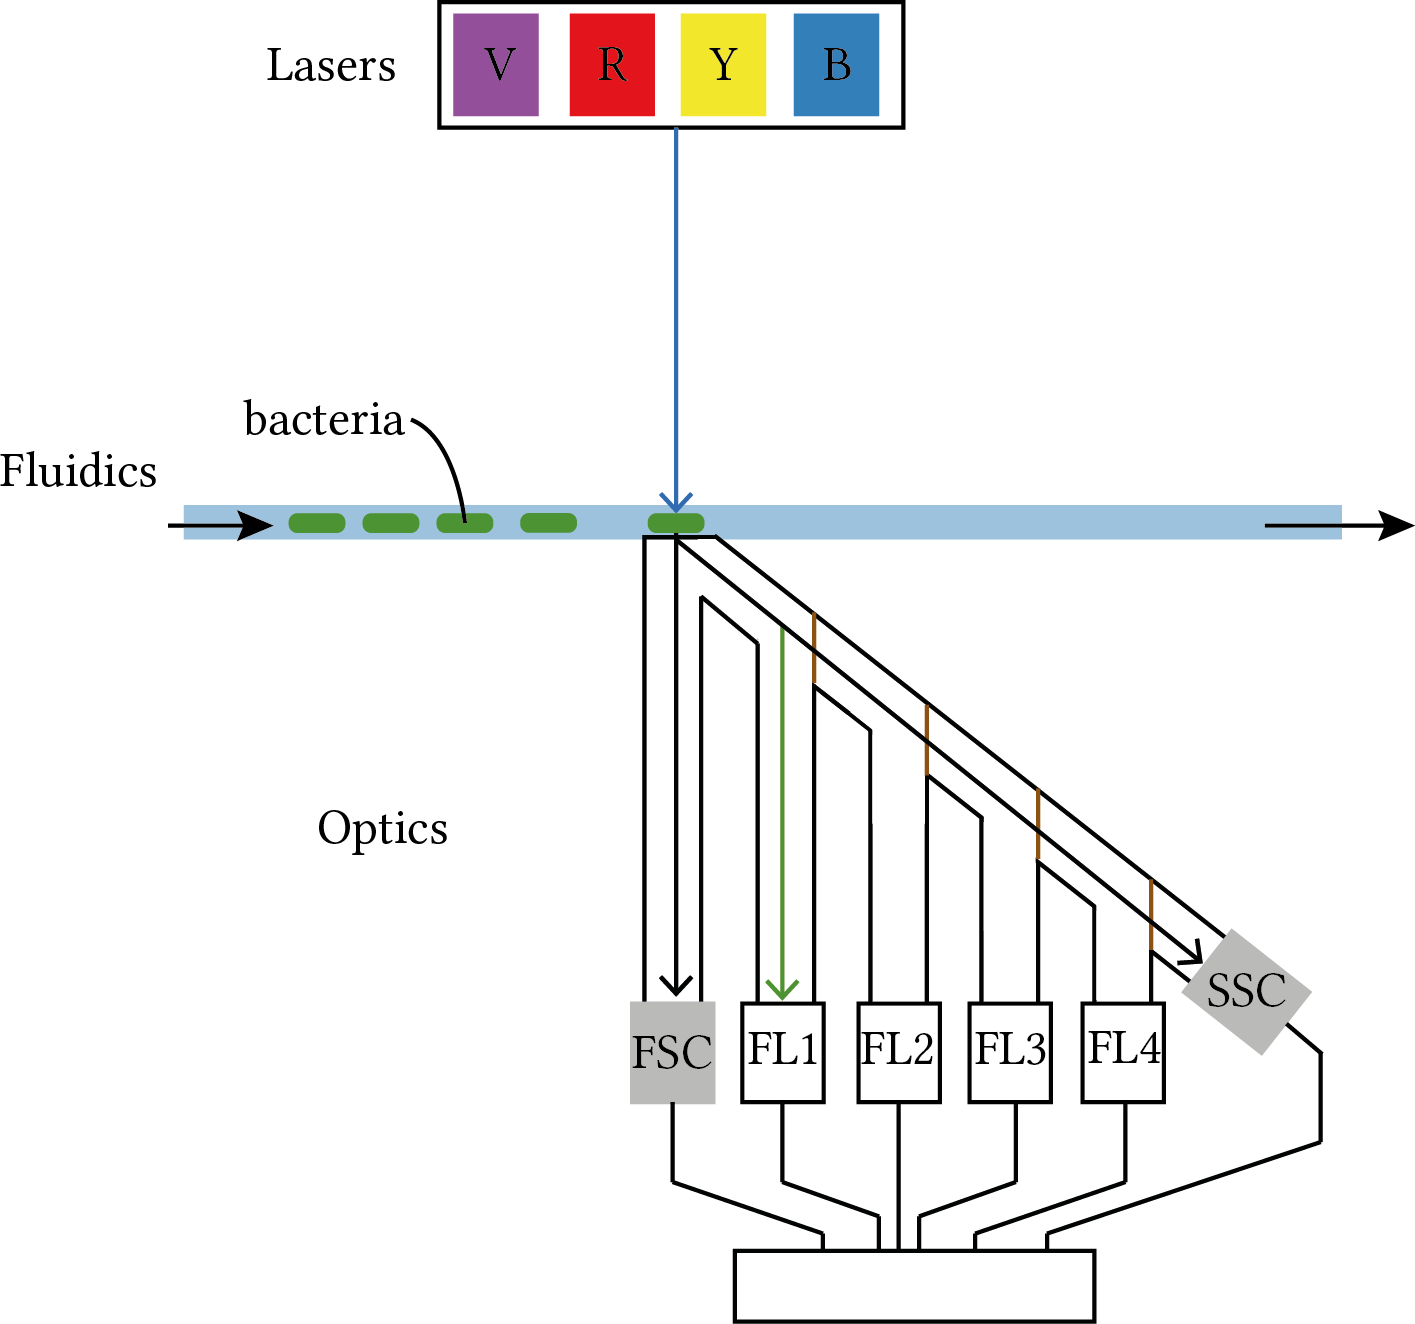
\includegraphics[scale=0.9]{../../chapters/chapterBackgr/images/flow-overview.png}
	\caption[Flow cytometry experimental setup]{\label{fig:flow_overv}Flow cytometry. A laser excites the fluorescent proteins present in each cell. The cytometer has up to 4 lasers, violet (V), red (R), yellow (Y) and blue (B). The detectors in the optics, FL1-4 pick up the signals. The cytometer also picks up size and granularity information via the forward scatter (FSC) and side scatter (SSC) detectors. Diagram adapted from~\autocite{FlowDiagram}}
	\end{center}
\end{figure*}

\section{Flow cytometry and model fitting}

Computational modelling is well known to aid the understanding  of complex systems by fitting experimental data and providing further insights and testable predictions. Experimental data is used to fit the model parameters and then the model can provide further understanding of the system and aid in the design of further experiments. Flow cytometry is used in synthetic biology for BioBrick characterisation~\autocite{Kelly:2009bj}, enzyme screening~\autocite{Choi:2014gb} and industrial  bioprocesses~\autocite{Diaz:2010kw} among others. 

Flow cytometry data presents a challenge to computational modelling as the fluorescence intensity per cell is measured rather than number of proteins. The problem with measuring fluorescence intensity is that it is a relative and not an absolute measurement. This makes the inference of parameter values challenging~\autocite{Rosenfeld:uh}. Absolute measurements would increase the predictive power of computational models~\autocite{Bower:2010jl, Cooling:2010bx}, but this type of biological data cannot be directly measured~\autocite{Kelwick:2014iy}. The fluorescence intensity values can vary between experiments due to instrument settings so they can only be used in relative terms within the same experiment. Efforts have been made to alleviate this problem by standardizing experimental methods~\autocite{Kelly:2009bj}, or using bead-based calibration to convert the arbitrary units of fluorescent proteins to MEFLs (Molecules of equivalent fluoresceine)~\autocite{Beal:2016cd}. 

%%Standardization of experimental methods in flow cytometry has aided the effort to reduce variability due to experimental setup~\autocite{Kelly:2009bj}but the successful conversion of fluorescence intensity to an absolute measurement of protein cell\textsuperscript{-1} s\textsuperscript{-1} has yet to be made successfully. 

%Another challenge that must be faced when modelling gene expression dynamics is that the stochasticity of the systems involved must be taken into account. The Gillespie algorithm~\autocite{Gillespie:1977ww} can be used to simulate a genetic system stochastically but is very computationally expensive. The unknown 


Another approach to the problem is converting the model output of GFP cell\textsuperscript{-1} s\textsuperscript{-1} to relative fluorescence intensity. This approach was first developed by~\textcite{Lillacci:2013hu}. The converted model output can then be compared to the data output from the flow cytometer. The fluorescence intensity measurements acquired via flow cytometry are treated as a sample from the distribution of the fluorescence present in the cell~\autocite{Lillacci:2013hu}. This means that the flow cytometry fluorescence distribution at each time point can be compared to the model fluorescence distribution. Here I expand the method developed by~\textcite{Lillacci:2013hu} in order to be able to apply it to flow cytometry data including two fluorescent proteins simultaneously. This new framework, ABC-Flow, can be used to fit stochastic models to flow cytometry data involving multiple species like the genetic toggle switch, but could be applied to any synthetic biology system. 


 %Using a distance metric it can be assessed whether the two samples have been drawn from the same distribution, and thus determine whether the model is a good fit to the data. This allows for the use of computational modelling on flow cytometry data. 



%ABC-Flow approaches the problem of absolute protein numbers

 
 
% ABC-Flow is a python package that uses Bayesian statistics to fit the parameters of a given model to flow cytometry time course data. The algorithm and its usage is described in Section~\ref{sec:abcflow-meth}.



%In order to characterise the~\textcite{Litcofsky:2012gr} toggle switch, I use the data collected in Section~\ref{sec:ts_time} to fit the~\textcite{Gardner:2000vha} toggle switch model, shown in Section (XXX). In order to do that, I use ABC-Flow as described in the Methods in Section~\ref{sec:abcflow-meth}.

%Prior to using ABC-Flow to fit the experimental data to a toggle switch model, ABC-Flow must be validated. In the following sections I first use randomly generated distributions to set the algorithm metrics and distances. Then I use a simulated data set to which I fit a toggle switch model and finally I use ABC-Flow to fit experimental data.  

%In the following sections I first use normal distributions to study the distance functions used in ABC-Flow. Then I use a simulated data set to which I fit a toggle switch model and finally I use ABC-Flow to fit experimental data.  


%Progress has been made in the development of computational tools for the automated analysis of flow cytometry data from the field of computational immunology~\autocite{Saeys:2016im}. These tools are used for automated gating~\autocite{Lo:2008it, Aghaeepour:2011fv, Johnsson:2016fd} as well as modelling of cellular processes over time~\autocite{Bendall:2014hs, Bagwell:2015gp}. These methods are used to track different subpopulations over time, in order to follow the underlying developmental trajectory~\autocite{Saeys:2016im} and thus cannot be applied to experiments involving uniform cell populations. 


% is necessary as flow cytometry measures the intensity of the fluorescent proteins of interest in each cell.

 %On the other hand, when simulating a model, the output is measured in number of fluorescent proteins. It is thus essential to convert the simulated signal to the same format as the data, thus convert the number of fluorescent proteins to intensity measures. 
\section{ABC-Flow algorithm development}
\label{sec:abcflow-meth}

The algorithm used in ABC-Flow is based on the same ABC algorithm as ABC-SysBio and Stability Finder described in Algorithms~\ref{alg:ABC-SMC} and~\ref{alg:StabilityFinder} respectively. ABC-Flow uses the same fundamental ABC SMC algorithm but has been adapted to be used for flow cytometry data, which required two main adaptations: Firstly, the output of the simulation module, in number of proteins, has to be converted to fluorescence intensity in order to compare it to flow cytometry data. Secondly, the distance function, measuring how close the simulated  data is from the experimental data, had to be adapted in order to compare the distance between distributions of values rather than point values. This is because flow cytometry data typically involves measurements from a large number of individual cells. The algorithm of ABC-Flow is outlined in Algorithm~\ref{alg:abc-flow} and illustrated in Figure~\ref{fig:abcflow-overv}. The modified modules of the ABC algorithm are outlined in the sections that follow.


ABC-Flow uses stochastic dynamics to simulate the model under consideration. Gene regulation is known to exhibit stochastic dynamics~\autocite{Elowitz:2002wq} due to the often low number of protein molecules involved. This can cause genetically identical cells to exhibit different phenotype and behaviour~\autocite{Weinberger:2005uv}. Therefore, ABC-Flow uses stochastic dynamics to account for this variability observed in single cell behaviour. Just as the same genetic code can produce different phenotypes in different individual cells, the same parameter values in the model will be able to produce a different behaviour due to the added intrinsic noise to the system. The assumption is made that the cells are in identical conditions and have the same genetic code, thus extrinsic noise is not taken into consideration here.  


All models are simulated stochastically using the Gillespie algorithm~\autocite{Gillespie:1977ww}. ABC-Flow simulations are implemented on \acrshort{gpu}s. The user provides an SBML model file and an input file to specify the information needed to run ABC-Flow, such as the final epsilon threshold and the priors to the parameters. The user must also provide a data file containing the flow cytometry data to which the model will be fitted. The data files used here were generated from .fcs files, which is the standard output of flow cytometers, using the R bioconductor packages flowCore~\autocite{flowCore:man}. ABC-Flow is available as a Python package, and can be downloaded from \url{https://github.com/ucl-cssb/ABC-Flow.git}. 



\begin{figure*}[htbp]
	\begin{center}
		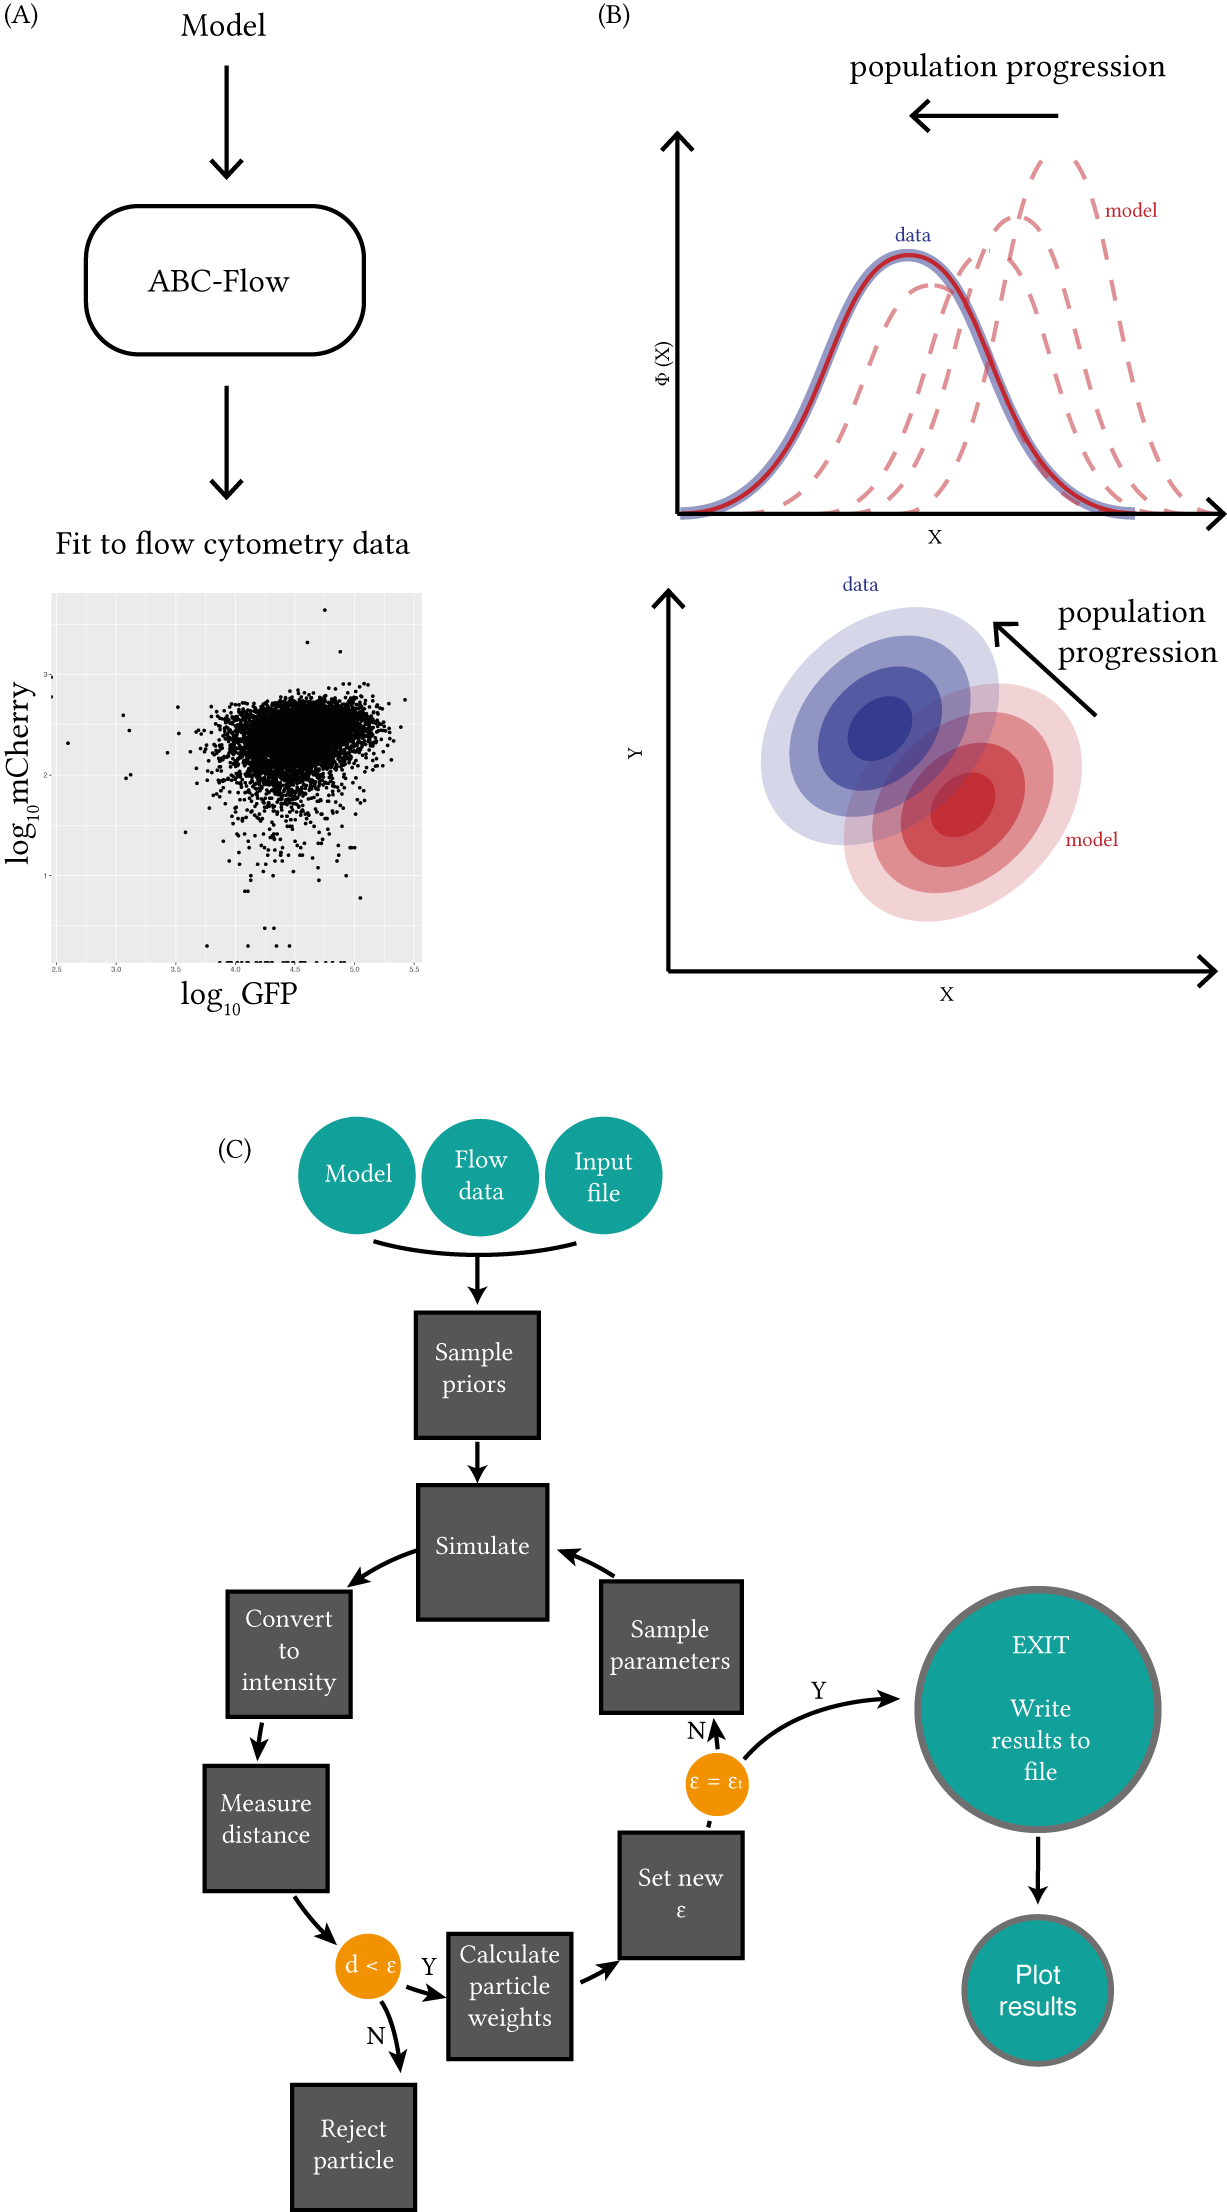
\includegraphics[scale=1.1]{../../chapters/chapterABCFlow/images/abc-flow-overv.png}
		\caption[ABC-Flow algorithm overview]{\label{fig:abcflow-overv}Overview of ABC-Flow. (A) ABC-Flow is used to fit models to experimental flow cytometry data. (B) The algorithm can be applied to 1D and 2D flow data. (C) ABC-Flow uses Approximate Bayesian Computation.}
	\end{center}
\end{figure*}





\begin{algorithm}[htbp]

\caption{ABC-Flow}
\label{alg:abc-flow}
 \begin{algorithmic}[1]
 	\Statex
% \State Read input file
%	\If{ABC-Rejection}
% 		\State Sample from priors
% 		\State Simulate model
% 		\State Convert signal to intensity
% 		\State Measure distance to data
%		\State Reject particles if d $\textgreater$ $\epsilon$.
% 		\If{number of accepted particles == number of particles}
% 			\State Exit
% 		\Else
% 			\State Return to step 3.
% 		\EndIf
% 	\EndIf
 	
 	%\If{ABC-SMC}
	\State Initialise ε
	\Let{population p}{1}
	\If{p $= 1$}
		\State Sample particles (θ) from priors
		\Else
			\State Sample particles from previous population
			\State Perturb each particle θ* using perturbation kernel $K_t$ to obtain perturbed particle θ** %, by $\pm$ half the range of the previous population (j) to obtain new perturbed population (i).

	\EndIf
	\State Simulate model using the Gillespie algorithm.
	\State Convert signal to intensity: 
	\For{each particle}
		\For{each beta}
			\For{each time point}
				\For{each fluorescent protein}
					\State Intensity $\sim$ N\bigg(signal\times$\mu$,  $\sqrt{(signal\times\sigma^2)}$\bigg)
	\EndFor				
	\EndFor	
	\EndFor	
	\EndFor	
	\State Measure distance to data
	\State Reject particles if d $\textgreater$ $\epsilon$.
    \State Calculate weight for each accepted $\theta$
	\State $w_{t}^{(i)} = \begin{cases} 1, & \mbox{if } p = 0 \\\frac{\pi(\theta_{t}^{(i)})}{\sum_{j=1}^N w_{t-1}^{(j)} K_{t}(\theta_{t-1}^{(j)}, \theta_{t}^{(i)})}, & \mbox{if } p \geq  0. \end{cases}$
	\State Normalise weights
	\State Repeat steps 3 - 15 until $ε \leq ε_T$	%EndIf
  \end{algorithmic}
\end{algorithm}
\clearpage
\subsection{Intensity Calculation}

The units of the result of the stochastic simulations is in number of molecules. On the other hand, flow cytometry data units are in the form of fluorescence intensity. For ABC-Flow, the simulation results are converted to intensity in order to be able to compare the data to the simulations. In order to do this two additional parameters are defined, intensity μ and intensity σ, for each fluorescent protein used. To convert the number of fluorescent proteins to intensity, random samples are drawn from a normal distribution

\begin{align}
	X\sim N\Big(n_{FP}\mu, \sqrt{(n_{FP}\sigma^2)}\Big), \label{eq:intens}
\end{align}
where $n_{FP}$ is the number of fluorescent proteins. These parameters are estimated from the data along with the model parameters. An illustration of the intensity calculation is shown in Figure~\ref{fig:intensity_calc}. The intensity conversion also includes the addition of background signal. This represents the intensity signal detected by flow cytometers when no fluorescent proteins are present~\autocite{Lillacci:2013hu}. The level of background fluorescence is determined by using controls during the flow cytometry experiment, and is added to the intensity signal of each fluorescent protein in the model.

\begin{figure*}[tb]
	\begin{center}
		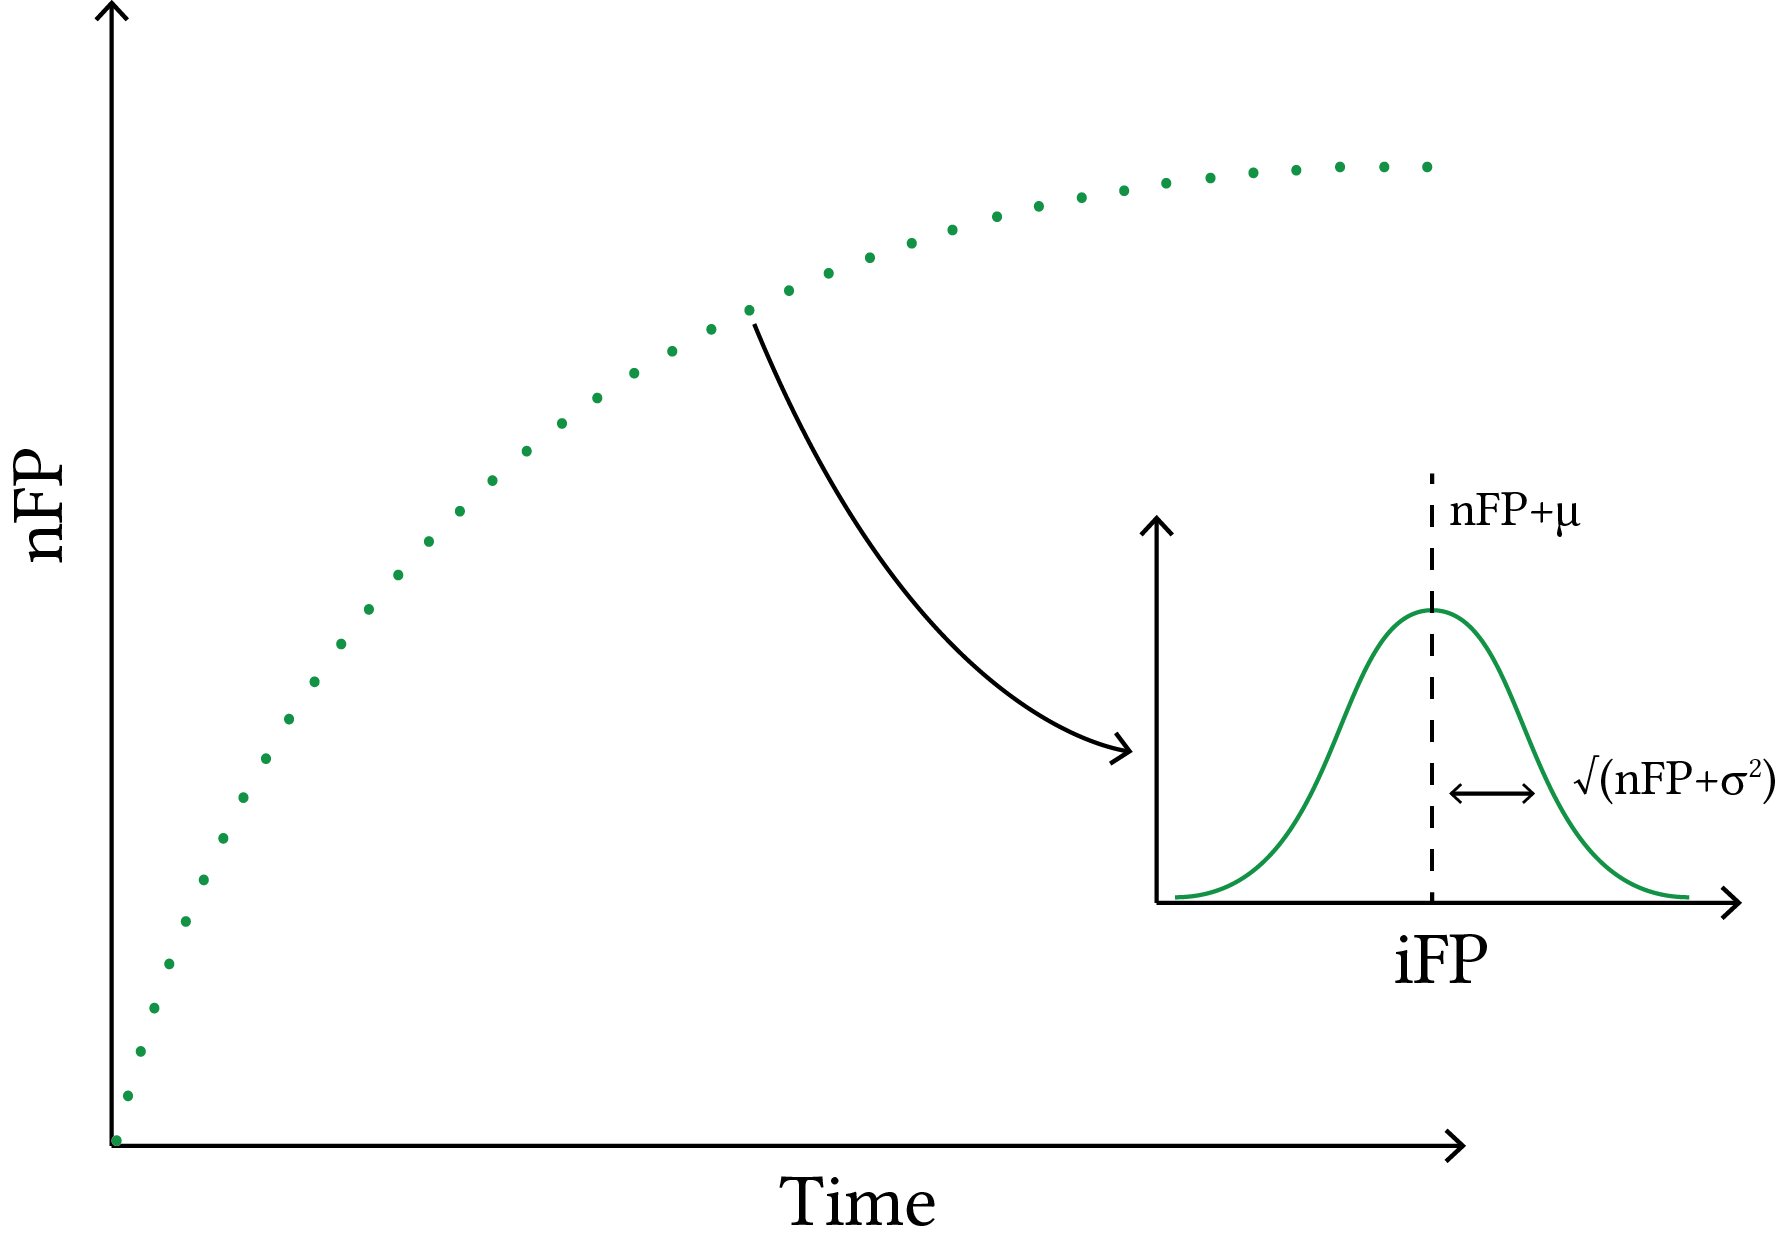
\includegraphics[scale=0.5]{../../chapters/chapterABCFlow/images/intensity_calc.png}
		\caption[Converting the number of fluorescent proteins to intensity]{\label{fig:intensity_calc}Converting the number of fluorescent proteins (n\textsubscript{FP}) to the intensity (i\textsubscript{FP}) is done by drawing from a normal distribution, as shown in Equation~\ref{eq:intens}.}
	\end{center}
\end{figure*}
\clearpage
\subsection{Distance Calculation}

In order to compare the flow cytometry data to the model generated data, I developed a distance measure. This distance measure should be able to determine whether two datasets are sufficiently close to each other to be able to be assume that they have been drawn from the same distribution. The measure should also give an estimate of how different the two data sets are, and thus get larger as two data sets are drawn from increasingly different distributions. %Finally the distance measure should be applicable to one and two dimensional distributions, and be comparable between the two. 


In order to select an appropriate distance metric, I tested three methods using simulated distributions. First, the calculation of the kernel distance between the simulated and experimental data was considered. As can be seen in the results shown in Section~\ref{sec:dist_kernel} the distance value did not monotonically decrease with increasingly similar distributions therefore it was not considered a good method for this application. I then implemented the \acrfull{ks} distance, as used in~\textcite{Lillacci:2013hu}. The \acrshort{ks} test is a non-parametric statistic test that determines whether two data sets were drawn from the same underlying distributions by computing the largest distance between the empirical distribution functions of the two datasets. This was shown to work well when  comparing simulated data to flow cytometry data~\autocite{Lillacci:2013hu}. Nevertheless, the \acrshort{ks} test does not scale well for multidimensional distributions. This is because there is no unique way to order the data points to calculate the largest distance. As is discussed in Section~\ref{sec:dist_ks}, the \acrshort{ks} test did not perform well on two-dimensional distributions. Finally, I tested the Wald-Wolfowitz test for two-dimensional distributions. This was found to work well during the theoretical tests. Therefore, I implemented the Kolmogorov-Smirnov distance for one-dimensional datasets and the Wald-Wolfowitz for two-dimensional datasets in ABC-Flow. Each distance metric is described in more detail in the following sections.  

\label{sec:dist}
\subsubsection{Kernel distance}
\label{sec:dist_kernel}
In order to measure the distance between the flow cytometry data and the fitted model, Algorithm~\ref{alg:dist} was developed. The algorithm consists of defining a grid from the minimum to the maximum value of the data. A gaussian kernel was then fit to the flow and simulated data. The distance between the two kernels is given by:

\begin{align*}%
	d = \sum_{i=xmin}^{xmax} (fD_i - fS_i)^2,
\end{align*}
where $fD_i$ is the kernel of the flow data at each value of x and $fS_i$ the kernel of the simulaed data. An illustration of the distance calculation is shown in Figure~\ref{fig:old_dist}.



\begin{figure}[tb]
\centering
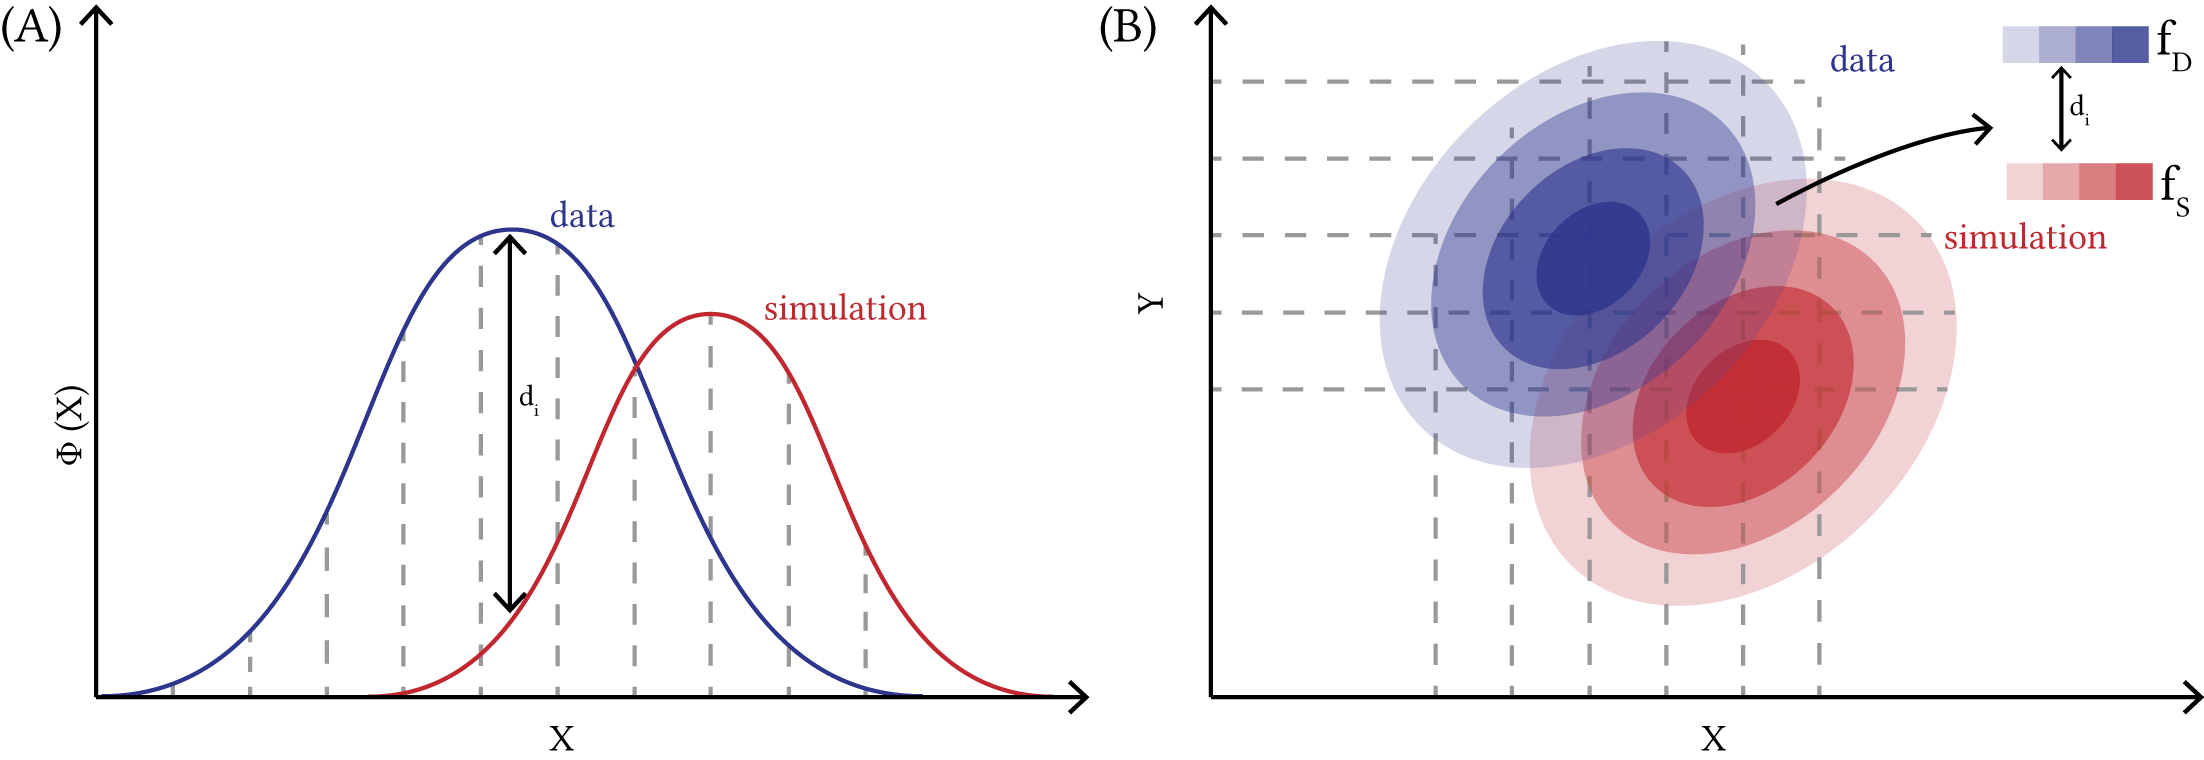
\includegraphics[scale=0.8]{../../chapters/chapterABCFlow/images/old_distance.png}
\caption[Kernel distance]{\label{fig:old_dist}Calculating the distance between two distributions using the kernel distance in (A) 1D and (B) 2D. }
\end{figure}



\begin{algorithm}[tb]
\caption{Kernel distance calculation}
\label{alg:dist}
 \begin{algorithmic}[1]
    \Statex
	\Let {xx}{min(data):max(data):ngrid} 
	\State kD = kernel density estimation(data)
	\State kS = kernel density estimation(simulations)
	\State fD = kD(xx)
	\State fS = kS(xx)    
	\State $d = \sum(fD-fS)^2$
  \end{algorithmic}
\end{algorithm}

In order to test this distance metric samples were drawn from two uniform distributions with varying mean and standard deviation. Algorithm~\ref{alg:dist} was then used to calculate the distance between the different distributions. First, Algorithm~\ref{alg:dist} was tested by drawing samples from two distributions with an increasingly different mean. This is done to determine the dynamical range of the distance calculation.

\begin{figure}[htb]
\centering
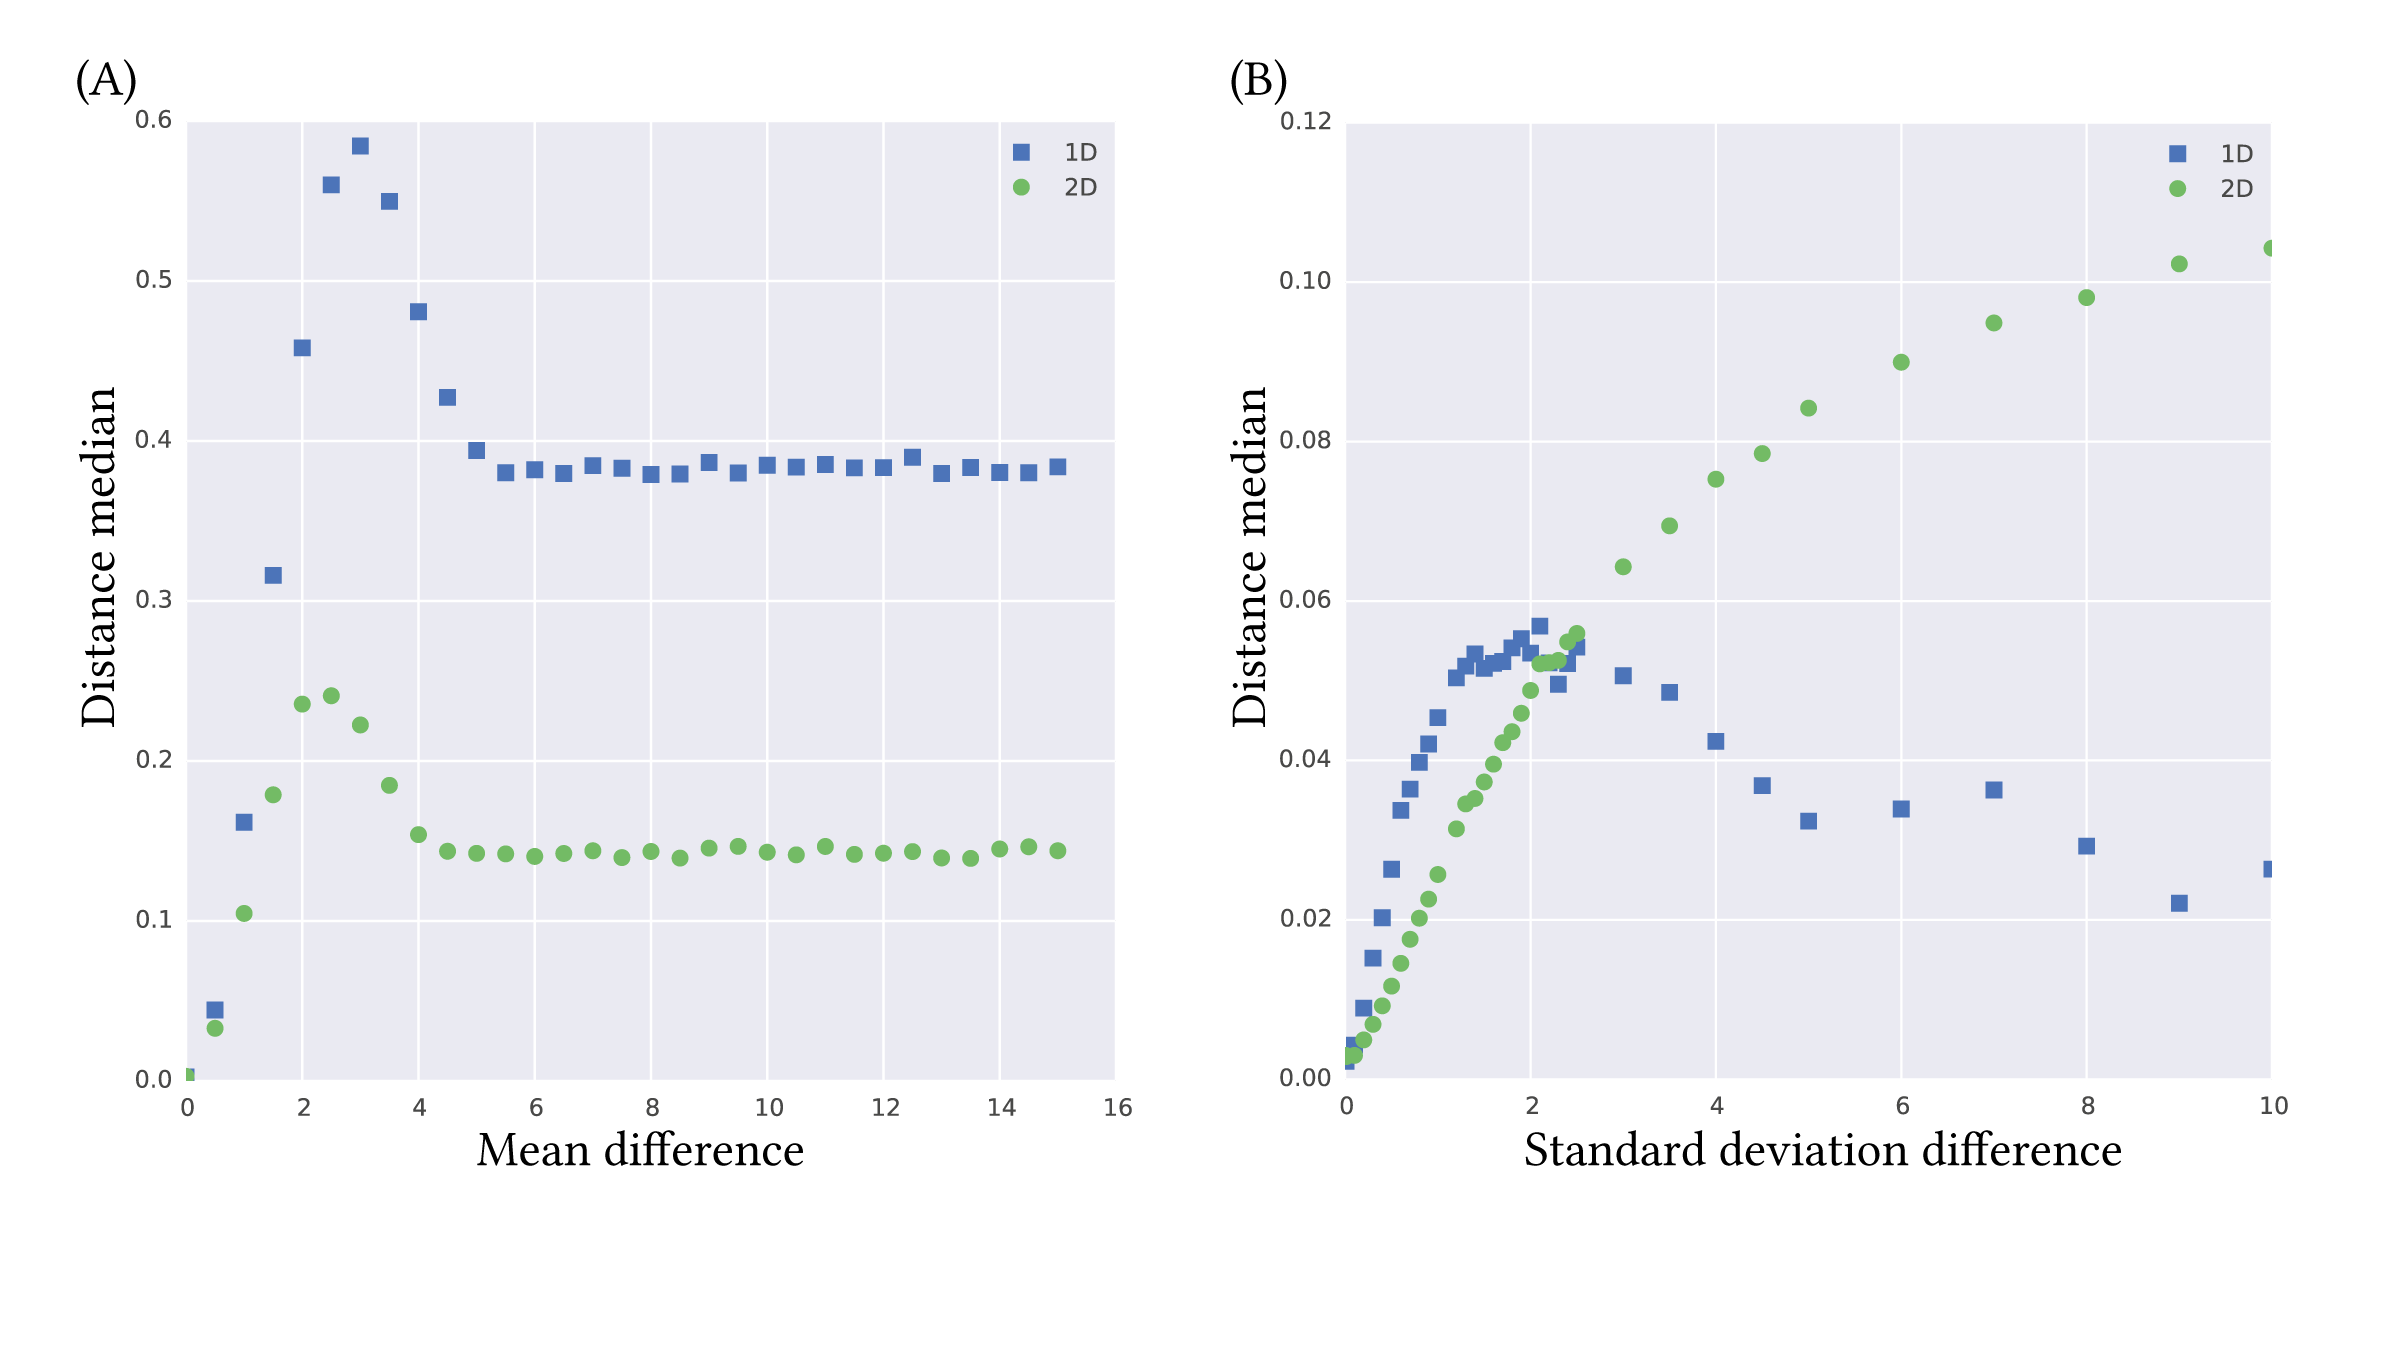
\includegraphics[scale=0.7]{../../chapters/chapterABCFlow/images/mus_sigmas-01.png}
\caption[Range of distance values using the kernel distance]{\label{fig:epsilon_mu_s_diff}(A) The range by which distance varies as the difference between the means of the distributions increases. (B) The median of the distance distributions varies by a small amount with increasing difference in the standard deviation of the distributions.}
\end{figure}

From Figure~\ref{fig:epsilon_mu_s_diff} we see that the distance value decreases with increasing mean difference of the two distributions. As the difference between the means increases, the distance value reaches a peak when the difference is at 3. From that point, as the mean difference increases, distance values decrease until they reach a plateau at epsilon = 0.38 in the 1D case and epsilon = 0.14 in the 2D case. Next I tested the distance calculation by comparing bimodal distributions. Two bimodal distributions are generated with increasingly different mean, in 1D and 2D. 


\begin{figure}[tb]
\centering
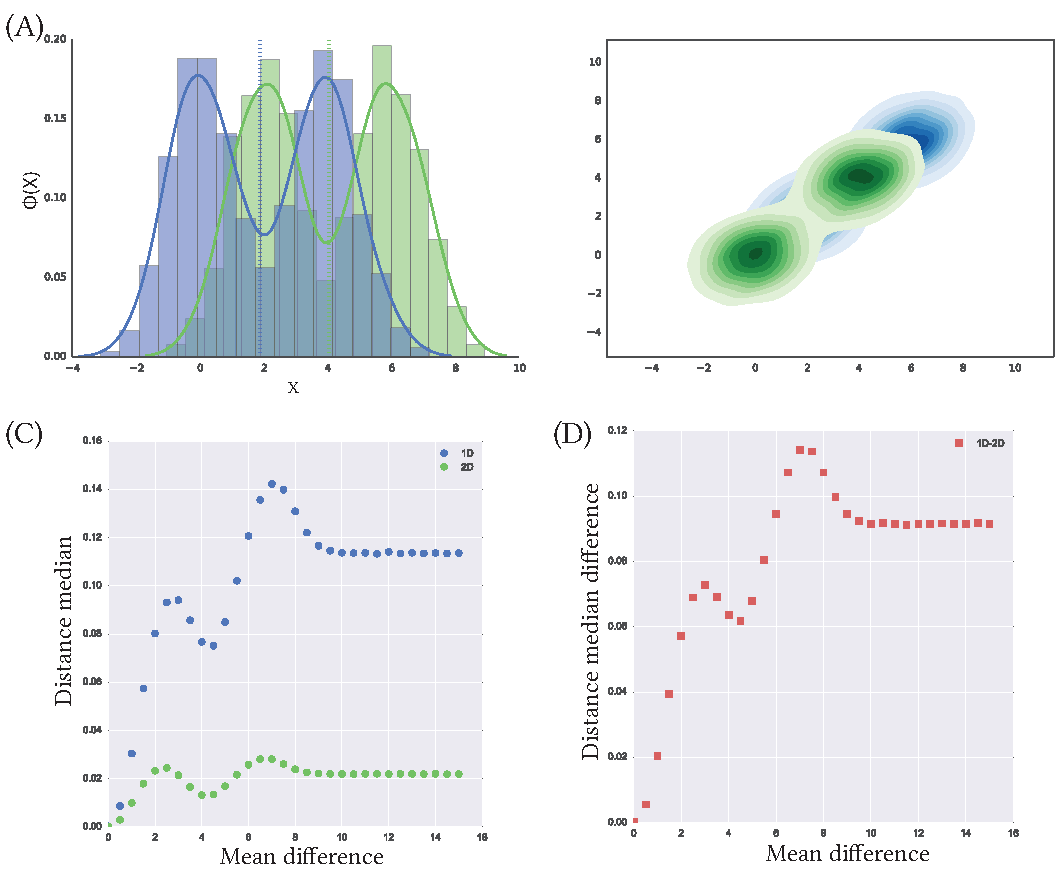
\includegraphics[scale=0.7]{../../chapters/chapterABCFlow/images/multimodal_musd.pdf}
\caption[Distance value ranges of bimodal distributions using the kernel distance]{\label{fig:multimodal_musd}Comparing the 1D and 2D distances between bimodal distributions. (A) and (B) show samples of the bimodal distributions compared in 1D and 2D respectively with a mean difference of 4 between simulations and data. (C) The range by which the distance median varies as the difference between the mean of the distributions increases. (D) The difference between the distances calculated in 1D and 2D is not constant.}

\end{figure}

Similar to the normal distribution, for the bimodal distributions shown in Figure~\ref{fig:multimodal_musd} we find that the distance values do not increase linearly. There are two peaks in the distances distribution, one at mean difference = 3 and one at mean difference = 6. The distance values then decline until they reach a plateau. The distance values do not have a large range of values, for either the 1D or 2D cases. We also find that the difference in the distance values between the 1D and 2D cases is not constant. Finally, I studied how these distance functions perform when comparing a bimodal with a normal distribution. A bimodal distribution is generated and a series of normal distributions with increasing mean, in 1D and 2D. From Figure~\ref{fig:multimodal_v_normal} we find that the distance calculation is the lowest when the mean of the normal distribution corresponds to the μ of one of the two peaks in the bimodal distribution and the highest when there is no overlap between the distributions.


\begin{figure}[tb]
\centering
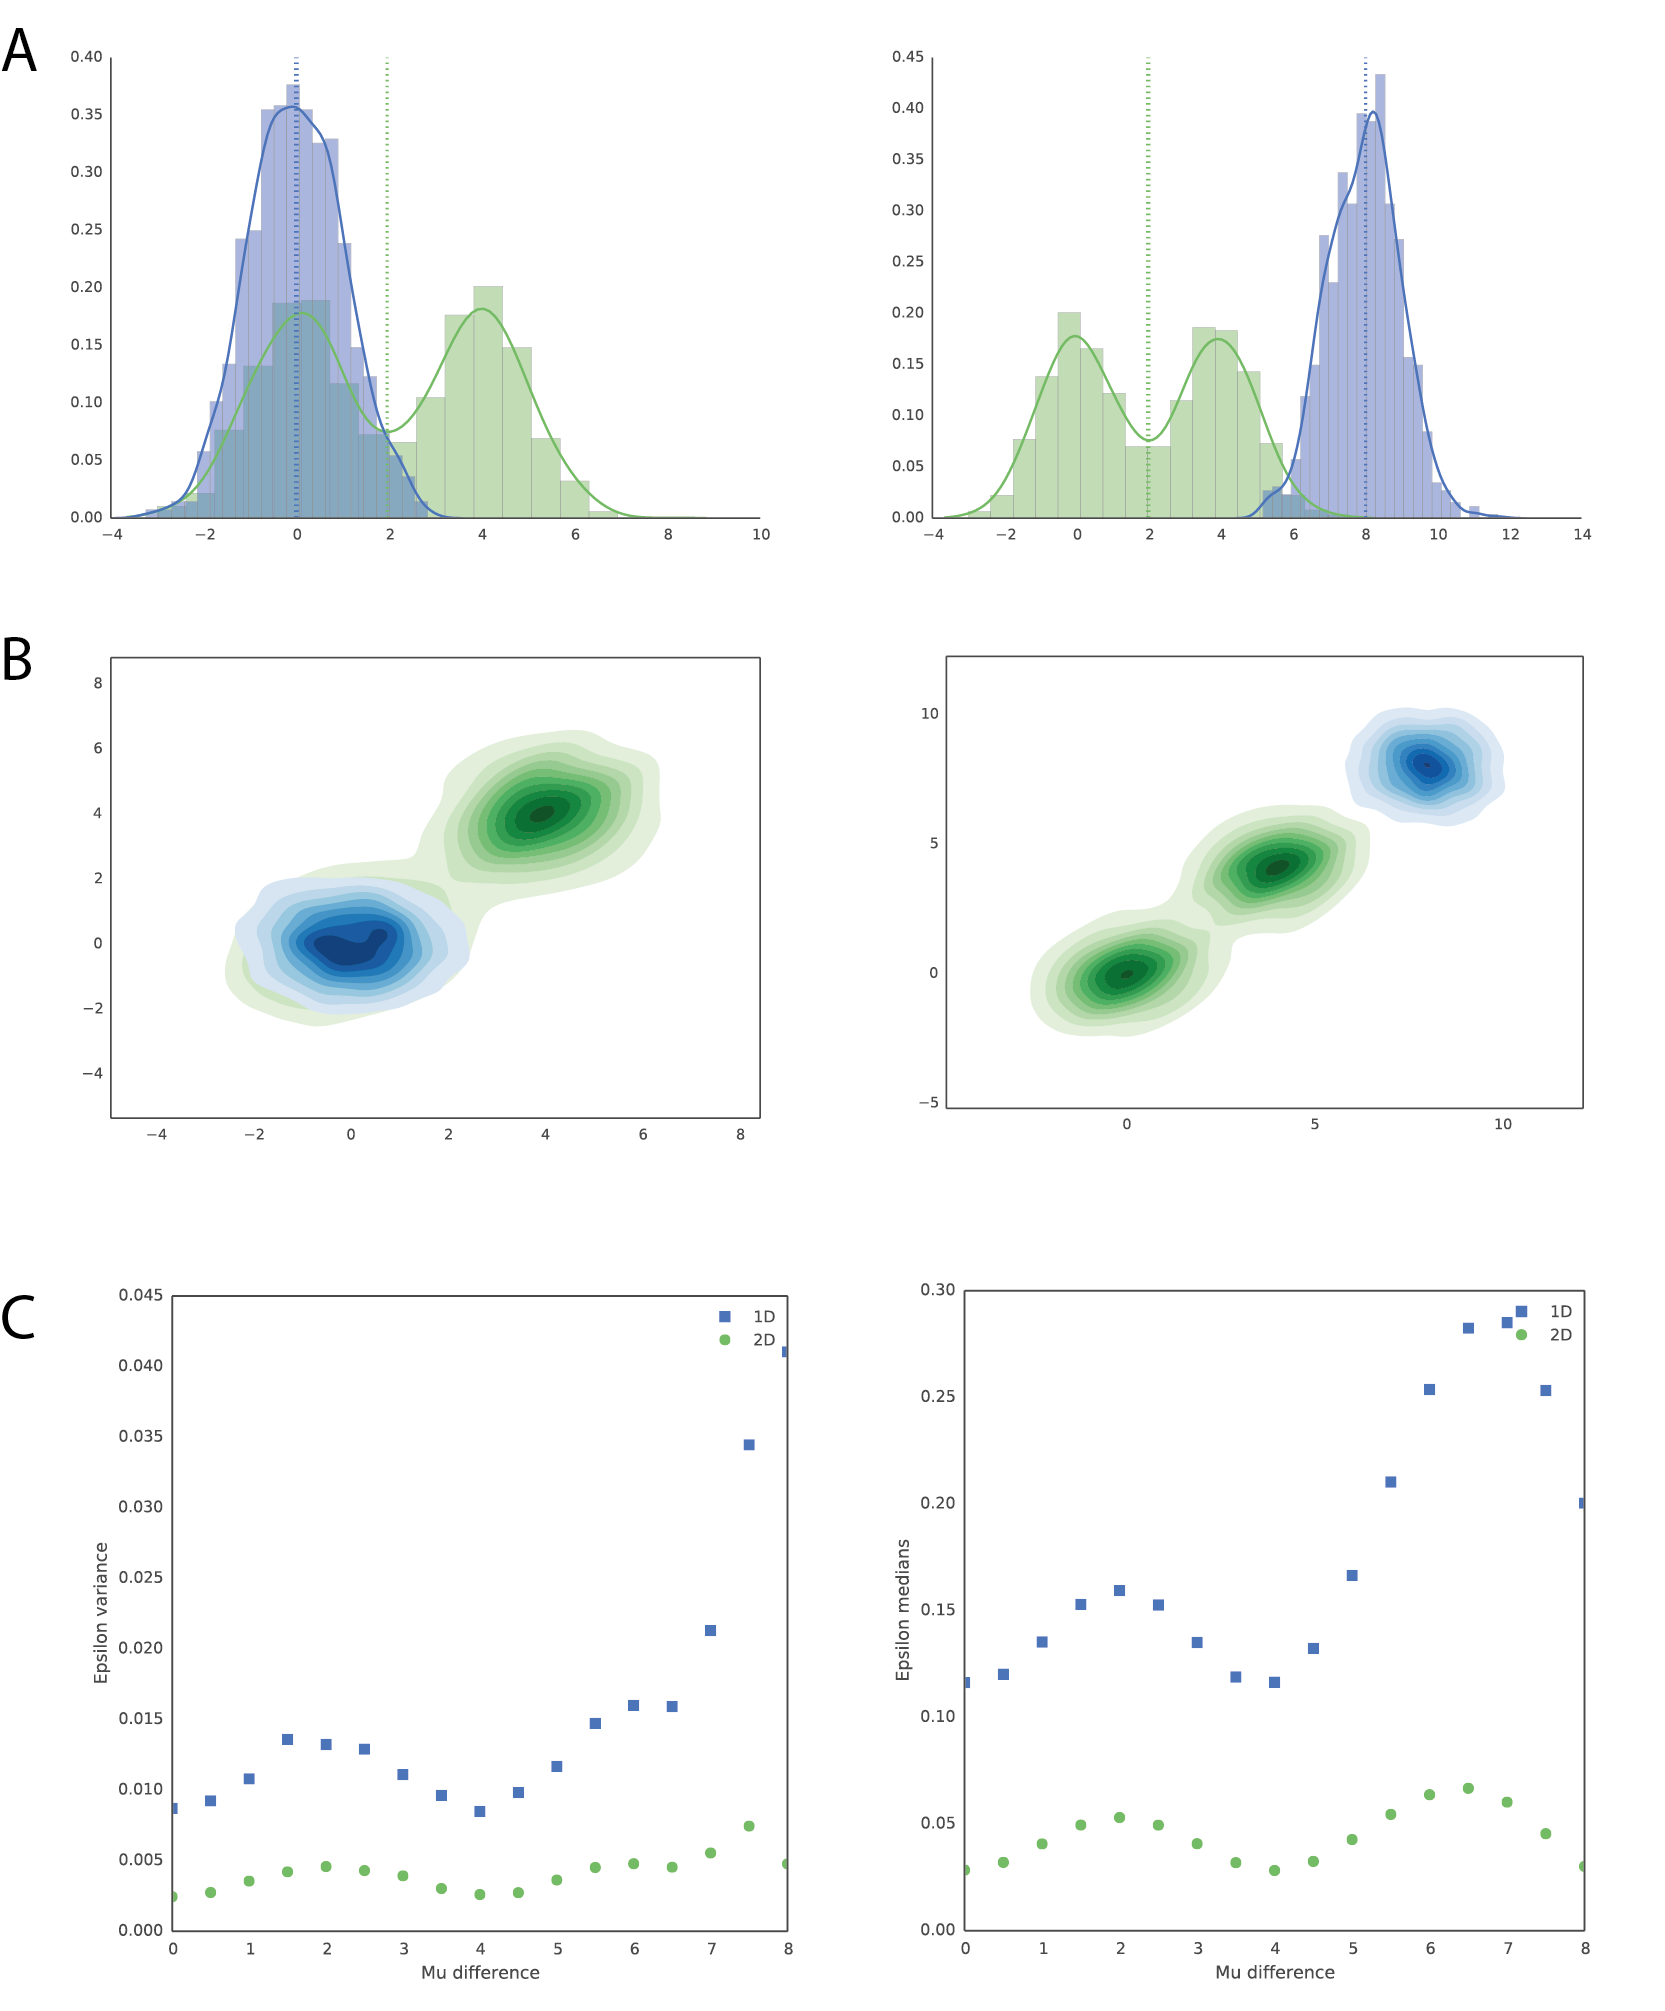
\includegraphics[scale=0.7]{../../chapters/chapterABCFlow/images/multimodal_v_normal.png}
\caption[Distance value ranges of bimodal and uniform distributions using the kernel distance]{Comparing a multimodal to a normal distribution, in 1D and 2D. (A, B) The mean of the normal distribution is varied from equal to the mean of the first peak of the bimodal distribution to beyond the range of the bimodal distribution. (C) Distance median and variance are at the lowest when the mean of the normal distribution is equal to the mean of one of the peaks of the bimodal distribution. }
\label{fig:multimodal_v_normal}
\end{figure}



From Figures~\ref{fig:epsilon_mu_s_diff}-\ref{fig:multimodal_v_normal} I conclude that Algorithm~\ref{alg:dist} is not a good measure for distance to be used in ABC-Flow. If Algorithm~\ref{alg:dist} was used in order to minimize the distance between two distributions that start off with very different means, the distance between the two distributions will not be sufficiently minimized. This stems from the fact that ABC-Flow works by iteratively making the epsilon threshold smaller. As can be seen in Figure~\ref{fig:epsilon_mu_s_diff}, if the two distributions have a large difference in the means, (>6) it would not be possible to overcome the peak that is created when the mean difference is at 3. Distance values increase before the decrease again, which will be a problem in ABC-Flow. Therefore a different distance calculation was developed.   
%%%%%%%%%%
\subsubsection{Kolmogorov-Smirnov distance}
\label{sec:dist_ks}

In order to avoid the problems that arose from the distance calculation described in Section~\ref{sec:dist_kernel} I implemented a different distance calculation for ABC-Flow. I used a Python implementation of the Kolmogorov-Smirnov two sample test for the 1D case~\autocite{Kolmogorov:1933}. The \acrshort{ks} distance between two distributions is equal to the largest distance between the empirical distribution functions of the two samples, as shown in Equation~\ref{eq:ks1d}.%illustrated in Figure~\ref{fig:ks-dist} and Equation~\ref{eq:ks1d}.

\begin{align}
\label{eq:ks1d}
D_{n,n'}=\sup _{x}|F_{1,n}(x)-F_{2,n'}(x)|.
\end{align}

\noindent For the 2D case the distance was calculated by using the 2D Kolmogorov-Smirnov two sample test. The algorithm was developed by~\textcite{Fasano:1987hg} and the Python implementation developed by~\textcite{Syrtis2016}. 

\begin{figure*}[tb]
\begin{center}
	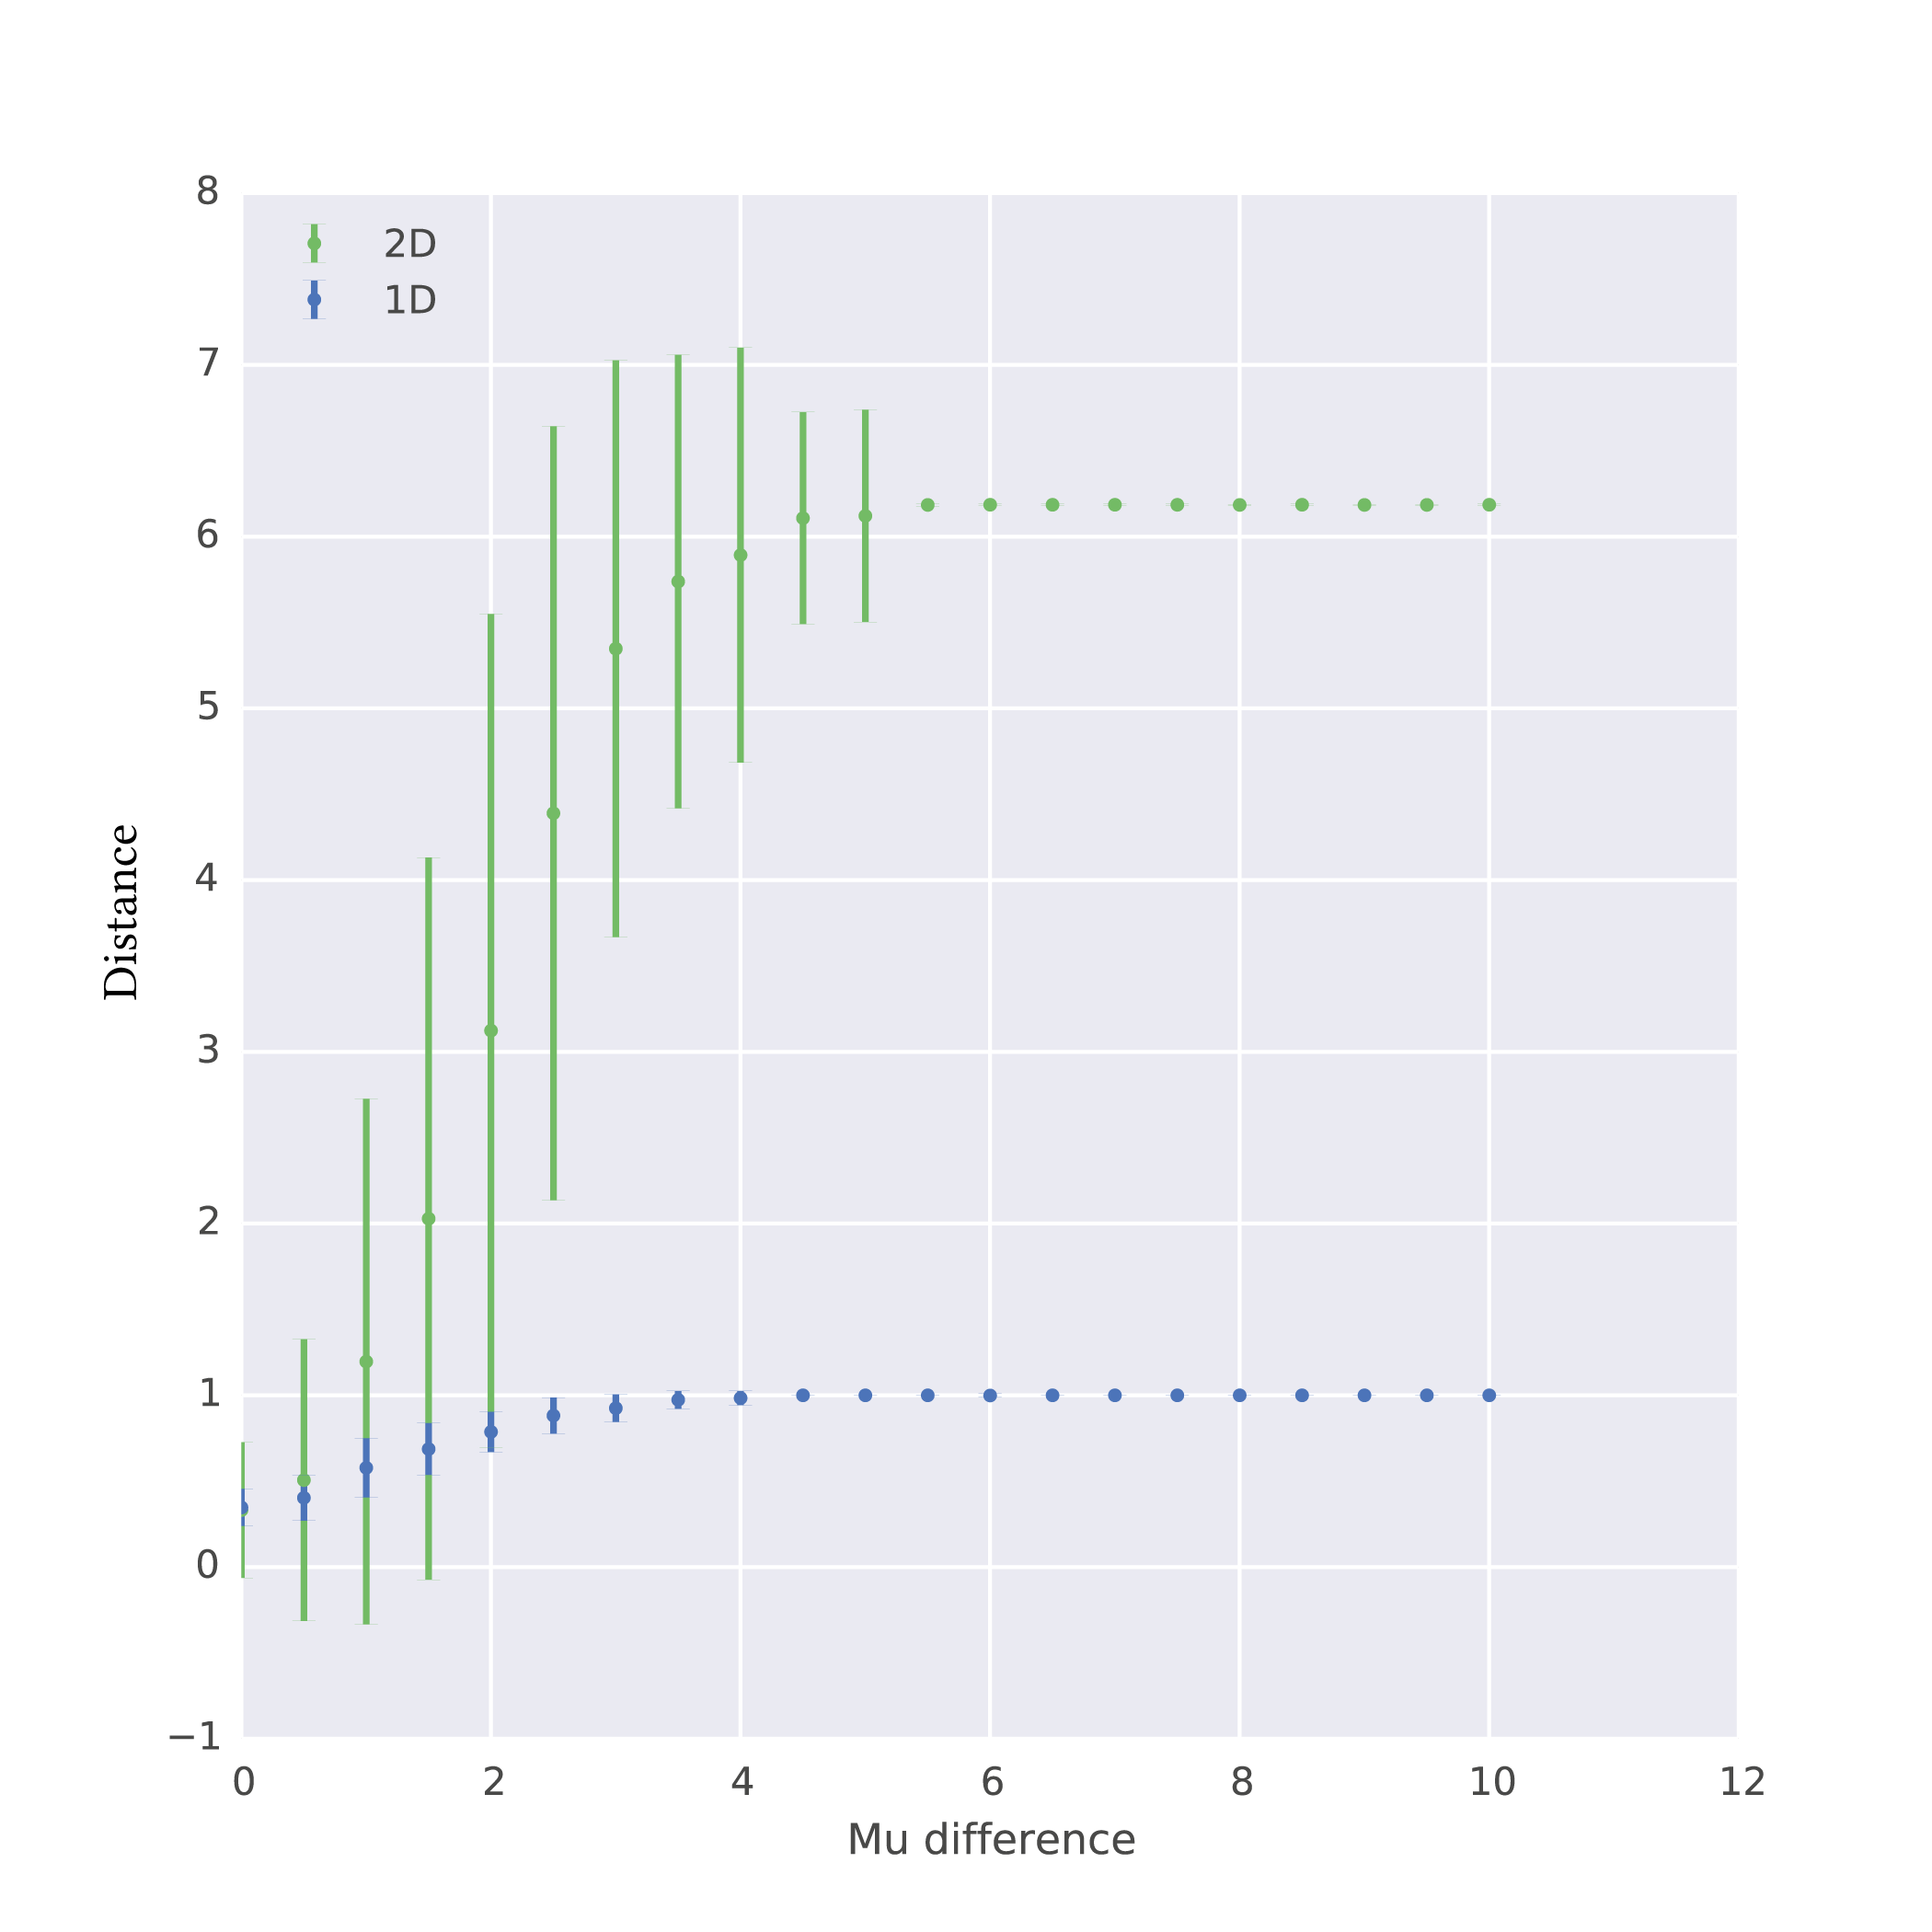
\includegraphics[scale=0.5]{../../chapters/chapterABCFlow/images/epsilon_uniform_musd_KS2sam.png}			
	\caption[Range of distance values using the Kolmogorov-Smirnov distance]{\label{fig:ks-1d2d}The Kolmogorov-Smirnov distance function was tested in 1D (blue) and 2D (green). Two data sets were generated with increasing mean difference, and the Kolmogorov-Smirnov two-sample test was applied to compute the distance between the two.}
	\end{center}
\end{figure*}

This distance calculation was tested to determine whether it is an appropriate distance function to use in ABC-Flow. Two datasets were drawn from normal distributions with increasingly different means. The \acrshort{ks} test was then used to calculate the distance between the data sets. This was carried out in 1D and 2D. The results are shown in Figure~\ref{fig:ks-1d2d}. The distances of the 1D Kolmogorov-Smirnov calculation increased with increasing mean difference until it reached a plateau when the two distributions were very different. This distance function is therefore preferable over the kernel distance tested above. As the epsilon threshold is lowered at each iteration the difference between the two data sets decreases. Therefore the 1D KS statistic was used in ABC-Flow. 

This test did not scale well in two dimensions. The variability in the calculation of the distance between data sets originating from distributions with known distance is large relative to the range of values the calculation can take. The \acrshort{ks} is problematic in higher dimensions as there are  $2^d − 1$ ways of ordering the data points and defining a cumulative distribution function, where $d$ is the number of dimensions~\autocite{Lopes:2007vk}. To alleviate the above shortcomings of the multi-dimensional generalisation of the Kolmogorov-Smirnov test, a different distance calculation was used for the 2D case. The Kolmogorov-Smirnov test for the 1D case was used in ABC-Flow as it performed well in the testing shown here. 

 %This was further confirmed when testing this distance on simulated data, where no parameter identifiability was observed (data shown in Appendix~\ref{ap:figures}).
 
\subsubsection{Wald-Wolfowitz distance}

For the 2D case the distance was calculated by using the multivariate Wald-Wolfowitz test~\autocite{Friedman:1979vm}. This is a generalisation of the Wald-Wolfowitz test proposed by~\autocite{Wald:1940wt}, a non-parametric test to determine whether two data sets were drawn from the same distribution. This test works by computing the minimum spanning tree of the pooled samples. Any edge whose nodes originated from different samples are removed, and the number of \textit{runs} (R) is then defined by the number of disjointed subtrees~\autocite{Friedman:1979vm}. If the number of \textit{runs} is small, then the null hypothesis that the two samples originated from the same distribution cannot be rejected. The quantity W for two samples of length m and n is given by 
 
\begin{align}
W = \frac{R - 2\frac{mn}{N}-1}{\sqrt{\frac{2mn(2mn-N)}{N^2(N-1)}}},
\end{align}
where $N = m + n$ and $R$ is the number of \textit{runs}. A Python implementation of the multivariate Wald-Wolfowitz test by~\textcite{Monaco:2014wx} was used here. This is a variation of the Wald-Wolfowitz test that can be efficiently applied to larger data sets. 

%\begin{figure*}[htbp]
%	\begin{center}
%		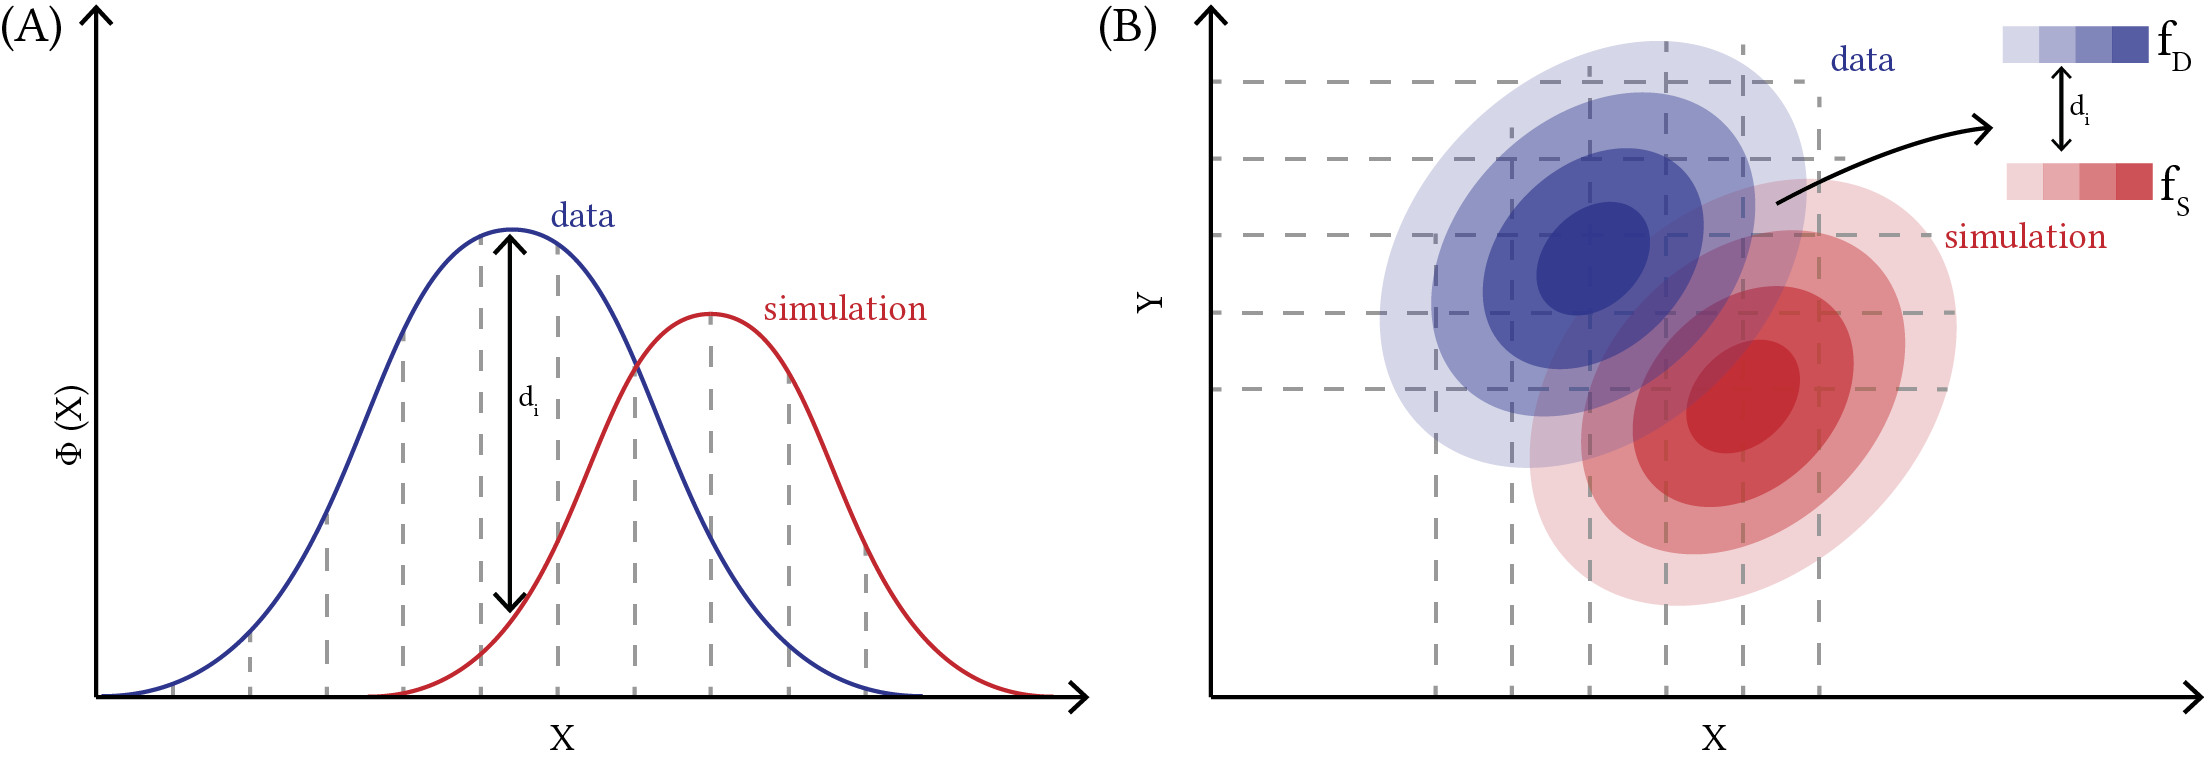
\includegraphics[scale=0.8]{../../chapters/chapterABCFlow/images/KS-dist.png}
%		\caption[LoF caption]{\label{fig:ks-dist}:The Kolmogorov-Smirnov distance function used to calculate the distance between distributions in the 1D (A) and 2D (B) cases.}
%	\end{center}
%\end{figure*}
%\clearpage

%Here I simulate two normal distributions, with identical mu and sigma, and calculate the distance between the two using the distance measure used in ABC-Flow. Doing this 1000 times, we then plot the distribution of epsilon. By doing that we can calculate the variance of the epsilon distribution, and find out the error that can be expected when measuring the distance in ABC-Flow. By doing that in 1D and in 2D we can compare the epsilon variances. 
I tested this distance calculation in a similar way as Section~\ref{sec:dist_kernel}. First, the two data sets are drawn from increasingly different distributions, and the distance between them calculated. As shown in Figure~\ref{fig:epsilon_mud}D, the distance is 0 when the two datasets are drawn from the same distribution. The distance calculation reached a plateau at distance = 140 when the mean difference was 4 or larger. The 1D distance is also shown in Figure~\ref{fig:epsilon_mud}C in order to compare the two calculations, but the 1D distance was computed using the Kolmogorov-Smirnov distance described in Section~\ref{sec:dist_ks}.

To further study the distance calculation used in ABC-Flow, two normal distributions were simulated, with $\mu=0$ and $\sigma=1$ and distance between them calculated using the Kolmogorov-Smirnov test in the 1D case and the Wald-Wolfowitz test in the 2D case. Doing this multiple times, the expected variation in distance values for identical distributions can be calculated. This represents the variation that can be expected when measuring distance in ABC-Flow. As can be seen in Figure~\ref{fig:epsilon_boxplt}, the range of distance values obtained in the 1D case is small. For the 2D case, the distance values obtained vary more than in the 1D case, but it is still small relative to the range of values that the Wald-Wolfowitz test can take shown in Figure~\ref{fig:epsilon_mud}. 
%As shown in Figure~\ref{fig:epsilon_mud}D, as the number of samples drawn from each distribution increases, the standard deviation of the distance calculations decreases in the 1D case. This trend is less obvious in the 2D case.

 
\begin{figure}[tb]
\centerfloat
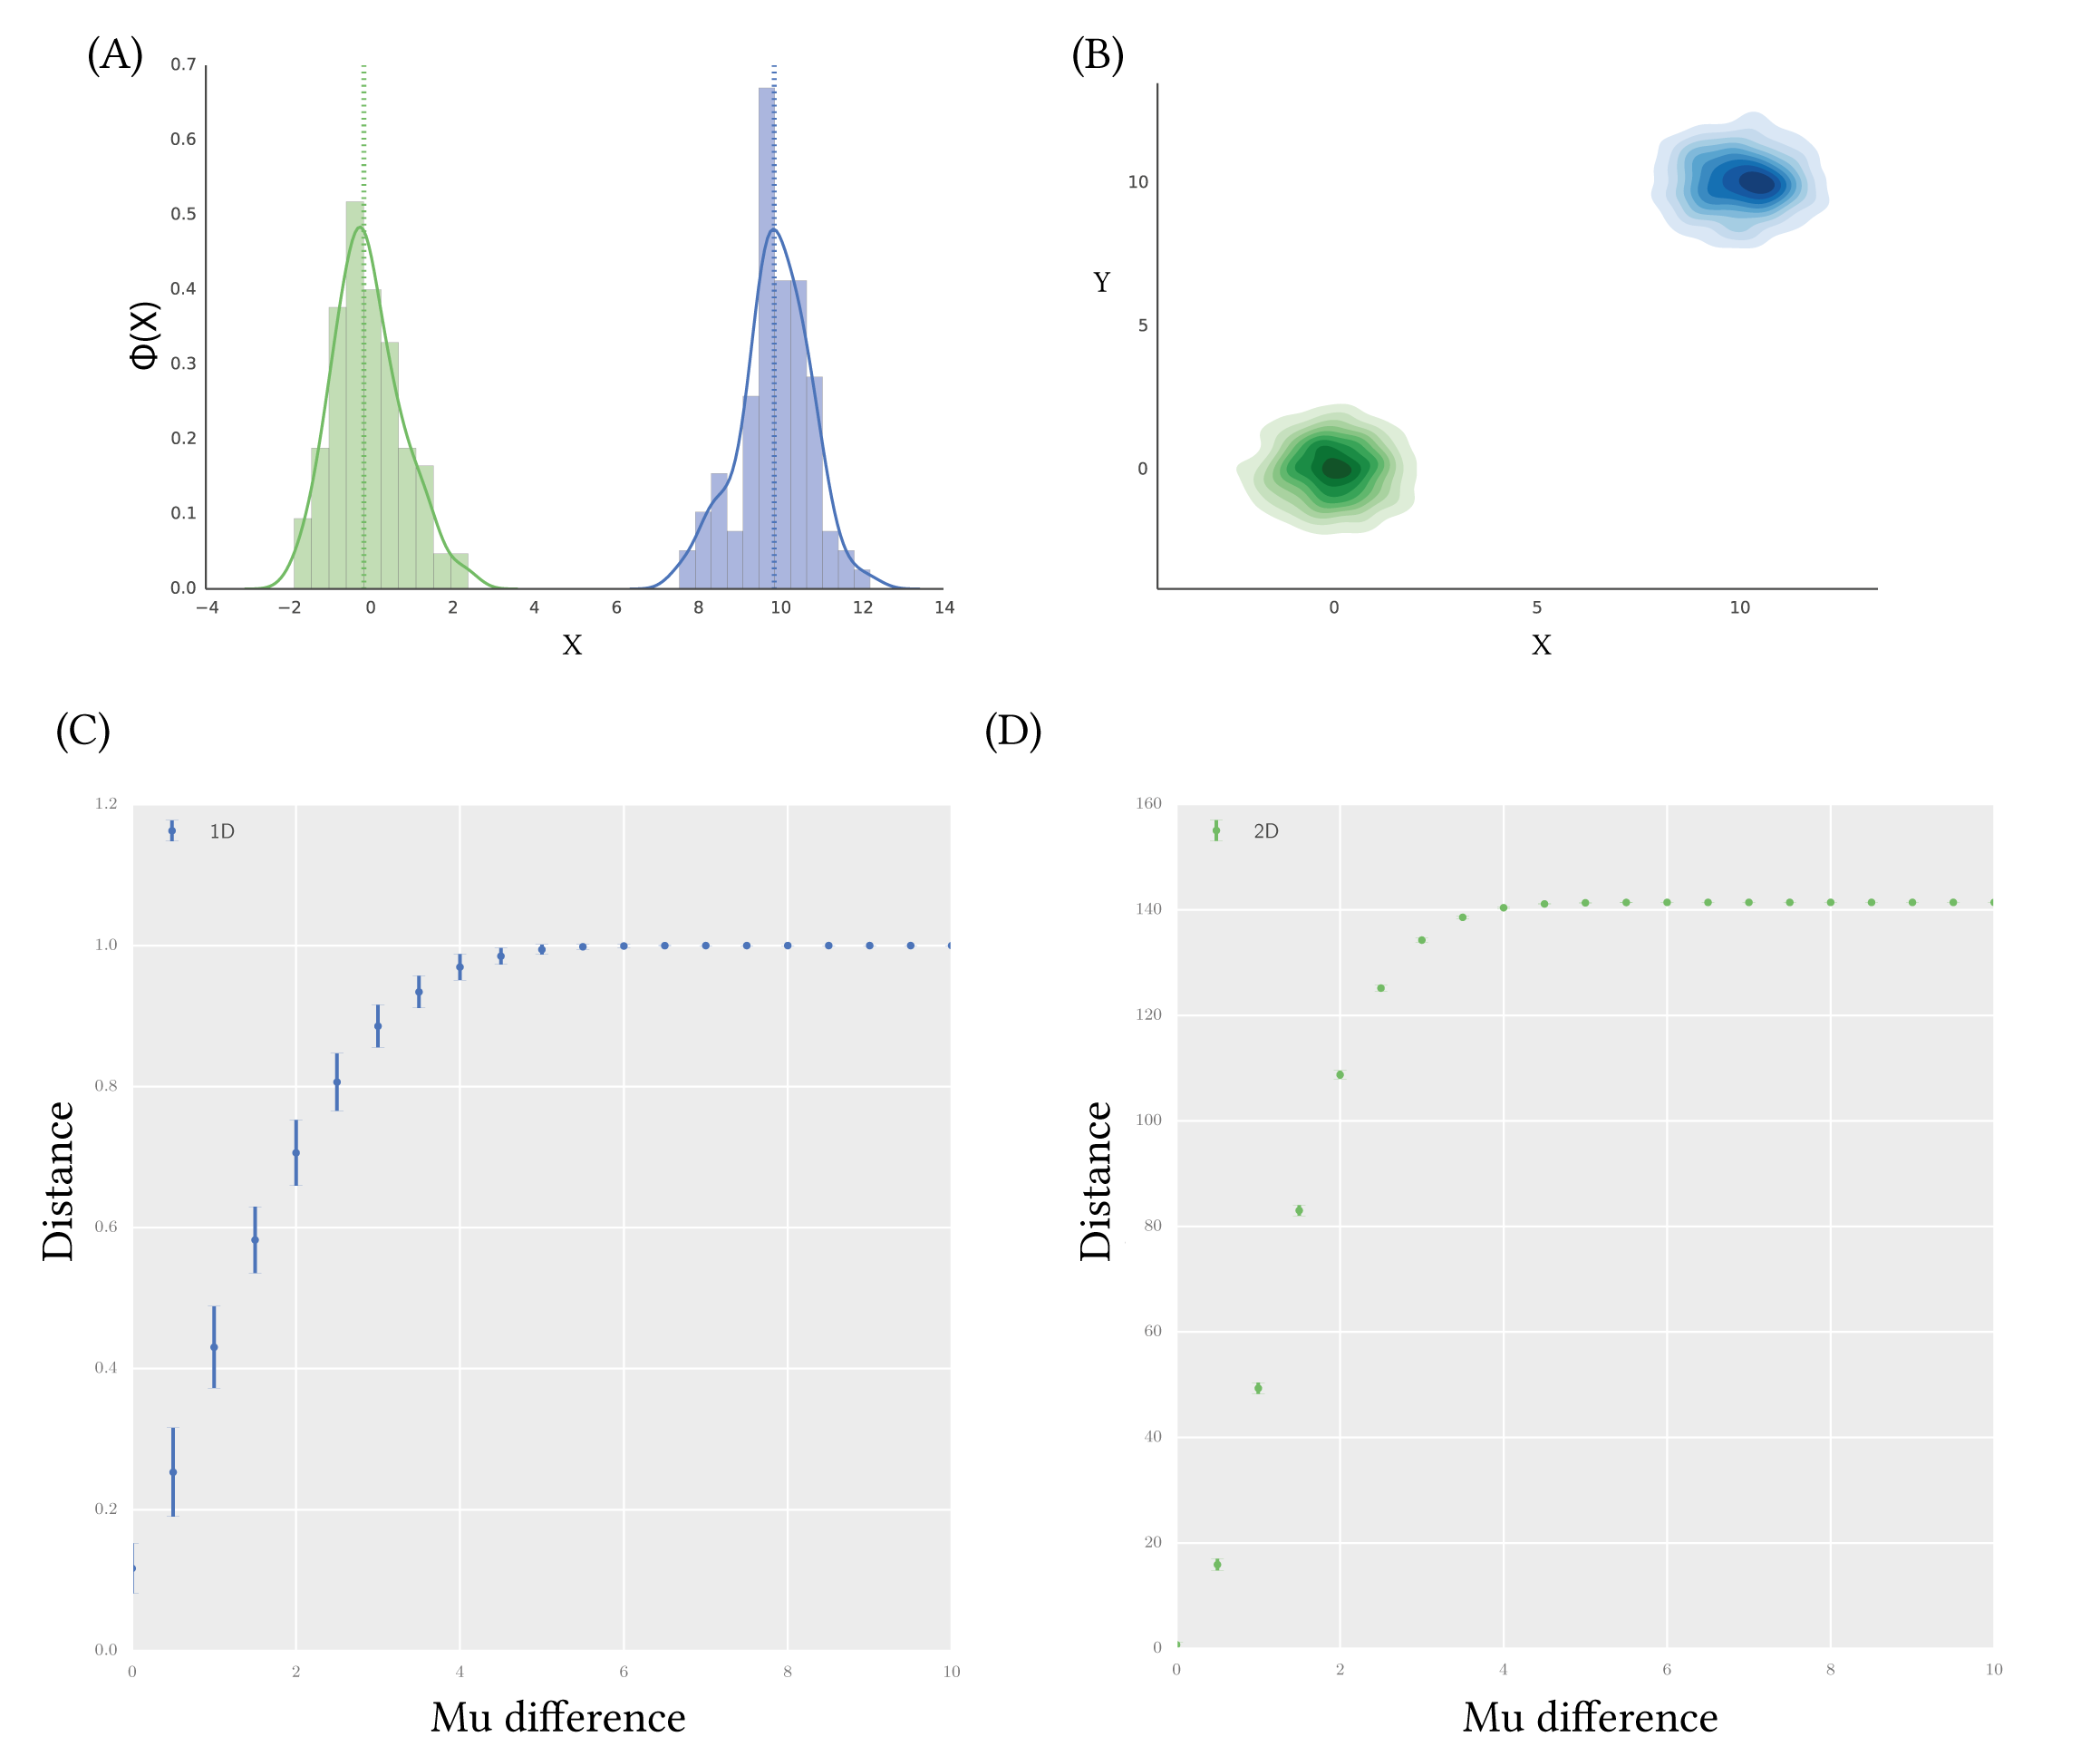
\includegraphics[scale=0.8]{../../chapters/chapterABCFlow/images/mu_diff.png}
\caption[Range of distance values obtained using the Wald-Wolfowitz distance]{\label{fig:epsilon_mud}The distance calculation for data sets drawn from increasingly different distributions. Two examples are shown of distributions compared in (A) 1D and (B) 2D. (C) As the difference between the means of the two 1D distributions increases, the KS distance calculation increases until it plateaus at 1. (D) In the 2D case the distance plateaus at 140.}
\label{fig:normal_example}
\end{figure}


\begin{figure}[tb]
\centering
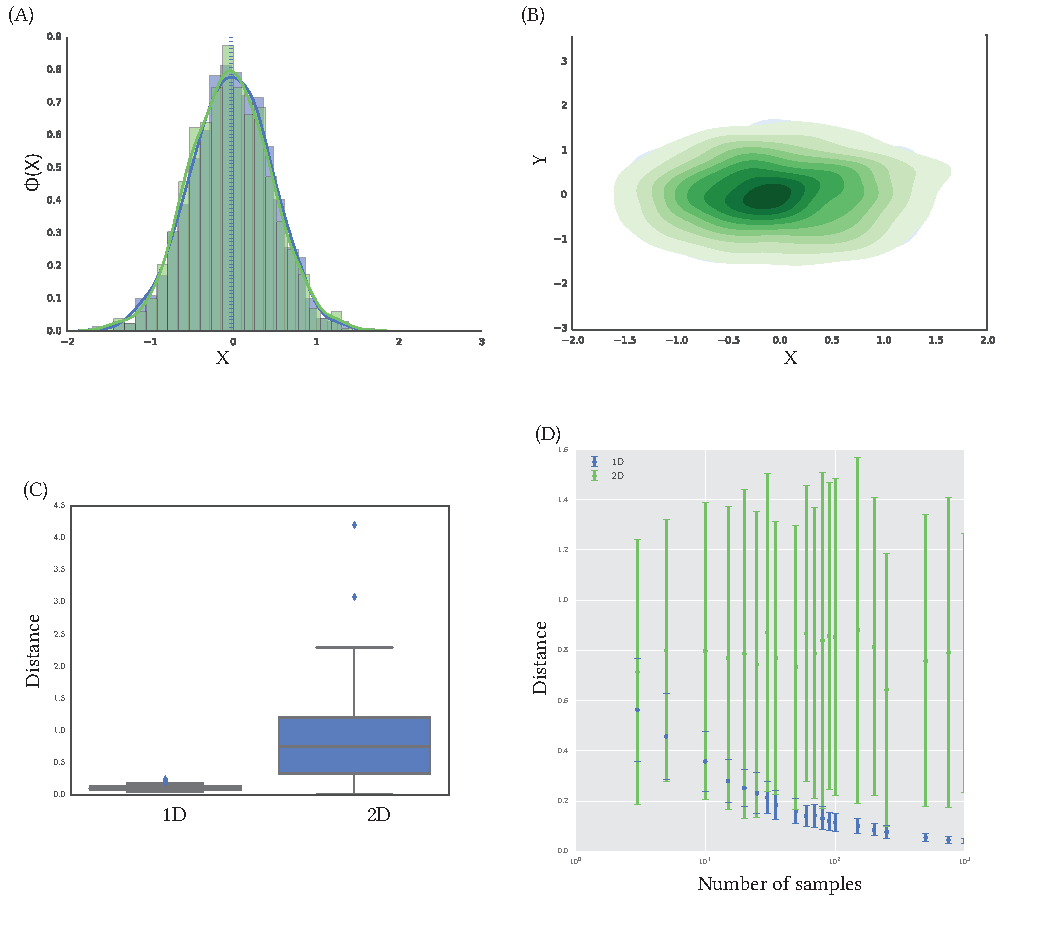
\includegraphics[scale=0.7]{../../chapters/chapterABCFlow/images/epsilon_same_box.pdf}
\caption[Distance calculation expected error using the KS and Wald-Wolfowitz distances]{\label{fig:epsilon_boxplt}The distance between two data sets drawn from the same distribution are compared using (A) the Kolmogorov-Smirnov in 1D and (B) the Wald-Wolfowitz distance in 2D. (C) The distance is calculated for 1000 data sets. A larger variation of values is found for the 2D distance calculation, but still small relative to the overall range of values that the 2D distance can take. (D) As the number of samples in the datasets increase the distance calculation becomes more accurate in the 1D case. It has no effect on the 2D case.}
\end{figure}


Using the Wald-Wolfowitz test the distance value increased with increasing distance between the distributions with relatively small variability between repeats. Since the 2D Wald-Wolfowitz test performed well in the test carried out above, it was implemented in ABC-Flow as the distance function for the 2D calculations.
%The next parameter to be optimised is the bin size used in the distance calculation. In both 1D and 2D, the space is divided into bins, and the distance between corresponding bins in the data and the simulated data is calculated. The overall distance between to distributions is the sum of the distances between corresponding bins. %If the bin size is too large, small differences between 


%We find that the 2D distance is more sensitive to the bin size than the 1D distance. From Figure~\ref{fig:epsilon_ngrid} we conclude that for a sample size of 100 data points, the optimal bin size for 1D and 2D distance calculation is 10. The above optimizations have been made by using standard normal distributions, of $\mu=0$ and $\sigma=1$. Here we investigate whether the distance calculation depends on the $\mu$ and $sigma$ of the distributions. 

%Next, by varying the amount of $\mu$ and $\sigma$ by which the two normals differ, we can find out the dynamical range of the epsilons. Whether two distributions are identical or vary by a large amount, we can get an estimate of how much the epsilon will vary from one to the other, both in 1D and 2D. 


%From Figure~\ref{fig:epsilon_mu_s_diff} we find that as the difference in $\mu$ increases the epsilon medians reach a plateau. We find that beyond a difference of 4 in $\mu$, the distance calculation cannot further separate the distances. This can be caused by the fact that when first dividing the space into bins, the range of the data is used to define the grid. If all the simulated data is located outside that grid, the algorithm can no longer distinguish between them, and will only allocate them as outside the range. The variance of the epsilon distributions does not vary significantly with increasing difference in $\mu$. As the difference in $\sigma$ increases between the distributions, we find that the median in the 2D distance calculation increases but not in the 1D. Note, that the range of the difference in the epsilon medians is small and thus we conclude that differences in the $\mu$ of a distribution are much better detected than the differences in the $\sigma$. The variance of the epsilon distribution when $\sigma$ is varied does not change significantly with increasing $\sigma$ difference.


%We study the epsilon distribution variance in the uniform distribution, [0, 1].  
%When comparing a normally distributed data set to a uniformly distributed data set, we don't see a great difference between the 1D and 2D epsilons.


%Another type of distribution that is commonly found in Flow cytometry experiments, is a bimodal distribution. Here we test whether the 1D and 2D distances are equivalent when measuring distances in this type of distributions.


%Finally, we study how the distances perform when comparing a bimodal with a normal distribution. We test the distances by using a bimodal distribution and a series of normal distributions with increasing $\mu$, in 1D and 2D. We find that epsilon is the lowest when the $\mu$ of the normal distribution corresponds to the $\mu$ of one of the two peaks in the bimodal distribution and the highest when there is no overlap between the distributions. 





%The following is for 1D, what about for 2D?????
%As determined by~\textcite{Lillacci:2011tqa} and~\textcite{Lillacci:2013hu}, the minimum number of samples that are necessary in order to accurately compare the two distributions decreases with increasing number of samples in the flow cytometry data. Typically a flow cytometry experiment includes thousands of samples, and thus the number of simulations needed to assess whether the two distributions are the same is small. The number of simulated samples S can be calculated using Equation~\ref{eq:Samples}. 
%
%\begin{align}
%	S \geq \frac{-\log(\frac{α}{2})}{2\Bigg(ε-\sqrt{-\frac{1}{2M}\log(\frac{α}{2}) } \Bigg)^2}\label{eq:Samples}, 
%\end{align}
%
%where $α = 1 - \sqrt{1 - β} $, β represent the confidence interval (here set to 0.05) M is the number of samples of the data and ε is the critical value. This allows us to determine the number of samples needed to accurately calculate the KS distance. For a typical experiment including 10000 samples, with a confidence interval of 0.05 and an ε of 0.08, 514 simulated samples are needed (rounded to the nearest integer). This is defined in ABC-Flow by beta, the number of simulations to be made per parameter sample. This value has to be set to at least 500 in order to get an accurate calculation of the distance. Since the ε value is iteratively decreased in ABC-Flow, the I set beta to satisfy Equation~\ref{eq:Samples} for the lowest ε.
\clearpage
\section{ABC-Flow model fitting to simulated data }


%section{ABC-Flow validation using simulated data}

In this section I apply ABC-Flow to simulated data, where the parameter values used to produce the data are known. This analysis will serve as a verification test for ABC-Flow. 

\subsection{Toggle switch model development}
The model used to produce the simulated data is an extension of the~\textcite{Gardner:2000vha} switch. The model consists of two mutually repressing transcription factors. The model used here has additional parameters allowing for gene expression to be leaky as well as include repression from an external stimulus. In order to produce the data set the model was simulated stochastically using the Gillespie algorithm~\autocite{Gillespie:1977ww}. The model used is defined by the following hazards:

\begin{align}
h_1 &= u \label{eq:eg1}\\
h_2 &= \frac{a_1  l_1	}{1+l_1+v^{β}} \label{eq:eg2}\\
h_3 &= (1 + α) v \label{eq:eg3}\\
h_4 &= \frac{a_2 l_2}{1+l_2+u^{γ}} \label{eq:eg4},
\end{align}
\noindent where $u$ and $v$ are the two proteins in the system, $a_1$ and $a_2$ represent the effective gene expression of $u$ and $v$ respectively, $β$ and $γ$ represent the cooperativity of $u$ and $v$ respectively and $l_1$ and $l_2$ represent the leakiness of the promoters for each species. Parameter α represents the addition of an inducer molecule that binds to repressor $v$, effectively increasing its degradation. This has been used previously to successfully represent the addition of the IPTG repressor to the system~\autocite{Lillacci:2013hu}.

In addition, the system included a fluorescence intensity model. Each fluorescent molecule was assumed to emit a fluorescent signal and the signal was assumed to be normally distributed around a mean μ and standard deviation σ. The fluorescent signal emitted by each molecule was described using Equation~\ref{eq:intens}. There was also a background fluorescence signal added to each calculation. This represents the intensity signal detected by flow cytometers when no fluorescent proteins are present~\autocite{Lillacci:2013hu}. The background fluorescence can be measured using control samples~\autocite{Lillacci:2013hu}, but in the case of the simulated data it was set to 0.01 (a.u.).  


\begin{table}[tb]
\centering
\caption{The priors used for the 1D and 2D ABC-Flow model fitting to simulated data}
\label{tab:priors_model}

\begin{tabular}{@{}ccc@{}}
\toprule
\multicolumn{3}{c}{Parameters}                                         \\ \midrule
\multicolumn{1}{c}{} & \multicolumn{1}{c}{1D} & \multicolumn{1}{c}{2D} \\ \midrule
a\textsubscript{1}                   & 80 - 120               & 80 - 120               \\
β                   & 1 - 4                  & 1 - 4                  \\
l\textsubscript{1}                  & 750 - 850              & 750 - 850              \\
a\textsubscript{2}                  & 80 - 120               & 80 - 120               \\
γ                   & 1 - 5                  & 1 - 4                  \\
l\textsubscript{2}                   & 750 - 850              & 750 - 850              \\
α                   & 1 - 4                  & 1 - 4                  \\ \midrule
\multicolumn{3}{c}{Species}                                            \\ \midrule
u                    & 9 - 11                 & 9 - 11                 \\
v                    & 90 - 110               & 90 - 110               \\ \midrule
\multicolumn{3}{c}{Intensity parameters}                               \\ \midrule
μ fp\textsubscript{u}             & 0 - 2                  & 0 - 2                  \\
μ fp\textsubscript{v}             &                   & 0 - 2                  \\
σ fp\textsubscript{u}            & 4 - 6                  & 4 - 6                  \\
σ fp\textsubscript{v}            &                   & 4 - 6                  \\ \bottomrule
\end{tabular}

\end{table}




\subsection{Parameter inference for simulated flow cytometry data}

The model given in Equations~\ref{eq:eg1}-\ref{eq:eg4} was simulated in order to obtain the time course for the two fluoscent molecules in the system, $u$ and $v$. The  time course data, the model and the prior distributions shown in Table~\ref{tab:priors_model} were supplied to ABC-Flow. ABC-Flow was then used to infer the parameters that gave rise to the data using one (1D) or both (2D) fluorescent molecule time courses to fit to the data. We can therefore determine whether there is an added benefit on fitting both fluorescent proteins to the data. In order to compare the 1D and 2D fits, equivalent epsilon distance values were used. These were set to 0.27 for the 1D fit and 2.82 for the 2D fit.

The fit resulting from the 1D fit is shown in Figure~\ref{fig:1d-sim-res}A, together with Q-Q plots to assess the fit to the data. A Q-Qplot is a plot where the quantiles of two distributions are plotted against each other. If the distributions are the same then the points will lie on the x = y line~\autocite{Wilk:1968ts}. The fit resulting from the 2D fit is shown in Figure~\ref{fig:2d-sim-res}, while the posterior distributions obtained from both fits are shown in Figure~\ref{fig:1d2d-sim-post} and Table~\ref{tab:inf_params_sim}. Comparing the 1D and 2D fits, we find that both fits inferred the parameters necessary to produce the simulated data. From the posteriors we find that the most identifiable parameters in this model are parameters $β$ and $γ$, the parameters representing the cooperativity of the repressors. We find that the 2D fit resulted in a better inference of the parameter values. This is most prominent in parameters $β$, $γ$ and $α$ as can be seen in Table~\ref{tab:inf_params_sim}. Parameters $a2$ and $l2$ remained unidentifiable for both fits. For a system involving two fluorescent proteins, like the toggle switch, it would therefore be beneficial to use a two-dimensional fit to the data. The 2D fit performed better in the simulated test used here, with priors centred closely around known parameter values and clean data. This will become more evident when ABC-Flow is used on real experimental data where less information is known for the priors. Furthermore, the 1D fits do not fit intensity parameters for the both fluorescent proteins. This means that the 2D time course of the model using inferred parameters cannot be examined to assess the fit for both proteins. Therefore, a system involving two fluorescent proteins should be fit using the 2D fit in ABC-Flow. The 1D fit should be used in cases where there is only one fluorescent protein of interest in the system. 

%By examining the data and the fitted models shown in Figure~\ref{fig:1d-sim-res}, we see that at ε = 0.27, there is a good fit of the model to the data using ABC-Flow. The model parameters, as well as the intensity parameters, have been fitted to simulated flow cytometry data. This is highlighted in the QQ plots in Figure~\ref{fig:1d-sim-res}B, where the results lie in the x=y line. 

\begin{figure}[htbp]
\centering
	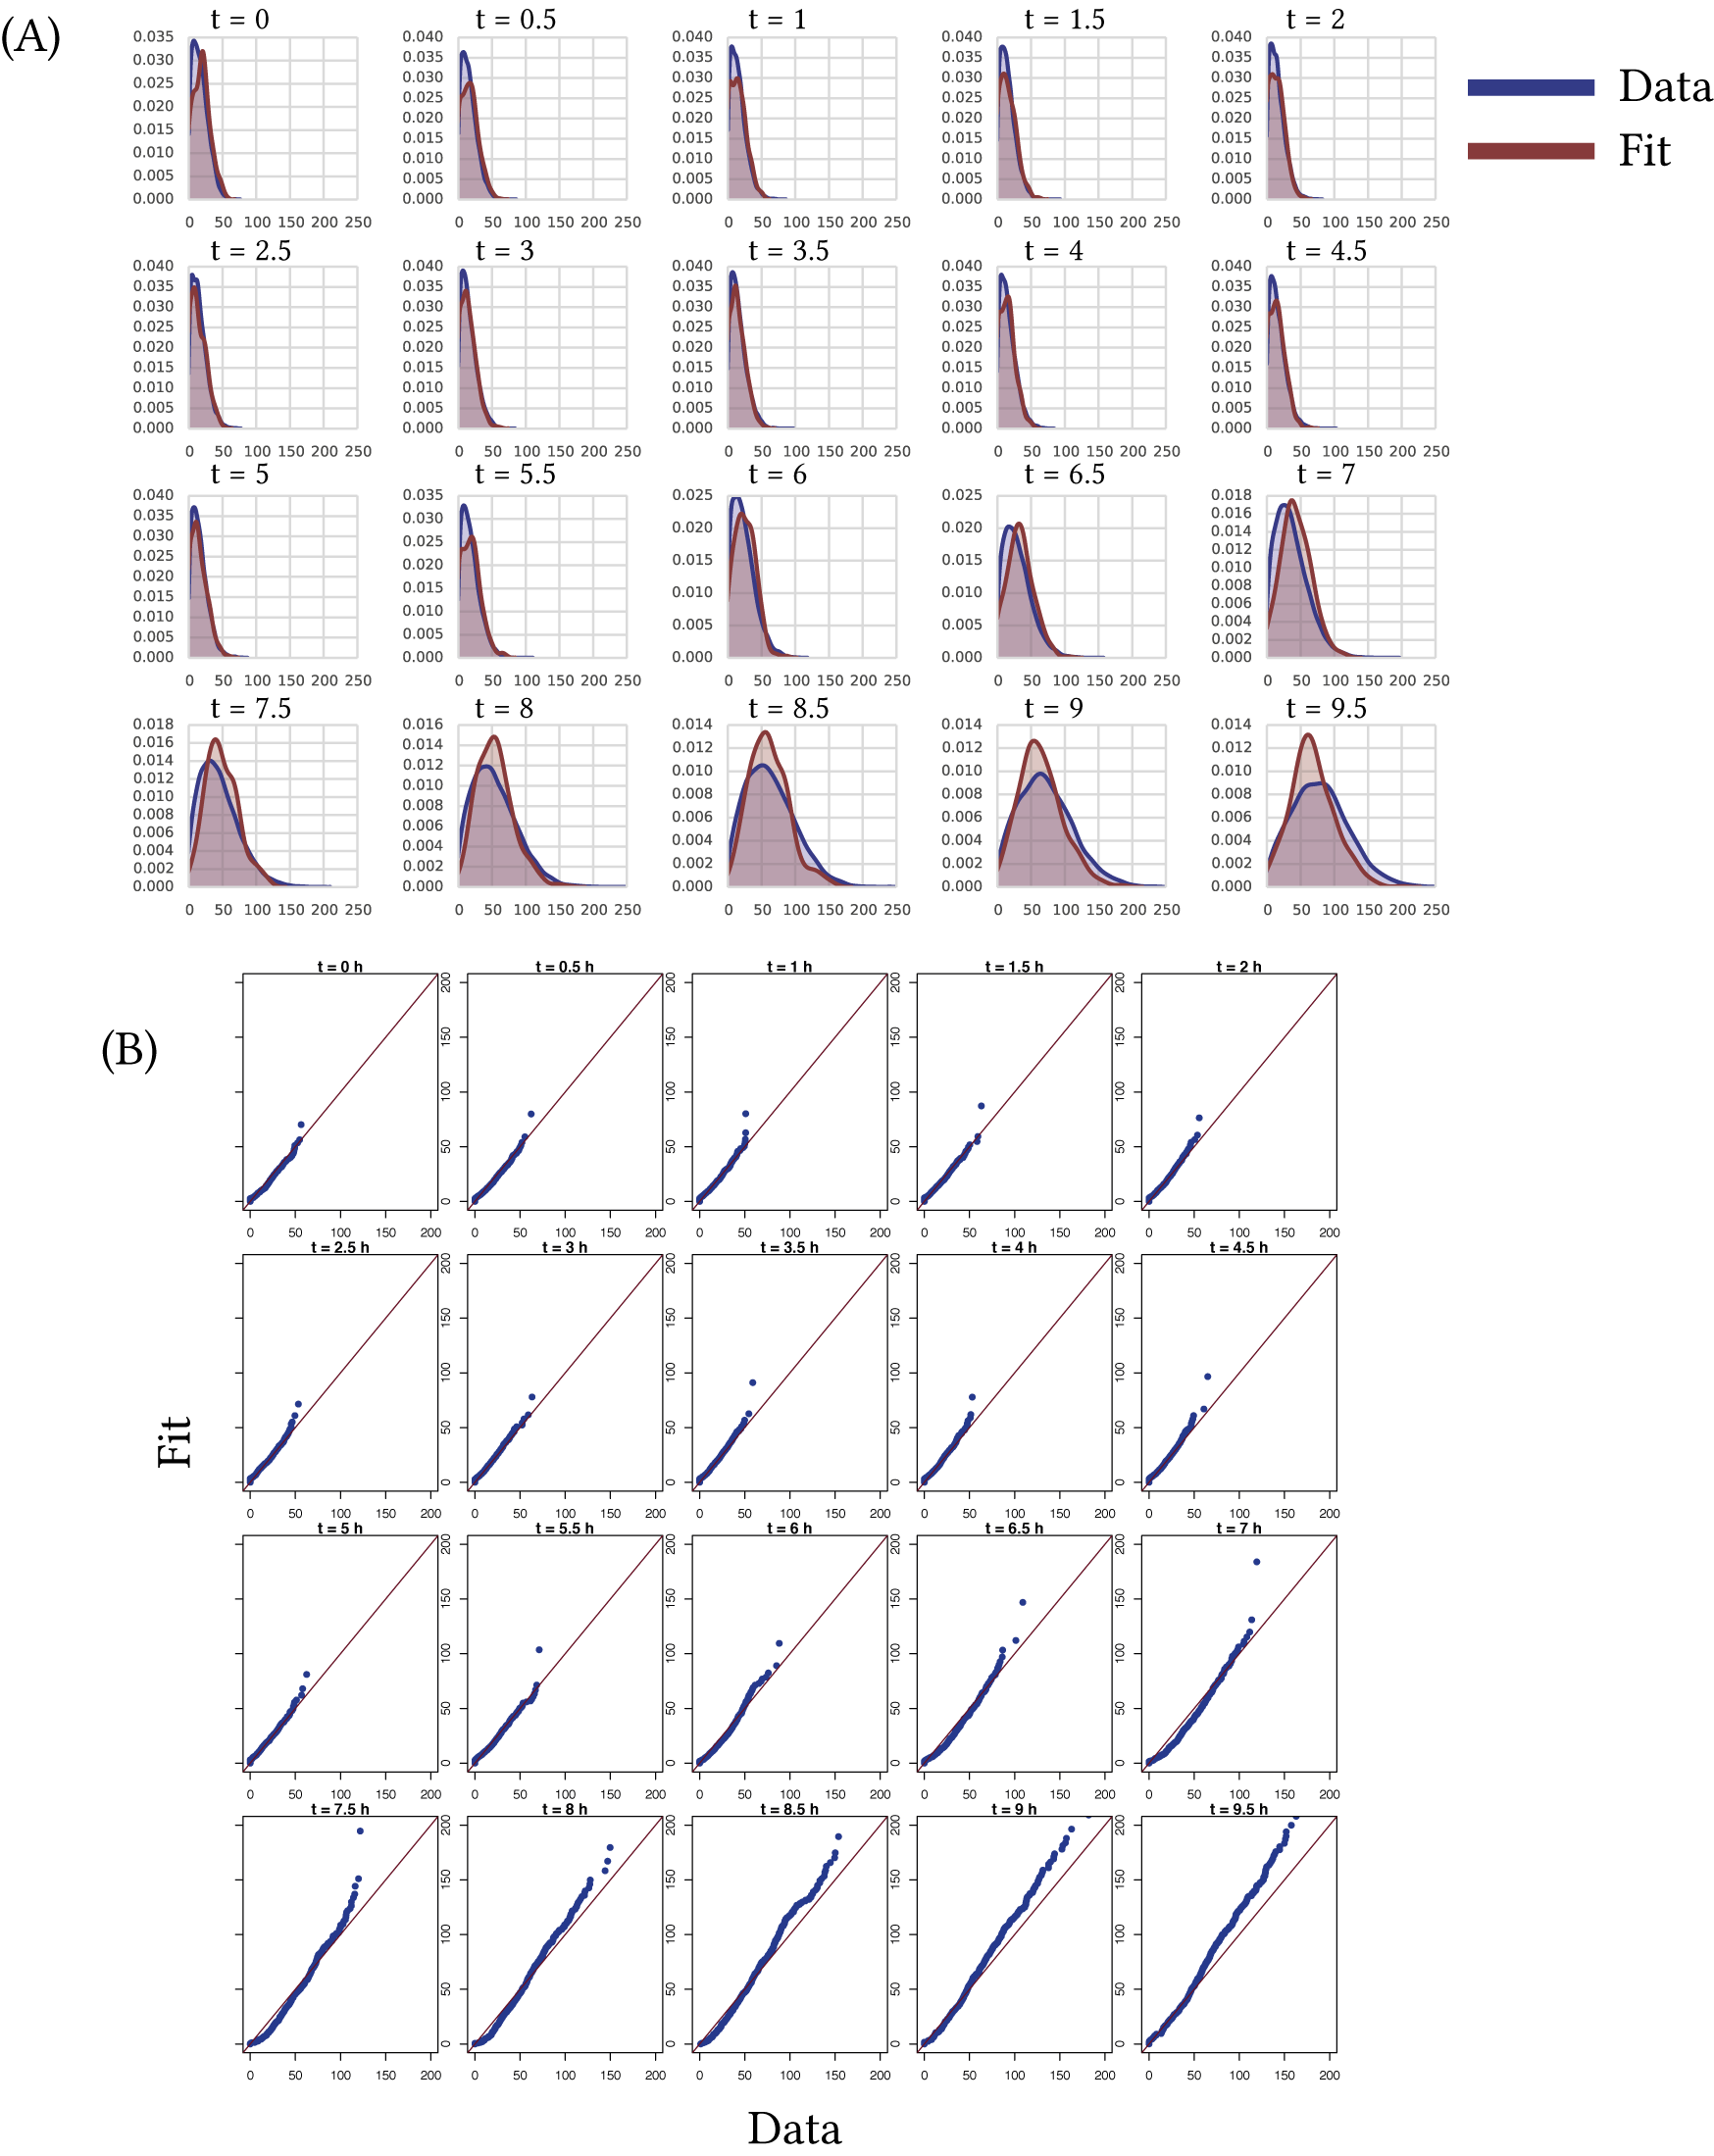
\includegraphics[scale=0.9]{../../chapters/chapterABCFlow/images/1D_sim_res.png}
	\caption[ABC-Flow parameter inference for 1D simulated data]{\label{fig:1d-sim-res} (A) Time course produced by the 1D ABC-Flow fit (shown in blue) to data (shown in red) produced by simulating the same model. (B) Q-Qplot of each time point fit. The quantile of the two distributions are plotted against each other. If the distributions are identical, the points would lie on the x = y line, shown in red. }
\end{figure}






%We also find that α, the parameter representing the increased degradation of $v$ due to the addition of an inducer, is well inferred. %Further, we find μ and σ, the parameters representing the mean and standard deviation of the fluorescence intensity emitted by each fluorescent molecule to be inferred well.

\begin{figure}[htbp]
\centering
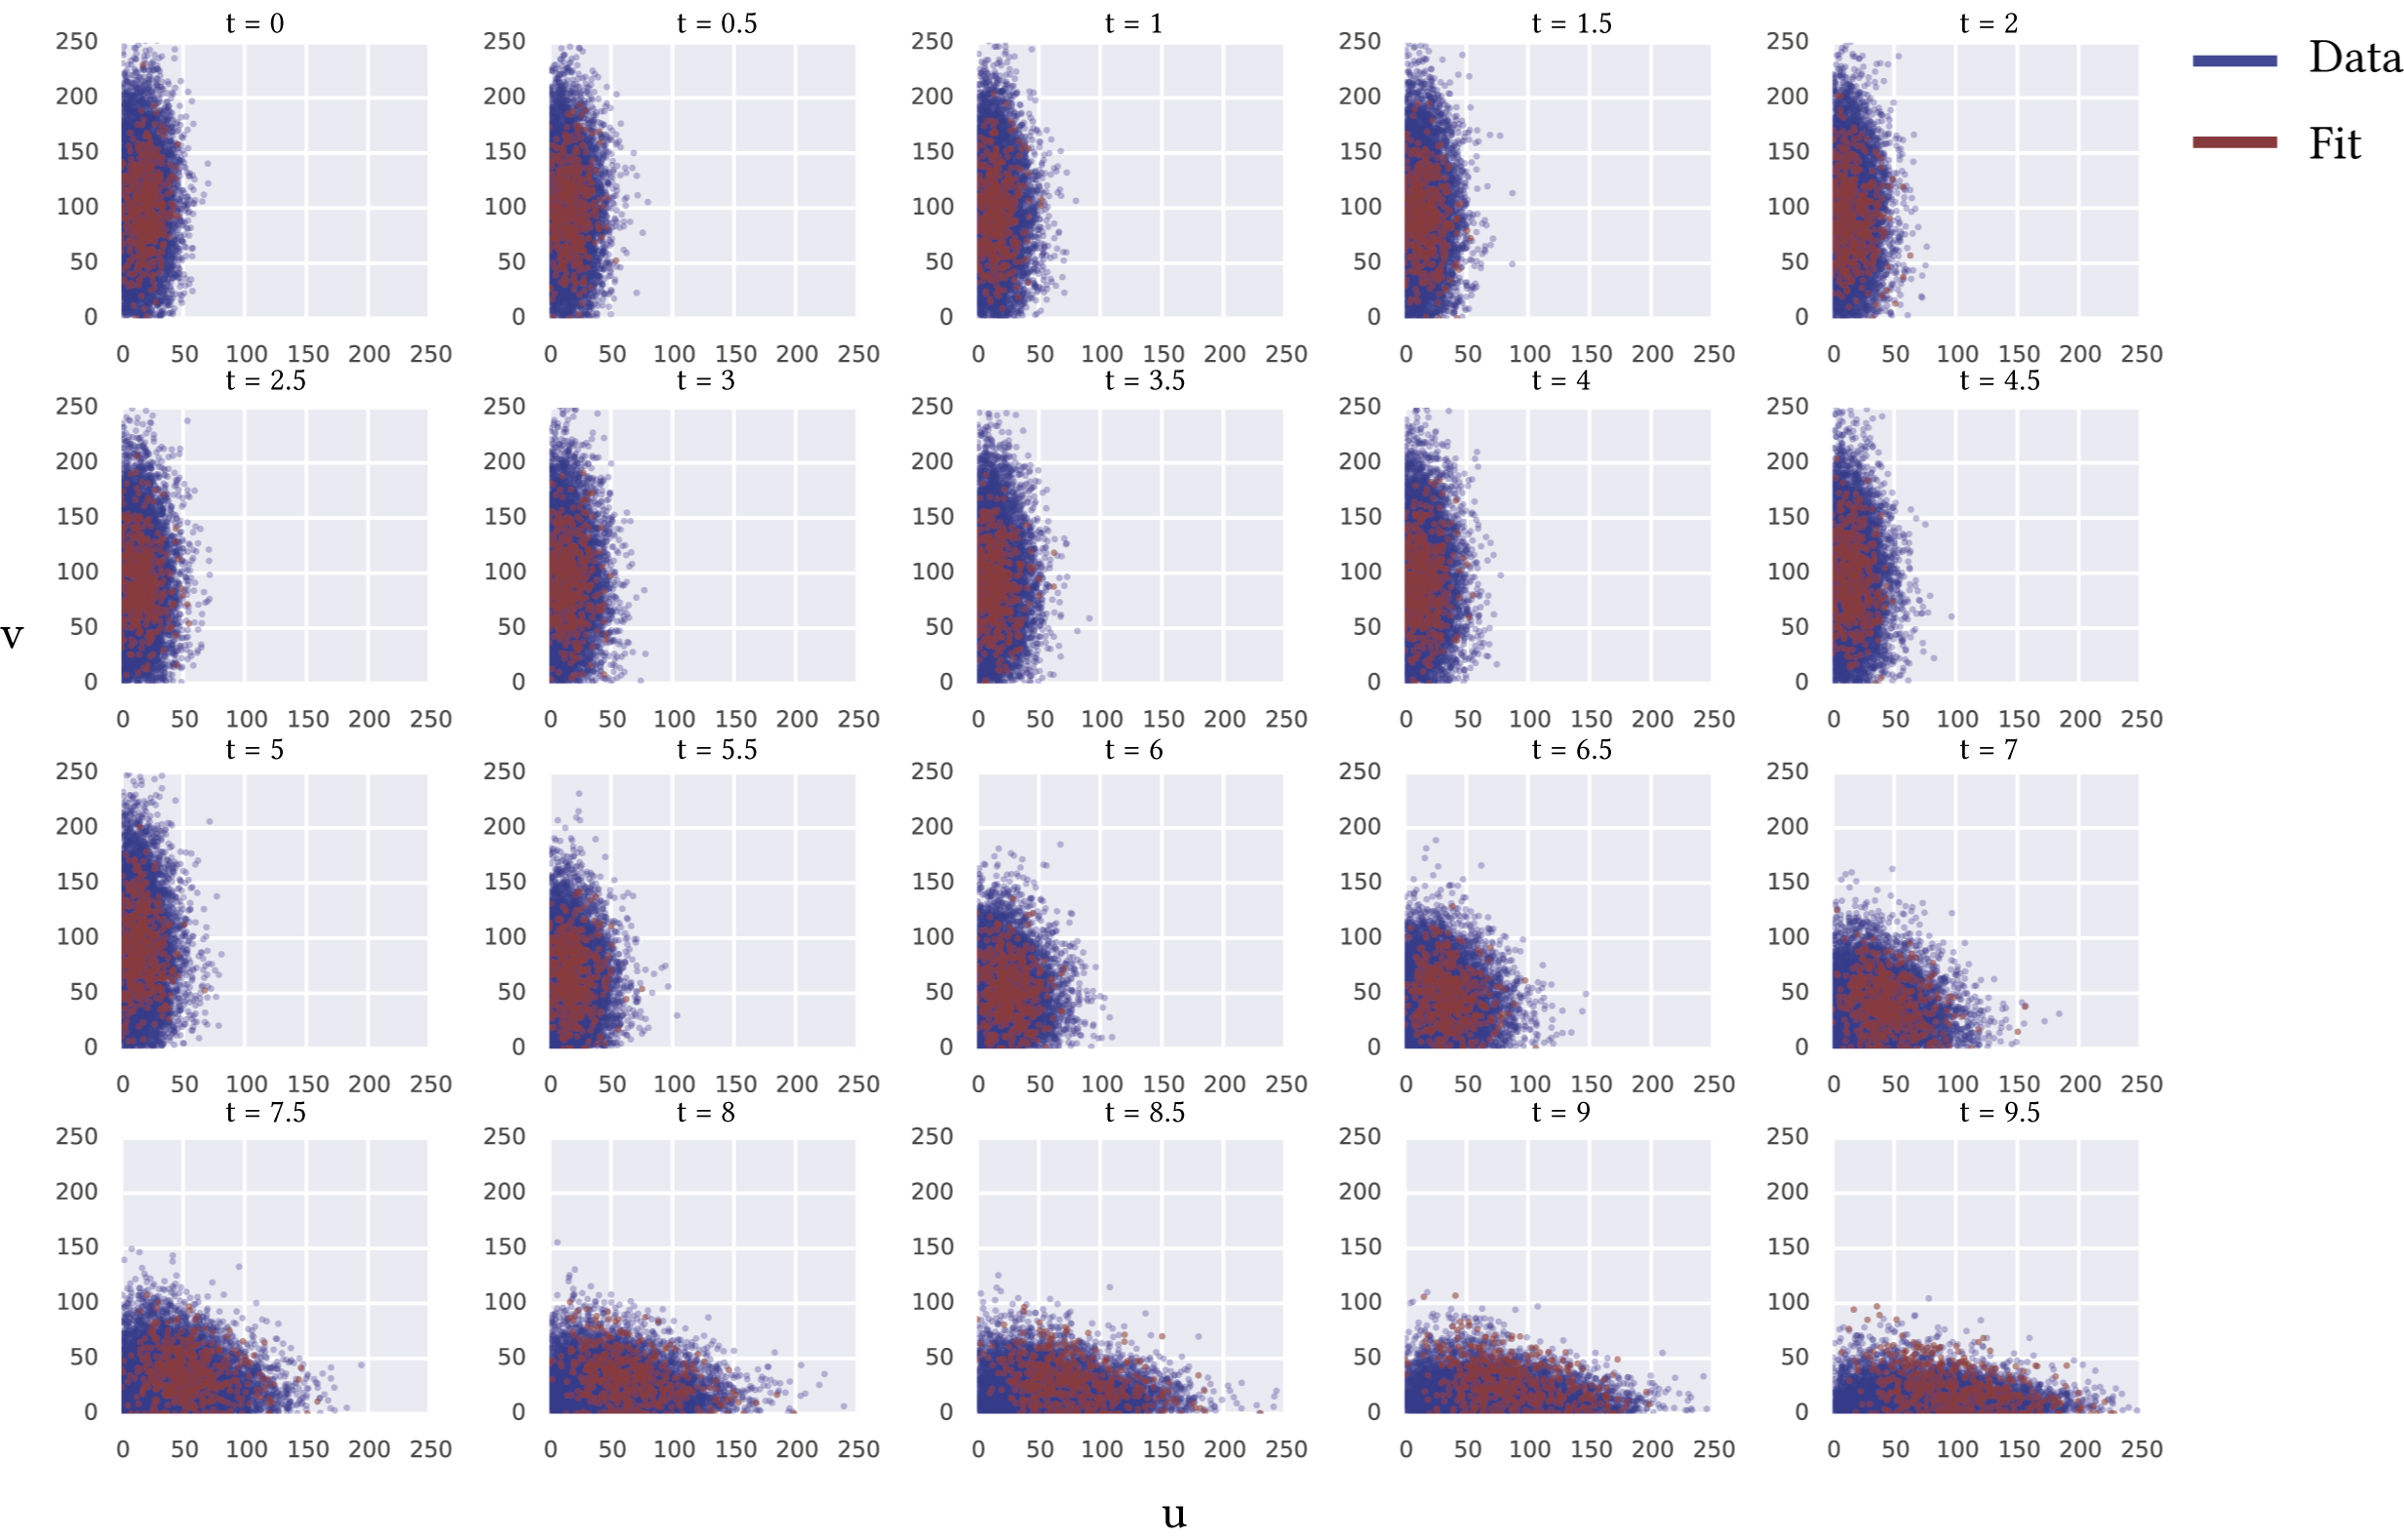
\includegraphics[scale=0.7]{../../chapters/chapterABCFlow/images/2D_flow_time.png}
\caption[ABC-Flow parameter inference for 2D simulated data]{\label{fig:2d-sim-res}2D ABC-Flow fit (shown in blue) to data (shown in red) produced by simulating the same model. }
\end{figure}

%
%I further investigate whether using the 1D or 2D data results in a better fit. The 1D data represents one of the marginal distributions of the data sets. I use the marginal distribution of $u$ and the bivariate distribution of $u$ and $v$ in order to determine which one produces a better fit to the data. The resulting timecourse of the data as well as the 1D and 2D fit are shown in Figure~\ref{fig:1d2dcomp}.
%
%
%\begin{figure}[htbp]
%\centering
%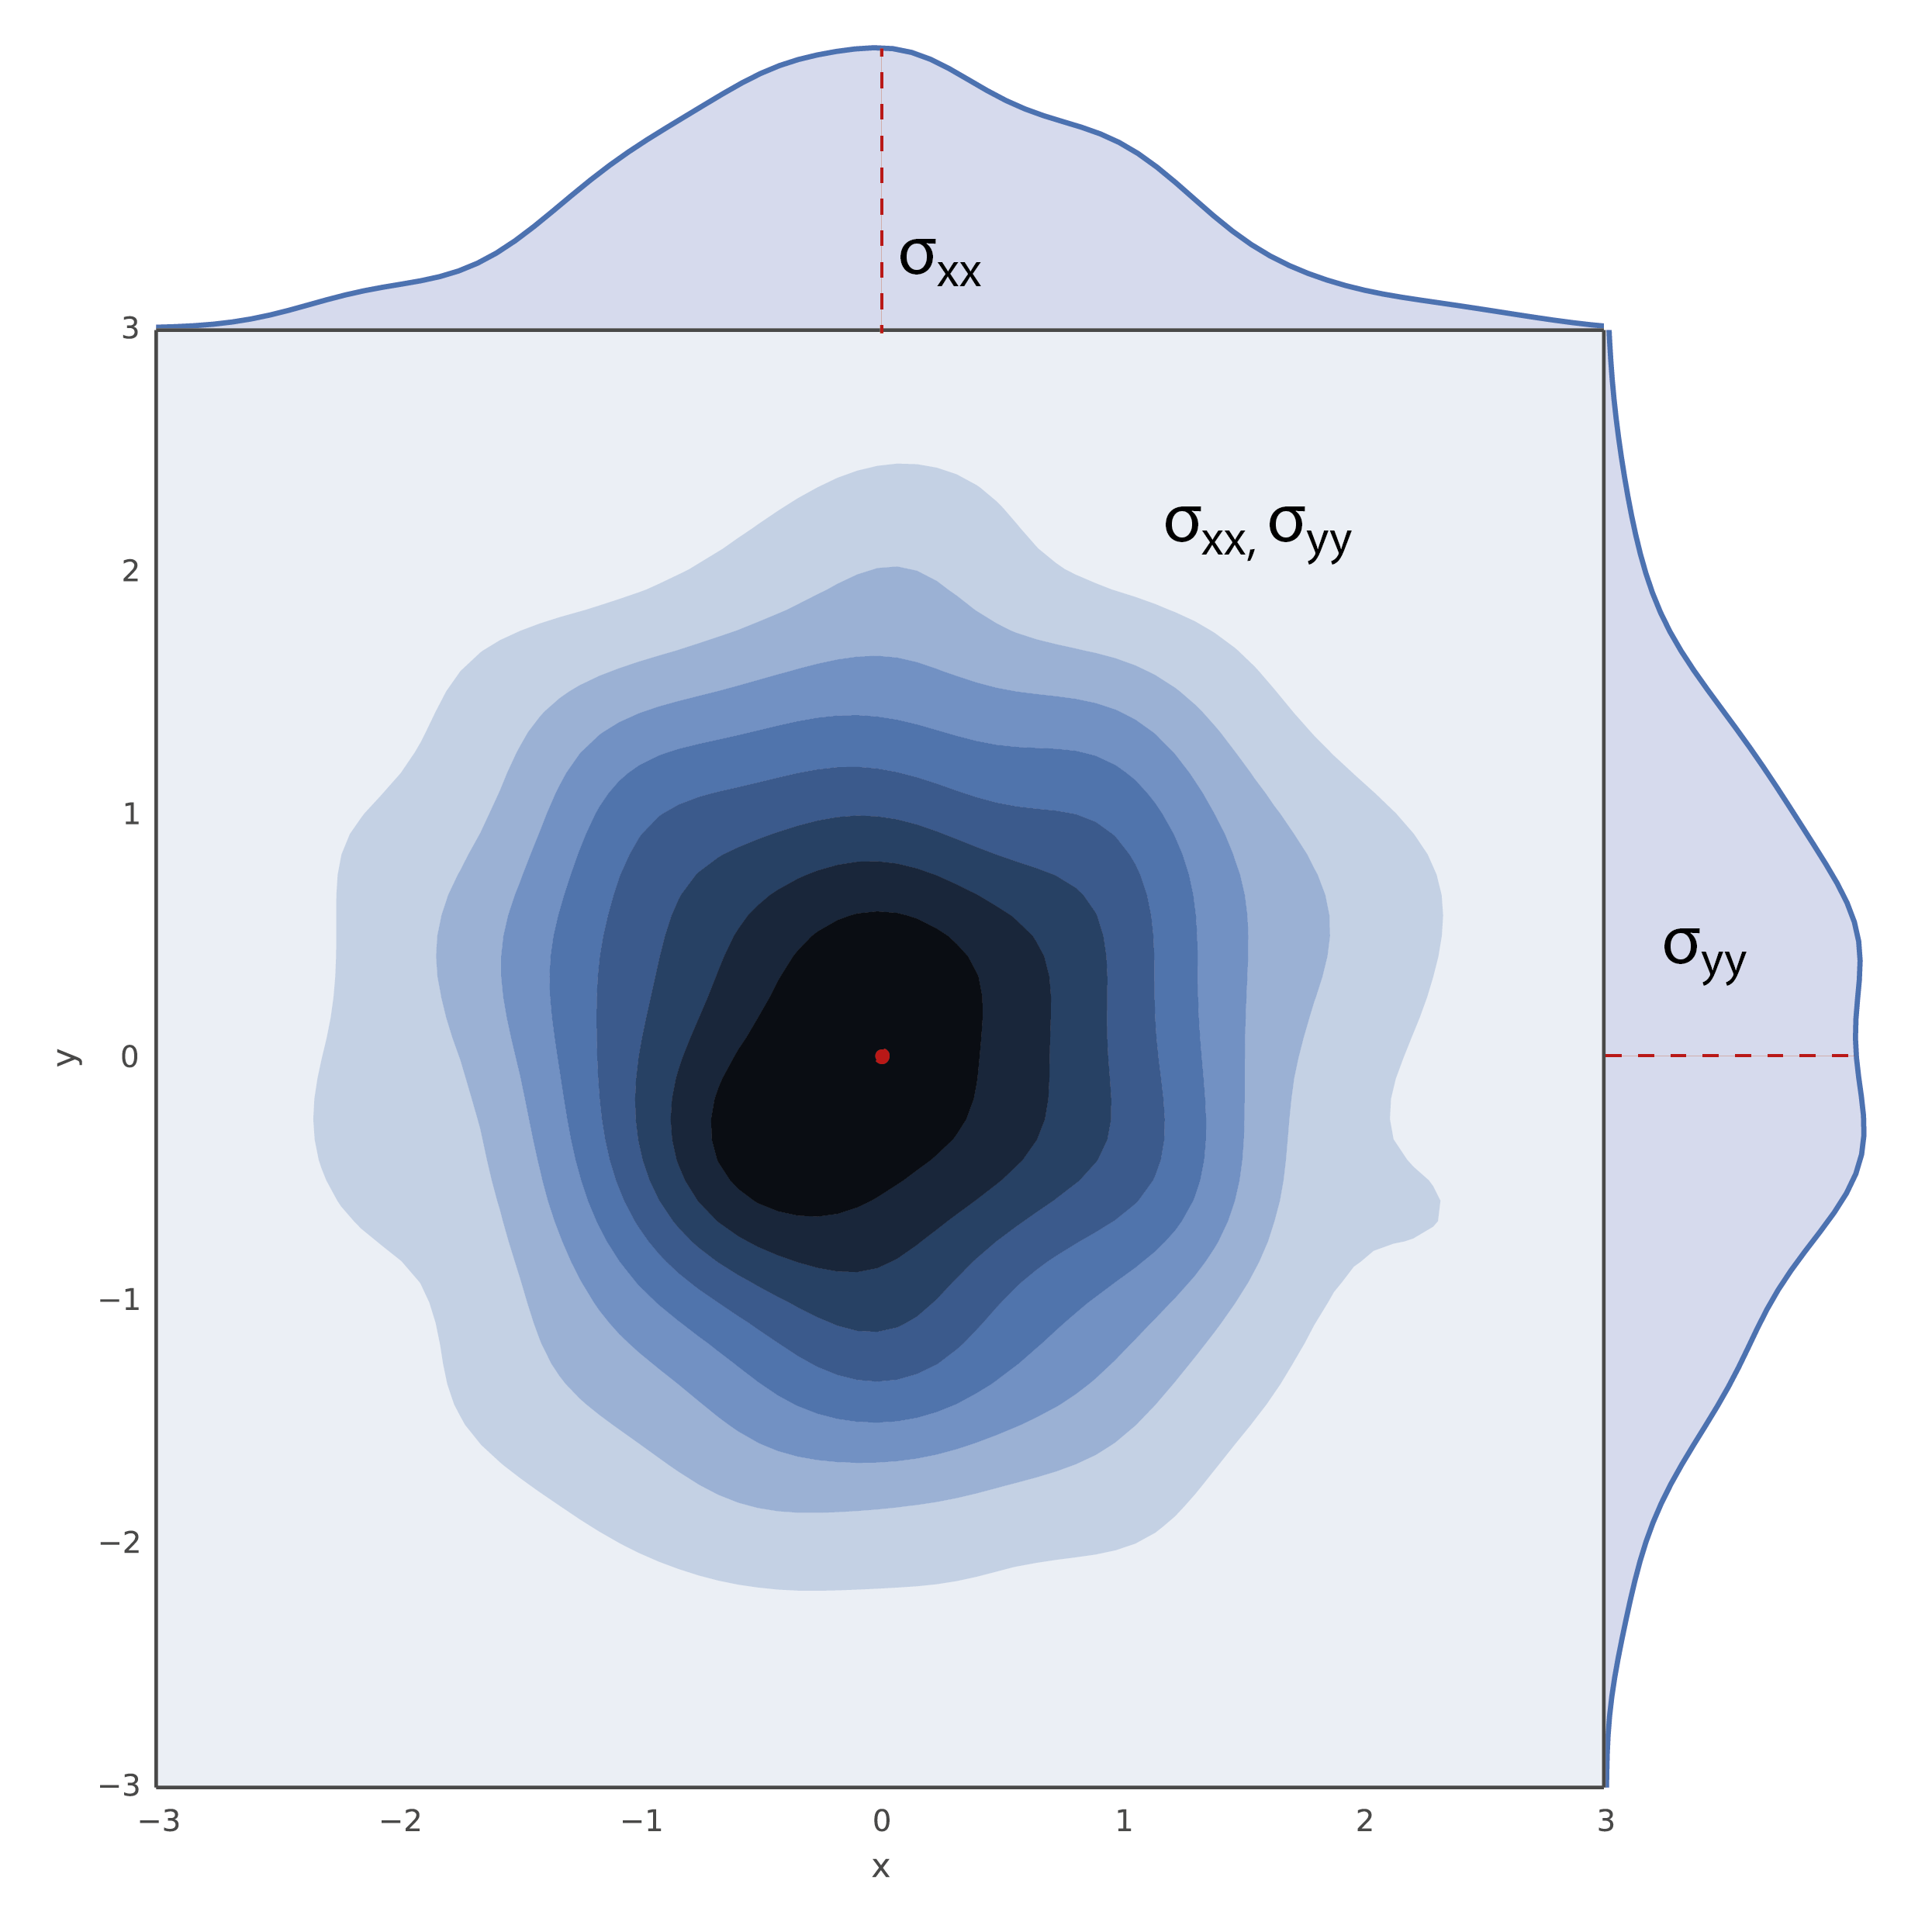
\includegraphics[scale=0.3]{../../chapters/chapterABCFlow/images/normal_sigma_example.png}
%\caption[LoF caption]{\label{fig:1d2dsketch} The marginal (1D) versus the bivariate (2D) distribution of the data.}
%\end{figure}
%



%\begin{figure}[htbp]
%\centering
%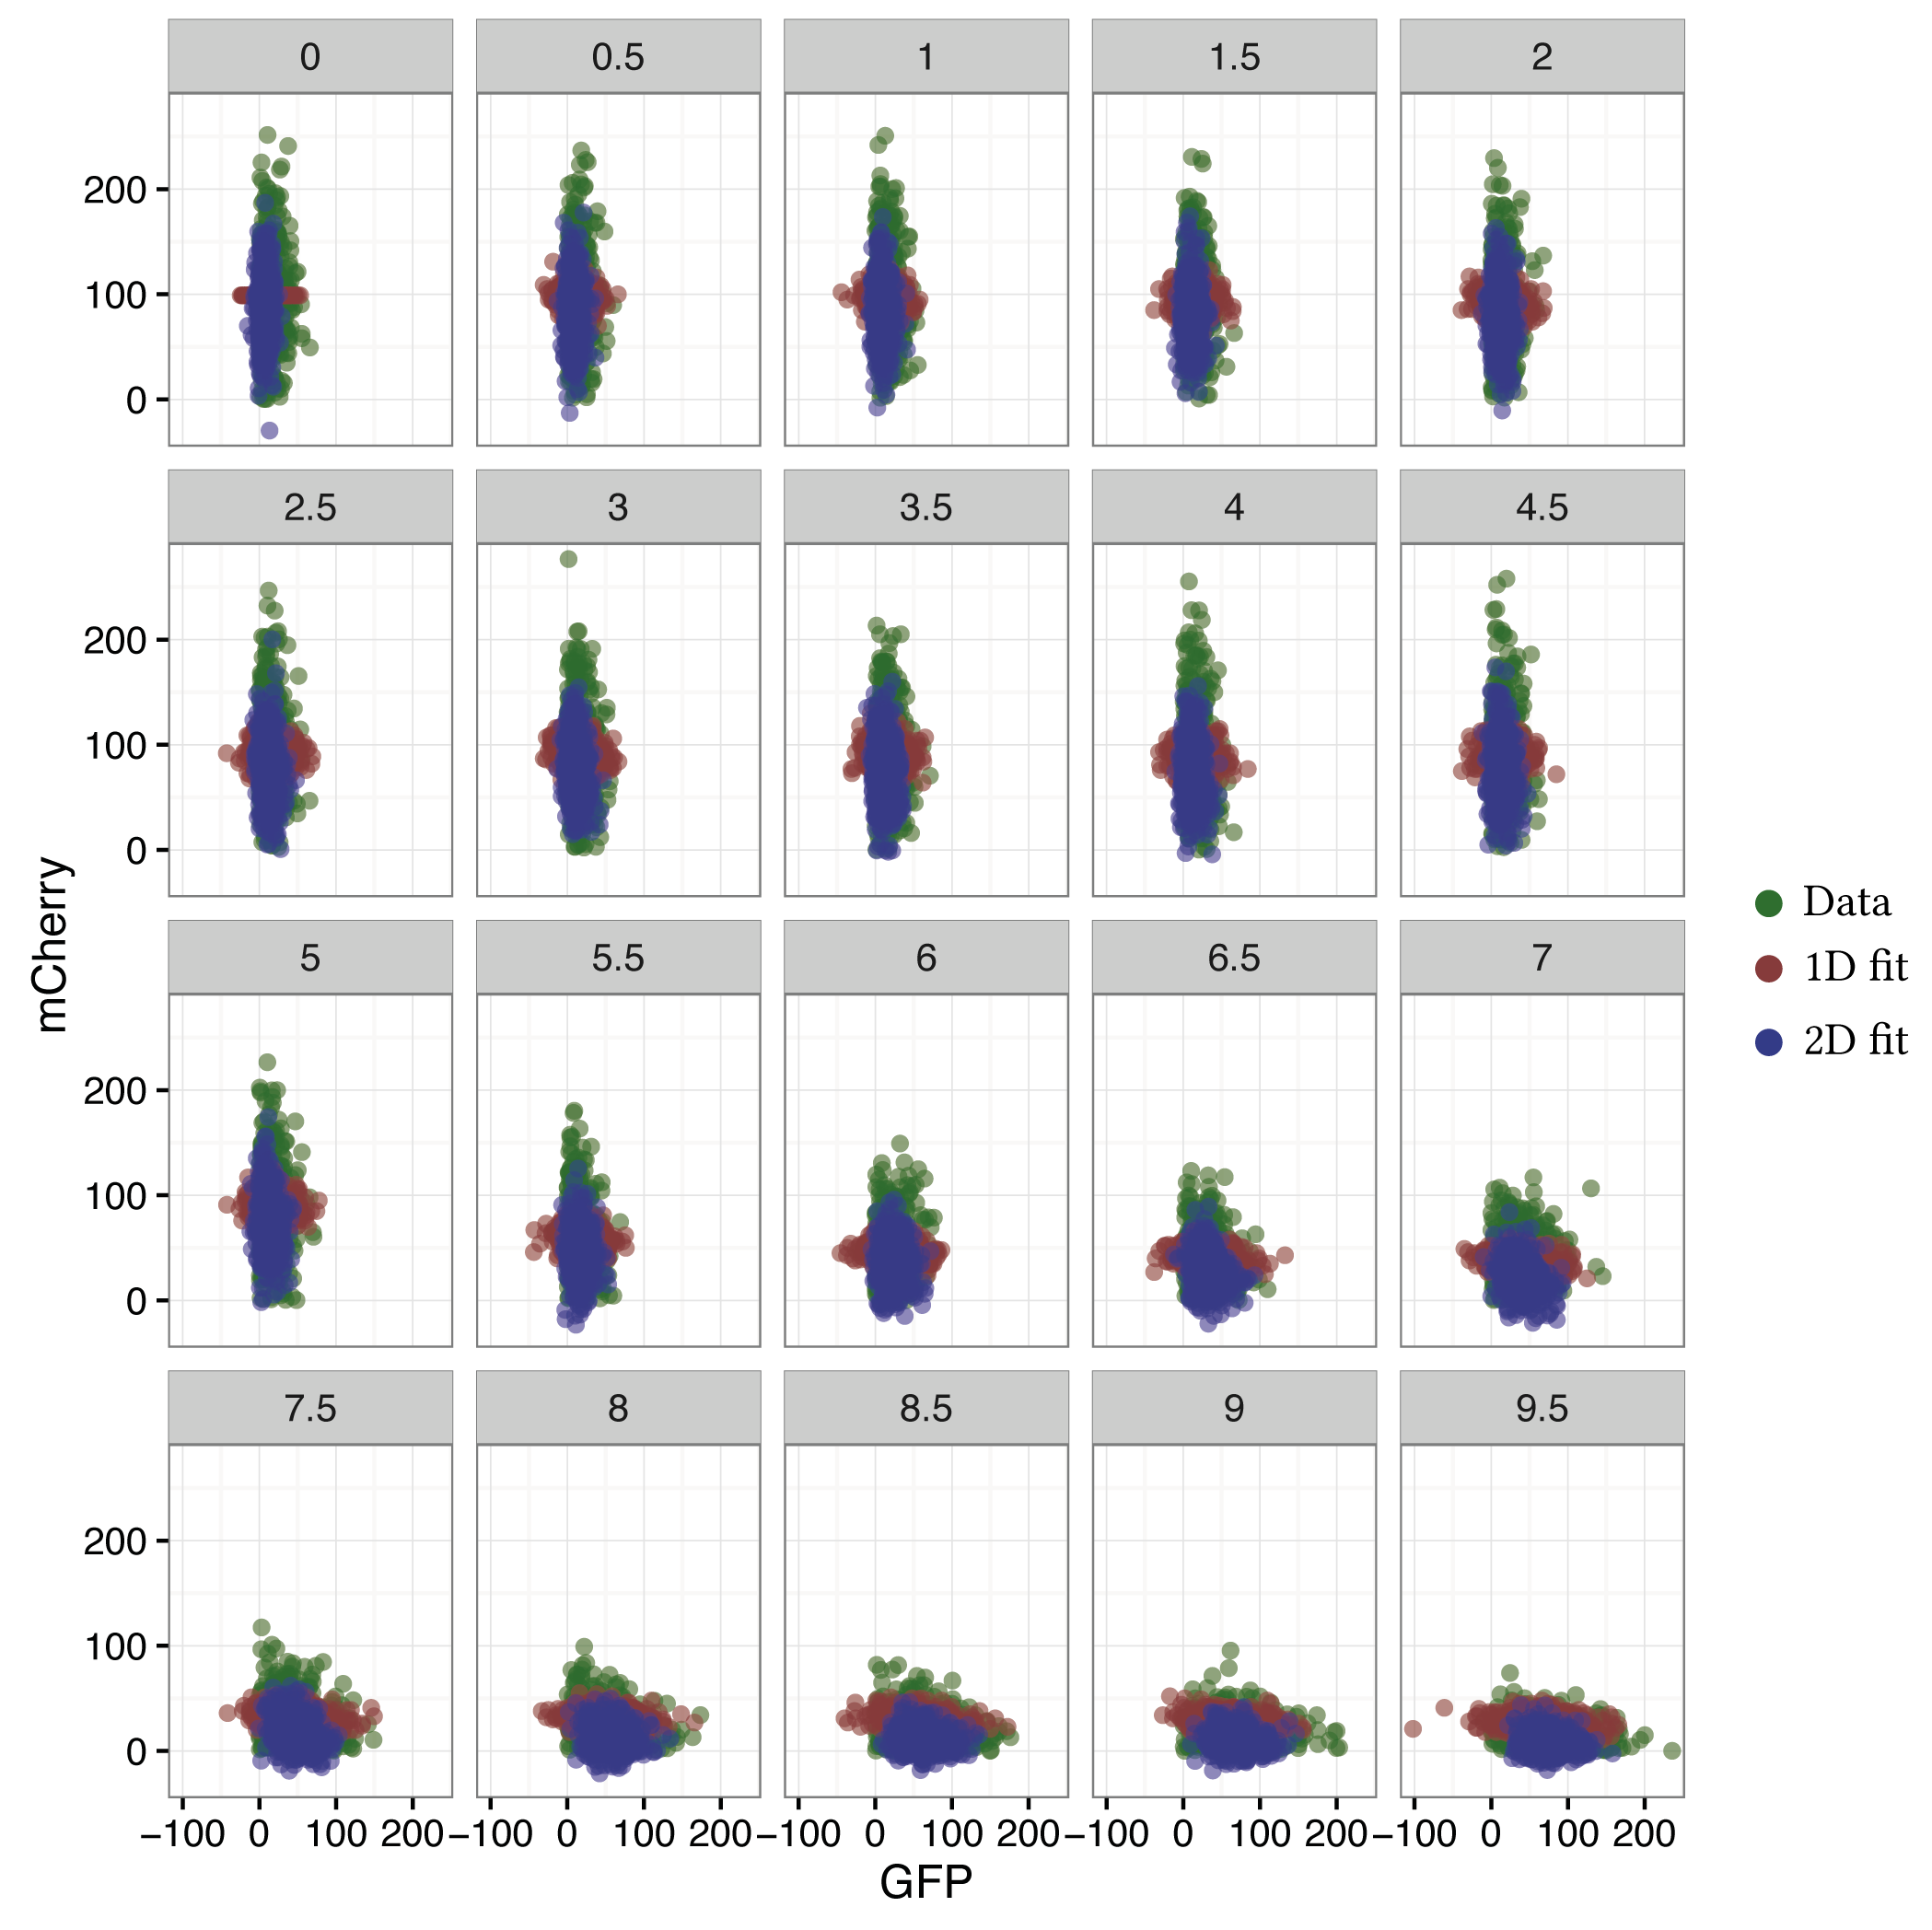
\includegraphics[scale=0.8]{../../chapters/chapterABCFlow/images/1d2dfit.png}
%\caption[LoF caption]{\label{fig:1d2dcomp}Comparing the fits obtained by using the 1D or 2D data. }
%\end{figure}
%\clearpage


 

\begin{figure}[htbp]
\centering
	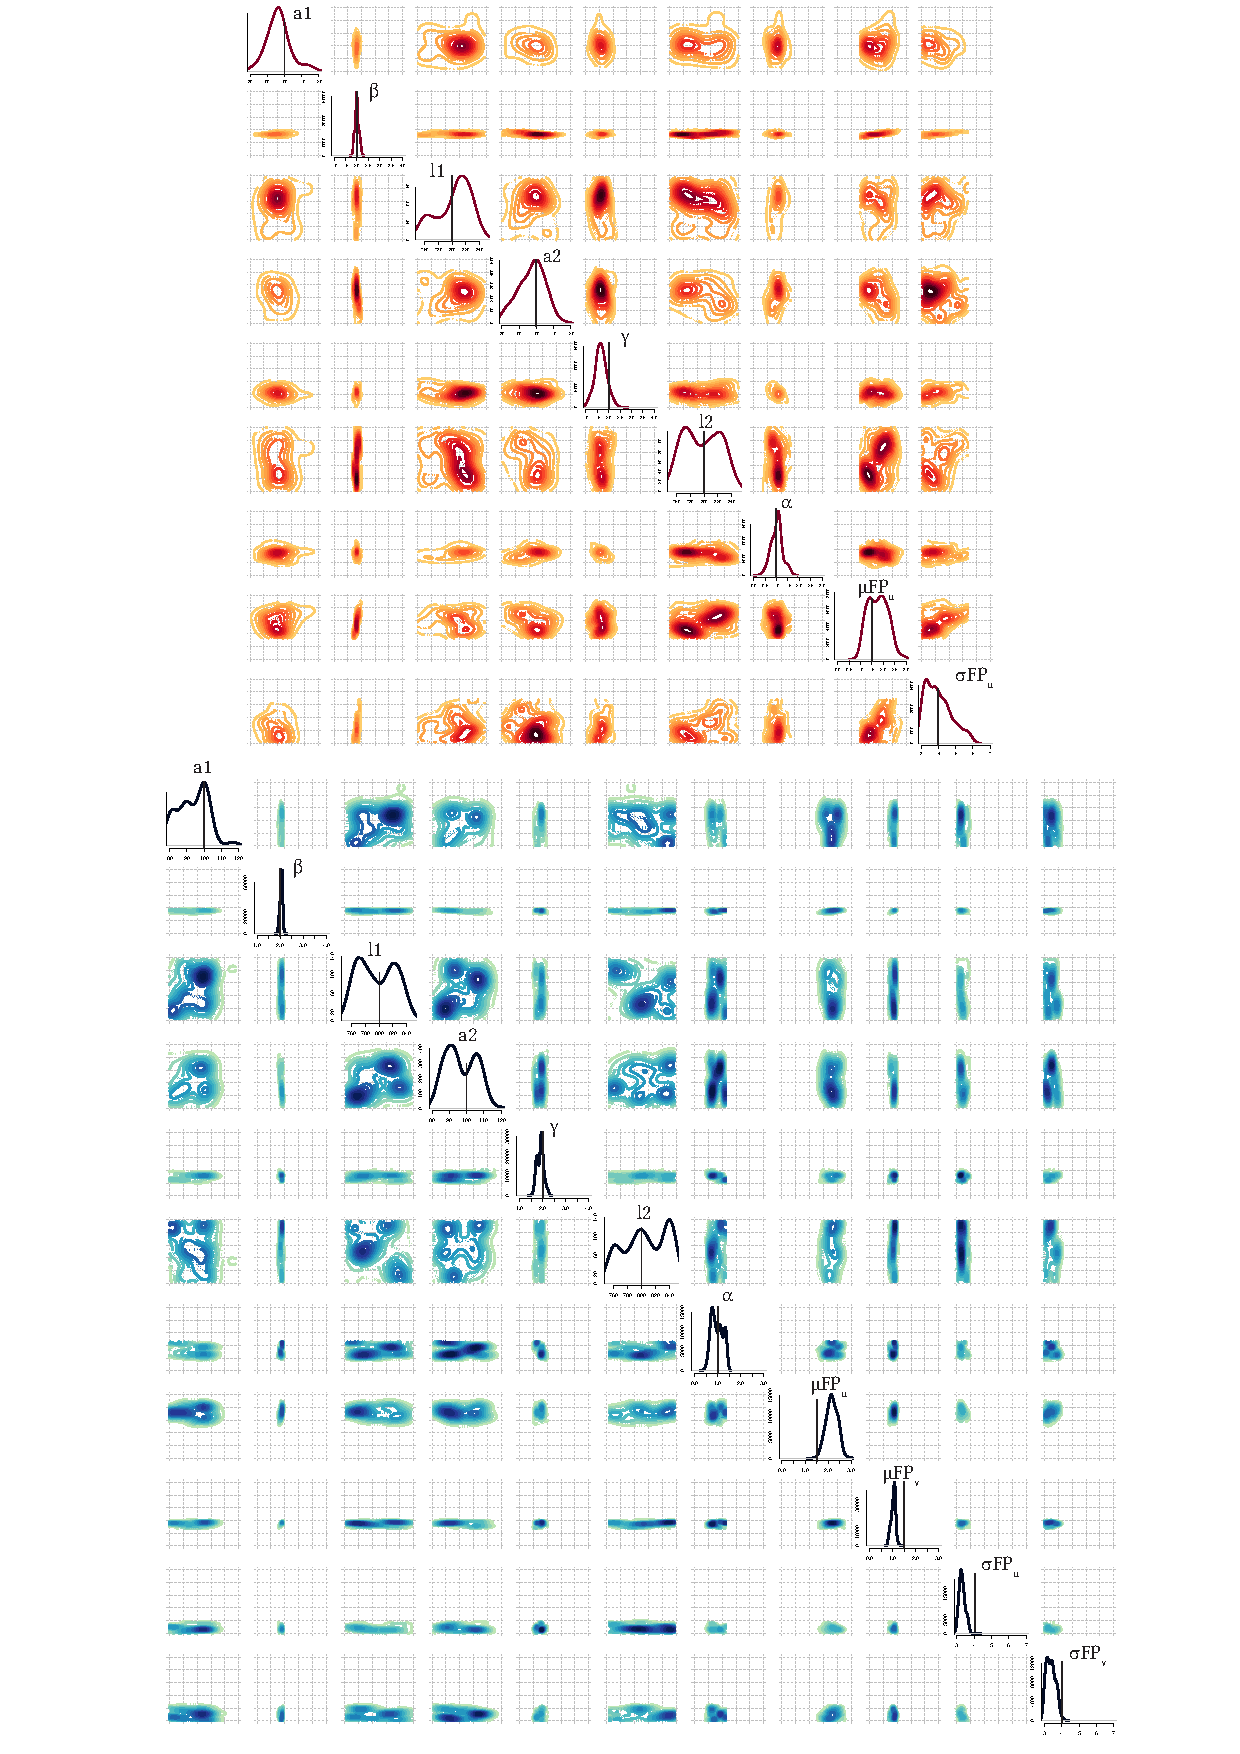
\includegraphics[scale=0.7]{../../chapters/chapterABCFlow/images/toy_model_posteriors.pdf}
	\caption[Posterior distributions of inferred parameters from 1D and 2D simulated data]{\label{fig:1d2d-sim-post} Posterior distributions of inferred parameters from (A) 1D and (B) 2D simulated data. The parameters used to produce the simulated data set were well inferred in both cases. The parameter values used to produce the data are marked on the marginal posterior distributions as a black line.}
\end{figure}

%\begin{figure}[htbp]
%\centering
%	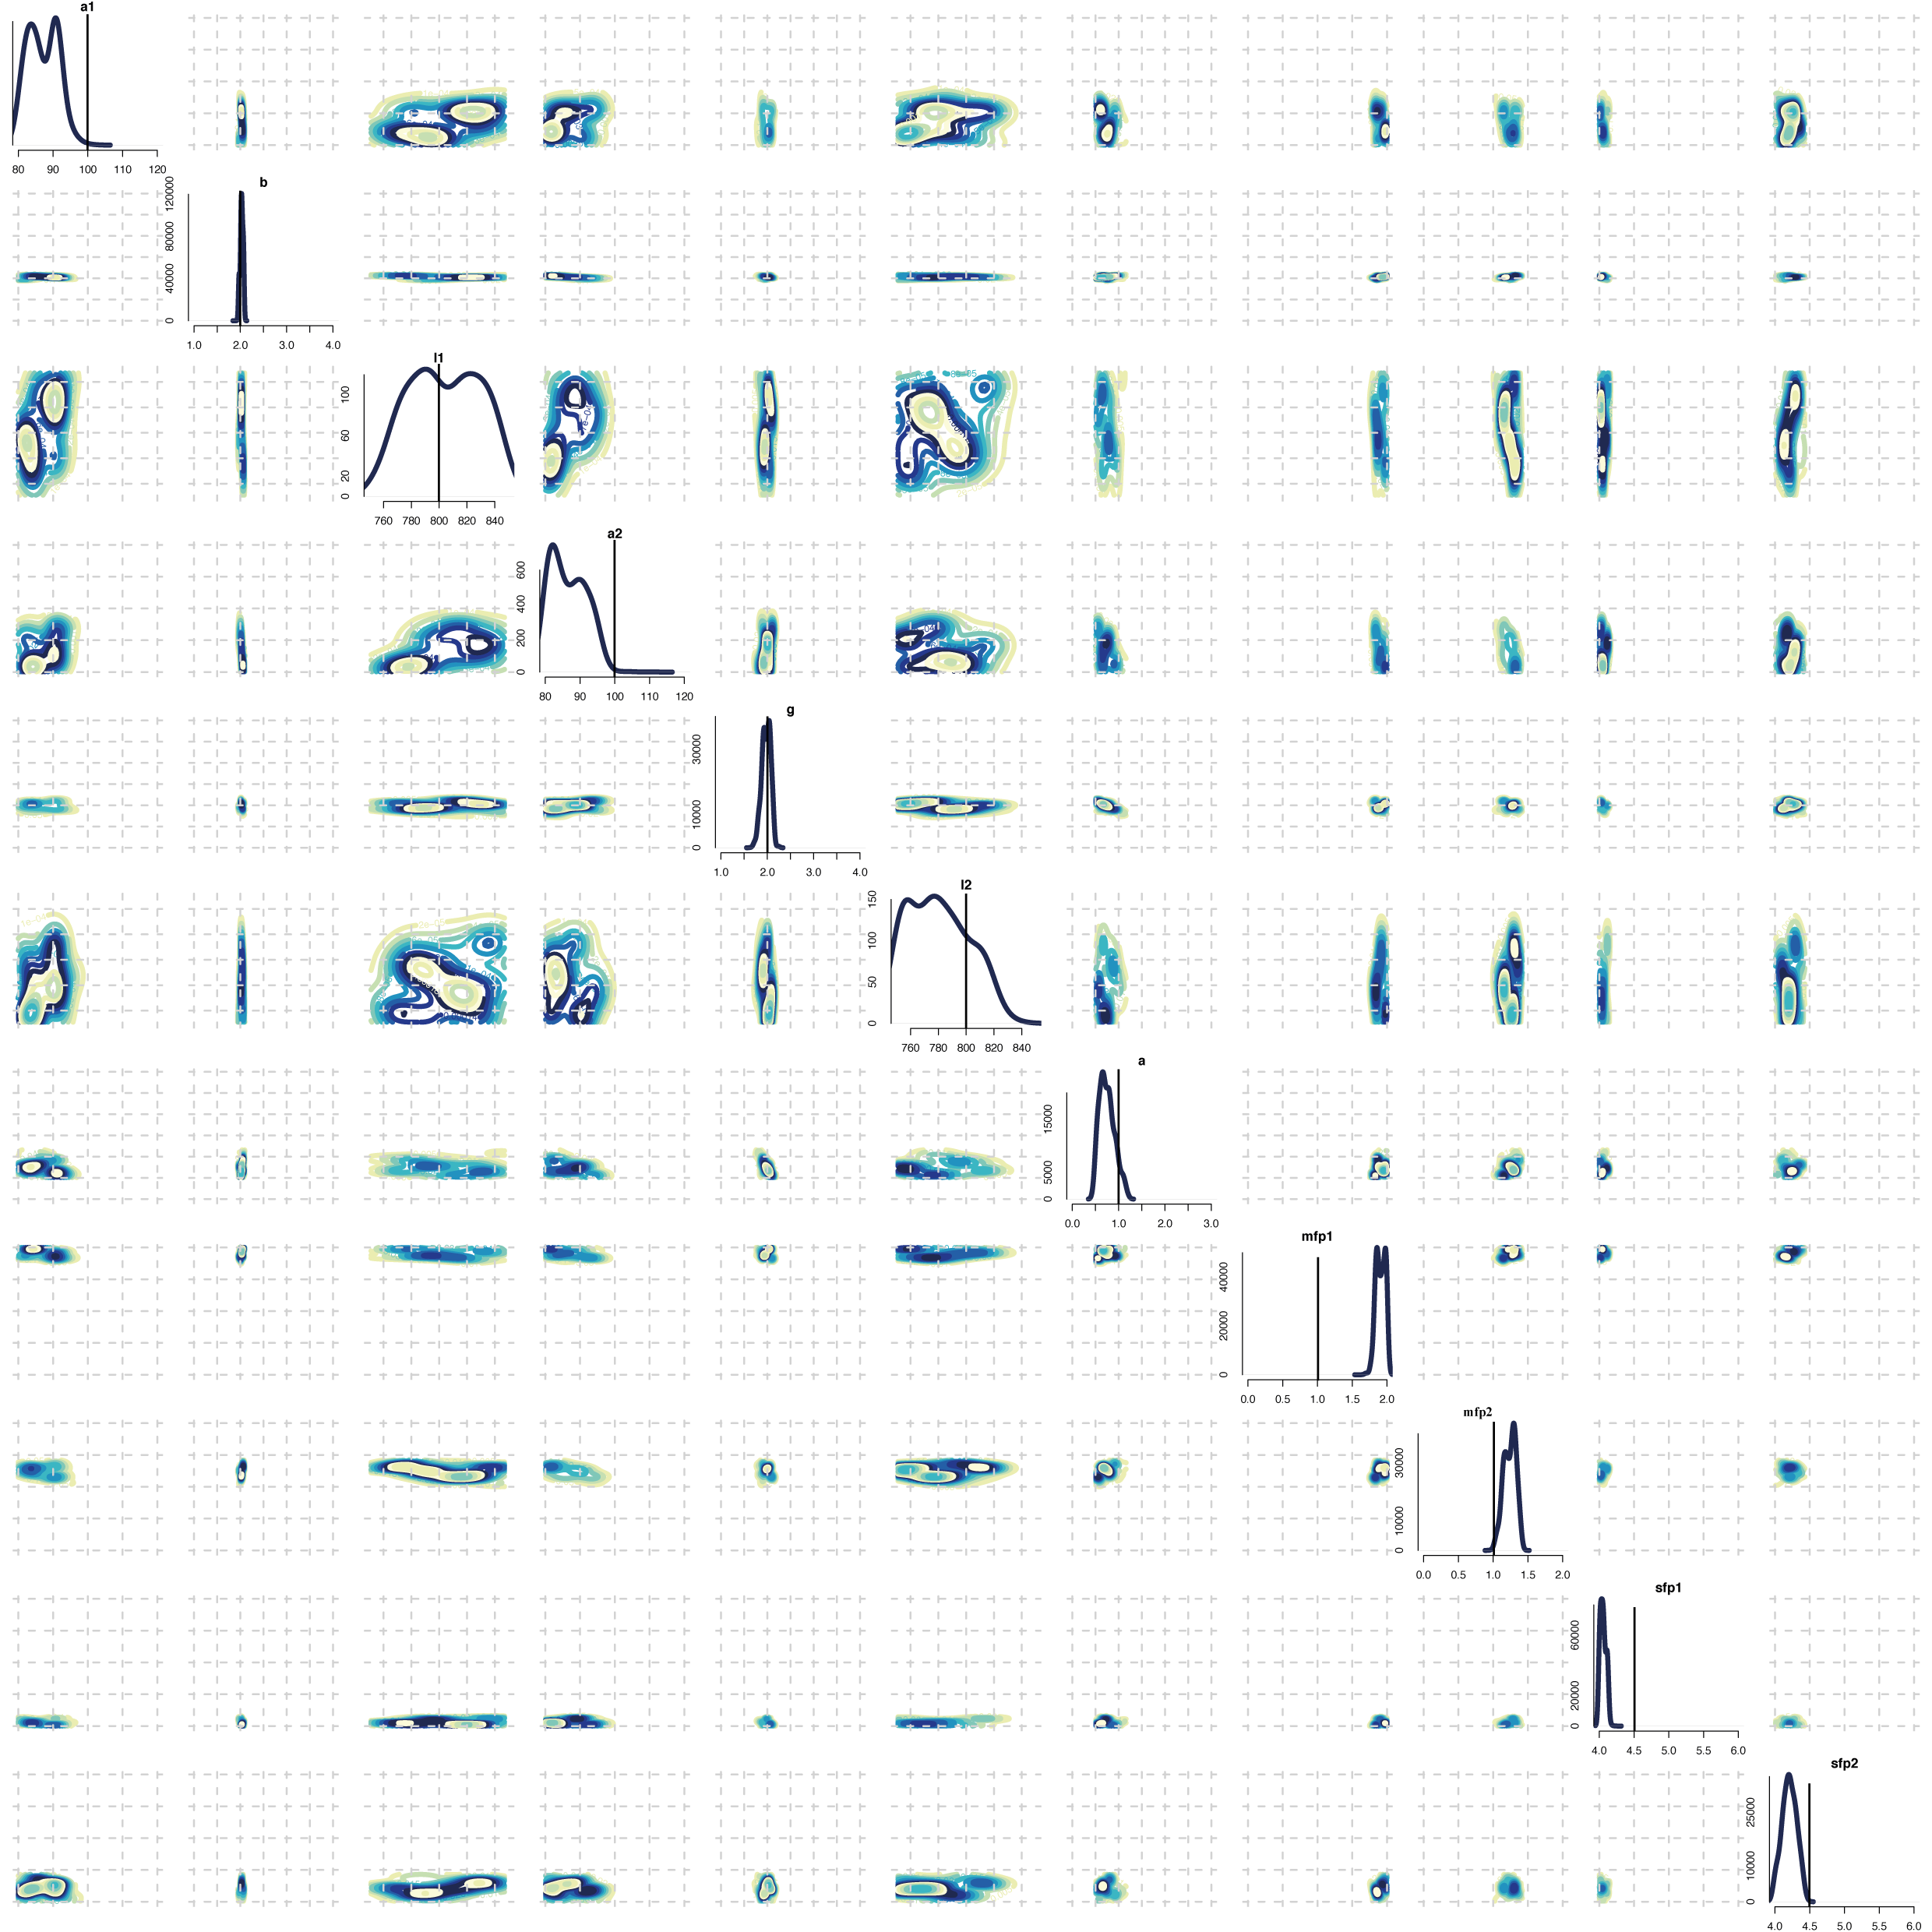
\includegraphics[scale=0.6]{../../chapters/chapterABCFlow/images/toy_model_posterior_2d.png}
%	\caption[Posterior distributions of inferred parameters from the 2D simulated data]{\label{fig:2d-sim-post}The posterior distributions of the 2D fits to simulated data. The parameters used to produce the simulated data set were well inferred in both cases. The parameter values used to produce the data are marked on the marginal posterior distributions as a black line.}
%\end{figure}

%\begin{figure}[htbp]
%\centering%
%	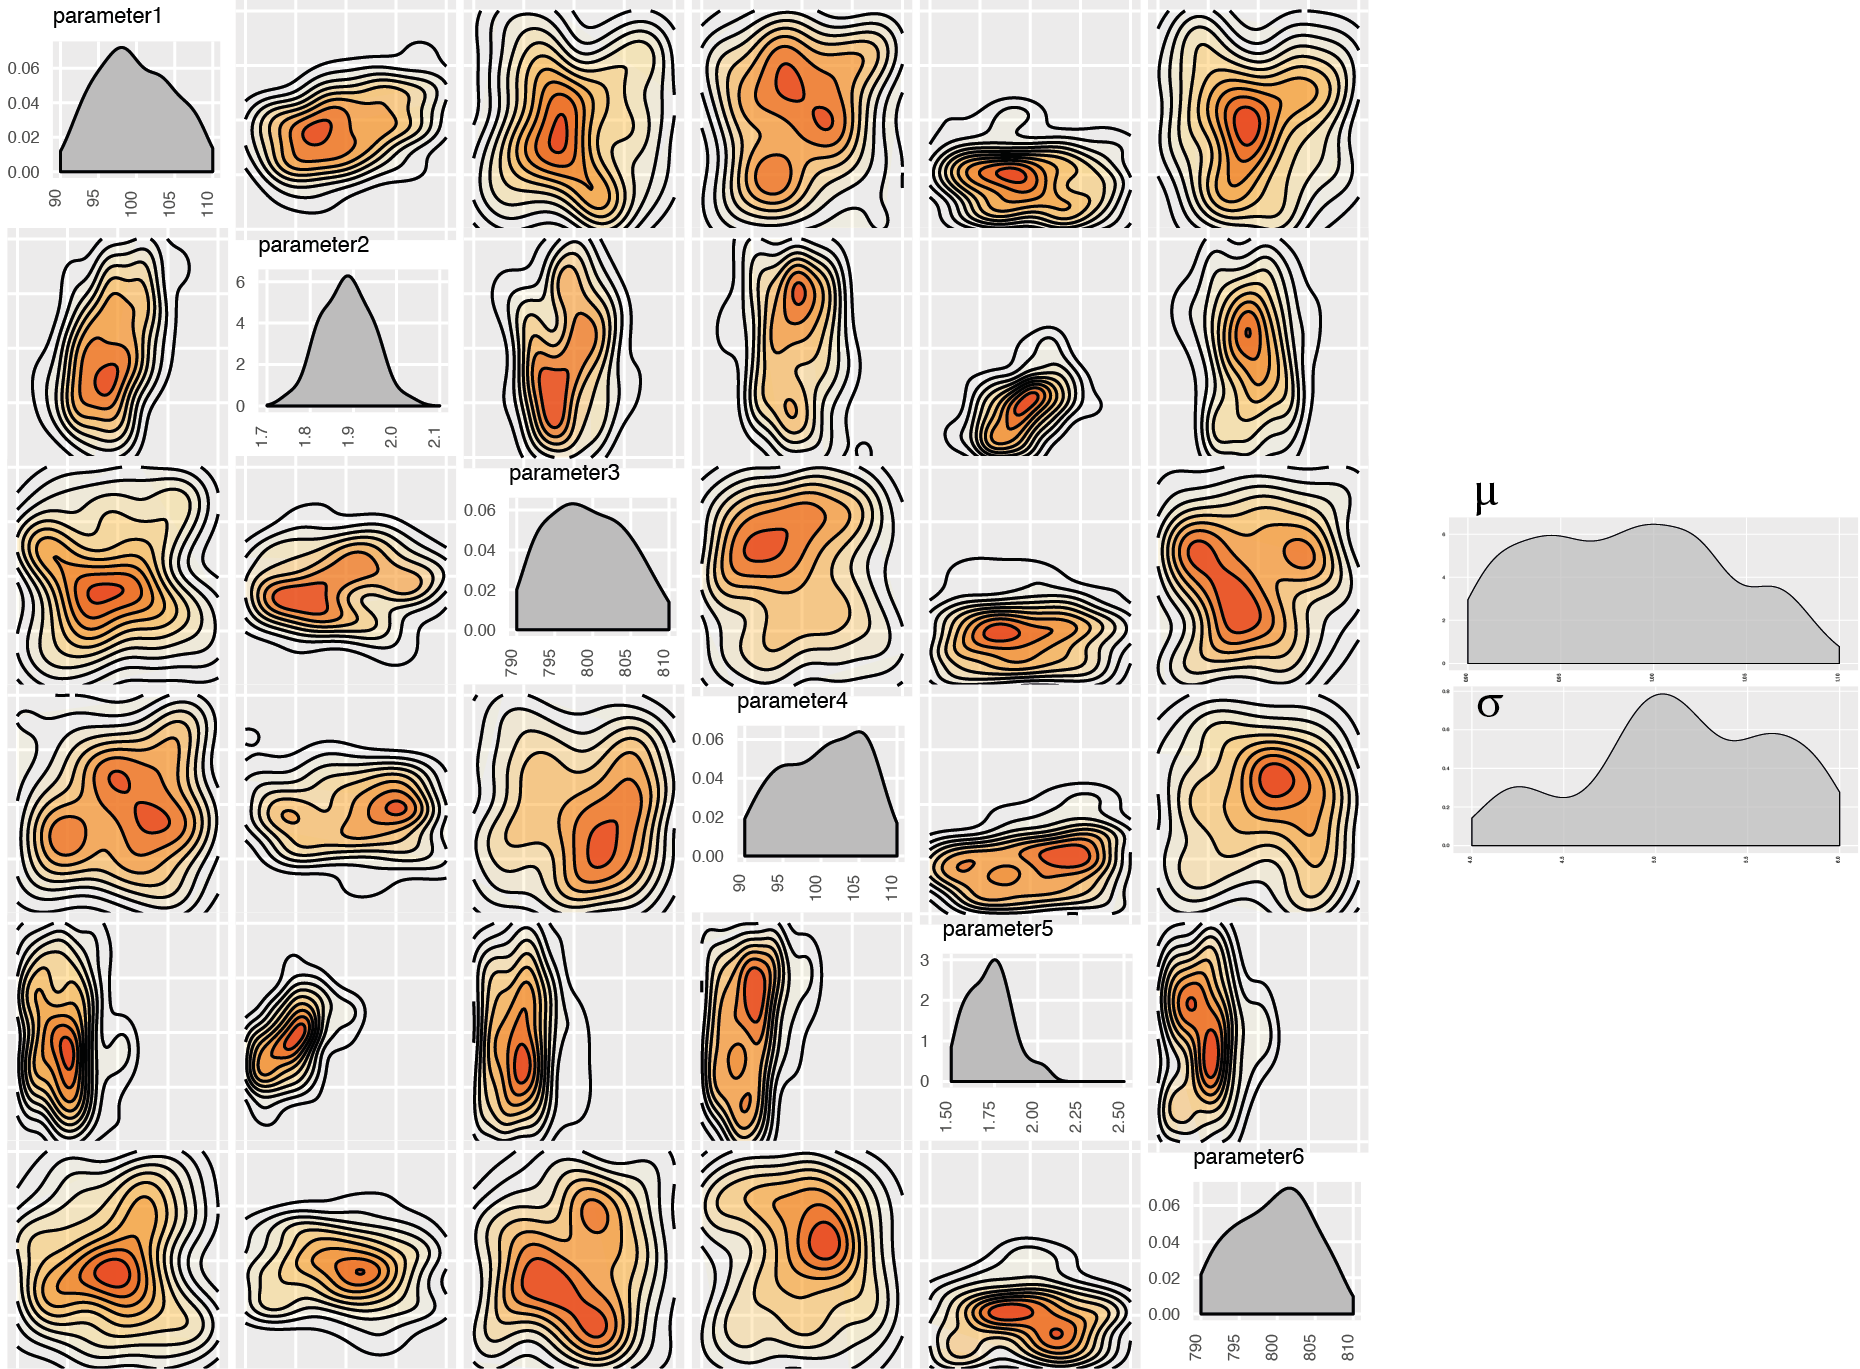
\includegraphics[scale=0.6]{../../chapters/ch	apterABCFlow/images/1d_sim_post.png}%
%	\caption[LoF caption]{\label{fig:1d-sim-post}}
%\end{figure}



%\begin{figure}[htbp]
%\centering
%	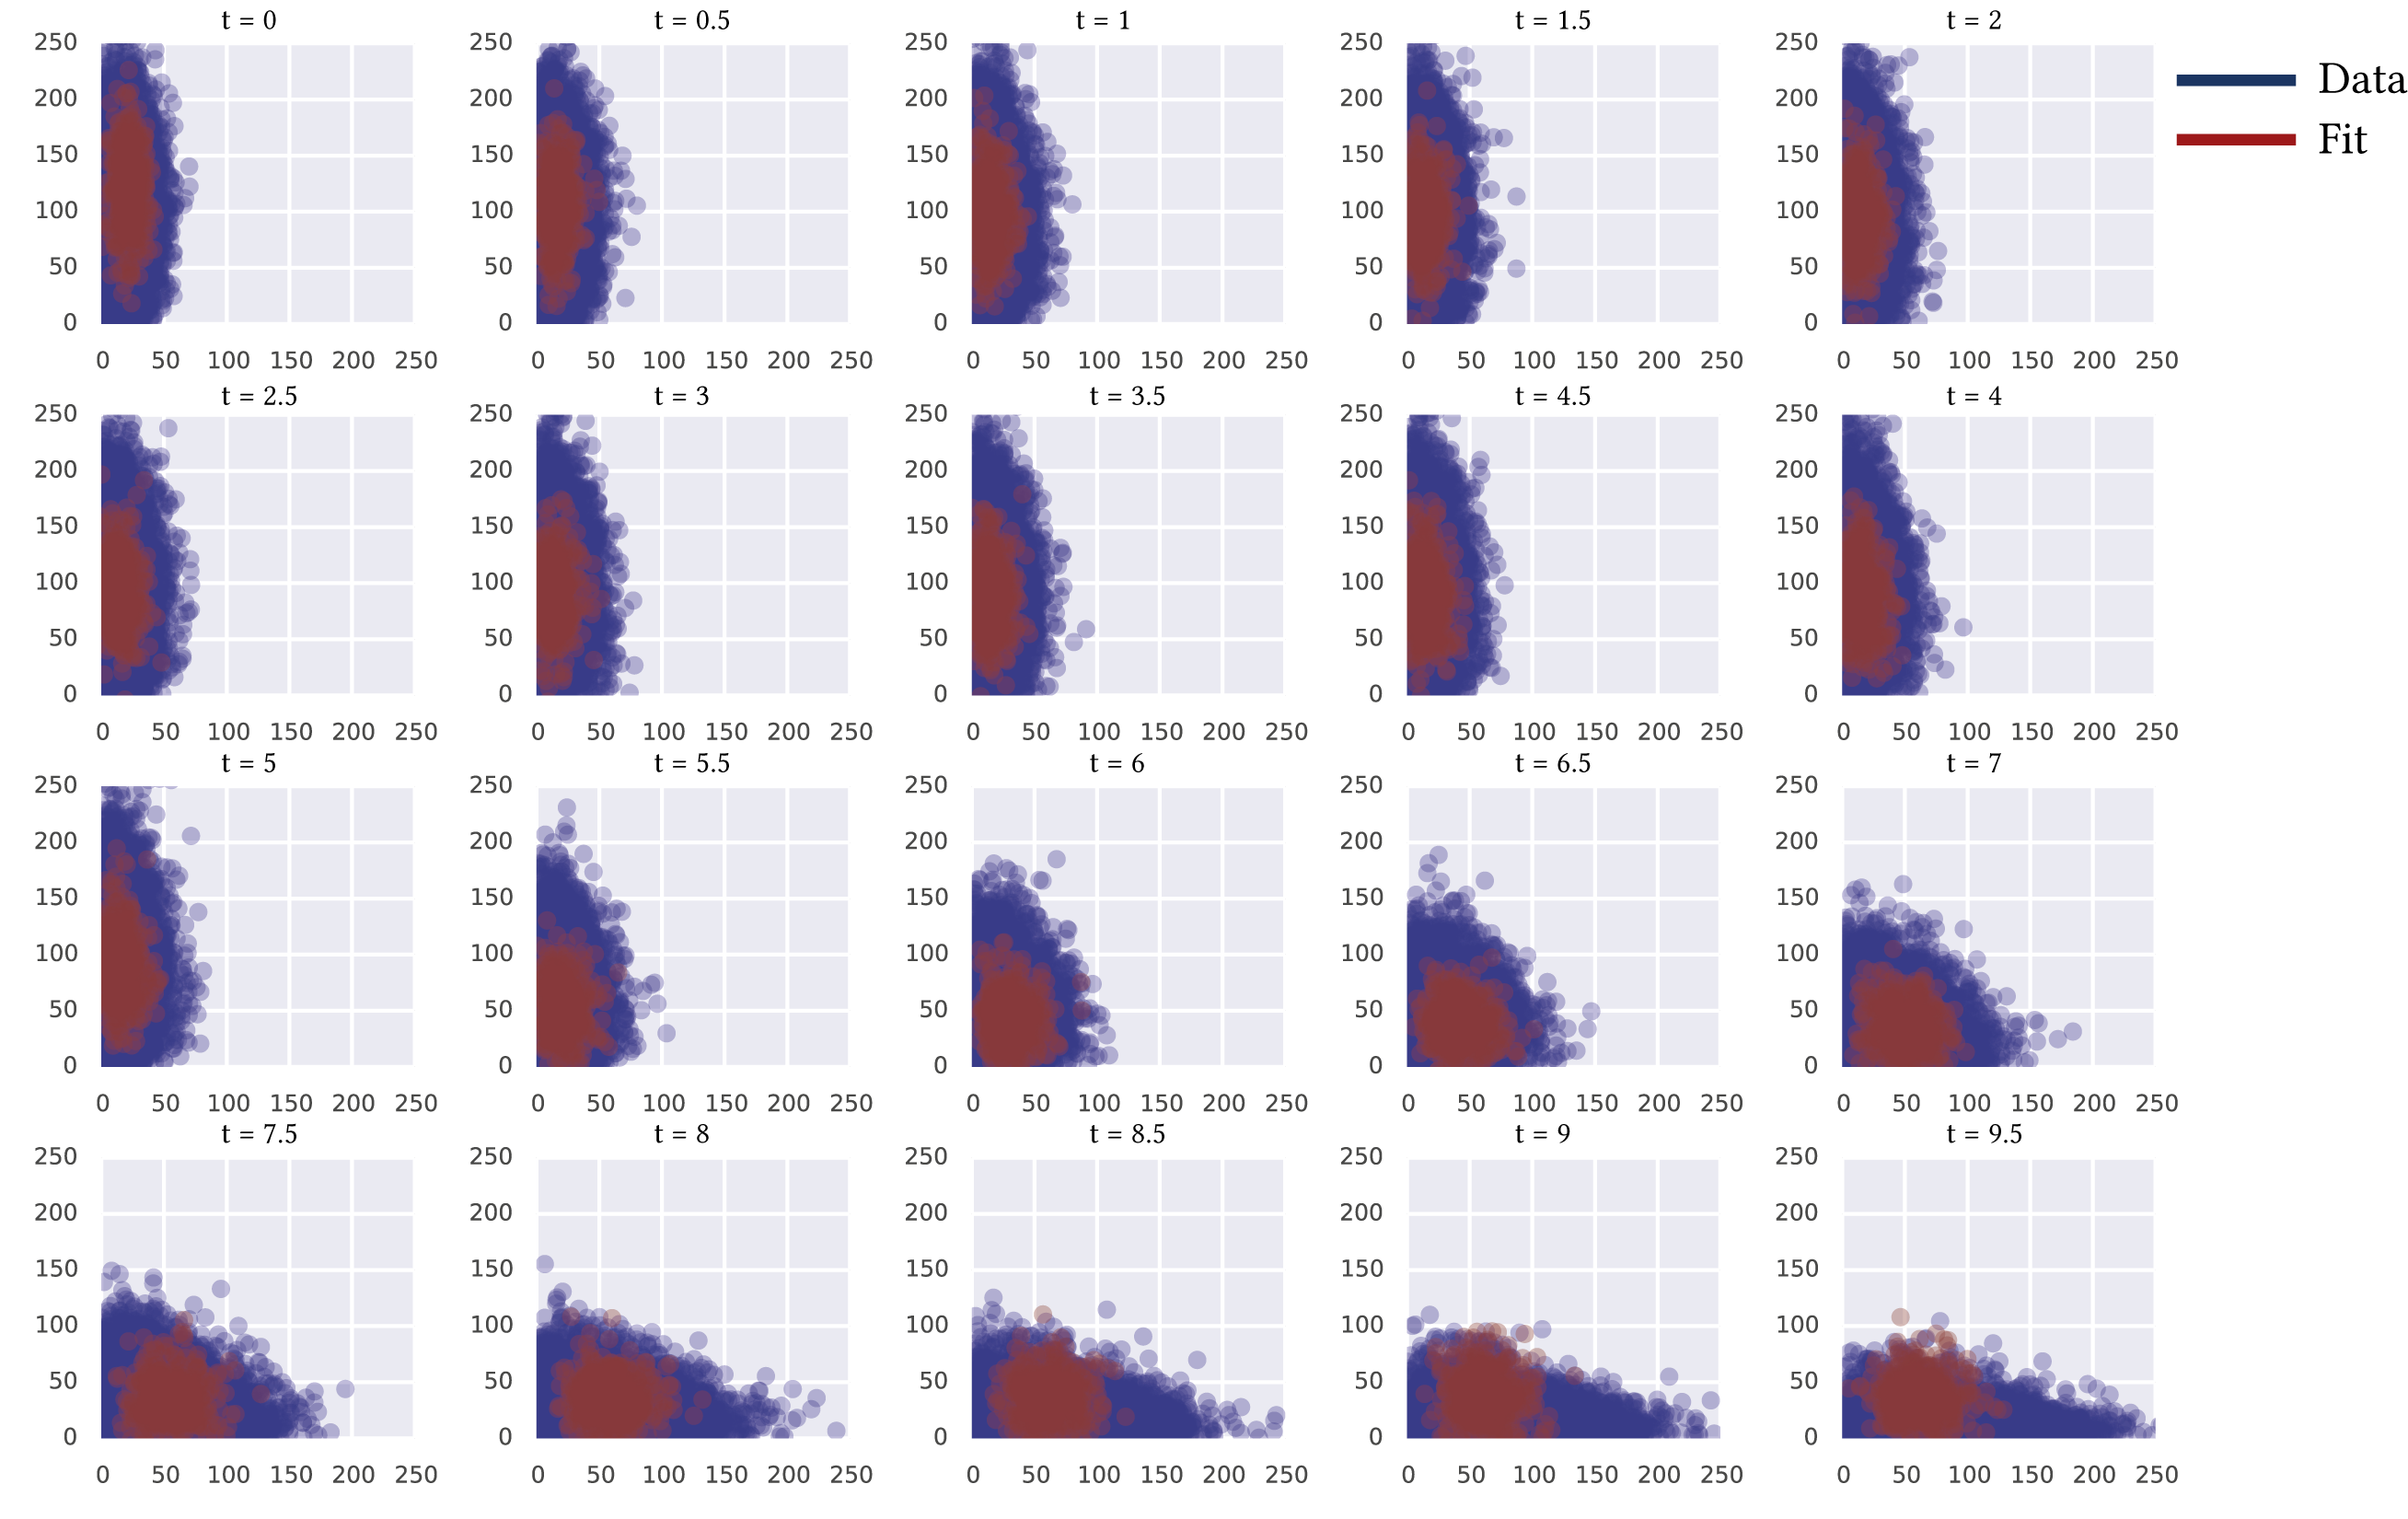
\includegraphics[scale=0.6]{../../chapters/chapterABCFlow/images/2D_sim_res.png}
%	\caption[LoF caption]{\label{fig:2d-sim-res}}
%\end{figure}



\begin{table}[tb]
\centerfloat
\caption{The parameters inferred from simulated data}
\label{tab:inf_params_sim}
\begin{tabular}{ll|lll|lll}
\multirow{3}{*}{Parameters} & \multirow{3}{*}{True value} & \multicolumn{6}{c}{Posterior 95\% credible region} \\ \cline{3-8}
&  & \multicolumn{3}{c|}{1D} & \multicolumn{3}{c}{2D} \\ \cline{3-8} %\cmidrule(l){3-8} 
&  & 0.025 & Median & 0.975 & 0.025 & Median & 0.975 \\ \hline
a\textsubscript{1} & 100 & 83.507 & 96.586 & \multicolumn{1}{l|}{114.485} & 80.064 & 93.539 & 104.940 \\
β & 2 & 1.873 & 2.003 & \multicolumn{1}{l|}{2.167} & 1.926 & 2.063 & 2.131 \\
l\textsubscript{1} & 800 & 755.923 & 807.885 & \multicolumn{1}{l|}{836.913} & 761.972 & 791.912 & 840.872 \\
a\textsubscript{2} & 100 & 80.162 & 98.570 & \multicolumn{1}{l|}{108.148} & 83.362 & 93.726 & 109.974 \\
γ & 2 & 1.195 & 1.642 & \multicolumn{1}{l|}{2.163} & 1.679 & 1.93 & 2.233 \\
l\textsubscript{2} & 800 & 752.757 & 801.021 & \multicolumn{1}{l|}{838.058} & 758.759 & 803.549 & 845.507 \\
α & 1 & 0.495 & 1.055 & \multicolumn{1}{l|}{1.507} & 0.607 & 0.932 & 1.359 \\
μ fp\textsubscript{u} & 1.5 & 1.126 & 1.749 & \multicolumn{1}{l|}{2.542} & 1.762 & 2.164 & 2.546 \\
μ fp\textsubscript{v} & 1.5 &  &  & \multicolumn{1}{l|}{} & 0.826 & 1.067 & 1.413 \\
σ fp\textsubscript{u} & 4 & 3.086 & 3.786 & \multicolumn{1}{l|}{5.712} & 3.028 & 4.053 & 4.121 \\
σ fp\textsubscript{v} & 4 &  &  & \multicolumn{1}{l|}{} & 4.005 & 4.211 & 4.396 \\ \bottomrule
\end{tabular}
\end{table}
\clearpage
These results demonstrate that ABC-Flow can successfully fit a computational model to flow cytometry data. It can identify the parameter values necessary to produce the observed behaviour. ABC-Flow can now be confidently applied to real flow cytometry data of the genetic toggle switch. This allows the inference of the parameter values of toggle switch model producing the data observed. %In the following Section I outline the methods used to obtain the experimental data necessary and the results obtained.


\section{Toggle switch data collection}

In this section I describe the collection of experimental data on the genetic toggle switch. Using flow cytometry and the necessary inducers to flip the switch I study the dynamics over time as well as over different inducer concentrations. 

\subsection{Circuit overview}

The toggle switch plasmid I used here was provided by ~\textcite{Litcofsky:2012gr}. All the switch components were contained in one plasmid, pKDL071. An overview of the plasmid is shown in Figure~\ref{fig:pKDL071map}A. The circuit consists of two promoters, P\textsubscript{trc2} and P\textsubscript{LtetO-1}~\autocite{Lutz:1997ti}. P\textsubscript{trc2} is a LacI repressible promoter. P\textsubscript{LtetO-1} is also a TetR repressible promoter, as shown in Figure~\ref{fig:pKDL071map}B. mCherry~\autocite{Shaner:2004vy} and \acrshort{gfp}~\autocite{SHIMOMURA:1962va} are fluorescent proteins, under the control of the same promoters as the repressors, and thus reflect the levels of TetR and LacI in the system. The plasmid contains kanamycin antibiotic resistance and is high copy (ColE1 origin of replication).

This system is capable of two states, GFP high/mCherry low and GFP low/mCherry high. When \acrshort{iptg} is added to the system, it represses the repression of TetR and mCherry and thus the cells transition to the mCherry high state. When \acrshort{atc} is added to the system, it represses the repression of LacI and GFP and thus the cells transition to the GFP high state. If no inducer is added to the system it will randomly go to the GFP high or mCherry high states.

\begin{figure*}[tb]
	\begin{center}
		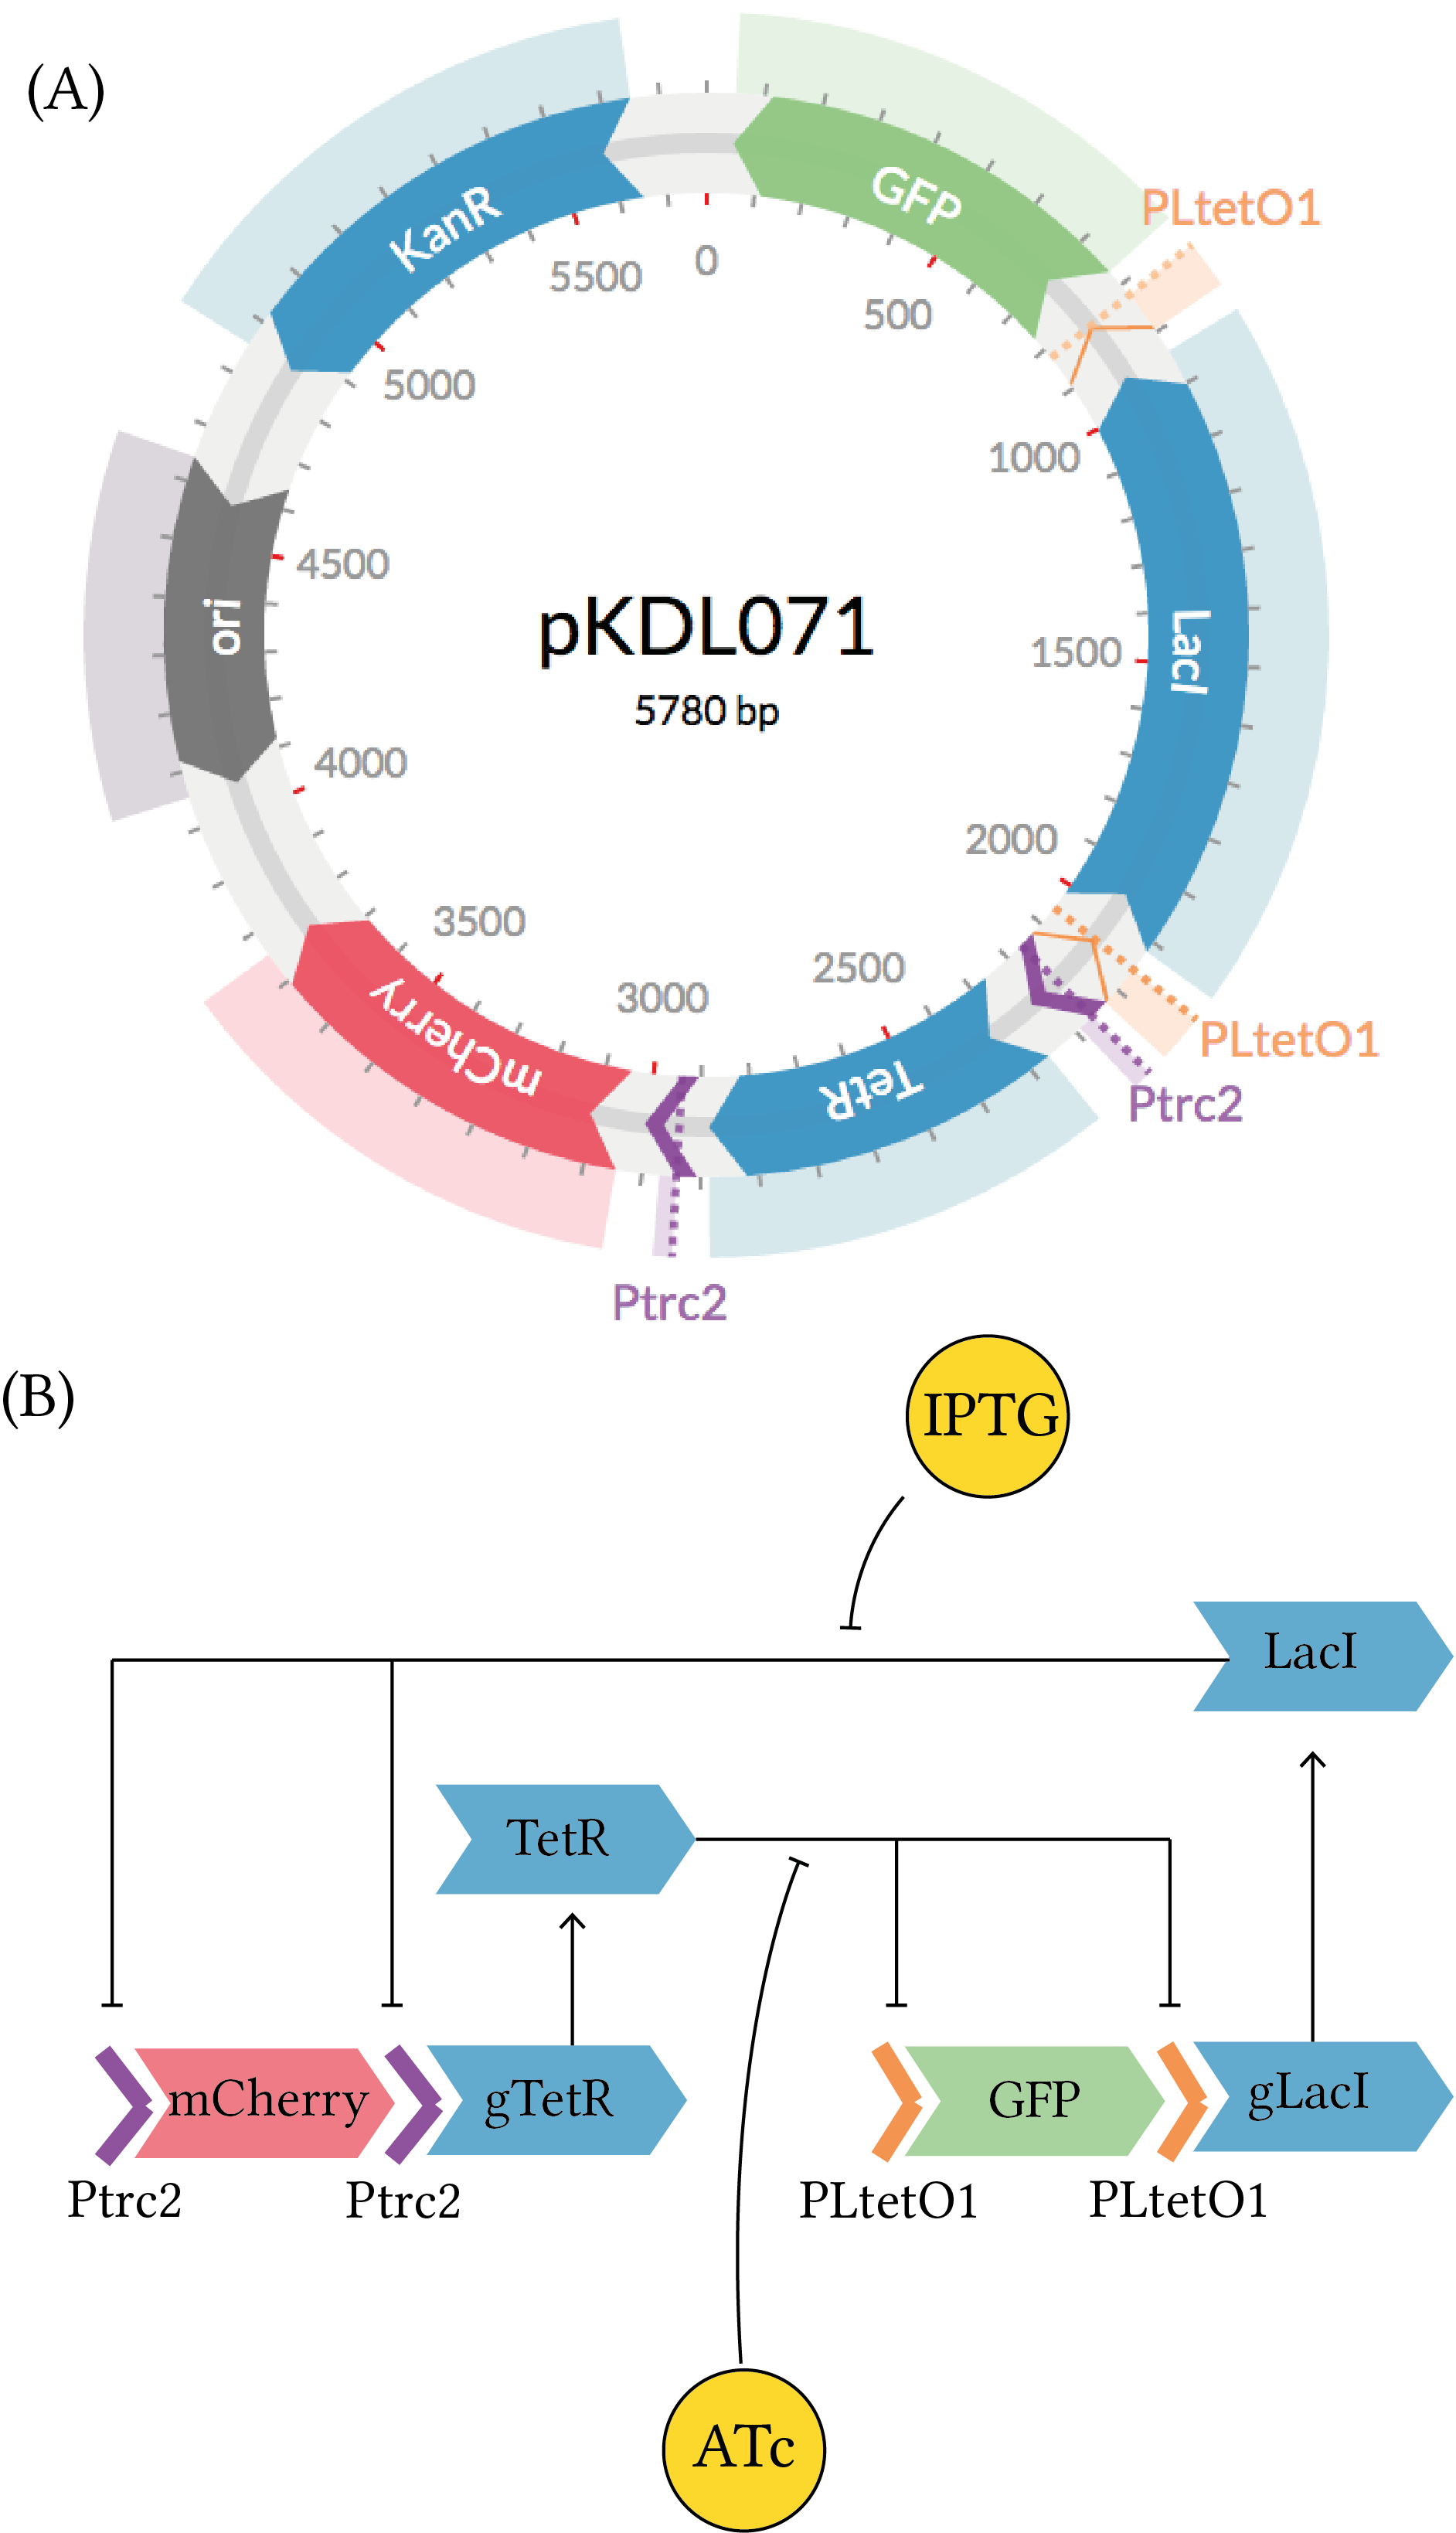
\includegraphics[scale=0.55]{../../chapters/chapterABCFlow/images/pKDL071_overview.png}
	\caption[pKDL071 plasmid map and diagram of interactions]{\label{fig:pKDL071map}The genetic toggle switch circuit used in this chapter. (A) The plasmid map of pKDL071, the plasmid containing the genetic toggle switch used in~\textcite{Litcofsky:2012gr} (B) The interactions between each element of the circuit.}
	\end{center}
\end{figure*}
\clearpage


\subsection{Methods}
\label{sec:experimental_methods}
The toggle switch plasmid was provided by the James J Collins lab in the form of a stab culture in \textit{E. coli} K-12 MG1655.

\subsubsection{\textit{Escherichia coli} culturing conditions}
\label{sec:overnigh_cult}

\acrfull{lb} was made by diluting \acrshort{lb} in deionized water to a concentration of \SI{25}{\gram\per\liter} and subsequently autoclaved at \SI{121}{\celsius} for 15 minutes. \acrshort{lb} agar plates were made by adding bacteriological agar to the above solution to a concentration of \SI{45}{\milli\gram\per\milli\liter} before autoclaving. The solution was then cooled down to \SI{55}{\celsius} using a water bath. If antibiotic was required it was added to the correct concentration to the cooled solution. The solution was then aliquoted to petri dishes and left to solidify at room temperature. The plates were stored in the fridge for up to 1 month. 


Overnight cultures were made by picking a single colony from a static culture on an agar plate. Each colony was placed in \SI{15}{\milli\liter} Falcon tubes (Fisher Scientific, MA, U.S.A) with \SI{5}{\milli\liter} \acrshort{lb} with kanamycin antibiotic at a concentration of \SI{50}{\micro\gram\per\milli\liter}. The tubes were then screwed loosely and taped securely in order to allow for aeration. The falcon tubes were put in an incubator at \SI{37}{\celsius} with orbital shaking at \SI{200} rpm for 12-16 hours. 

\subsubsection{Glycerol stock preparation}
\label{sec:glycerol_stock}
To preserve the transformed cultures long-term glycerol stocks were made. \SI{5}{\milli\liter} \acrshort{lb} and Kanamycin overnight cultures were made as described in Section~\ref{sec:overnigh_cult}. The cultures were kept on ice and \SI{70}\% glycerol was added to the cultures in a ratio of glycerol to culture of 1:7. These were aliquoted into cryovials and transferred to a \SI{-80}{\celsius} freezer for long-term storage.


\subsubsection{Revival}
For subsequent revival of the frozen cultures, a \SI{1.5}{\milli\liter} eppendorf tube was removed from the \SI{-80}{\celsius} freezer and put on ice. A small amount was streaked onto an agar plate containing \acrshort{lb} and kanamycin. The plates were stored in an incubator at \SI{37}{\celsius} overnight. Then the plates were sealed using parafilm and stored at \SI{4}{\celsius} for up to two weeks. 



\subsubsection{Plasmid construction}

Plasmids were constructed via \acrshort{pcr} cloning. \acrshort{pcr} primers were chosen to add restriction enzyme sites on the 5' and 3' where needed. Following \acrshort{pcr} amplification, the amplified \acrshort{dna} was purified using the Qiagen PCR cleanup kit (Qiagen, Crawley, U.K). Double digests were carried out and the desired fragment isolated via gel extraction. The relevant fragments were subsequently ligated. Following construction, each plasmid was isolated using the QIAprep Spin Miniprep Kit (Qiagen, Crawley, U.K). Plasmid concentration was determined using the Thermo Scientific NanoDrop 1000 Spectrophotometer (Fisher Scientific, MA, U.S.A).

\subsubsection{Polymerase Chain Reaction}
\label{sec:pcr}
In order to amplify DNA and add the restriction enzyme sites required, a \acrfull{pcr} reaction was carried out with mutagenic primers. A list of primers can be found in Appendix~\ref{ap:Prim}. Q5\textsuperscript{\textregistered} DNA Polymerase (NEB, MA, U.S.A) was used with its associated buffer, \acrshort{dntp} and Q5\textsuperscript{\textregistered} enhancer, as specified in Table~\ref{tab:pcr_rec}. \acrshort{pcr} reactions were run in a T100\textsuperscript{TM} thermal cycler (Bio-Rad Laboratories, Inc., UK) as per the Q5\textsuperscript{\textregistered} recommendations, and as outlined in Tables~\ref{tab:pcr_rec} and ~\ref{tab:pcr_sched}.

\begin{table}[H]
\centering
\caption{\acrshort{pcr} recipe}
\label{tab:pcr_rec}
\begin{tabular}{@{}ccc@{}}
\toprule
Reagent           & Final concentration & \SI{50}{\micro\liter} reaction \\ \midrule
Q5\textsuperscript{\textregistered} buffer 5X      & 1X                  & \SI{10}{\micro\liter}          \\
\acrshort{dntp}             & \SI{200}{\milli\molar} each          & \SI{1}{\micro\liter}           \\
Forward primer    & \SI{0.5}{\micro\molar}               & \SI{2.5}{\micro\liter}         \\
Reverse primer    & \SI{0.5}{\micro\molar}               & \SI{2.5}{\micro\liter}         \\
Template DNA      & \SI{2}{\micro\gram}/\SI{50}{\micro\liter}                 & -             \\
Q5\textsuperscript{\textregistered} \acrshort{dna} polymerase & \SI{0.02}{\unit\per\micro\liter}            & \SI{0.5}{\micro\liter}         \\
Q5\textsuperscript{\textregistered} enhancer       & 1X                  & \SI{10}{\milli\liter}          \\
\ce{H2O}               & -                   & to \SI{50}{\micro\liter}       \\ \bottomrule
\end{tabular}
\end{table}


\begin{table}[H]
\centering
\caption{Thermocycling conditions}
\label{tab:pcr_sched}
\begin{tabular}{@{}cccc@{}}
\toprule
Step            & Cycles              & Temperature           & Time                 \\ \midrule
Initiation      & 1                   & \SI{98}{\celsius} & \SI{30}{\second} \\
Denaturation    & \multirow{3}{*}{30} & \SI{98}{\celsius} & \SI{10}{\second} \\
Annealing        &                     & \SI{55}{\celsius} -\SI{72}{\celsius} & \SI{20}{\second} \\
Extension       &                     & \SI{72}{\celsius} & \SI{2}{\minute}  \\
Final extension & 1                   & \SI{72}{\celsius} &  30 s/kb  \\
Hold            & 1                   & \SI{4}{\celsius}  & \infty            \\ \bottomrule  
\end{tabular}
\end{table}

\subsubsection{Digestion}
\label{sec:digest}

All enzymes, buffers and \acrfull{bsa} were supplied by NEB. Digestion controls were carried out by adding \ce{H2O} instead of \acrshort{dna} in the digestion reaction. Additionally, during agarose gel electrophoresis uncut plasmid was run alongside the digested plasmid as a further control. 

\SI{1}{\micro\gram} digests were set up by mixing the plasmid with \SI{0.5}{\micro\liter} of each restriction enzyme as per the recipe shown in Table~\ref{tab:digestion}. The reactions were placed in an incubator at \SI{37}{\celsius} for 4 hours. Finally, the solutions were analysed using agarose gel electrophoresis (Section~\ref{sec:gel_electr}).


\begin{table}[htbp]
\centering
\caption{Digestion recipe}
\label{tab:digestion}
\begin{tabular}{@{}cccc@{}}
\toprule
Reagent   & Volume  &  &  \\ \midrule
Pst\RNum{1}&                \SI{0.5}{\micro\liter}     &  &  \\
Hind\RNum{3} &                \SI{0.5}{\micro\liter}     &  &  \\
NEB Buffer 2.1        & \SI{2}{\micro\liter}       &  &  \\
BSA            & \SI{0.2}{\micro\liter}     &  &  \\
\acrshort{dna}              & \SI{1}{\micro\gram}       &  &  \\
\ce{H2O}           & to \SI{20}{\micro\liter} &  &  \\ \bottomrule
\end{tabular}
\end{table}


\subsubsection{Agarose gel electrophoresis}
\label{sec:gel_electr}
To make a 0.8\% agarose gel, \SI{0.4}{\gram} agarose were diluted in \SI{50}{\milli\liter} 1X TAE buffer. It was further dissolved by microwaving for 1-3 minutes. The solution was left to cool for 5 minutes and then \SI{1.5}{\micro\liter} GelRed\textsuperscript{TM} (Biotium, Fremont, CA) was added. Gel trays were prepared by putting the well comb in place and taping the ends shut. The solution wast then poured into the prepared gel trays and left to solidify for 20-30 minutes at room temperature.

Agarose gel electrophoresis was carried out by placing the poured gels into the gel tanks. The tank was then flooded with 1X TAE buffer. The \acrshort{dna} was prepared to be analysed by adding \SI{4}{\micro\liter} loading dye to \SI{20}{\micro\liter} sample. A negative control was used with \ce{H2O} instead of sample. The \acrshort{dna} ladder of choice was prepared by adding \SI{1}{\micro\liter} \ce{H2O} and \SI{1}{\micro\liter} dye to \SI{2}{\micro\liter} ladder. The agarose gel was ran at \SI{90}{\volt} between 45 - 60 minutes.

To purify the fragments from the agarose gel, a sterile razor blade was used to cut out the desired fragment. This was placed in a clean eppendorf tube. The \acrshort{dna} was isolated from the gel using the QIAquick Gel Extraction Kit.

\subsubsection{Ligation}
\label{sec:ligation}
A ratio of 3:1 of insert to recipient plasmid was used, \SI{1}{\micro\liter} T4\textsuperscript{\textregistered}  DNA ligase (NEB, MA, U.S.A) and \SI{2}{\micro\liter} ligase buffer. Molecular biology grade \ce{H2O} was added to make the reaction up to \SI{20}{\micro\liter}. The controls used for each ligation reaction, are shown in Table~\ref{tab:lig-contr}. Control 1 is used to detect competent cell viability, control 2 background due to uncut vector, control 3  re-circularization and control 4 contamination.  

The ligation reactions were placed at \SI{4}{\celsius} for 12 hours. The reactions were then placed at \SI{65}{\celsius} for 10 minutes to heat inactivate the T4 DNA ligase enzyme. A transformation was then carried out as per Section~\ref{sec:transfection}.

\begin{table}[htbp]
\centering
\caption{Ligation controls}
\label{tab:lig-contr}
\begin{tabular}{@{}ccccc@{}}
\toprule
       & Control 1 & Control 2 & Control 3 & Control 4 \\ \midrule
Vector &  Uncut    & \cmark    & \cmark    & \xmark    \\
Insert &  \xmark    & \xmark    & \xmark    & \cmark    \\
Buffer &  \cmark    & \cmark    & \cmark    & \cmark    \\
\ce{H2O}    & \cmark    & \cmark    & \cmark    & \cmark    \\
Ligase &  \xmark    & \xmark    & \cmark    & \cmark    \\ \bottomrule
\end{tabular}
\end{table}


\subsubsection{Transformation}
\label{sec:transfection}
Thermocompetent \textit{E.coli} DH5α was transformed with the constructed plasmids. Each ligation reaction was added to \SI{50}{\micro\liter} of thawed competent cells. The cells were subsequently kept on ice for 30 minutes, then placed at a \SI{42}{\celsius} water bath for \SI{45}{\second}. The cells were then placed back on ice for 15 minutes. Then \SI{500}{\micro\liter} of Super Optimal broth with Catabolite repression (SOC) was added to each ligation and placed in a \SI{37}{\celsius} shaking incubator for 3 hours. \SI{500}{\micro\liter} and \SI{50}{\micro\liter} were subsequently pipetted of each ligation onto petri dishes with LB agar and the appropriate antibiotic. The plates were incubated at \SI{37}{\celsius} for 12-16 hours. Two controls were used for the transfection protocol, a positive control with no antibiotic in the LB agar and non-transfected cells and a negative control of non-transformed cells and LB agar with antibiotic. These ensure that the cells are viable and not contaminated respectively. 

Individual colonies were then selected from each transfection and grew each separately in \SI{5}{\milli\liter} LB medium for 12-16 hours at \SI{37}{\celsius}, 200 rpm. Glycerol stocks were then prepared from each culture, as per Section~\ref{sec:glycerol_stock}.



\subsubsection{Colony \acrshort{pcr}}

In order to determine if the fragment was successfully inserted into the vector \acrshort{dna} plasmid, diagnostic colony \acrshort{pcr} was then carried out. Primers were designed that amplified the multiple cloning site of the vector \acrshort{dna} plasmid. These can be found in Appendix~\ref{ap:Prim}. A \acrshort{pcr} master mix was made for the number of colonies to be amplified, 32, with an added 10\% to account for pipetting error. GoTaq\textsuperscript{\textregistered} Flexi \acrshort{dna} polymerase (Promega Corp., WI, U.S.A.) was used with its associated buffer, \acrshort{dntp} and \ce{MgCl2}and \ce{H2O}. The recipe for the master mix is shown in Table~\ref{tab:pcr_mastex_mix}.

\begin{table}[htbp]
\centering
\caption{Colony \acrshort{pcr} master mix recipe}
\label{tab:pcr_mastex_mix}
\begin{tabular}{@{}ccc@{}}
\toprule
Reagent           & Final concentration & Master mix \\ \midrule
GoTaq\textsuperscript{\textregistered} green Flexi buffer      & 1X                  & \SI{141}{\micro\liter}          \\
\acrshort{dntp}             & \SI{200}{\milli\molar} each          & \SI{14.1}{\micro\liter}           \\
Forward primer    & \SI{0.5}{\micro\molar}               & \SI{1.4}{\micro\liter}         \\
Reverse primer    & \SI{0.5}{\micro\molar}               & \SI{1.4}{\micro\liter}         \\
GoTaq\textsuperscript{\textregistered} Flexi polymerase & \SI{0.02}{\unit\per\micro\liter}            & \SI{3.5}{\micro\liter}         \\
\ce{MgCl2}       & 1X                  & \SI{42.2}{\micro\liter}          \\
\ce{H2O}               &     -               & \SI{465}{\micro\liter}       \\ \bottomrule
\end{tabular}
\end{table}

\SI{19}{\micro\liter} were then added from the master mix to each \acrshort{pcr} tube. Each of the colonies was then lifted from the transformation from the agar plate using a \SI{20}{\micro\liter} pipette tip and added it to a \acrshort{pcr} mix by mixing. The pipette tip was subsequently used to make a scratch into a clean agar plate, and labelled. A \acrshort{pcr} was then carried out according to GoTaq\textsuperscript{\textregistered} Flexi polymerase recommendations, and as shown in Table~\ref{tab:pcr_sched_col}.

\begin{table}[H]
\centering
\caption{Thermocycling conditions for colony \acrshort{pcr}}
\label{tab:pcr_sched_col}
\begin{tabular}{@{}cccc@{}}
\toprule
Step            & Cycles              & Temperature           & Time                 \\ \midrule
Cell lysis      & 1                   & \SI{95}{\celsius} & \SI{10} minutes \\

Denaturation    & \multirow{3}{*}{35} & \SI{95}{\celsius} & \SI{30}{\second} \\
Annealing        &                     & \SI{55}{\celsius} -\SI{72}{\celsius}  & \SI{1} minute \\
Extension       &                     & \SI{72}{\celsius} &  30 s/kb  \\

Final extension & 1                   & \SI{72}{\celsius} & \SI{5}{\minute}  \\
Hold            & 1                   & \SI{4}{\celsius}  & \infty            \\ \bottomrule  
\end{tabular}
\end{table}

Finally a diagnostic agarose gel electrophoresis was carried out as outlined in Section~\ref{sec:gel_electr}.

\subsubsection{Sequencing}
In order to confirm plasmid identity, all plasmids were sequenced using Source Bioscience, Cambridge UK. \SI{10}{\micro\liter}  of each plasmid DNA were submitted at a minimum of \SI{100}{\nano\gram\per\micro\liter} as per the requirements. Primer sequences were also submitted and manufactured by Source Bioscience. Primers can be found in Appendix~\ref{ap:Prim}. 

\subsubsection{Inducers}

Anhydrotetracycline (aTc) solution was made by diluting \acrshort{atc} from Cayman Chemical Company in \SI{100}\% ethanol to a concentration of \SI{1}{\milli\gram\per\milli\liter}. \acrfull{iptg} solution was made by dissolving \acrshort{iptg} in deionized water to a concentration of \SI{1}{\molar}. The solution was sterilised by passing the solution through a \SI{0.22}{\micro\meter} syringe filter. Both inducers were stored in \SI{1}{\milli\liter} aliquots at \SI{-20}{\celsius}. 


\subsubsection{Growth rate measurement}
\label{sec:growth_meth}
Plate reader analysis was carried out in order to measure the growth of \textit{E.coli} over time. Overnight cultures were made using the method shown in Section~\ref{sec:overnigh_cult}. Overnight cultures were then diluted by a 1:1000 ratio into a \SI{5}{\milli\liter} \acrshort{lb} + kanamycin solution. The diluted cultures were grown at \SI{37}{\celsius} with shaking at 200rpm for 1 hour. These cultures were then further diluted by a 1:100 ratio. \SI{200}{\ul} aliquots of the dilutions were then transferred to a clear flat bottom, black-walled 96-well plate. Wells with only LB and kanamycin were also added in order to be used as blanks. The plate was then sealed using a gas permeable membrane and placed in a BMG FLUOstat OPTIMA plate reader to measure absorbance. The plate reader was set to a constant \SI{37}{\celsius}, with 30 seconds orbital shaking at \SI{150}rpm and \SI{4}{\milli\metre} shaking width every ten minutes. Absorbance was measured at \SI{540}{\nano\meter}. Data was exported as a CSV file and analysed using Python. 

\subsubsection{Flow cytometry}
Flow cytometry experiments were carried out in order to get fluorescence levels in single cells. Flow cytometry data was exported as FCS files and analysed using the R bioconductor packages flowCore~\autocite{flowCore:man}, flowViz~\autocite{flowViz:man} and Ggplot2~\autocite{ggplot2:bk}. Prior to analysis the raw data was processed to remove any debris or instrument noise detected. The data was also processed to removed any doublets, which occurs when more than one bacterial  cell passes through the detector at a time. This will skew the data by including datapoint with double the fluorescent intensity that the rest of the population. The pre-processing was done by using the side scattering data. The height and the area of the sample forward scattering distribution is recorded during an experiment. The cells that lie in the diagonal where the area equals the height are single bacterial cells. If the area of the signal exceeds the height it is indicative of a doublet, or cluster of cells, and is removed from the data. This pre-processing was carried out using autoGate, developed by~\textcite{Fedorec2016}. 



\subsubsection{Concentration assays}
\label{sec:flo_conc}
Concentration assays were carried out in order to determine the concentration of each inducer (\acrshort{atc} and \acrshort{iptg}) at which the switch flips.  Separate overnight cultures were prepared as per Section~\ref{sec:overnigh_cult} with added \acrshort{iptg} at a concentration of \SI{1}{\milli\molar} or added \acrshort{atc} at a concentration of \SI{100}{\nano\gram\per\milli\liter}~\autocite{Litcofsky:2012gr}. The cultures were then diluted by 1:1000 into fresh \acrshort{lb} medium with varying concentrations of the opposite inducer than what the cells were grown in overnight. The concentrations used are shown in Table~\ref{tab:flow_conc}. For each concentration. three replicates cultures were made.


\begin{table}[tb]
\centering
\caption{Concentrations used for flow cytometry assay}
\label{tab:flow_conc}
\begin{tabular}{@{}cc@{}}
\toprule
\acrshort{atc} (ng/ml)  & \acrshort{iptg} (M) \\ \midrule
0.05 & 1e-7 \\
0.06 & 6e-7 \\
0.07 & 1e-6 \\
0.08 & 6e-6 \\
0.09 & 1e-5 \\
0.1  & 1e-3 \\
1.0  & 0.1  \\ \bottomrule
\end{tabular}
\end{table}

The cultures were placed in an incubator at \SI{37}{\celsius}, 200rpm for 5 hours. The cultures were then placed in a centrifuge and spun at 13,000rpm for 5 minutes. The supernatant was discarded and replaced it with \SI{1}{\milli\liter} PBS solution. The BD LSRFortessa\textsuperscript{TM} cell analyzer (Becton, Dickinson and Company) was used at the St. Mary's Flow Cytometry Core Facility at Imperial College London  for flow cytometry analysis. \acrshort{gfp} was excited using the \SI{488}{\nano\meter} laser and detected using the 533/30 filter. mCherry was excited using the \SI{561}{\nano\meter} laser and detected using the 620/10 filter. Data was obtained at n=10000 events per experiment. 

\subsubsection{Time course assays}
\label{sec:flo_time}
Time course assays were carried out to measure the time it takes for the switch to flip to each state. Separate overnight cultures of pKDL071 were prepared as per Section~\ref{sec:overnigh_cult} with added \acrshort{iptg} at a concentration of \SI{1}{\milli\molar} or added \acrshort{atc} at a concentration of \SI{100}{\nano\gram\per\milli\liter}~\autocite{Litcofsky:2012gr}. Overnight cultures of pSEVA281G and pSEVA281C were also made. The cultures were then diluted by a ratio of 1:1000 into fresh LB medium. Separate cultures for each time point were made, in triplicate. For cultures grown overnight in \acrshort{iptg}, \acrshort{atc} was added at a concentration of \SI{100}{\nano\gram\per\milli\liter} and for cultures grown overnight in \acrshort{atc}, \acrshort{iptg} was added at a concentration of \SI{1}{\milli\molar}. All cultures were placed at \SI{37}{\celsius}, 200rpm incubator. At 30 minutes, 1 hour and then every hour up to 6 hours flow cytometry was carried out for the corresponding cultures. Triplicates for each induction were removed from the incubator and placed in a centrifuge at 13, 000rpm for 10 minutes. The supernatant was discarded and replaced with \SI{1}{\milli\liter} PBS solution. These cultures were then analysed in an Attune\textsuperscript{TM} NxT Flow Cytometer (Thermo Fisher Scientific) at University College London. \acrshort{gfp} was excited using the \SI{488}{\nano\meter} laser and detected using the 533/30 filter. mCherry was excited using the \SI{561}{\nano\meter} laser and detected using the 620/10 filter. Data was obtained at n=10000 events per experiment. pSEVA281G and pSEVA281C cultures were used to set the laser voltages and pKDL071 cultures to detect the bacteria population.  


\subsection{Results}

\subsubsection{pKDL071 plasmid alteration}


The pKDL071 plasmid contains all the elements of the switch. The two states of the switch are LacI high and TetR high. These are detected by using the fluorescent proteins that are controlled by the same promoters, and thus mirror the levels of LacI and TetR. The concentration of LacI can be estimated by GFP intensity and TetR concentration by mCherry intensity. In order to detect GFP and mCherry levels within each cell simultaneously, flow cytometry can be used. The lasers needed to excite GFP and mCherry are \SI{488}{\nano\meter} blue and \SI{561}{\nano\meter} yellow respectively. Since the blue laser was not available for use in the BD Accuri\textsuperscript{TM} C6 or the BD LSRII\textsuperscript{TM} (Becton, Dickinson and Company) flow cytometers available, an alternative construct had to be made in order to be able to detect the levels of both sides of the switch. 

In order to alter the switch construct to be able to detect both sides, the mCherry gene was swapped for the YFP gene. The yellow fluorescent protein is excited by the blue laser and could thus be detected using the equipment available. The YFP gene was available from BioBrick registry of standard biological parts as BBa\_K592101. PCR cloning was used to introduce the flanking sequences of EcoRV and KasI restriction enzymes in the 5' and 3' ends respectively. The primers used are given in Appendix~\ref{ap:Prim} . A double digest was performed on plasmids pKDL071 and BBa\_K592101, as well as positive and negative controls. Following gel extraction and ligation, the pKDL071-YFP plasmid was complete. The plasmid map is shown in Figure~\ref{fig:pkdl071yfp}.

\begin{figure*}[tb]
	\begin{center}
		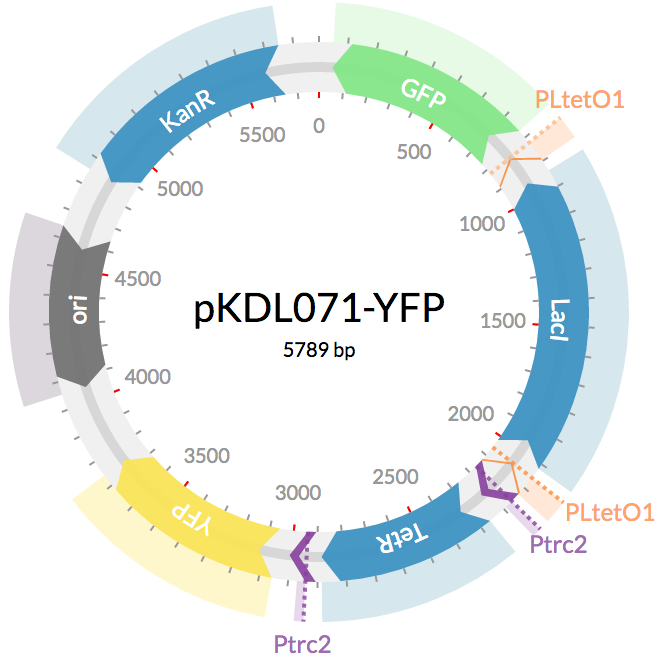
\includegraphics[scale=0.3]{../../chapters/chapterABCFlow/images/pKDL071-YFP.png}
		\caption[pKDL071-YFP plasmid map ]{\label{fig:pkdl071yfp} pKDL071-YFP plasmid map.  }
	\end{center}
\end{figure*}

GFP and YFP have overlapping emission spectra, which have to be compensated during flow cytometry data acquisition~\autocite{Shapiro:1941}. This is because the signal from GFP can be detected at the YFP detector and vice versa. Due to the high level of compensation needed to be carried out and the relatively dim signal given by the bacteria used here, the different stages of the switch, ON and OFF, could not be resolved (data not shown). In order to be able to acquire toggle switch flow cytometry data, an alternative facility was found that was able to detect GFP and mCherry fluorescence. 

\subsubsection{Control plasmids construction}
I constructed two plasmids in order to use them for the flow cytometry mCherry/GFP experiments. The first plasmid, pSEVA281G contains the promoter PLtetO-1 and \acrshort{gfp} and the other, pSEVA281C (supplied by Esteban Martinez García), contains the promoter Ptrc2 and mCherry from PKDL071, shown in Figure~\ref{fig:psevas}. These two plasmids were used to determine the appropriate voltages for the lasers that excite \acrshort{gfp} and mCherry.

pSEVA281G was constructed by digesting pKDL071 and pSEVA281 using the protocol outlined in Section~\ref{sec:digest}. pSEVA281 is a plasmid backbone containing kanamycin resistance, a high copy origin of replication (pUC) and a multiple cloning site. The digested fragments were isolated using gel purification (Section~\ref{sec:gel_electr}) and then ligated the isolated fragments (Section~\ref{sec:ligation}). \textit{Escherichia coli} DH5α was then transformed with each plasmid (Section~\ref{sec:transfection}). 

pSEVA281C was constructed via \acrshort{pcr} cloning. \acrshort{pcr} was carried out using the pKDL071 plasmid as a template \acrshort{dna} using the protocol outlined in Section~\ref{sec:pcr}. Primers were chosen so that Ptrc2 and mCherry were copied and a Hind\RNum{3} restriction enzyme recognition sequence added to the fragment. The rest of the cloning procedure followed as per plasmid pSEVA281G.

\begin{figure*}[tb]
	\begin{center}
		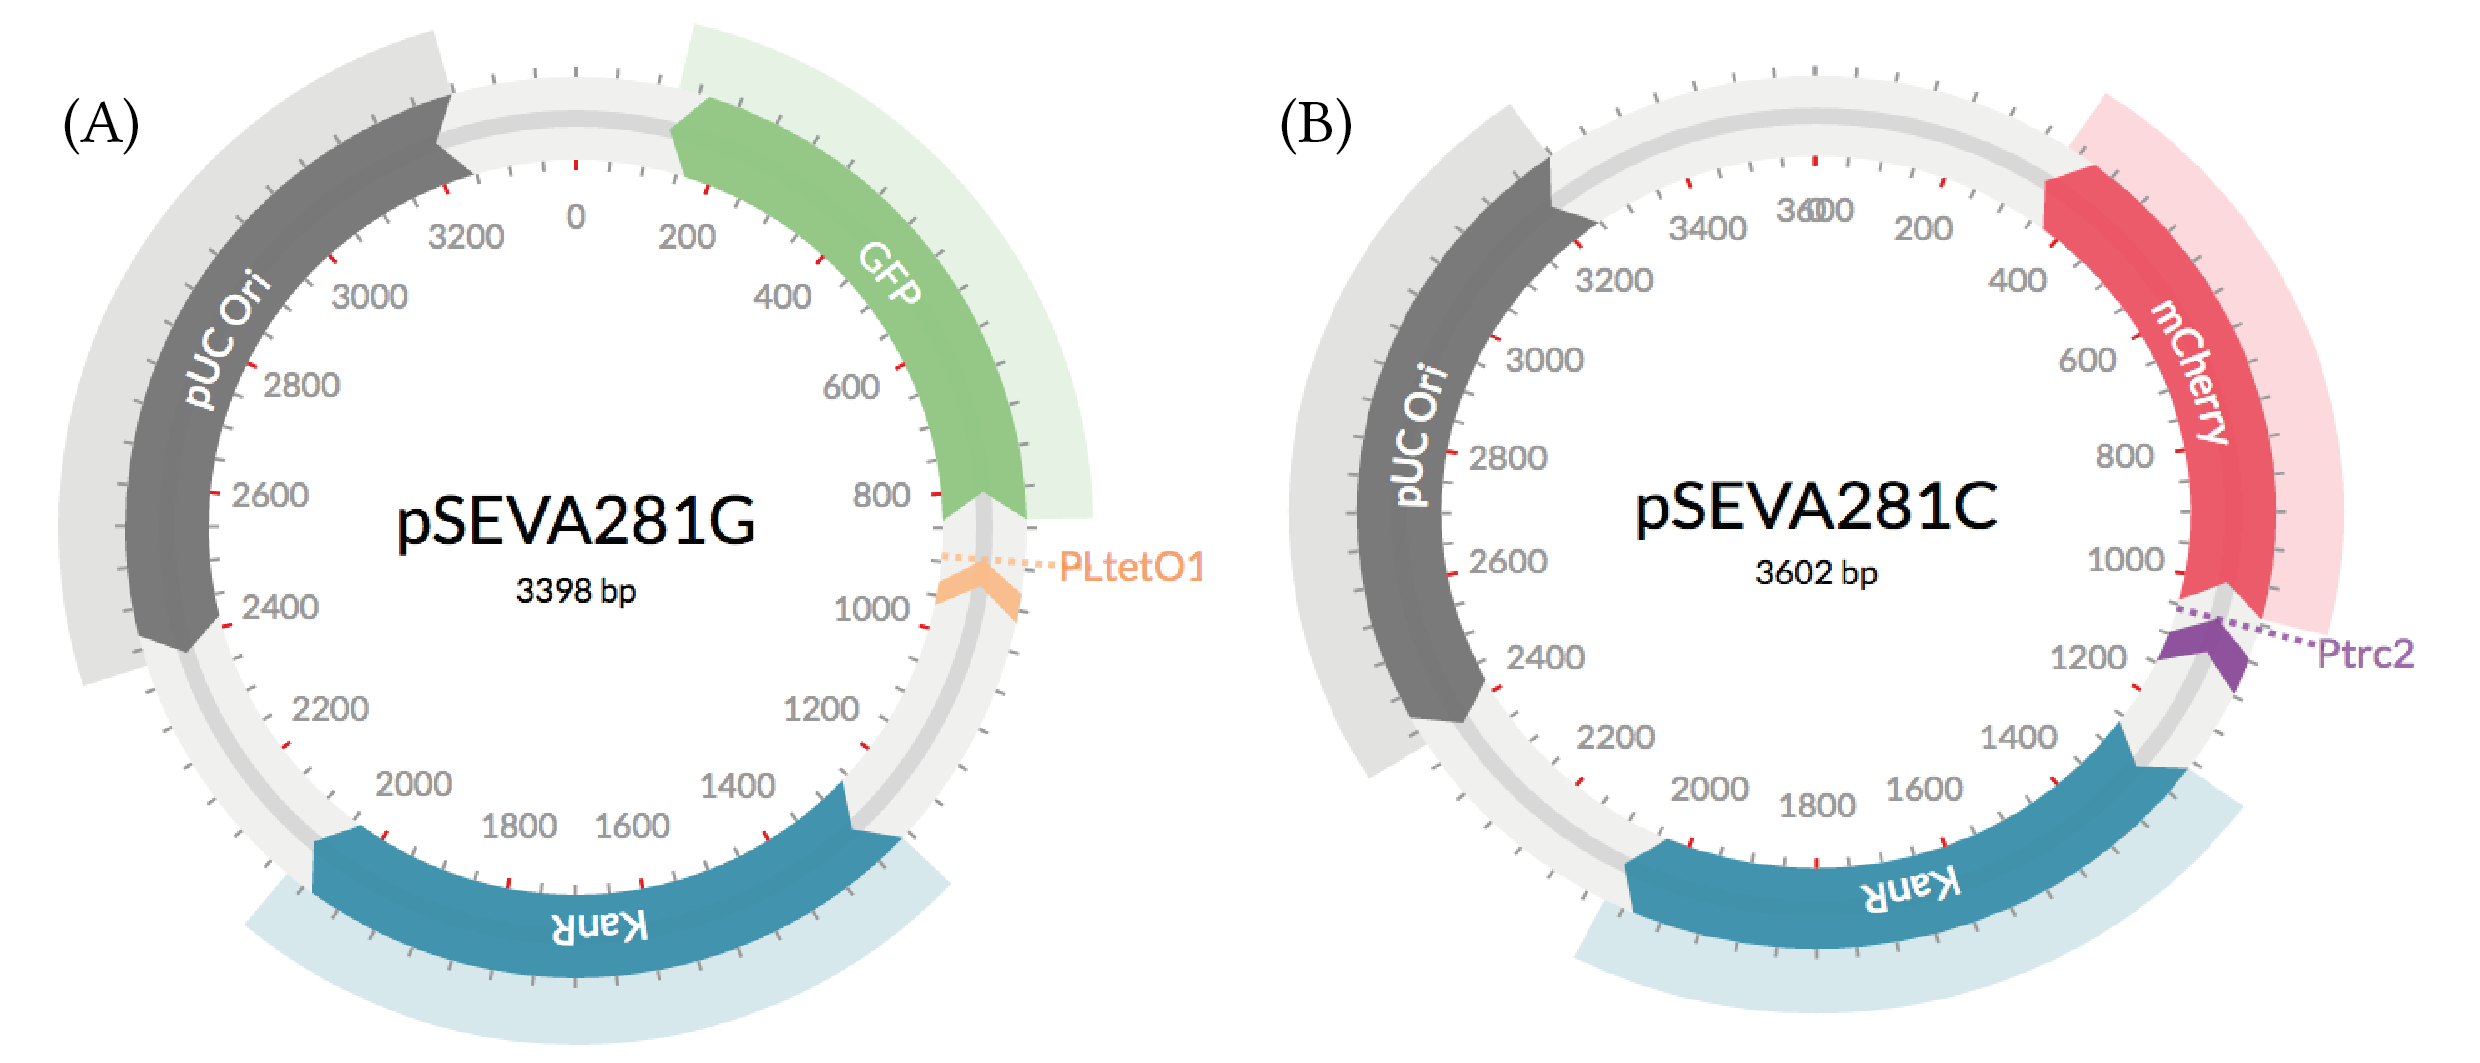
\includegraphics[width=\textwidth]{../../chapters/chapterABCFlow/images/plasmids_constructed.png}
		\caption[pSEVA281G and pSEVA281C plasmid map]{\label{fig:psevas}: The plasmids used to calibrate GFP and mCherry fluorescence. (A) pSEVA281G plasmid map (B) pSEVA281C plasmid map.  }
	\end{center}
\end{figure*}


\subsubsection{Growth rate investigation}

I carried out a growth rate analysis to determine whether the \acrshort{atc} or \acrshort{iptg} added to pKDL071 or pSEVA281G \textit{E. coli} cultures affected the growth of the bacteria. Cultures were grown without any inducer overnight as described in Section~\ref{sec:growth_meth}. Assays for the cultures were ran with and without added inducers. As can be seen in Figure~\ref{fig:growth_curve}, there is no difference between the conditions. The addition of either \acrshort{atc} or \acrshort{iptg} does not affect the growth rate of \textit{E. coli} K-12 MG1655. Additionally, \acrshort{atc} does not affect the growth rate of \textit{E. coli} DH5α. Since the addition of \acrshort{atc} flips the switch to the GFP high state, and \acrshort{iptg} to the mCherry high state, we can also conclude that the growth rate of the chassis is not affected by which side of the switch is in the high state. The growth rate of \textit{E. coli} DH5α was consistently lower than that of \textit{E. coli} K-12 MG1655.

\begin{figure*}[htbp]
	\begin{center}
		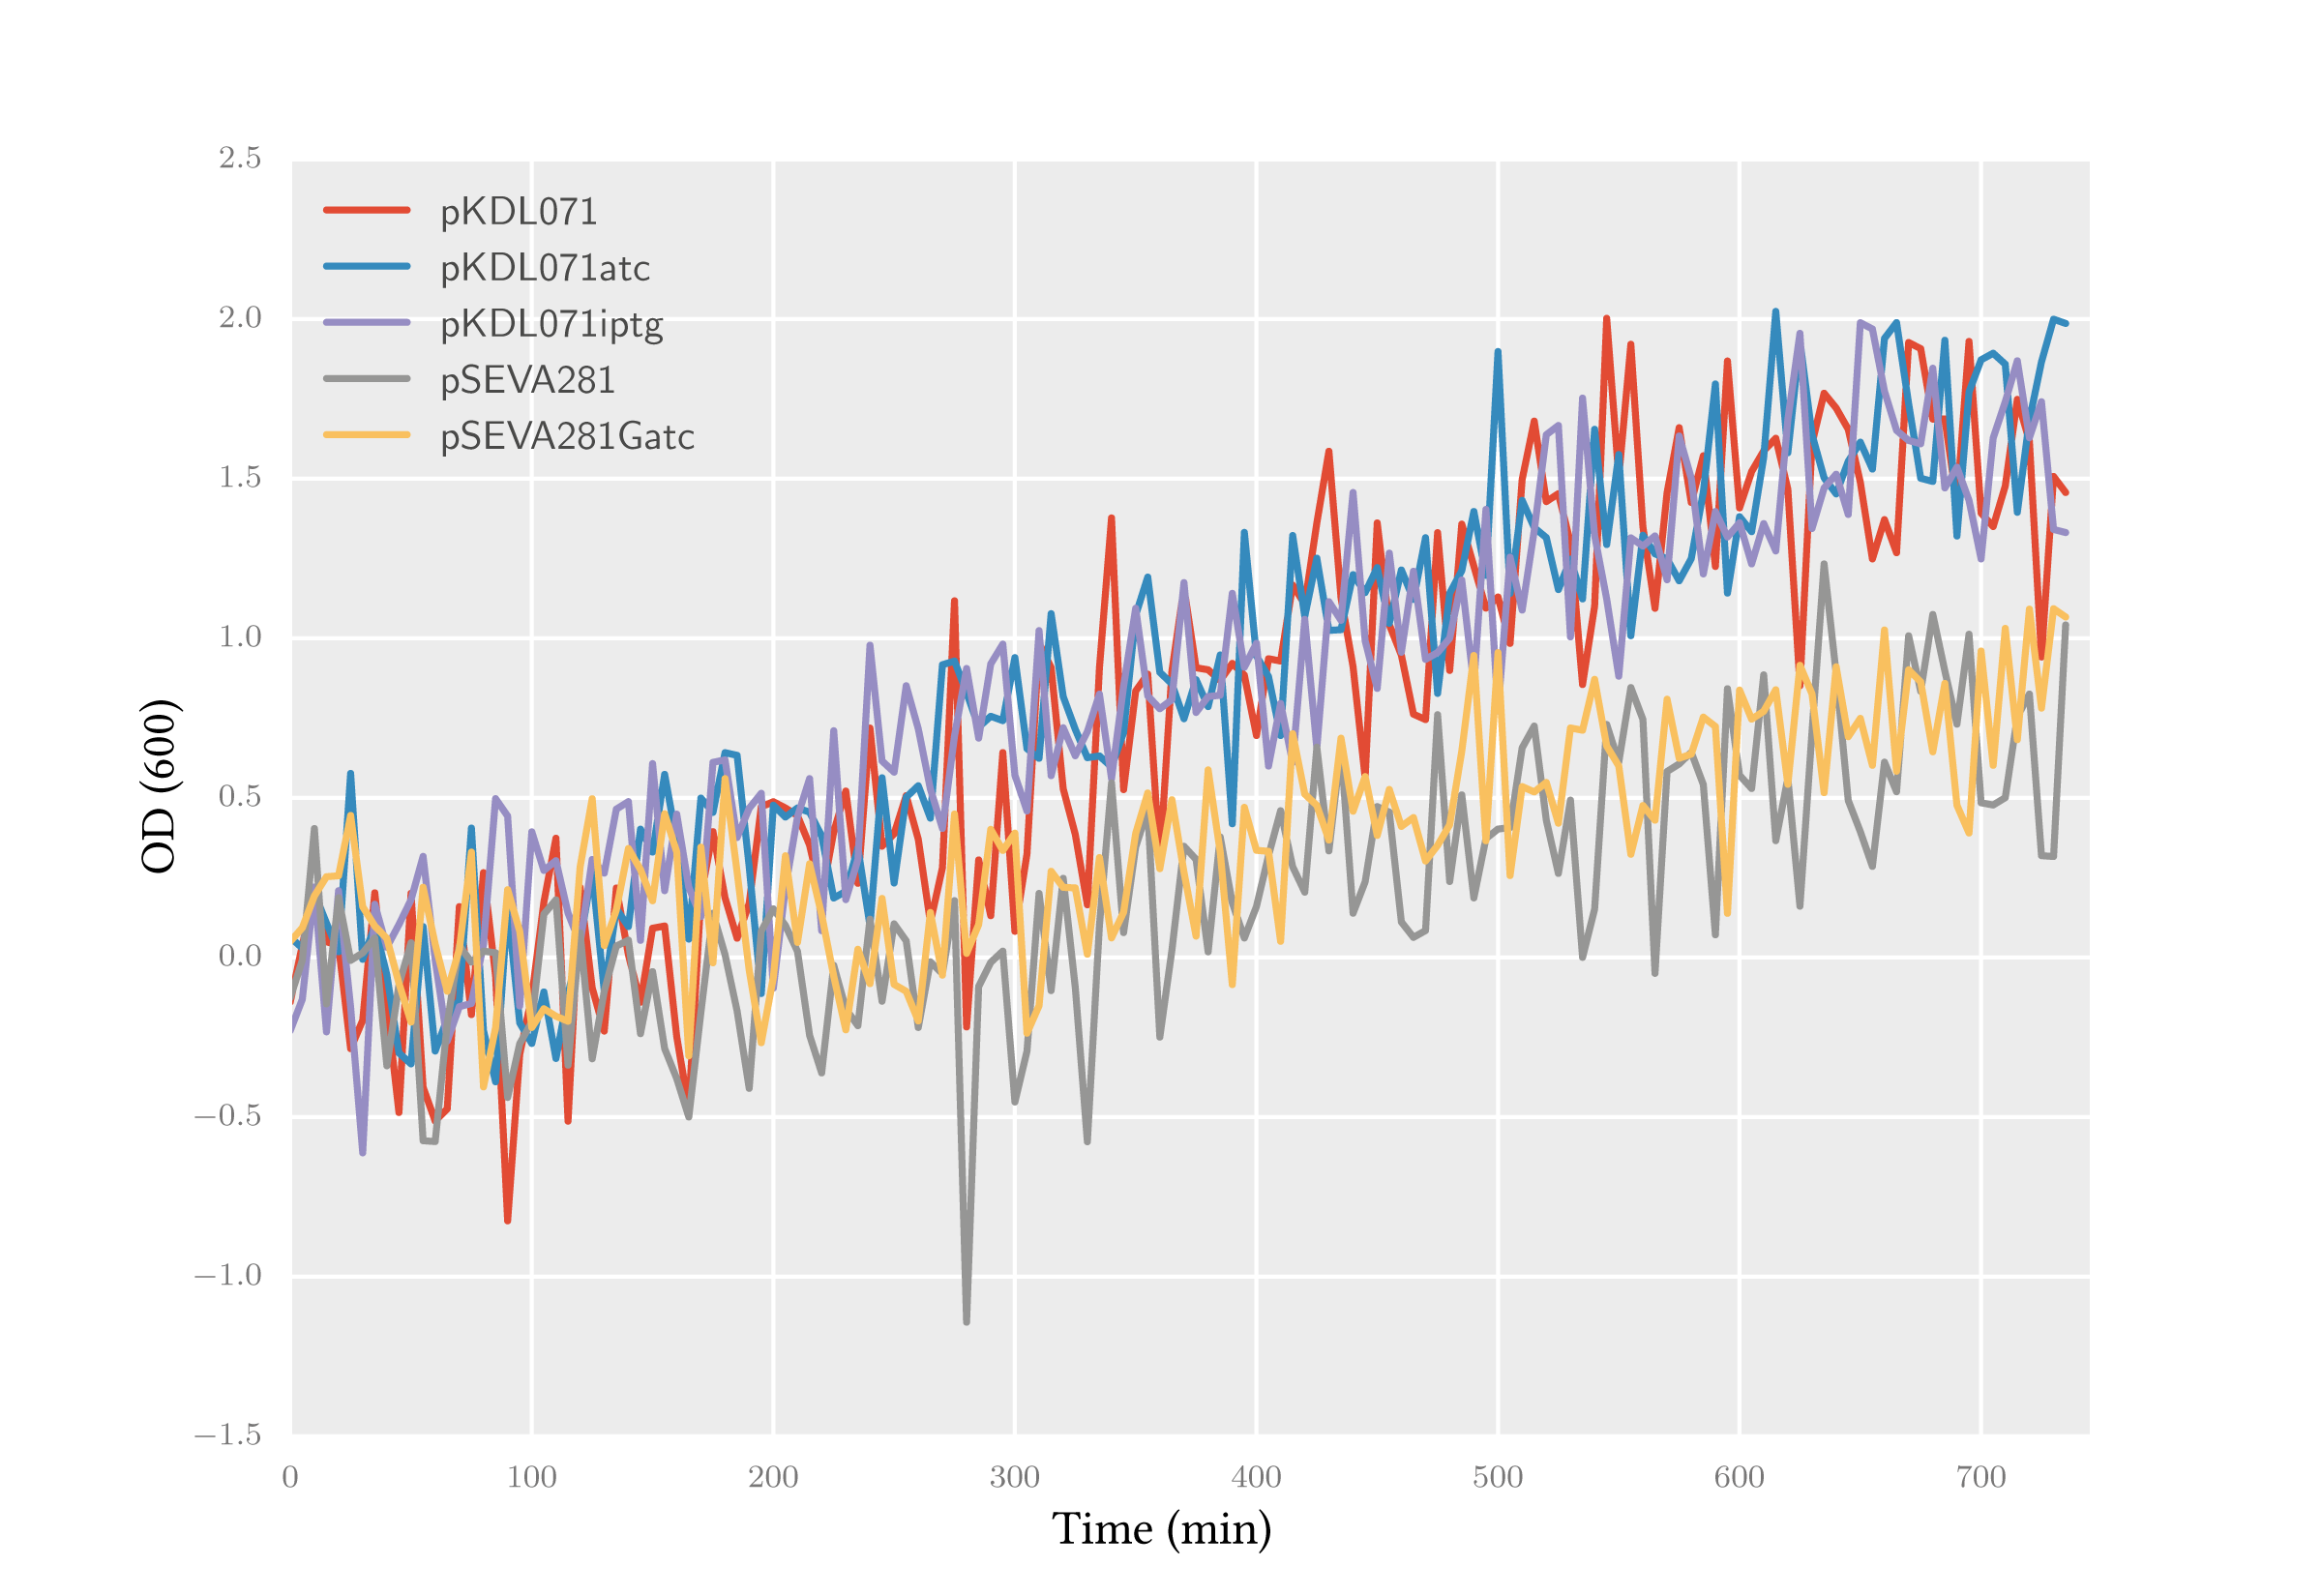
\includegraphics[scale=0.6]{../../chapters/chapterABCFlow/images/growth_curves.png}
		\caption[Growth rate curves of cultures with and without inducers]{\label{fig:growth_curve} Growth rate analysis of \textit{E. coli} K-12 MG1655 pKDL071 and \textit{E. coli} DH5α pSEVA281G cultures with and without inducers. The inducers do not affect the growth of the bacteria. }
	\end{center}
\end{figure*}

\clearpage



\subsubsection{Toggle switch concentration assays}

I carried out a concentration assay using flow cytometry, as described in Section~\ref{sec:flo_conc}. As can be seen in Figure~\ref{fig:switch_concent2d1d}A, during \acrshort{atc} induction the switch flips to a GFP high state when \acrshort{atc} concentration is at \SI{0.09}{\nano\gram\per\milli\liter} or higher. We observe a bimodal distribution at concentrations \SI{0.07}{\nano\gram\per\milli\liter} and \SI{0.08}{\nano\gram\per\milli\liter} close to the instantaneous switching point (at \SI{0.09}{\nano\gram\per\milli\liter}) where noise creates two simultaneous states. Therefore we observe part of the population switched to the GFP high state. In the case of \acrshort{iptg} induction (Figure~\ref{fig:switch_concent2d1d}B) we find that the switch flips to the mCherry high state when the concentration of \acrshort{iptg} is higher or equal to 0.001M. A decrease in GFP fluorescence is also observed. We do not observe a bimodal distribution in this case. The Hill functions for repression and activation wer used to obtain the characterisation curves of the two inductions, \acrshort{atc} and \acrshort{iptg} and are given below. 

\begin{figure*}[htbp]
	\begin{center}
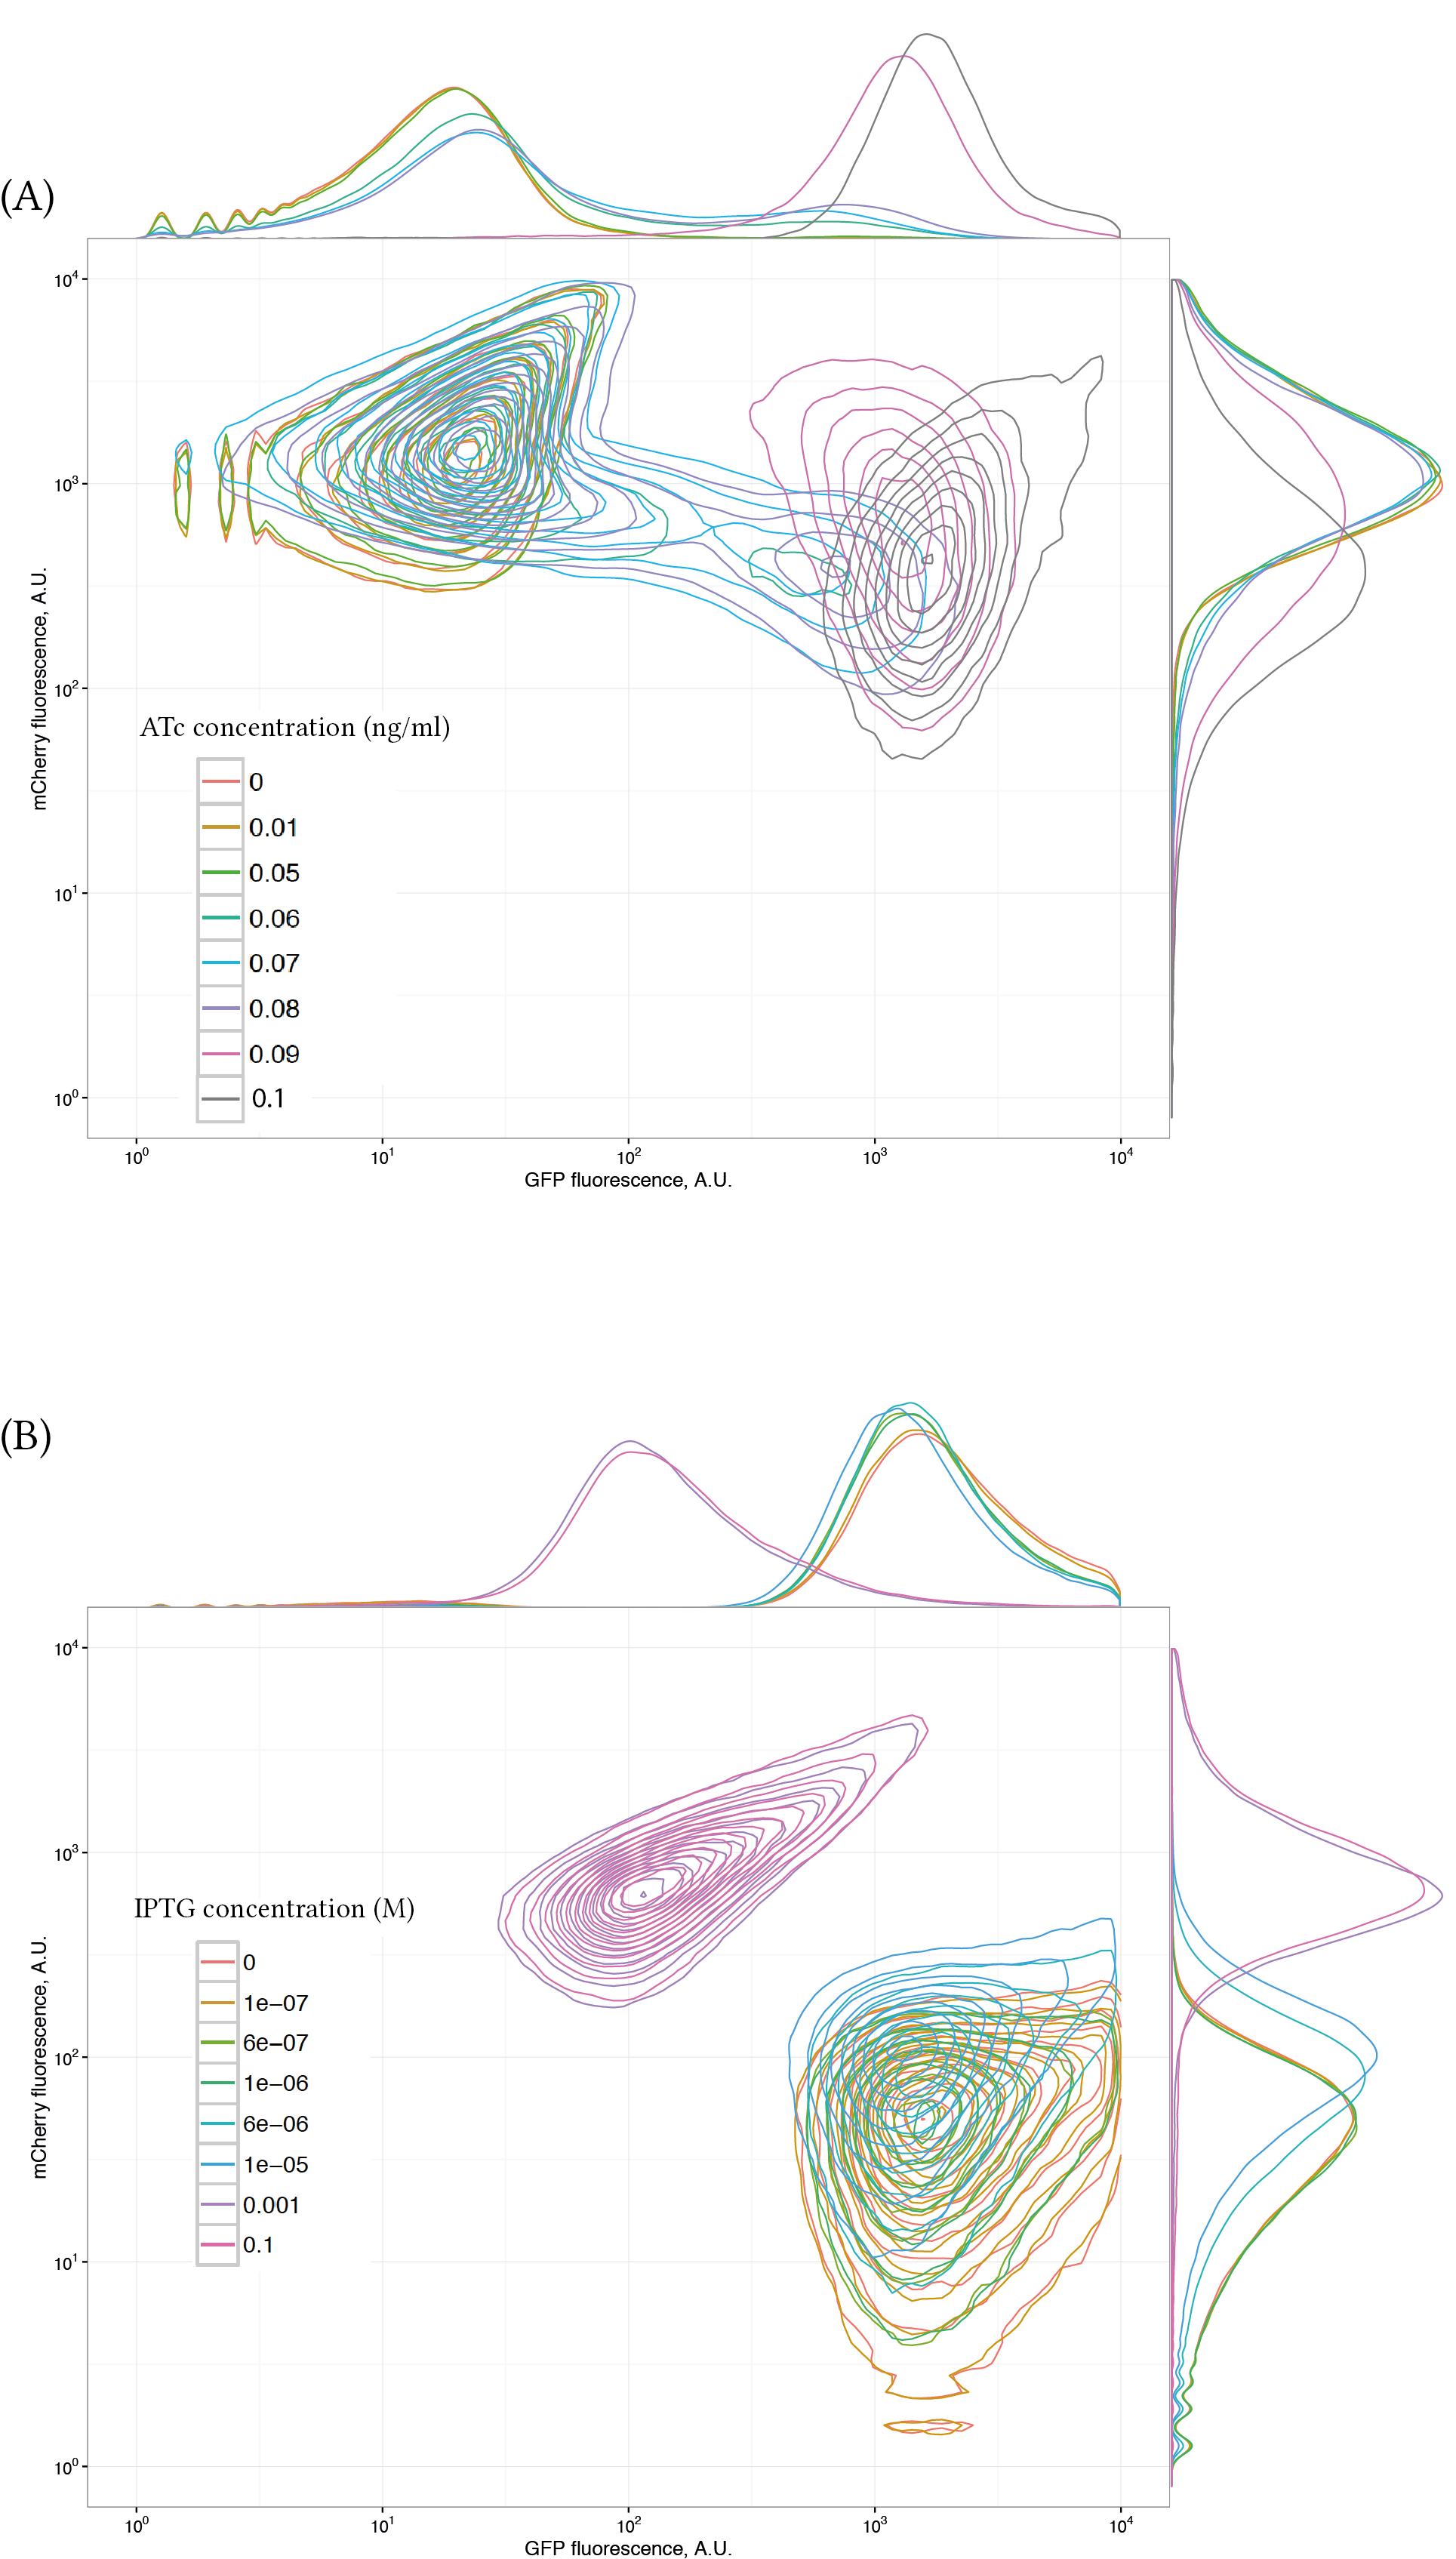
\includegraphics[scale=0.7]{../../chapters/chapterABCFlow/images/pKDL071_concentrations_2d1d.png}
\caption[Inducer concentration assay of pKDL071]{\label{fig:switch_concent2d1d}(A) \acrshort{atc} induction at various concentrations (B) \acrshort{iptg} induction at various concentrations. }
\end{center}
\end{figure*}


\begin{align}
 	F_{act} = P_{min} + (P_{max} - P_{min})\frac{\Big(\frac{[I]}{Kd}\Big)^n}{1+\Big(\frac{[I]}{Kd}\Big)^n},\\
 	F_{rep} = P_{max} + (P_{min} - P_{max})\frac{(1)}{1+\Big(\frac{[I]}{Kd}\Big)^n}
\end{align}
 
\noindent where F is the median fluorescent unit and [I] is the concentration of inducer. $P_{min}$ and $P_{max}$ are the minimum and maximum fluorescence respectively, and Kd and n are the dissociation constant, and Hill coefficient. I fit the Hill function by using the nonlinear least squares estimation in the R statistical environment~\autocite{R:2008}. Initial values used for the Hill function parameters $P_{min}$, $P_{max}$, $Kd$, and $n$ are given in Table~\ref{tab:hill_initial}.



%\begin{table}[htbp]
%\centering
%\caption{Initial values used for Hill function parameters}
%\label{tab:hill_initial}
%\begin{tabular}{@{}lllll@{}}
%\toprule
% & pmin & pmax & kd & n \\ \midrule
%ATc induction & 18 & 1800 & 0.12 & 2 \\
%IPTG induction & 0 & 800 & 0.00001 & 1.6 \\ \bottomrule
%\end{tabular}
%\end{table}

\begin{table}[htbp]
\centering
\caption{Inferred values from the Hill equations in \acrshort{atc} and \acrshort{iptg} inductions}
\label{tab:hill_initial}
\begin{tabular}{@{}lllll@{}}
\toprule
\multirow{2}{*}{Parameters} & \multicolumn{2}{l}{\acrshort{atc} induction} & \multicolumn{2}{l}{IPTG induction} \\ \cmidrule(l){2-5} 
 & GFP & mCherry & GFP & mCherry \\ \midrule
pmin & 18.3 & 330.45 & 139.69 & 7.3 \\
pmax & 1541.3 & 974.46 & 1392.822 & 687.3 \\
kd & 0.097 & 0.09917 & 0.000019 & 0.00012\\
n & 56.7 & 135.006 & 2.59 & 0.98\\ 
fold change & 84.1 & 2.94 & 9.97 & 94.15 \\ \bottomrule
\end{tabular}
\end{table}

\begin{figure*}[tb]
	\begin{center}
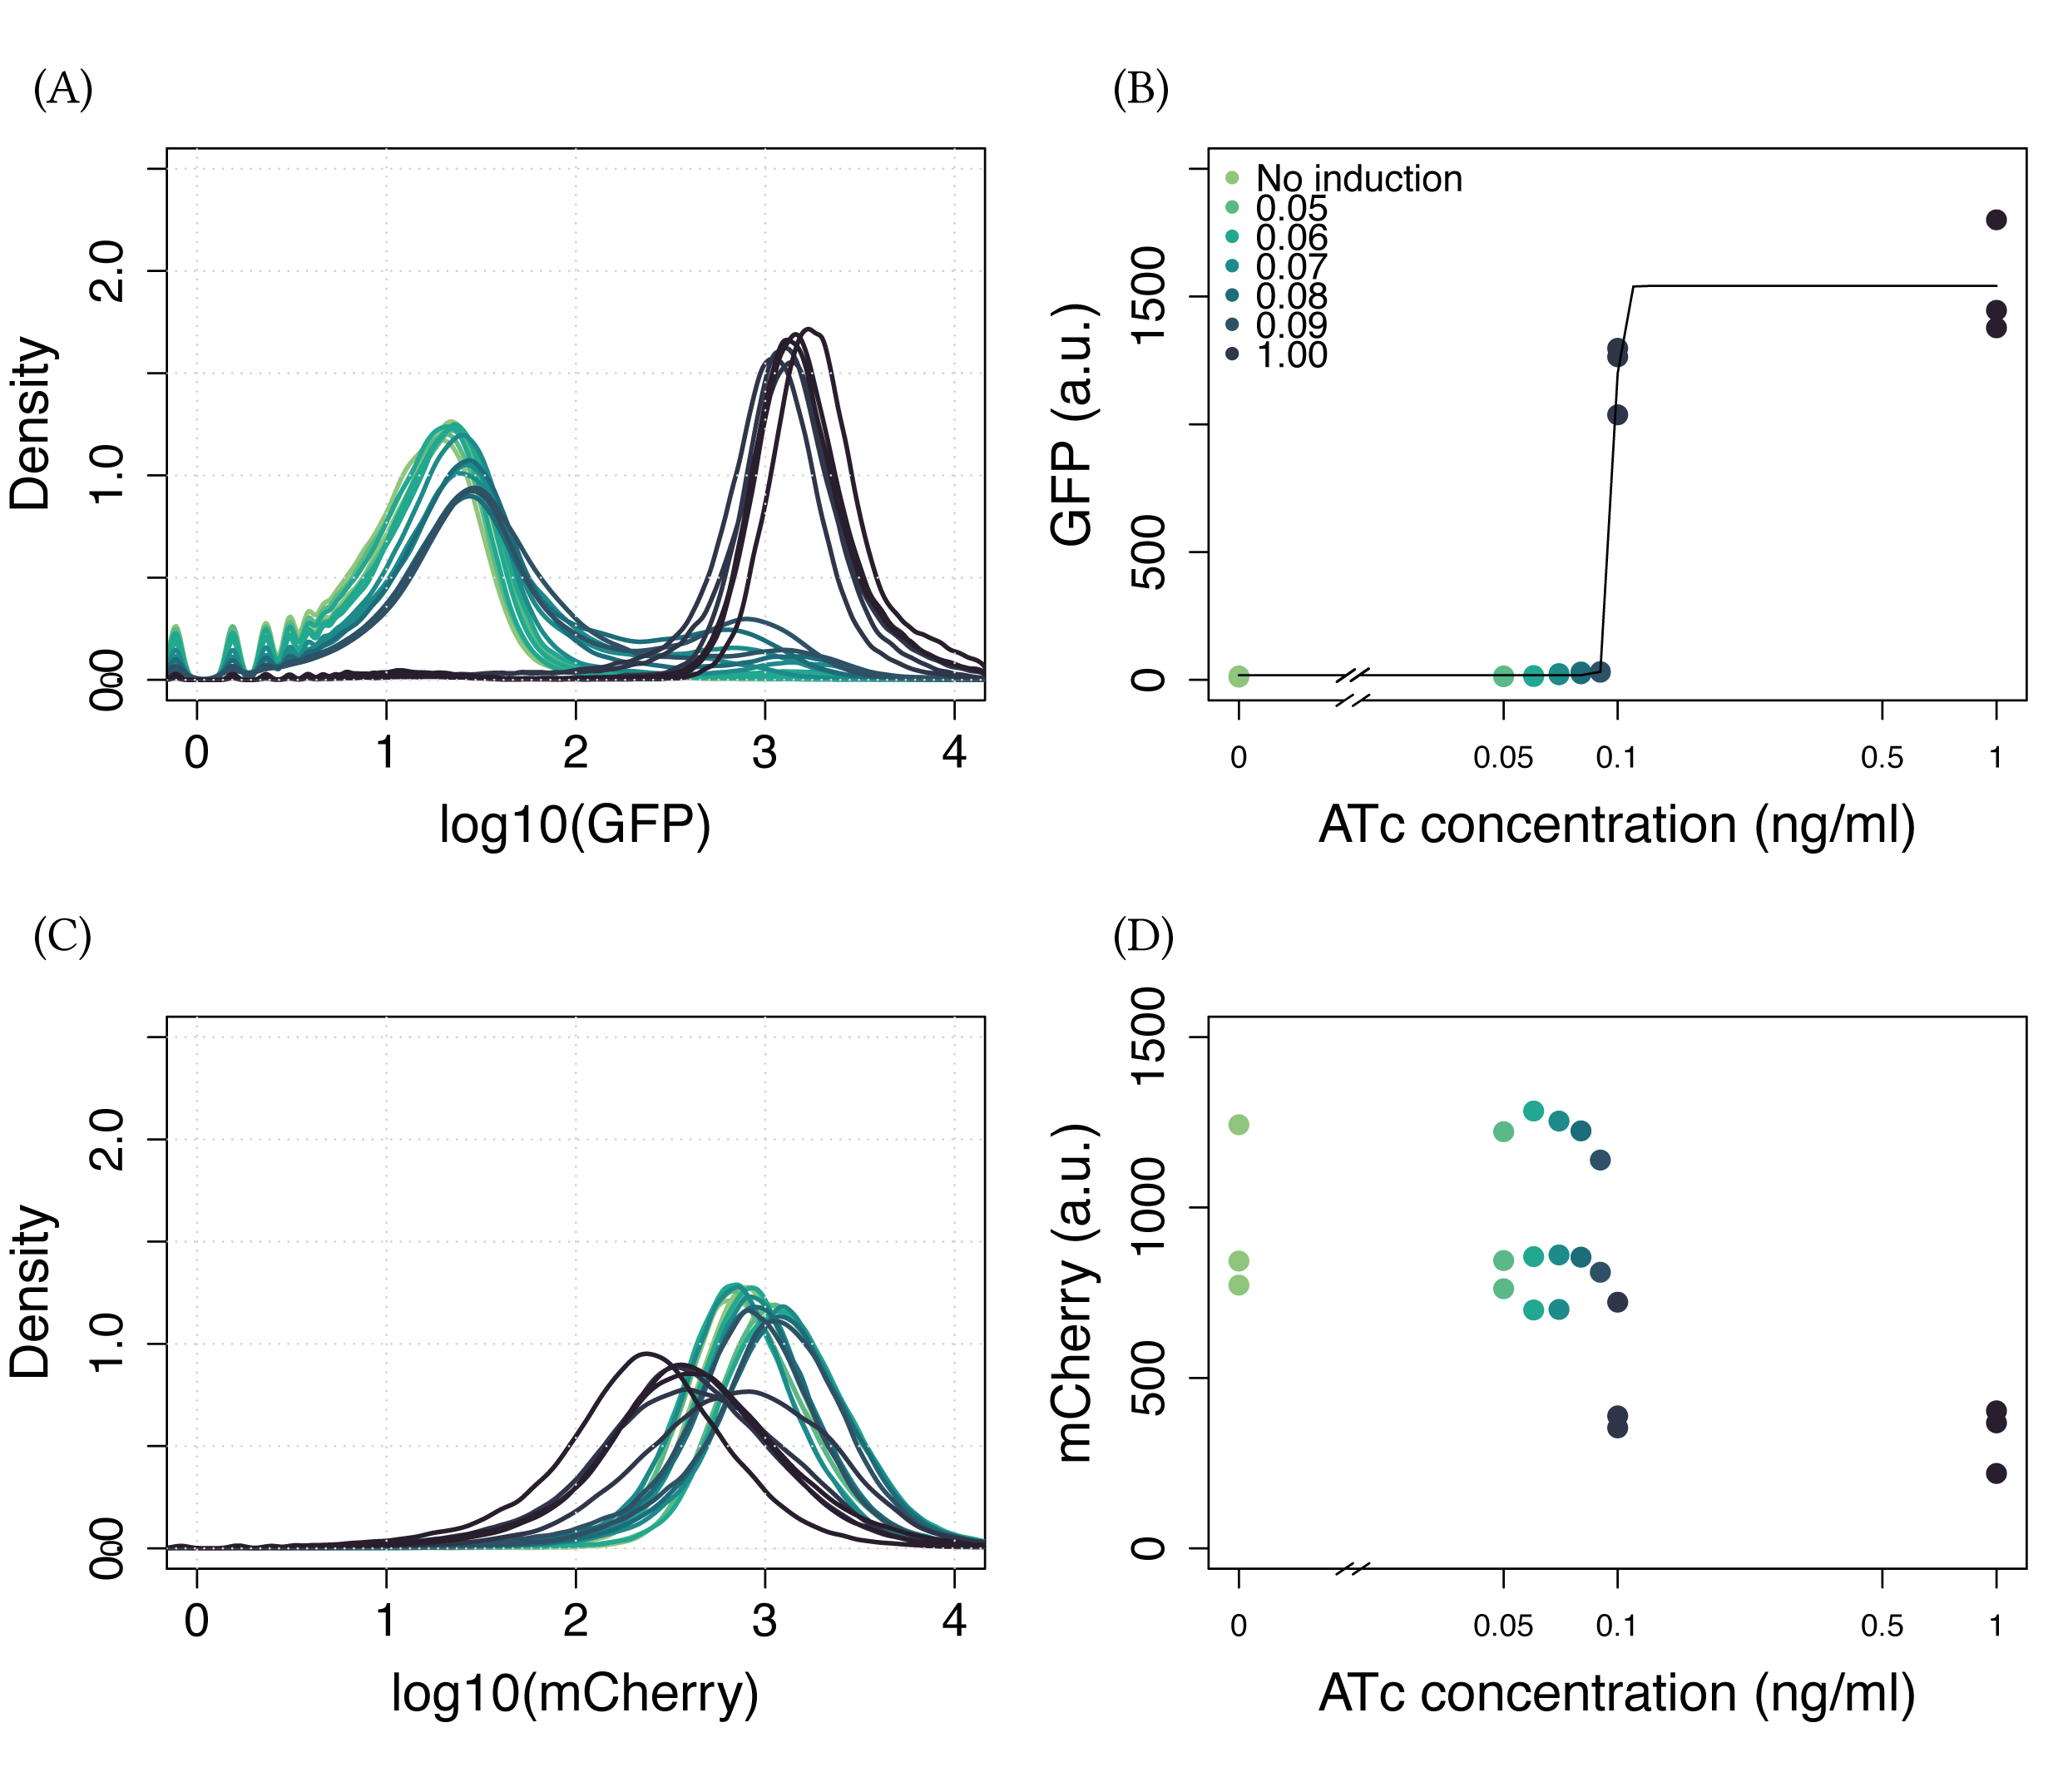
\includegraphics[width=\textwidth]{../../chapters/chapterABCFlow/images/pKDL071_concentrations_ATc-01.png}
\caption[Characterisation of pKDL071 after \acrshort{atc} induction]{\label{fig:switch_concentrations_model_atc} (A) Flow cytometry density plots of the logged GFP fluorescence obtained for each \acrshort{atc} induction. (B) There is an 84.1 fold increase in GFP fluorescence with increasing \acrshort{atc} concentration. (C) Flow cytometry density plots of the logged mCherry fluorescence obtained for each \acrshort{atc} induction. (D) The medians of the flow cytometry densities of the triplicates of \acrshort{atc} induction. We observe a decrease in mCherry fluorescence.}
\end{center}
\end{figure*}

For the case of the \acrshort{atc} induction we observe a sharp switch between the GFP low to the GFP high state, as well as between the mCherry high to the mCherry low states, as can be seen in the characterisation curves in Figure~\ref{fig:switch_concentrations_model_atc}B and D. This sharp switch made the fitting of the Hill function challenging. The parameters producing the best fit of the Hill function found are given in Table~\ref{tab:hill_initial}. The cooperativity parameter n is very high in this model, in order to be able to fit the data collected. This could be caused by discontinuous switching, which would mean that the Hill function is not appropriate for modelling its behaviour. 

%We observe a 84.1 fold increase in GFP fluorescence. We also observe a decrease in mCherry fluorescence during \acrshort{atc} induction. The dynamical range of GFP is larger than the dynamical range of mCherry during \acrshort{atc} induction.s



\begin{figure*}[tb]
	\begin{center}
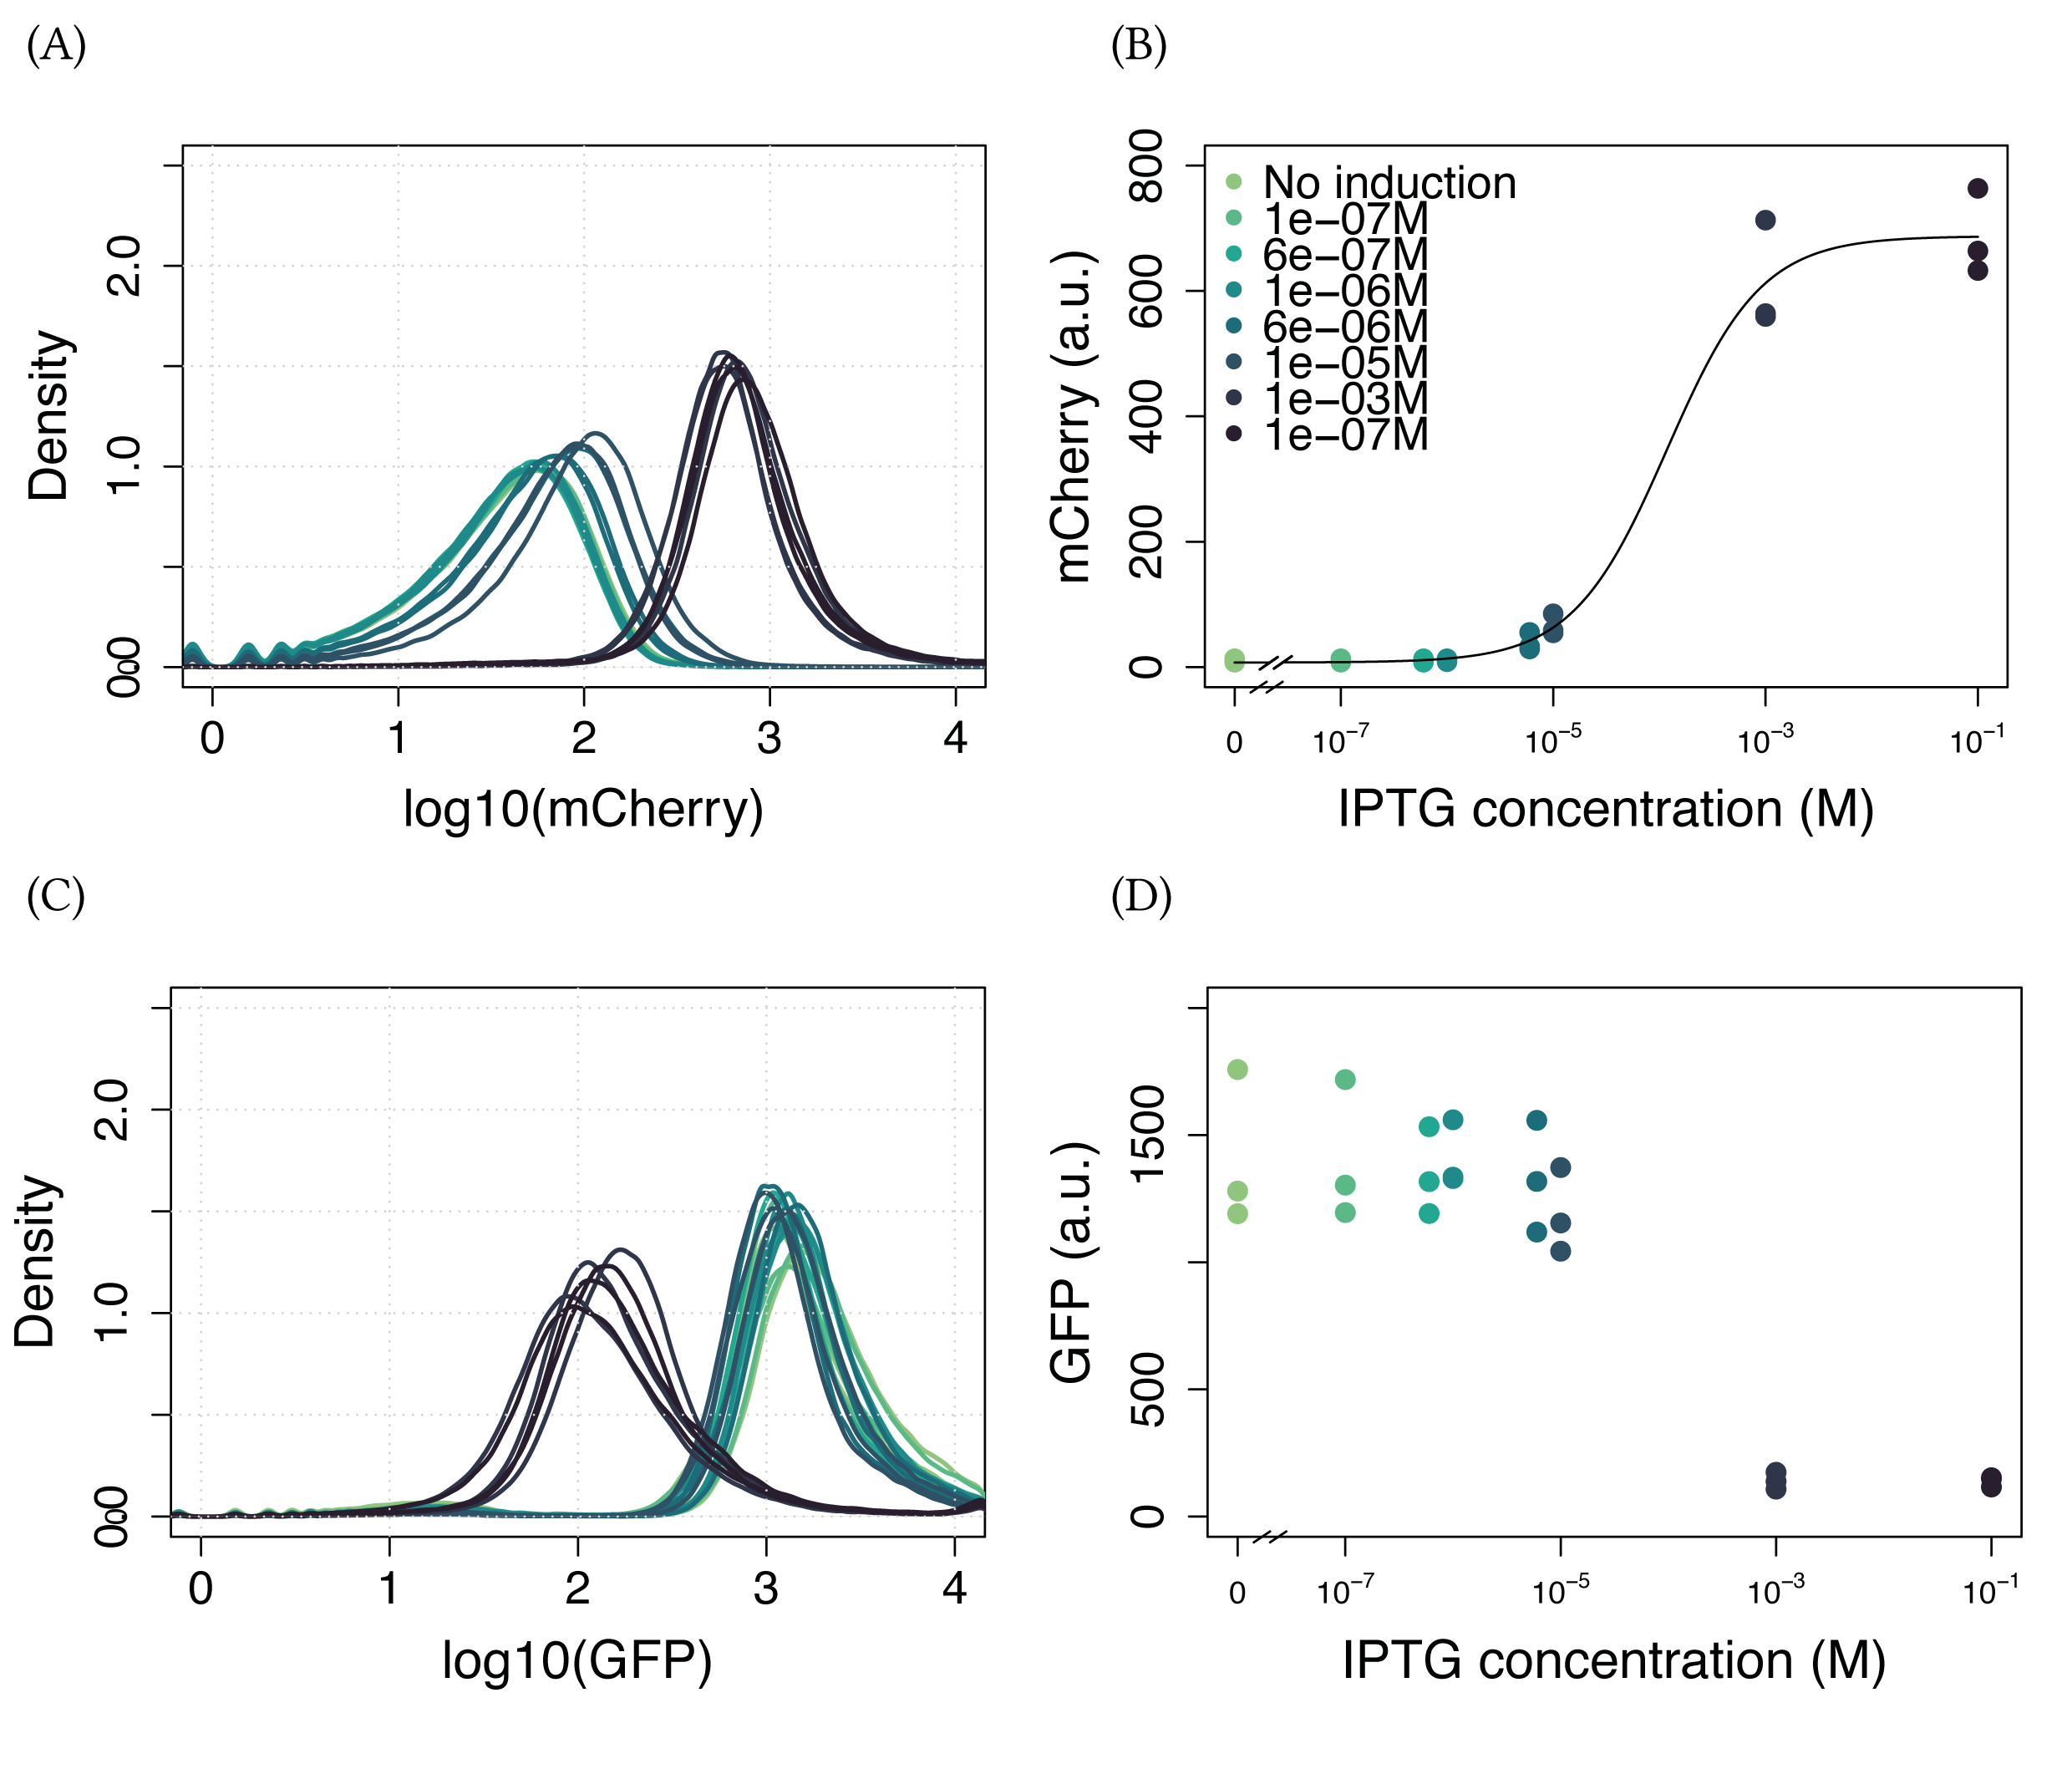
\includegraphics[width=\textwidth]{../../chapters/chapterABCFlow/images/pKDL071_concentrations_model_fit-01.png}
\caption[Characterisation of pKDL071 after \acrshort{iptg} induction]{\label{fig:switch_concentrations_model} (A) Flow cytometry density plots of the logged mCherry fluorescence obtained for each IPTG induction. (B) There is a 94.5 fold increase in mCherry fluorescence with increasing \acrshort{iptg} concentration. (C) Flow cytometry density plots of the logged GFP fluorescence obtained for each IPTG induction. (D) The medians of the flow cytometry densities of the triplicates of IPTG induction. We observe a decrease in GFP fluorescence.}
\end{center}
\end{figure*}


During IPTG induction we observe an increase in mCherry fluorescence, as seen in Figure~\ref{fig:switch_concentrations_model}. The parameters obtained via the nonlinear least squares estimation are given in Table~\ref{tab:hill_initial}. There is a 94.5 fold increase in mCherry fluorescence.  We also observe a decrease in GFP fluorescence with increasing IPTG concentrations. 

Figures~\ref{fig:switch_concentrations_model_atc} and~\ref{fig:switch_concentrations_model} demonstrate that the genetic toggle switch present on the pKDL071 plasmid is capable of behaving like a switch. By adding the appropriate inducers at increasing concentrations I observed the switch flipping between its two states, GFP high/mCherry low and GFP low/mCherry high. I observed a bigger fold increase in fluorescence in mCherry during IPTG inductions compared to GFP during \acrshort{atc} inductions. Both inductions resulted in a large overall change in fluorescence for the two fluorescent proteins GFP and mCherry. 


\subsubsection{Toggle switch time course assay}
\label{sec:ts_time}
I further analysed the pKDL071 toggle switch by investigating the time it takes for it to switch from one high state to the other. To do that I used the method outlined in Section~\ref{sec:flo_time}. I obtained separate time courses for the \acrshort{iptg} and \acrshort{atc} inductions. 

As can be seen in Figure~\ref{fig:switch_timecourse_atc} pKDL071 \acrshort{atc}  induction begins switching 1 hour after induction. Complete induction is seen at 6 hours. During the \acrshort{iptg} induction (Figure~\ref{fig:switch_timecourse_iptg}) we see a bimodal distribution at 4 hours, and induction is complete at 6 hours. We observe that during \acrshort{atc} induction there is an increase in \acrshort{gfp} fluorescence and a decrease in mCherry fluorescence, in the case of \acrshort{iptg} induction the increase in mCherry fluorescence is not as prominent. A decrease in GFP fluorescence is observed during \acrshort{iptg} induction. 

\begin{figure*}[tb]
	\begin{center}
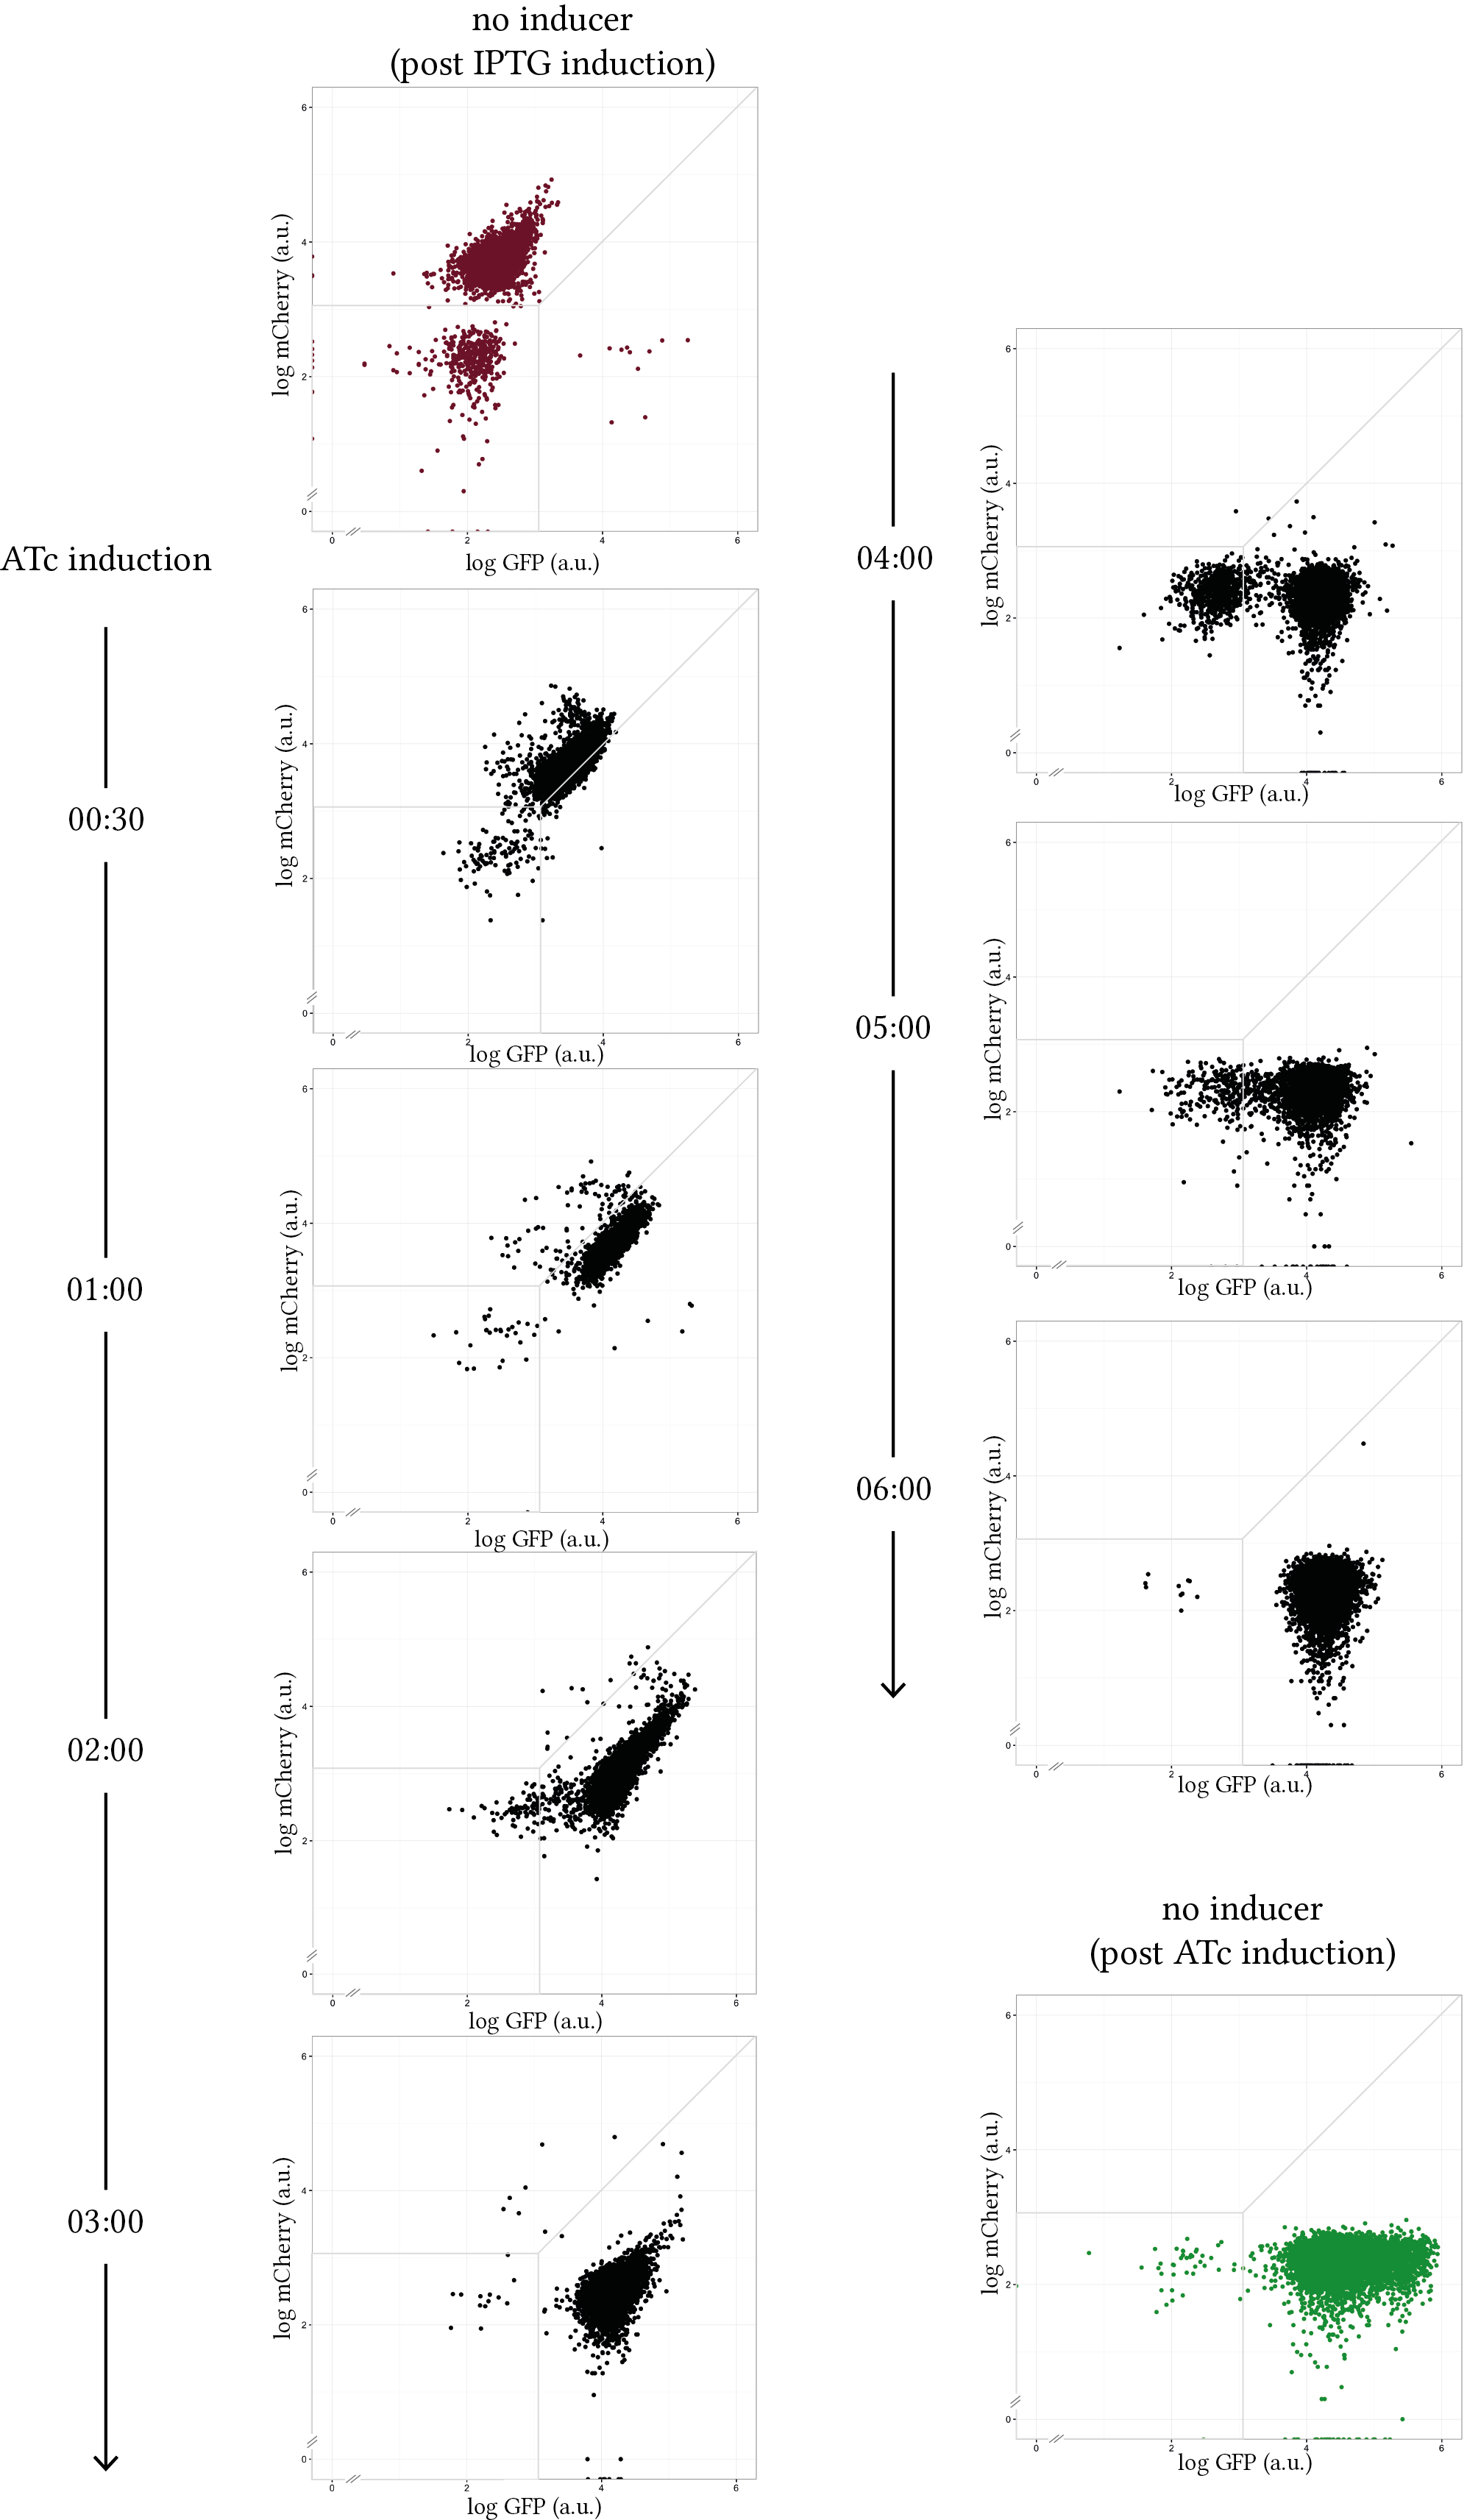
\includegraphics[scale=0.7]{../../chapters/chapterABCFlow/images/pKDL071_atc_time.png}
\caption[\acrshort{atc} induction of pKDL071 over time]{\label{fig:switch_timecourse_atc} \acrshort{atc} induction of pKDL071 over time}
\end{center}
\end{figure*}


\begin{figure*}[tb]
	\begin{center}
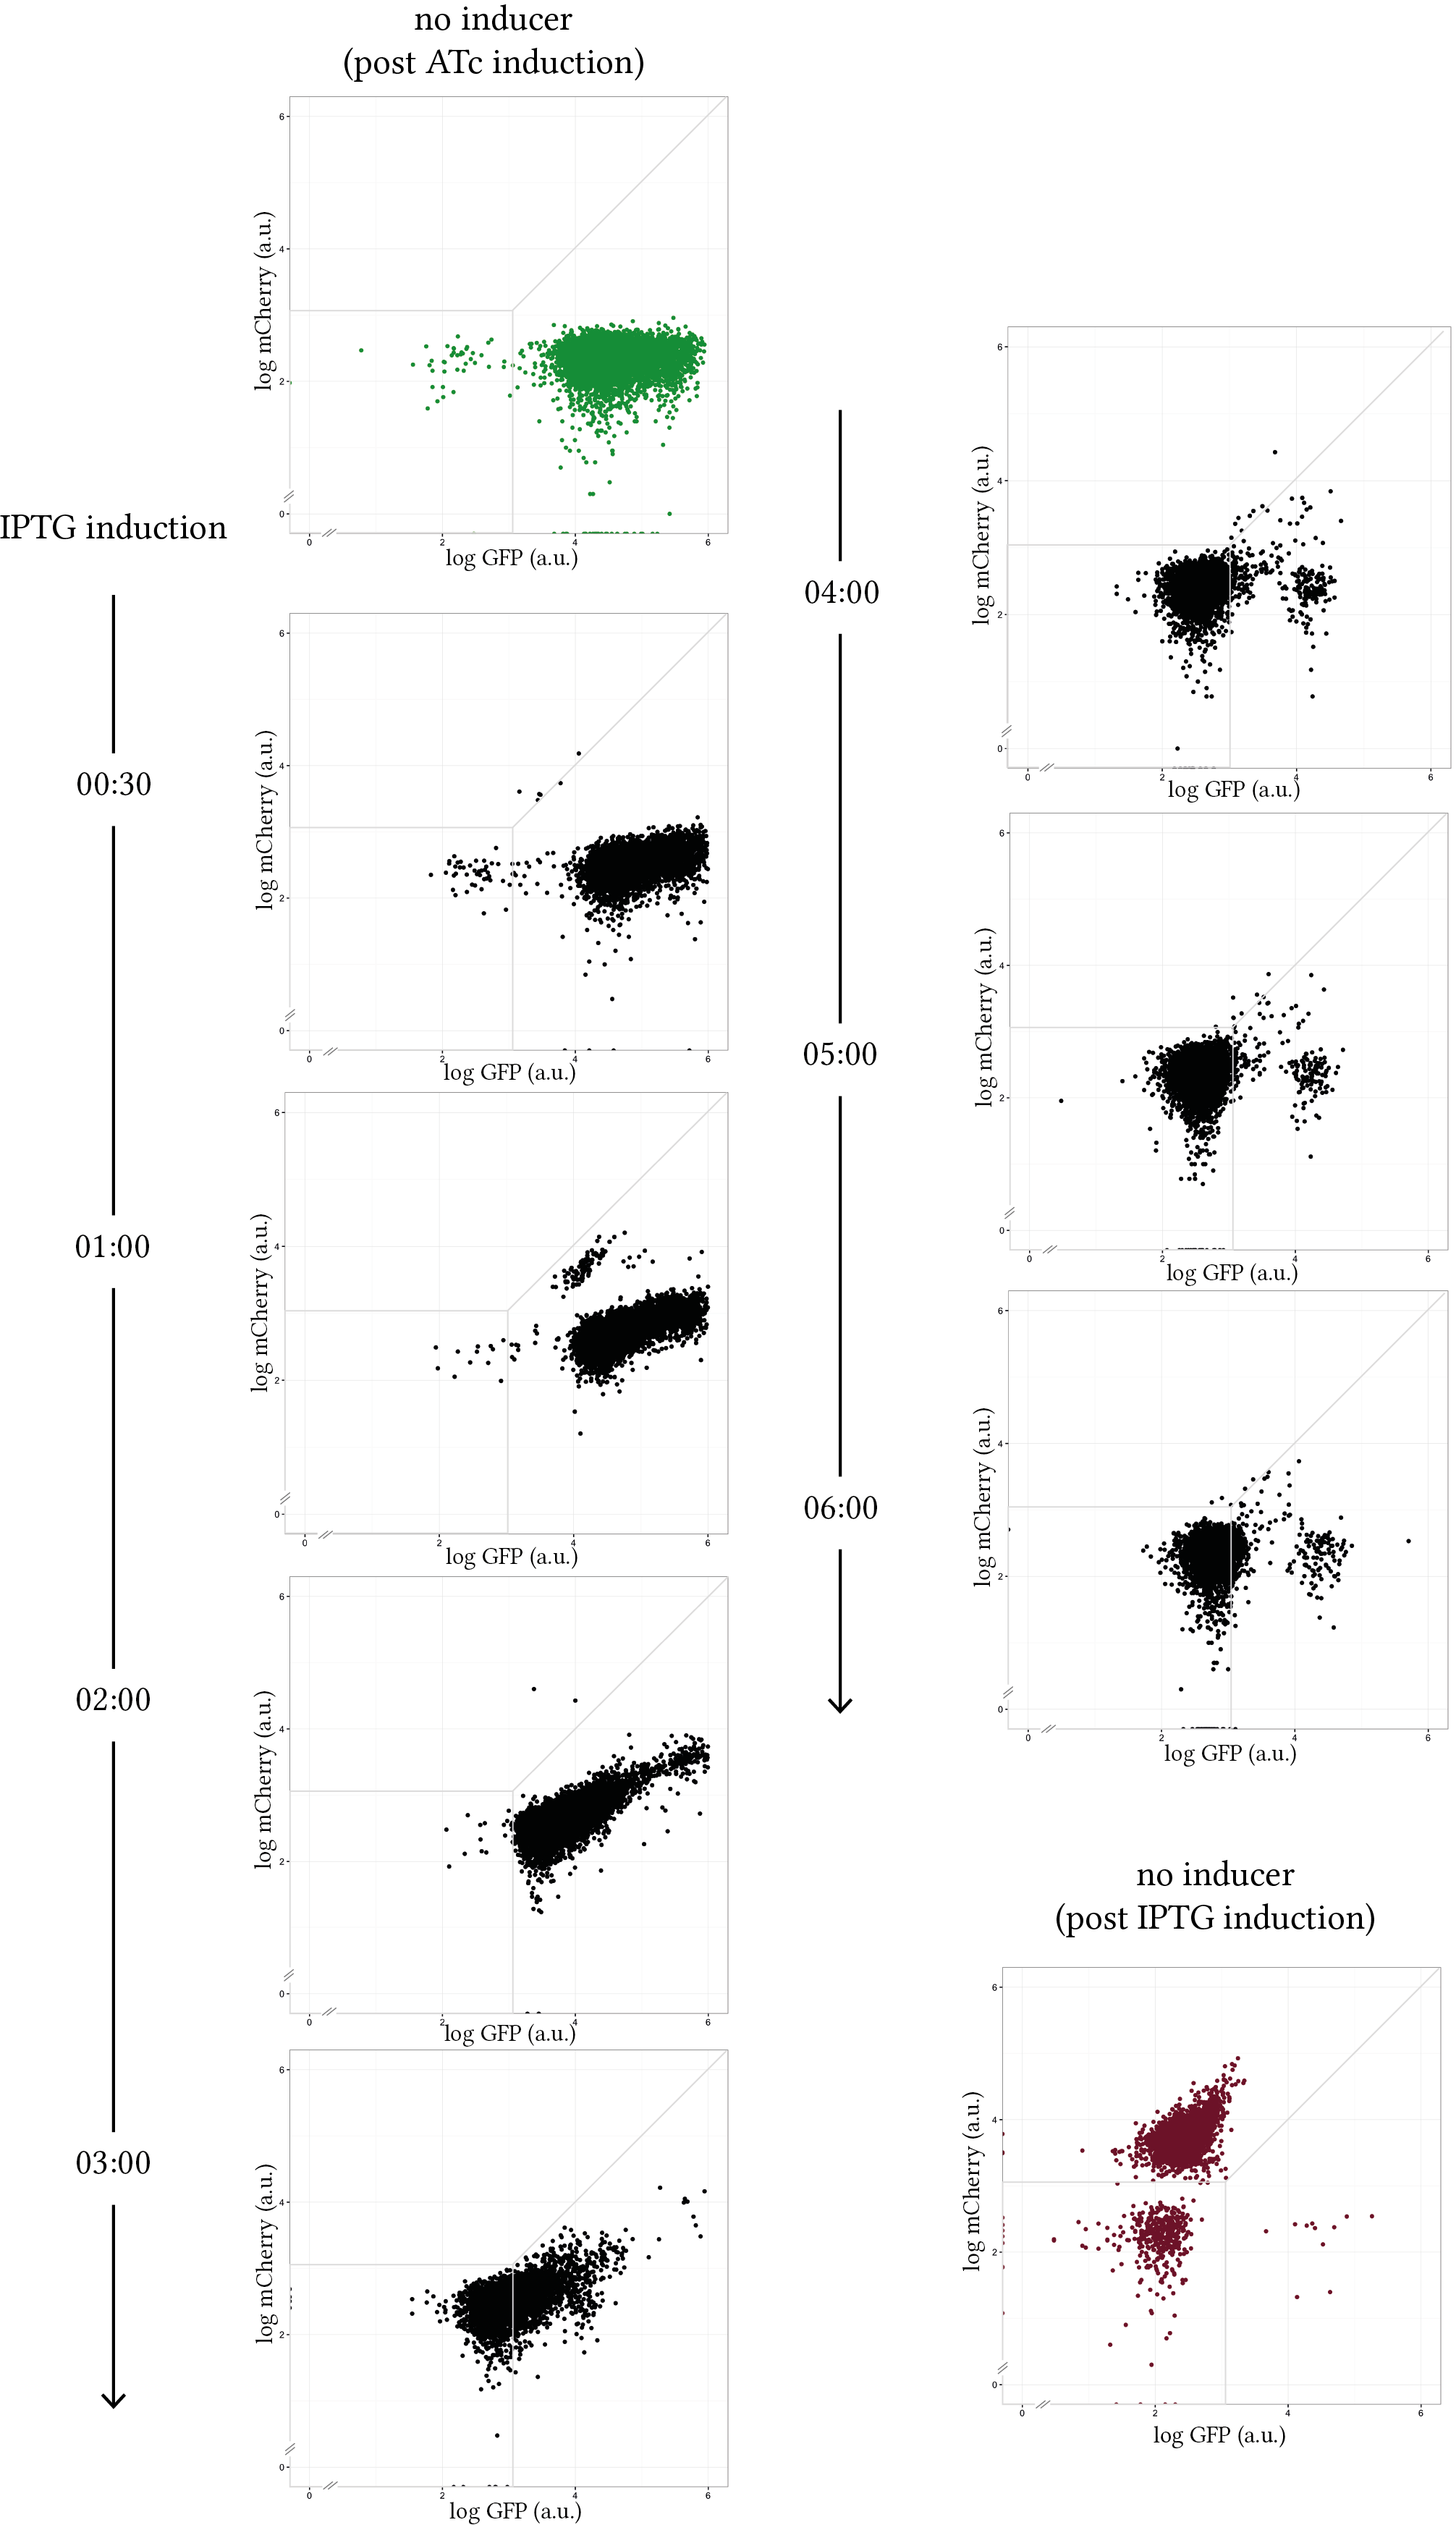
\includegraphics[scale=0.7]{../../chapters/chapterABCFlow/images/pKDL071_iptg_time.png}
\caption[\acrshort{iptg} induction of pKDL071 over time]{\label{fig:switch_timecourse_iptg} \acrshort{iptg} induction of pKDL071 over time}
\end{center}
\end{figure*}
\clearpage

In the next section I use ABC-Flow to fit a computational model to the time course data obtained. Prior to fitting a model to it, I process the data by removing the unresponsive populations. This ensures that the model is fitted only to the data from cells that respond to the inducers. As seen in Figure~\ref{fig:switch_timecourse_atc}, during the \acrshort{atc} induction there is an unresponsive population of cells where GFP and mCherry fluorescence are both less that $10^3$. This population is excluded from further analysis of the data. During the IPTG induction there is a population of cells that does not respond to the addition of IPTG by switching from GFP high to mCherry high. This population of cells is also excluded from further analysis. 

%\begin{figure*}[tb]
%	\begin{center}
%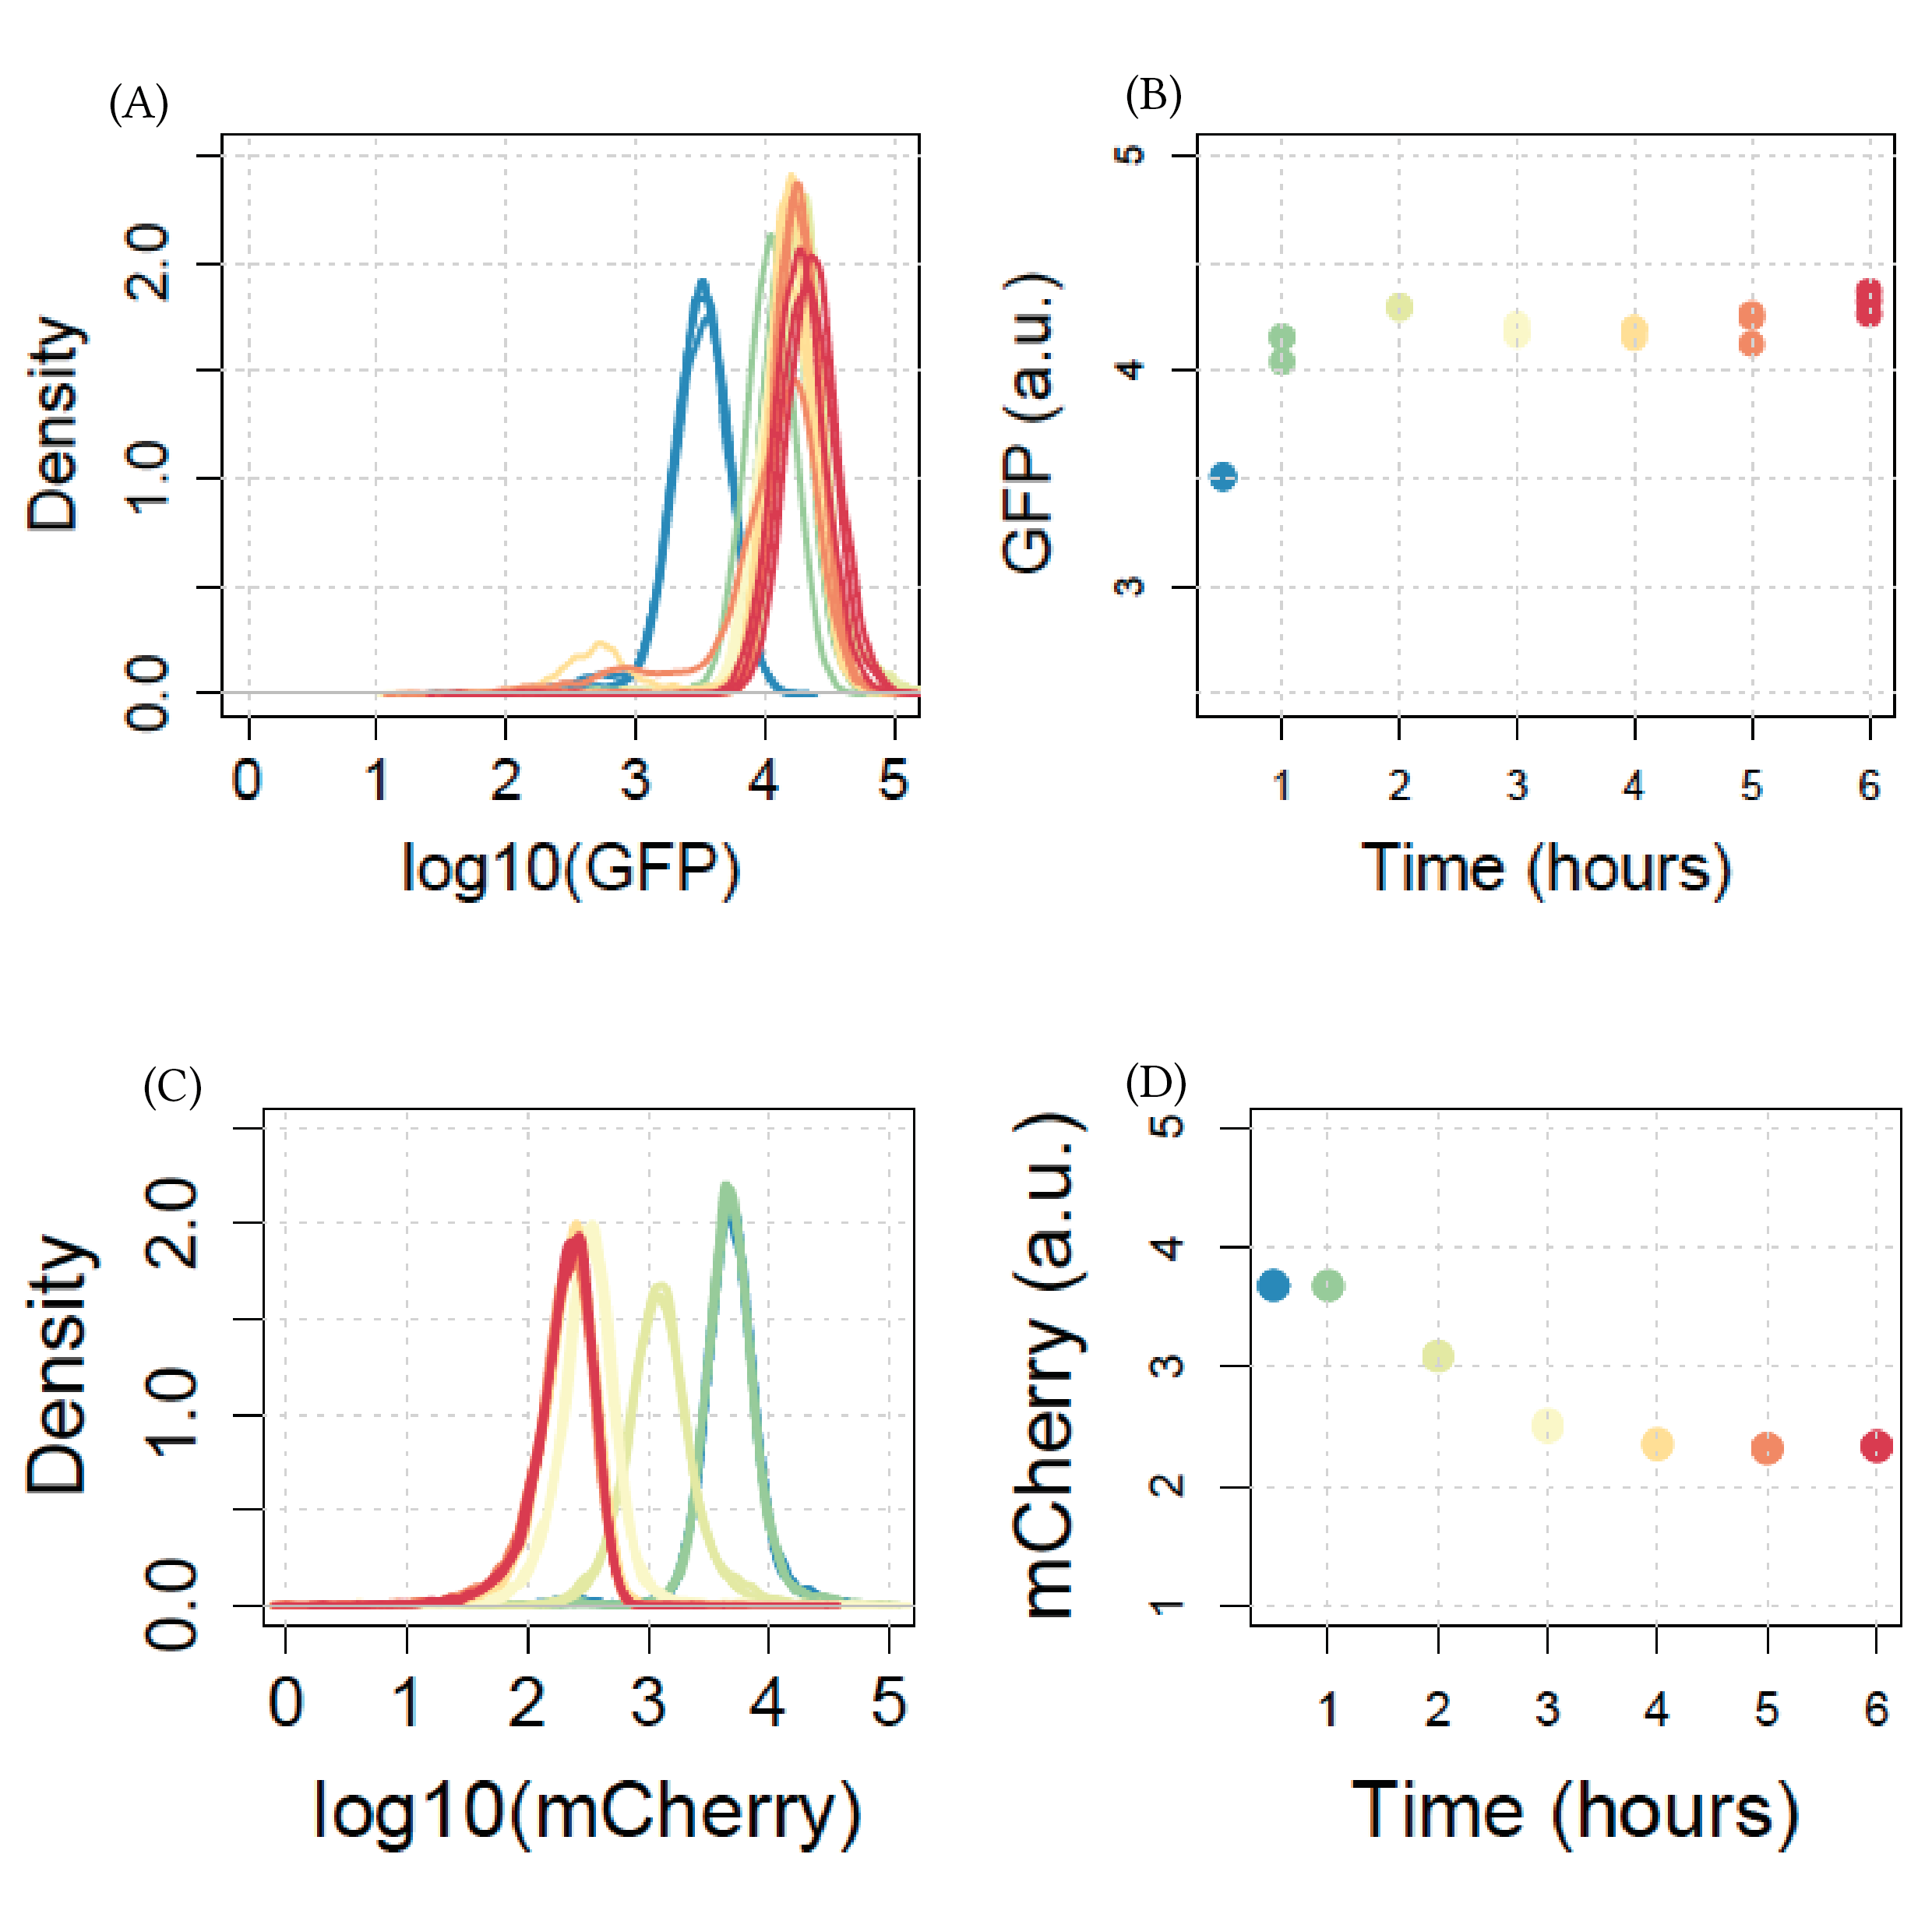
\includegraphics[scale=0.5]{../../chapters/chapterABCFlow/images/atc_timecourse.png}
%\caption[LoF caption]{\label{fig:atc_timecourse}: \acrshort{atc} induction of pKDL071 over time}
%\end{center}
%\end{figure*}
%
%\begin{figure*}[tb]
%	\begin{center}
%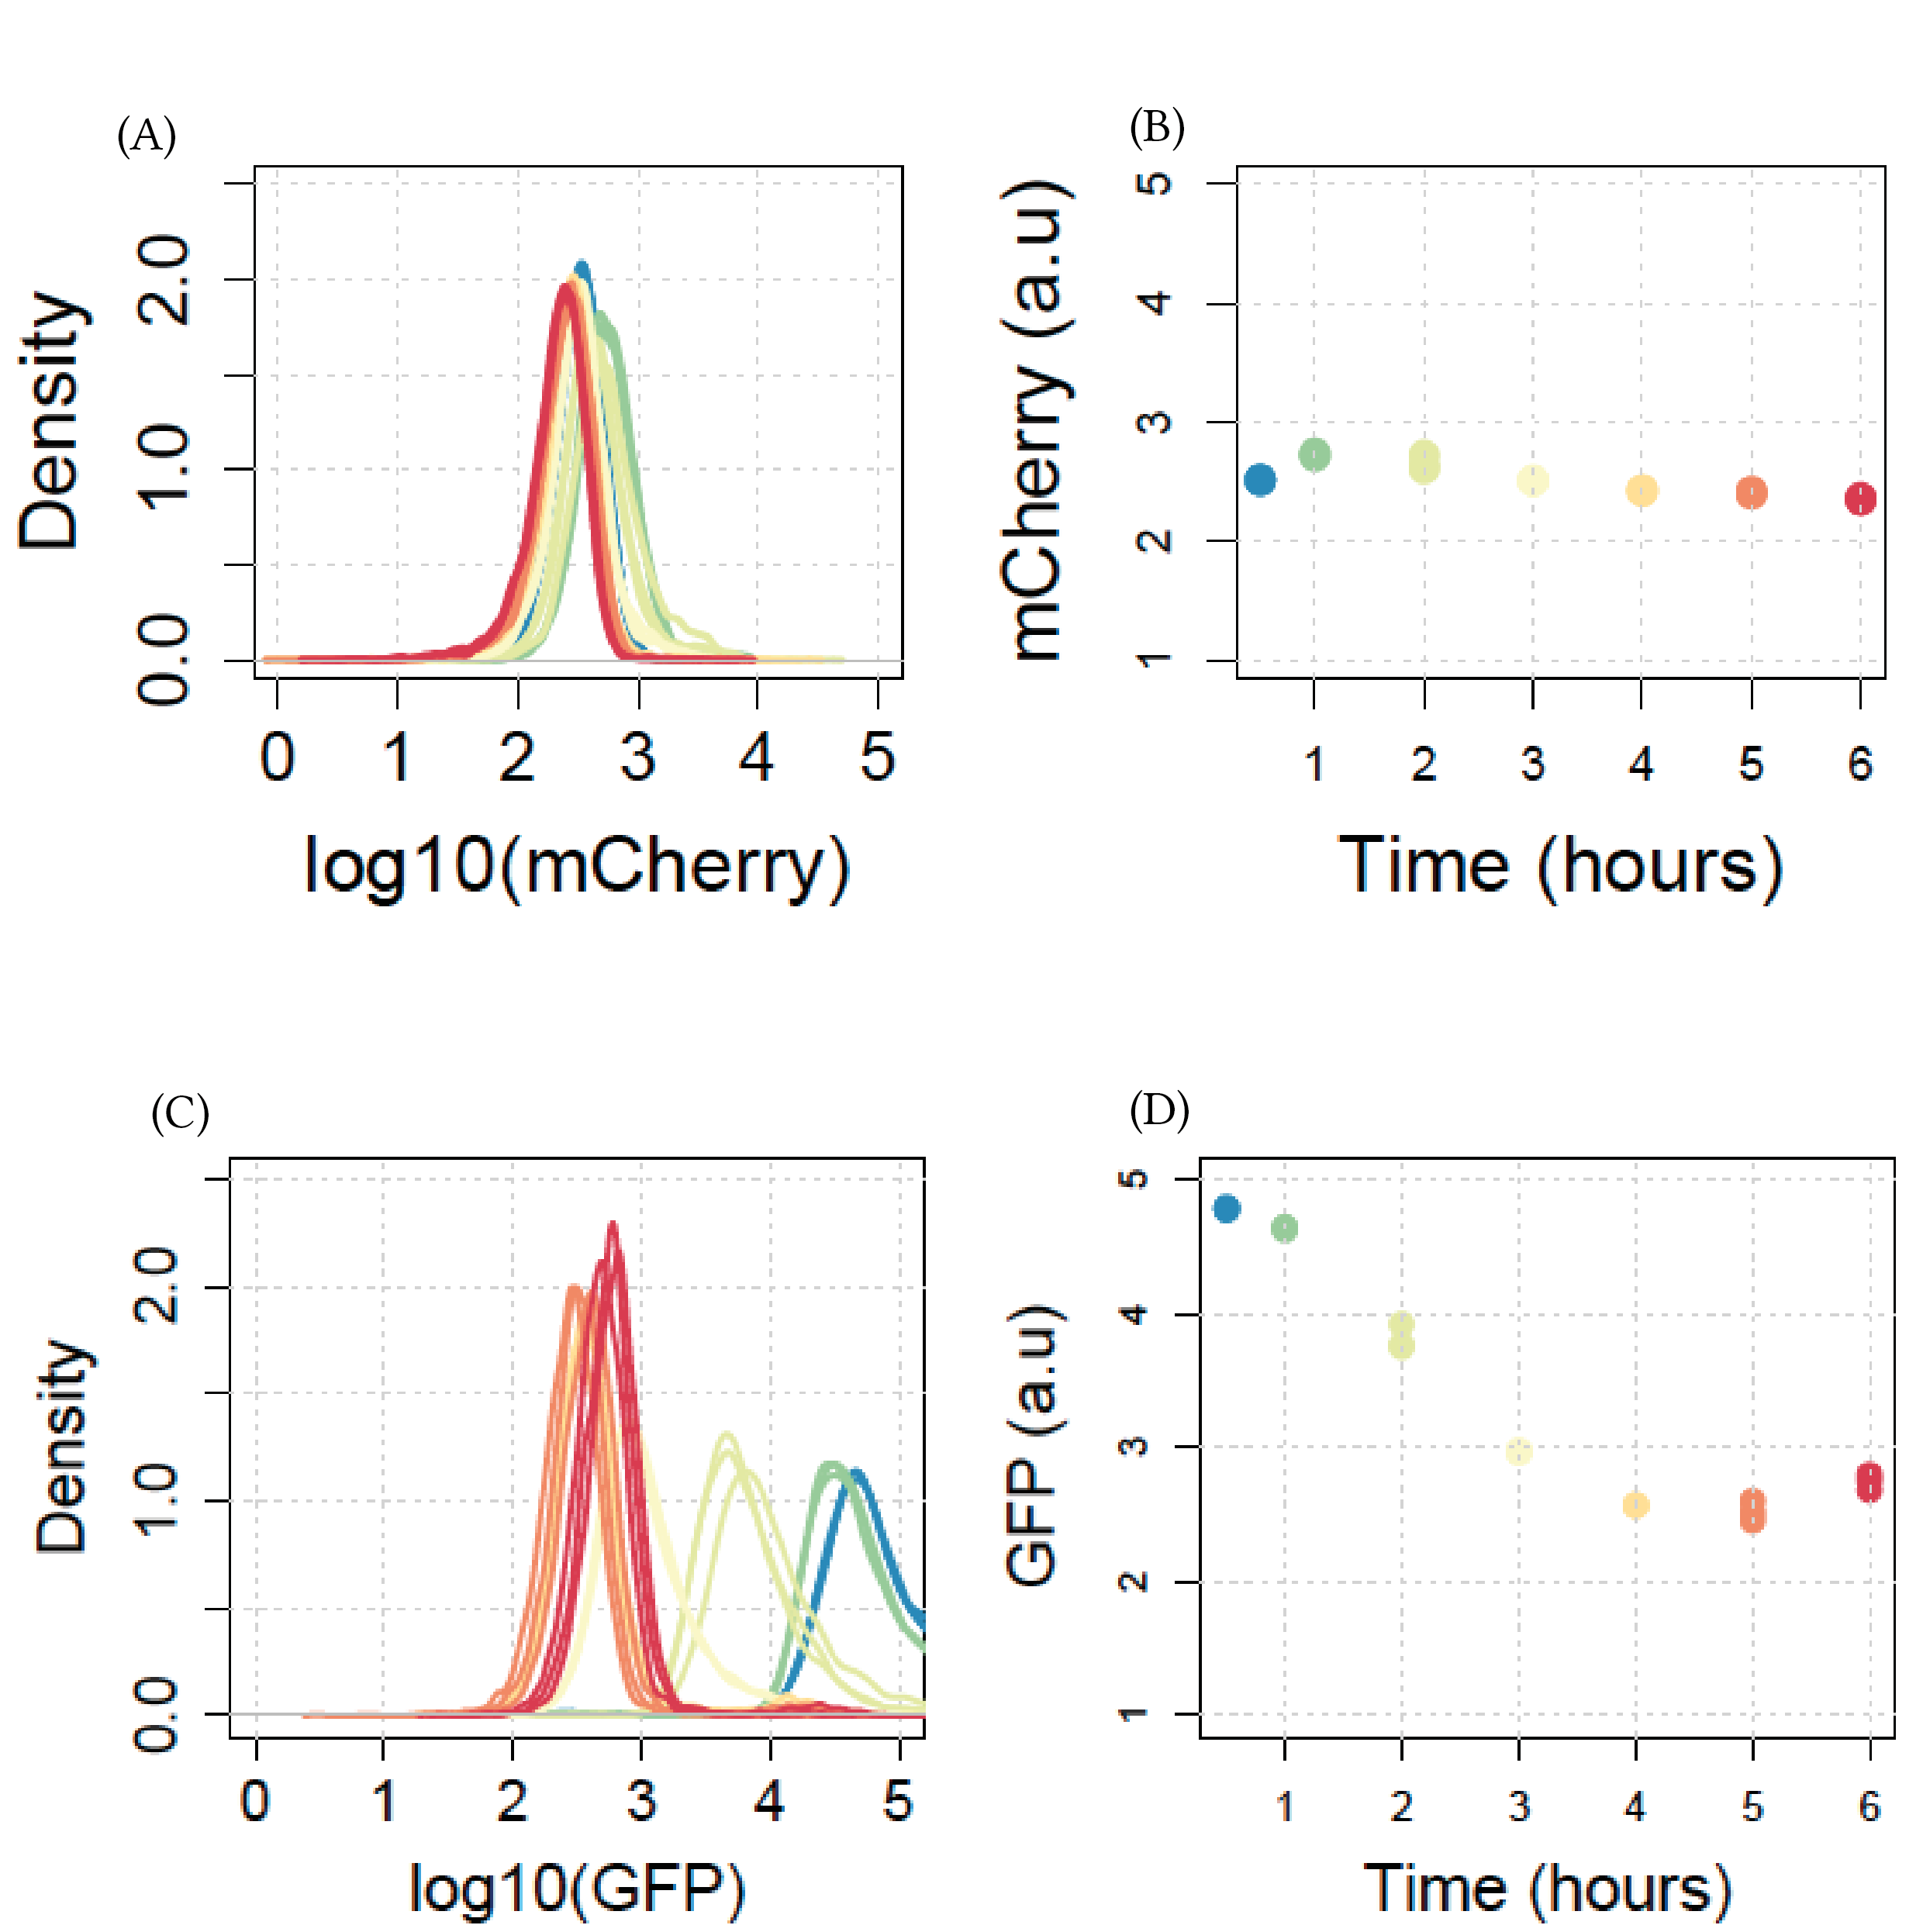
\includegraphics[scale=0.5]{../../chapters/chapterABCFlow/images/iptg_timcourse.png}
%\caption[LoF caption]{\label{fig:iptg_timecourse}: \acrshort{iptg} induction of pKDL071 over time}
%\end{center}
%\end{figure*}
%\clearpage

\section{ABC-Flow parameter inference for experimental data}
 
In this section I apply ABC-Flow to the experimental flow cytometry data collected in Section~\ref{sec:ts_time}. The data set is comprised of time course data of the~\textcite{Litcofsky:2012gr} toggle switch. The two states of the switch are represented by the levels of GFP and mCherry intensity in each bacterial cell. Using \acrshort{atc} inducer, each cell transitions from a GFP low/mCherry high state to a GFP high/mCherry low state and using \acrshort{iptg} each cell transitions from a GFP high/mCherry low state to an GFP high/mCherry high state. 


\subsection{Toggle switch model developed to fit to flow cytometry data}
\label{sec:Real_model}
The model used to fit the toggle switch time course assays was developed by using the Shea-Ackers formalism which represents the probability of a given promoter expressing~\autocite{Ackers:1982tq}, as shown in Figure~\ref{fig:shea-flow}. The Shea-Ackers formalism is described in Section~\ref{sec:shea-ackers}. The model represents the two promoters, P\textsubscript{trc2} and P\textsubscript{Ltet-O} expressing mCherry and GFP respectively. The switch present in plasmid pKDL071 has been simplified to only take into account the two genes GFP and mCherry and it does not include LacI and TetR. Therefore in the model GFP represses the expression of mCherry and vice versa. 


\begin{figure}[tb]
\centerfloat
	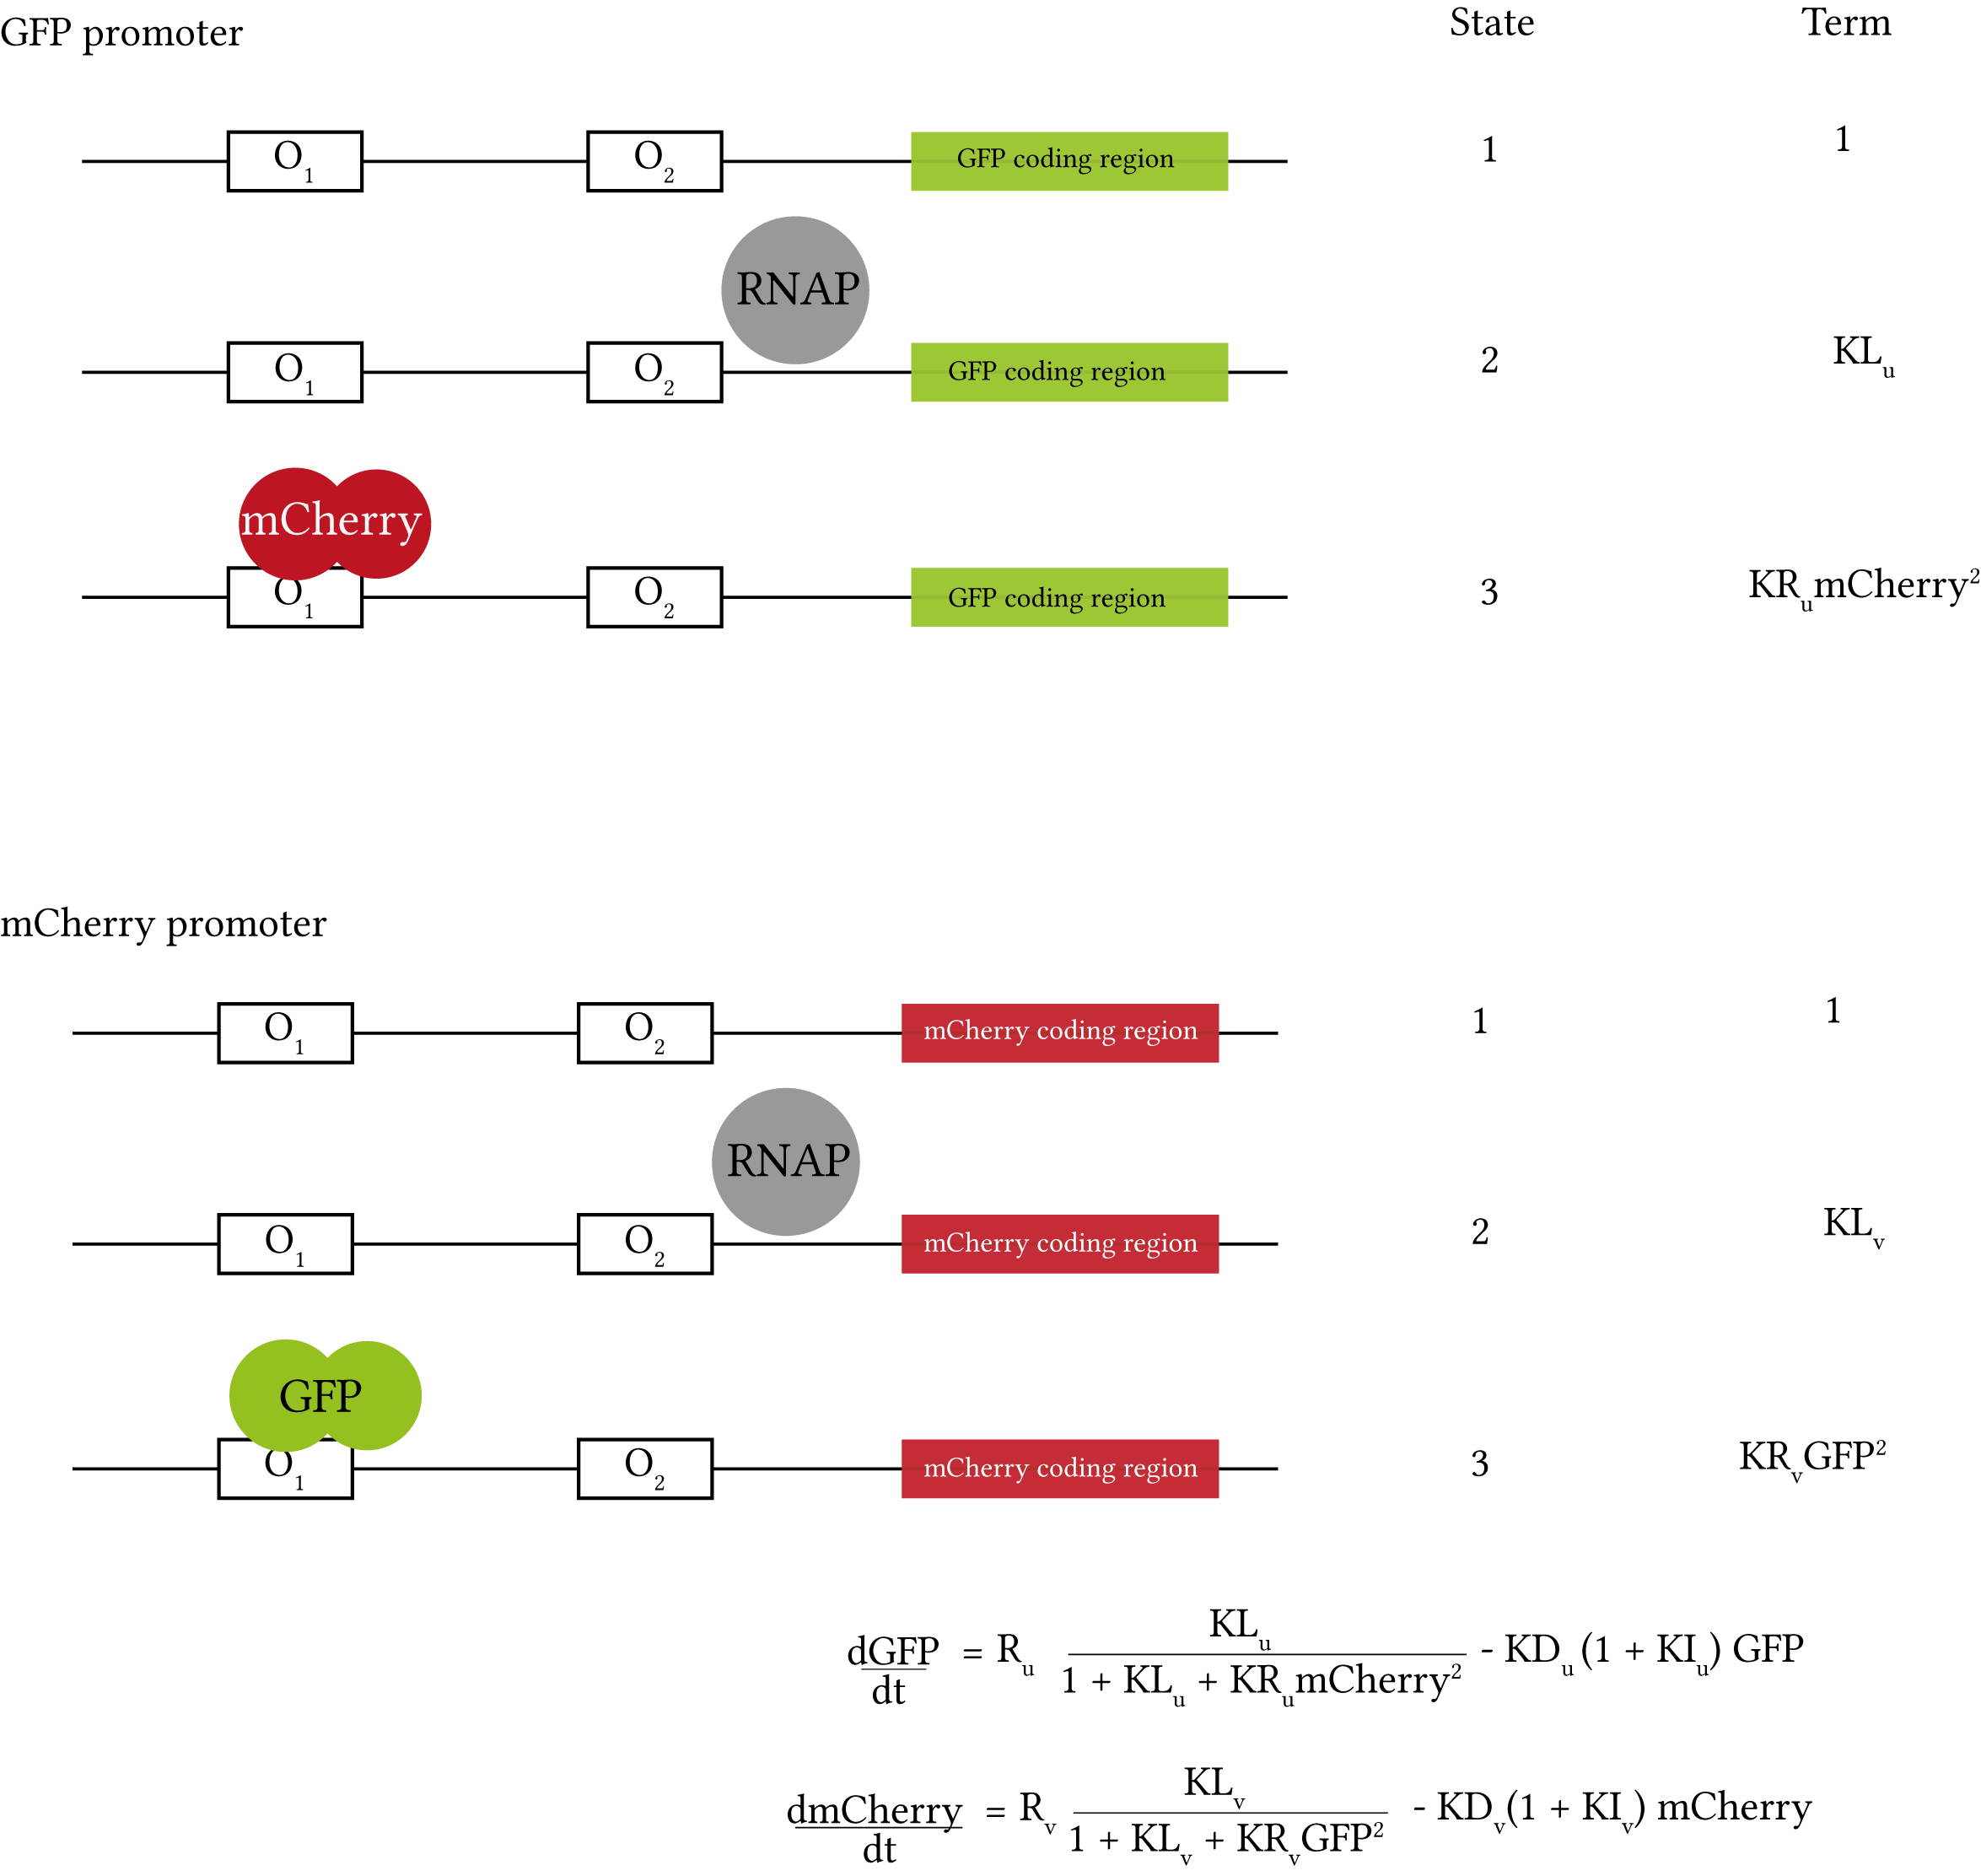
\includegraphics[width=\textwidth]{../../chapters/chapterABCFlow/images/shea-ackers_flow.png}
	\caption[pKDL071 switch model using the Shea-Ackers formalism]{\label{fig:shea-flow}pKDL071 switch model using the Shea-Ackers formalism}
\end{figure}



In order to take into account the stochastic dynamics of the system, the Gillespie algorithm is used in ABC-Flow, and thus the toggle switch model is described by the following hazards:

\begin{align}
h_1 &= KD_u  (1 + KI_u)  GFP\\
h_2 &= 60  \frac{R_u KL_u}{1 + KL_u + KR_u  mCherry^2}\\
h_3 &= KD_v  (1 + KI_v)  mCherry\\
h_4 &= 60  \frac{R_v  KL_v}{1+ KL_v + KR_v  GFP^2},
\end{align}    
     %KI\textsubscript{u} and KI\textsubscript{v} KL\textsubscript{u} KL\textsubscript{v} KD\textsubscript{u} KD\textsubscript{v} KR\textsubscript{u} KR\textsubscript{v},
\noindent where GFP and mCherry represent the two fluorescent proteins in the system. The cooperativity of the repressors (GFP and mCherry) is assumed in the model as well as the dimerization of the inducers. Parameters KI\textsubscript{u} and KI\textsubscript{v} increase the degradation of one of the species, and simulates the addition of a repressor, IPTG or \acrshort{atc} respectively. When using this model to fit to the post-\acrshort{atc} induction time course data, KI\textsubscript{v} was set to 0. KI\textsubscript{u} was set to 0, until t = 0.01h where the prior distribution was used. This was done to simulate the addition of the inducer. When using this model to fit the post-IPTG induction time course, KI\textsubscript{u} was set to 0 and KI\textsubscript{v} sampled from the prior after t = 0.01h. 

The two production hazards, $h2$ and $h4$ are multiplied by 60 to reflect the copy number of the toggle switch plasmid in each cell. The plasmid containing the toggle switch used here, pKDL071, contains the ColE1 origin of replication, and thus 50-70 copies of the plasmid are present in each cell~\autocite{Milo:2010cz}. The priors used in ABC-Flow for this model are given in Table~\ref{tab:priors_model_real}. All priors given assume a uniform distribution. The values of the prior were chosen in agreement with~\autocite{Lillacci:2013hu} and in reference to \url{http://bionumbers.hms.harvard.edu/}, the database of useful biological numbers~\autocite{Milo:2010cz}. 

The model also included a fluorescence intensity part. The fluorescent signal emitted by each individual fluorescent molecule was assumed to be normally distributed around a mean μ and standard deviation σ, as defined in Equation~\ref{eq:intens}. In order to account for background fluorescence I used the OFF state of each side of the switch. Overnight inductions of the plasmid pKDL071, with \acrshort{atc} or IPTG, resulted in the switch fully flipped to each state mCherry low/GFP high and mCherry high respectively. The fluorescent levels of the fluorescent proteins in the low state were assumed to be the background fluorescence detected by the flow cytometer. This was assumed to be a sample from a normal distribution with μ = 100 and σ\textsuperscript{2} = 50 that was added to the signal at each time point. The populations were allowed to progress until the reduction in epsilon started to plateau and the acceptance rate became very low. This indicates that the fit will not improve significantly with subsequent populations.


%The final epsilon used in both switch inductions was set to 10. This is a sufficient distance in order to obtain a distribution that is close to the experimental data set, as shown in Section~\ref{sec:dist}. Nevertheless, given that the data set does not represent a normal distribution, it was not possible to obtain a fit with such a low epsilon value. 


\begin{table}[htbp]
\centering
\caption{The priors used for the 1D and 2D ABC-Flow model fitting to flow cytometry data}
\label{tab:priors_model_real}
\rotatebox{90}{
\begin{tabular}{@{}lllll@{}}
\toprule
\multicolumn{5}{c}{Parameters} \\ \midrule
\multicolumn{1}{c}{Description} & \multicolumn{1}{c}{Symbol} & Units & \multicolumn{1}{c}{\acrshort{atc} induction} & IPTG induction \\ \midrule
IPTG-induced mCherry degradation rate & KI\textsubscript{u} &  h\textsuperscript{−1} μM\textsuperscript{−1}&  & 1 - 100 \\
GFP transcription rate & R\textsubscript{u} & molecules h\textsuperscript{−1} & 1 - 50 & 1 - 50 \\
GFP translation rate & KL\textsubscript{u} & h\textsuperscript{−1} & 1 - 50 & 1 - 50 \\
GFP degradation & KD\textsubscript{u} & h\textsuperscript{−1} & 0.001 - 0.1 & 0.001 - 0.1 \\
mCherry-induced GFP repression rate & KR\textsubscript{u} &  molecules\textsuperscript{−1} h\textsuperscript{−1} & 0.016 - 1.2 & 0.016 - 1.2 \\
mCherry transcription rate & R\textsubscript{v} & molecules h\textsuperscript{−1} & 1 - 50 & 1 - 50 \\
mCherry translation rate & KL\textsubscript{v} & h\textsuperscript{−1} & 1 - 50 & 1 - 50 \\
GFP-induced mCherry repression rate & KR\textsubscript{v} & molecules\textsuperscript{−1} h\textsuperscript{−1} & 0.016 - 1.2 & 0.016 - 1.2 \\
mCherry degradation & KD\textsubscript{v} & h\textsuperscript{−1} & 0.1 - 2 & 0.1 - 2 \\
\acrshort{atc}-induced GFP degradation rate & KI\textsubscript{v} & h\textsuperscript{−1} μM\textsuperscript{−1} & 1 - 100 &  \\ \midrule
\multicolumn{5}{c}{Species} \\ \midrule
 & GFP & mM & 0 - 1 & 100 - 1000 \\
 & mCherry & mM & 100 - 1000 & 0 - 1 \\ \midrule
\multicolumn{5}{c}{Intensity parameters} \\ \midrule
Mean of fluorescence of single GFP molecule & μ\textsubscript{GFP} & AU & 5 - 200 & 5 - 200 \\
Mean of fluorescence of single mCherry molecule & μ\textsubscript{mCherry} & AU & 5 - 200 & 5 - 200 \\
Standard deviation of fluorescence of single GFP molecule & σ\textsubscript{GFP} & AU & 5 - 200 & 5 - 200 \\
Standard deviation of fluorescence of single mCherry molecule & σ\textsubscript{mCherry} & AU & 5 - 200 & 5 - 200 \\ \bottomrule
\end{tabular}
}
\end{table}
\clearpage



\subsection{Model fitting to the genetic toggle switch post \acrshort{atc} induction}

The priors shown in Table~\ref{tab:priors_model_real}, the hazard functions defining the model and the flow cytometry time course data were also supplied to ABC-Flow. ABC-Flow was used to infer the parameter values that could produce the best fit to the experimental data. The resulting simulated time course data and posterior distributions are given in Figures~\ref{fig:1d-real-res} and~\ref{fig:1atc-post} respectively. The model was also simulated stochastically without converting the number of molecules to fluorescence intensity in order to confirm that the model behaves like a switch. This is shown in Figure~\ref{fig:1d-real-res}B. Following \acrshort{atc} induction, the number of GFP molecules increases and the number of mCherry molecules decreases. 


\begin{figure}[tb]
\centerfloat
	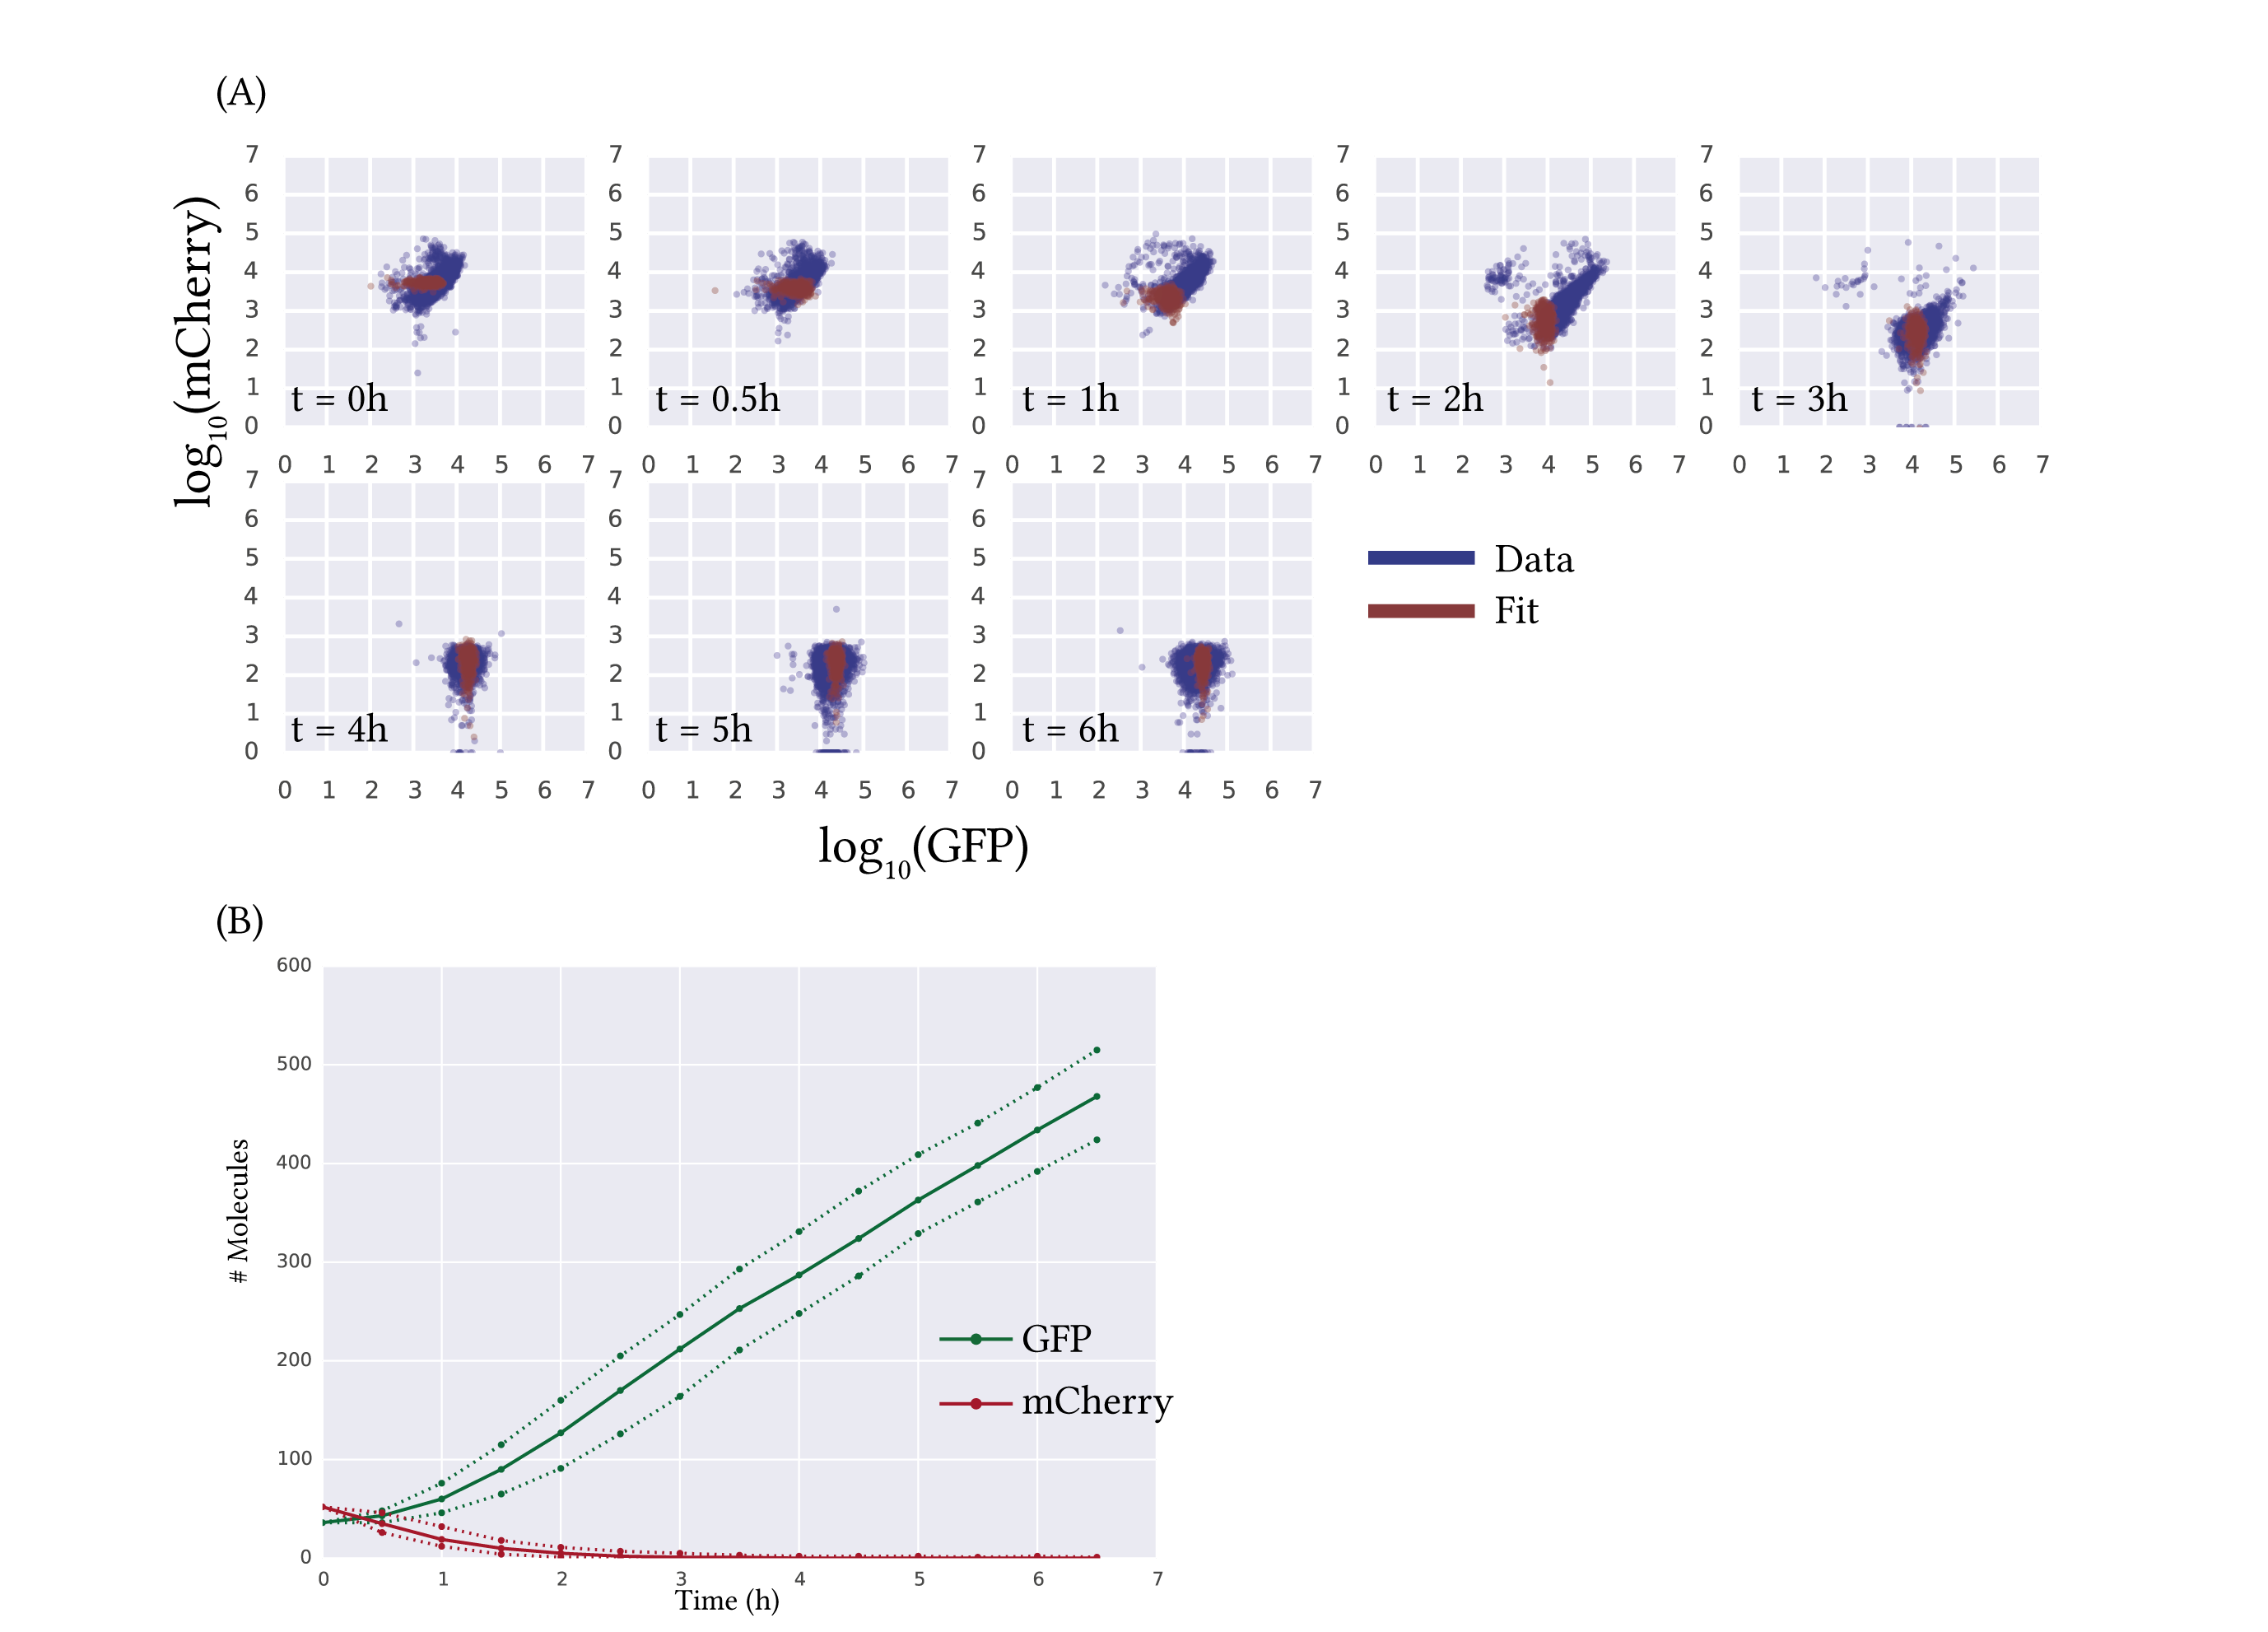
\includegraphics[width=1.2\textwidth]{../../chapters/chapterABCFlow/images/2D_real_res.png}
	\caption[ABC-Flow fit to post-\acrshort{atc} time course data]{\label{fig:1d-real-res} (A) The post-\acrshort{atc} induction flow cytometry time course data (blue) and the resulting model fit from ABC-Flow (red). (B) The model simulation using parameters sampled from the posterior distribution shows that this model has a high and low state for GFP. A solid line depicts the median value of the trajectories and the dotted line depict 0.025 and 0.975 quartiles. (C) The particle acceptance rate from ABC-Flow (D) The progression of epsilon threshold values at each population.}
\end{figure}



\begin{figure}[tb]
\centerfloat
	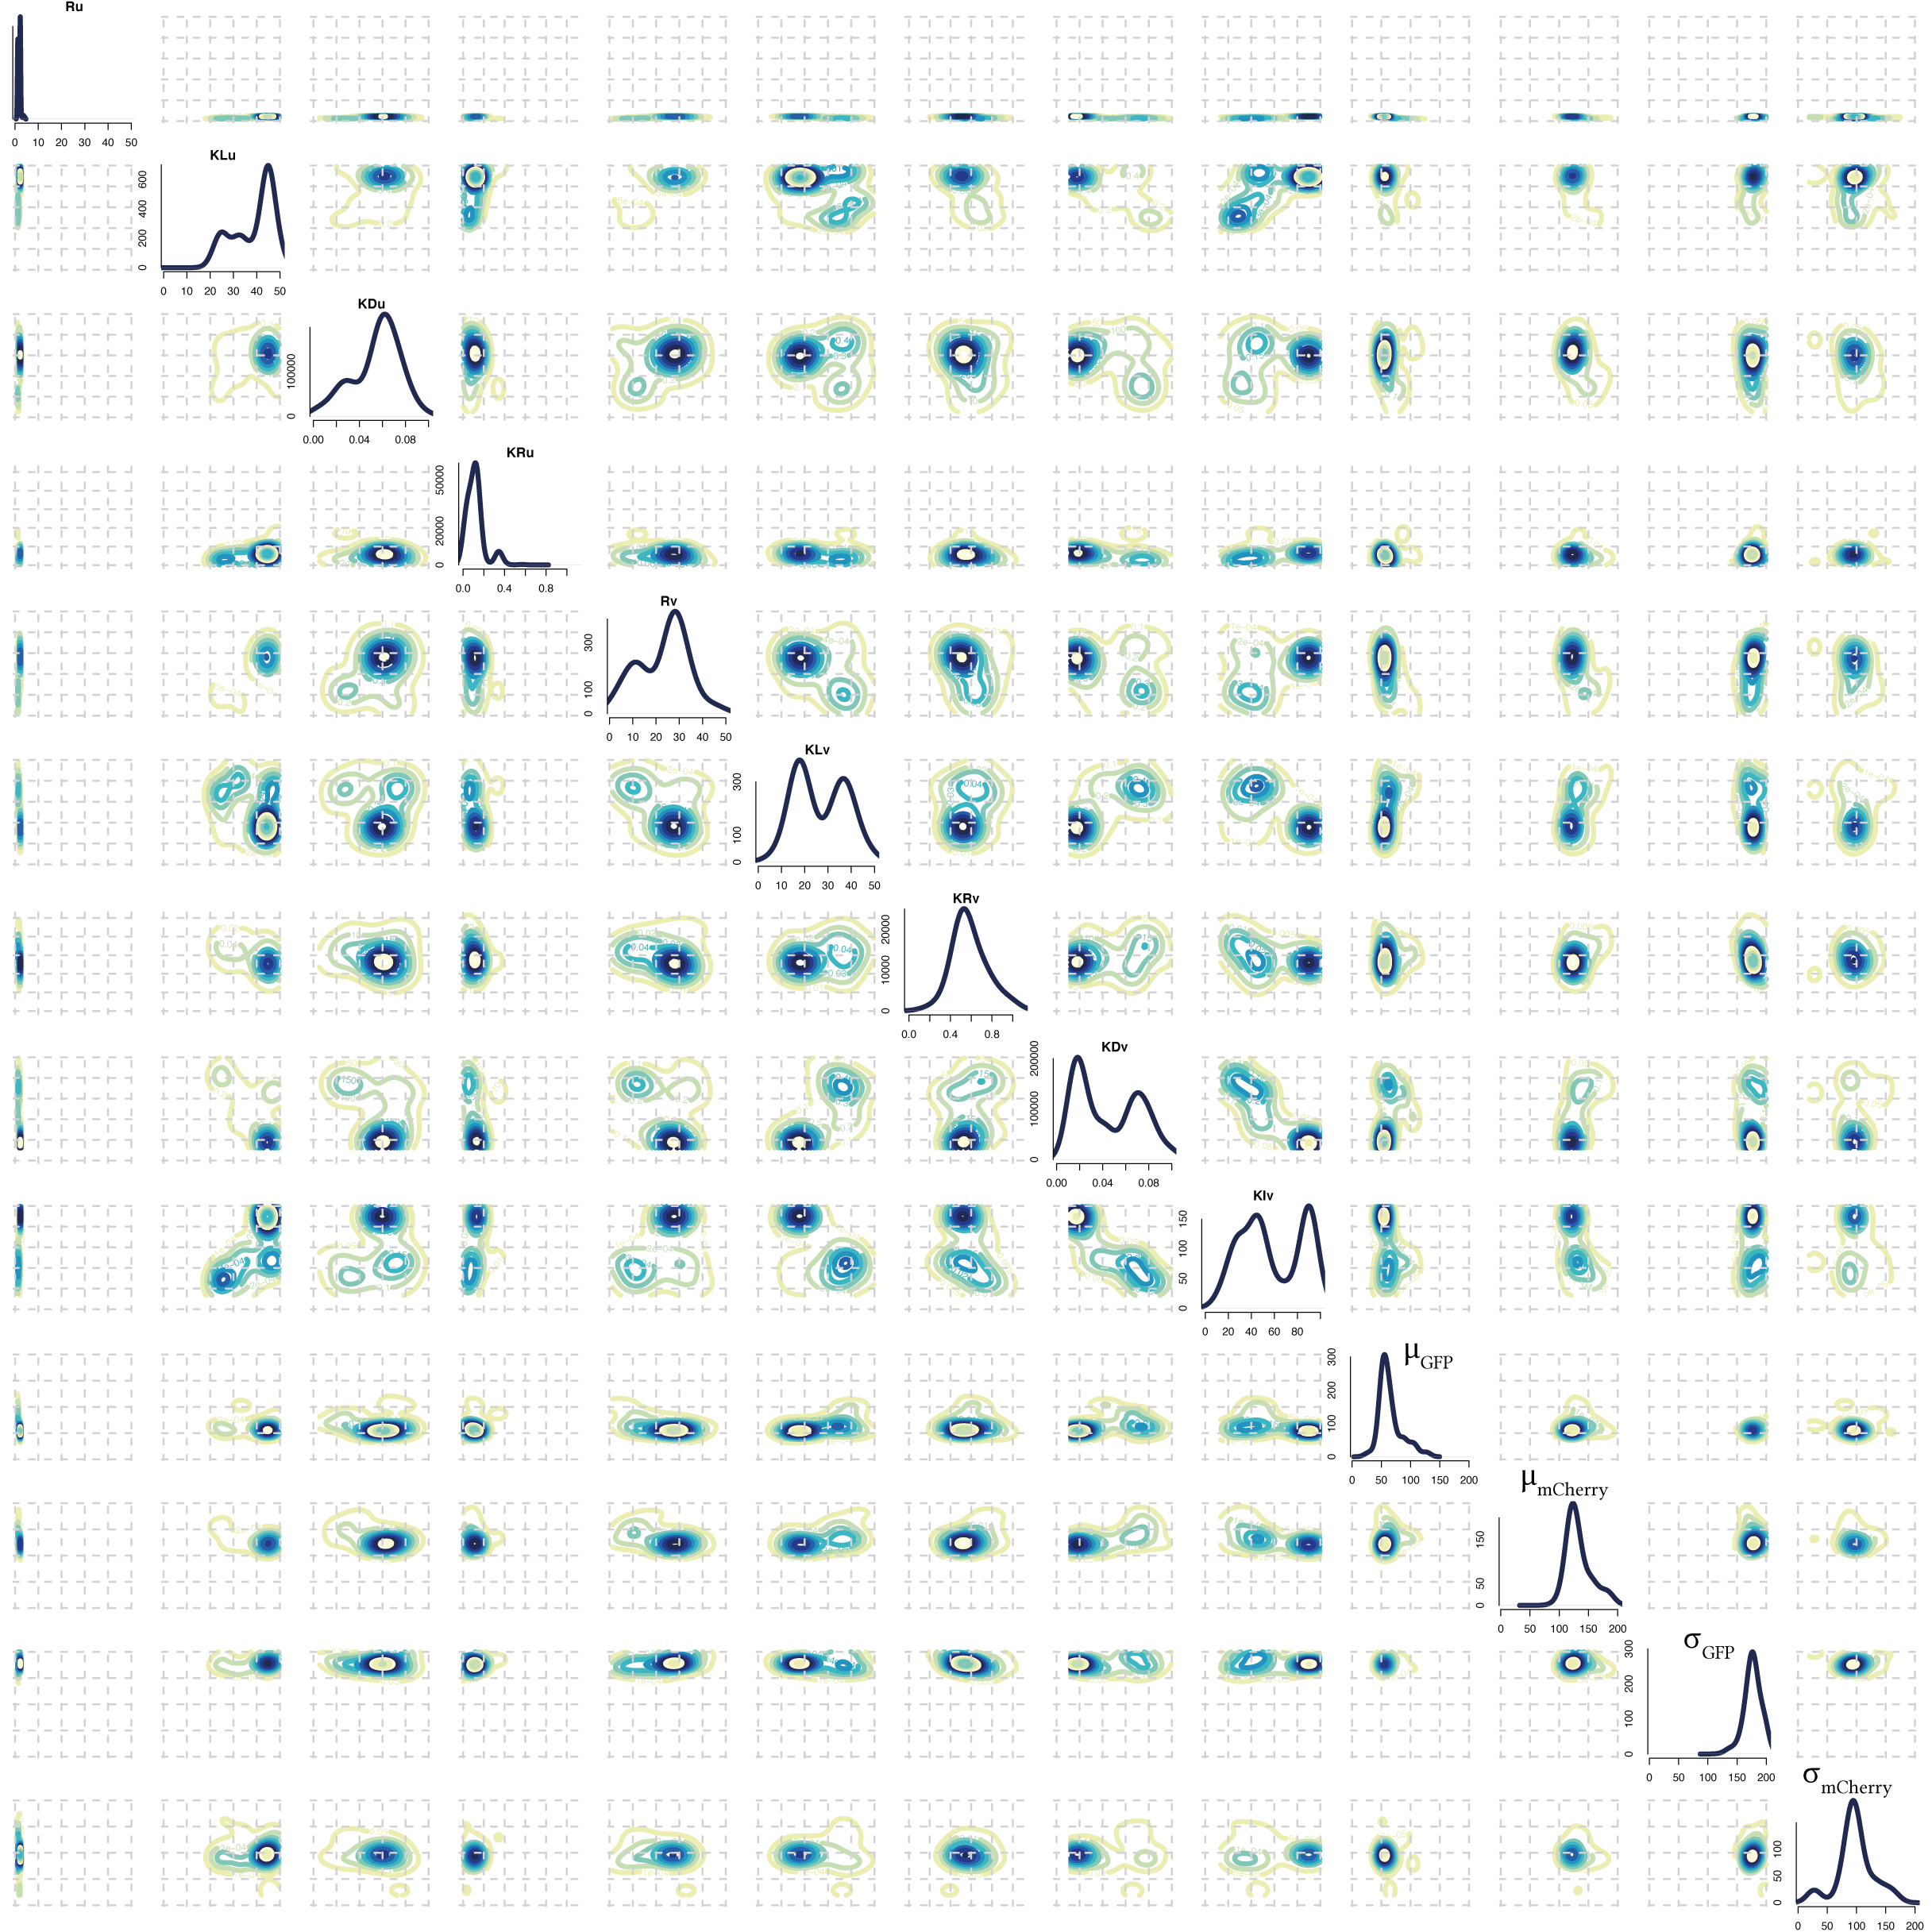
\includegraphics[width=1.1\textwidth]{../../chapters/chapterABCFlow/images/posterior_atc.png}
	\caption[Posterior distribution of inferred parameters for post-\acrshort{atc} induction of the toggle switch]{\label{fig:1atc-post} The posterior distributions of the 13 parameters fitted to post-\acrshort{atc} induction time course data using ABC-Flow. We find that the parameters for GFP expression (R\textsubscript{u}) and repression (KR\textsubscript{u}) are the most identifiable.}
\end{figure}



% The parameter for the repression of GFP by mCherry (KR\textsubscript{u}) was inferred to be () . The median values of all inferred parameters, with the 95\% confidence intervals, are given in Table~\ref{tab:inf_params_atc}. 

The inferred parameters, and the 95\% credible intervals, are given in Table~\ref{tab:inf_params_atc}. In order to validate these results I compare the 95\% confidence intervals of the inferred parameters to values reported in the literature. First the half-lives of the two proteins in the system, GFP and mCherry are estimated. The half-life of a protein is given by 

\begin{align*}
	t_{\frac{1}{2}} = \frac{ln(2)}{k}
\end{align*}

\noindent where $k$ is the decay rate of the protein. The half-life of GFP was estimated to be (7.788, 43.322) hours which is consistent with the \textgreater 24 hours half life that has been previously reported for the variant of GFP used here, GFPmut3b~\autocite{Andersen:1998tn}. The half-life for mCherry was estimated to be (9.242, 31.507) hours which is consistent with the long half-life of mCherry, reported to be more than 24 hours~\autocite{Shaner:2004vy}. We find that the inferred parameter for GFP gene expression, R\textsubscript{u} is (1.055, 1.979) molecules h\textsuperscript{-1}, whereas the parameter for gene expression of mCherry (R\textsubscript{v}) was inferred to (8.970, 42.611) molecules h\textsuperscript{-1}. These values correspond to the promoter strengths of P\textsubscript{LtetO-1} and P\textsubscript{trc2} respectively. This is in agreement with characterisation data on the strength of these two promoters, which report that there is a difference in strengths, P\textsubscript{trc2} being a stronger promoter than P\textsubscript{LtetO-1}~\autocite{Litcofsky:2012gr}. Further, we find that the values of the intensity parameters μ and σ, which represent the settings on the flow cytometer, to be inferred better for GFP than for mCherry. 


 %There is an indication of the difference in strengths in the inferred values here, but the value of R\textsubscript{v} has not been inferred as well as R\textsubscript{u} to draw a strong conclusion.


\begin{table}[htb]
\centering
\caption{The inferred parameter values of the toggle switch post-\acrshort{atc} induction}
\label{tab:inf_params_atc}
\begin{tabular}{@{}lllll@{}}
\toprule
Parameter & Units &0.025 & Median & 0.975 \\ \midrule
R\textsubscript{u} &molecules h\textsuperscript{-1}& 1.055 & 1.298 & 1.979 \\
KL\textsubscript{u} &h\textsuperscript{-1}& 0.022 & 0.043 & 0.075 \\
KI\textsubscript{v} &h\textsuperscript{-1}& 19.606 & 40.466 & 49.138 \\
KD\textsubscript{u} &h\textsuperscript{-1}& 0.022 & 0.043 & 0.075 \\
KI\textsubscript{v} &h\textsuperscript{-1}& 0.016 & 0.0834 & 0.089 \\
KR\textsubscript{u} &molecules h\textsuperscript{-1}& 0.006 & 0.013 & 0.093 \\
R\textsubscript{v} &molecules h\textsuperscript{-1}& 8.970 & 31.057 & 42.611 \\
KL\textsubscript{v} &h\textsuperscript{-1}& 5.807 & 35.396 & 38.333 \\
KR\textsubscript{v} &molecules h\textsuperscript{-1}& 0.095 & 0.386 & 0.947 \\
KD\textsubscript{v} &h\textsuperscript{-1}& 0.022 & 0.043 & 0.075 \\
KI\textsubscript{v} &h\textsuperscript{-1} μM\textsuperscript{-1}& 21.690 & 54.214 & 89.937 \\
μ\textsubscript{GFP} &AU& 53.424 & 76.229 & 84.055 \\
μ\textsubscript{mCherry} &AU& 91.329 & 108.691 & 176.058 \\
σ\textsubscript{GFP} &AU& 154.373 & 193.198 & 196.525 \\
σ\textsubscript{mCherry} &AU& 68.178 & 115.581 & 139.816 \\ \bottomrule
\end{tabular}
\end{table}

The inferred parameters can be used to study the switch system present in the pKDL071 plasmid. Here I examined the effect that the values of the most well inferred parameters, R\textsubscript{u} and KR\textsubscript{u} as well as the initial conditions have on the behaviour of the system. The results are shown in Figure~\ref{fig:prom_str}. First, I studied the effect of the initial conditions of the dominant protein, in this case mCherry has on the system. In order to do that I simulated the model using the median values from the posterior distribution, and increased the initial condition value of mCherry. We do not find this to have had an effect on the final state of the system, as GFP reaches a similar value at 6 hours as the one produced using inferred initial condition values (shown in Figure~\ref{fig:prom_str}B). On the other hand, decreasing the initial condition values of GFP to 10 molecules, destabilises the switch, as shown in Figure~\ref{fig:prom_str}B. The switch happens at a later time point, and it does not take place for all stochastic trajectories.   

The value of R\textsubscript{u} represents the strength of the promoter driving GFP expression. It is therefore important to understand the effect that the promoter strength has on the behaviour of the system. In order to do that, I simulated the model with values that exceed the 95\% credible region of the values inferred from ABC-Flow. The results are shown in Figure~\ref{fig:prom_str}C and D. We find that if the promoter strength is lower than the range of the 95\% credible region of the inferred value then the system stops behaving like a switch. If the value is much higher, GFP reaches a much higher value after 6 hours. Further, I examine the effect that the strength of KR\textsubscript{u}, the parameter representing the mCherry-induced GFP repression rate, has to the behaviour of the system. We find that KR\textsubscript{u} affects the ability of the system to behave like a switch. If KR\textsubscript{u} is set to 0.1, the switch occurs at a later time point, and does not take place for all stochastic trajectories. If KR\textsubscript{u} is set to much higher than the 95\% credible region, the system does not switch. These findings are important in the understanding the system under study as they allow the above predictions to be made about the behaviour of the system.  


\begin{figure}[htb]
\centerfloat
	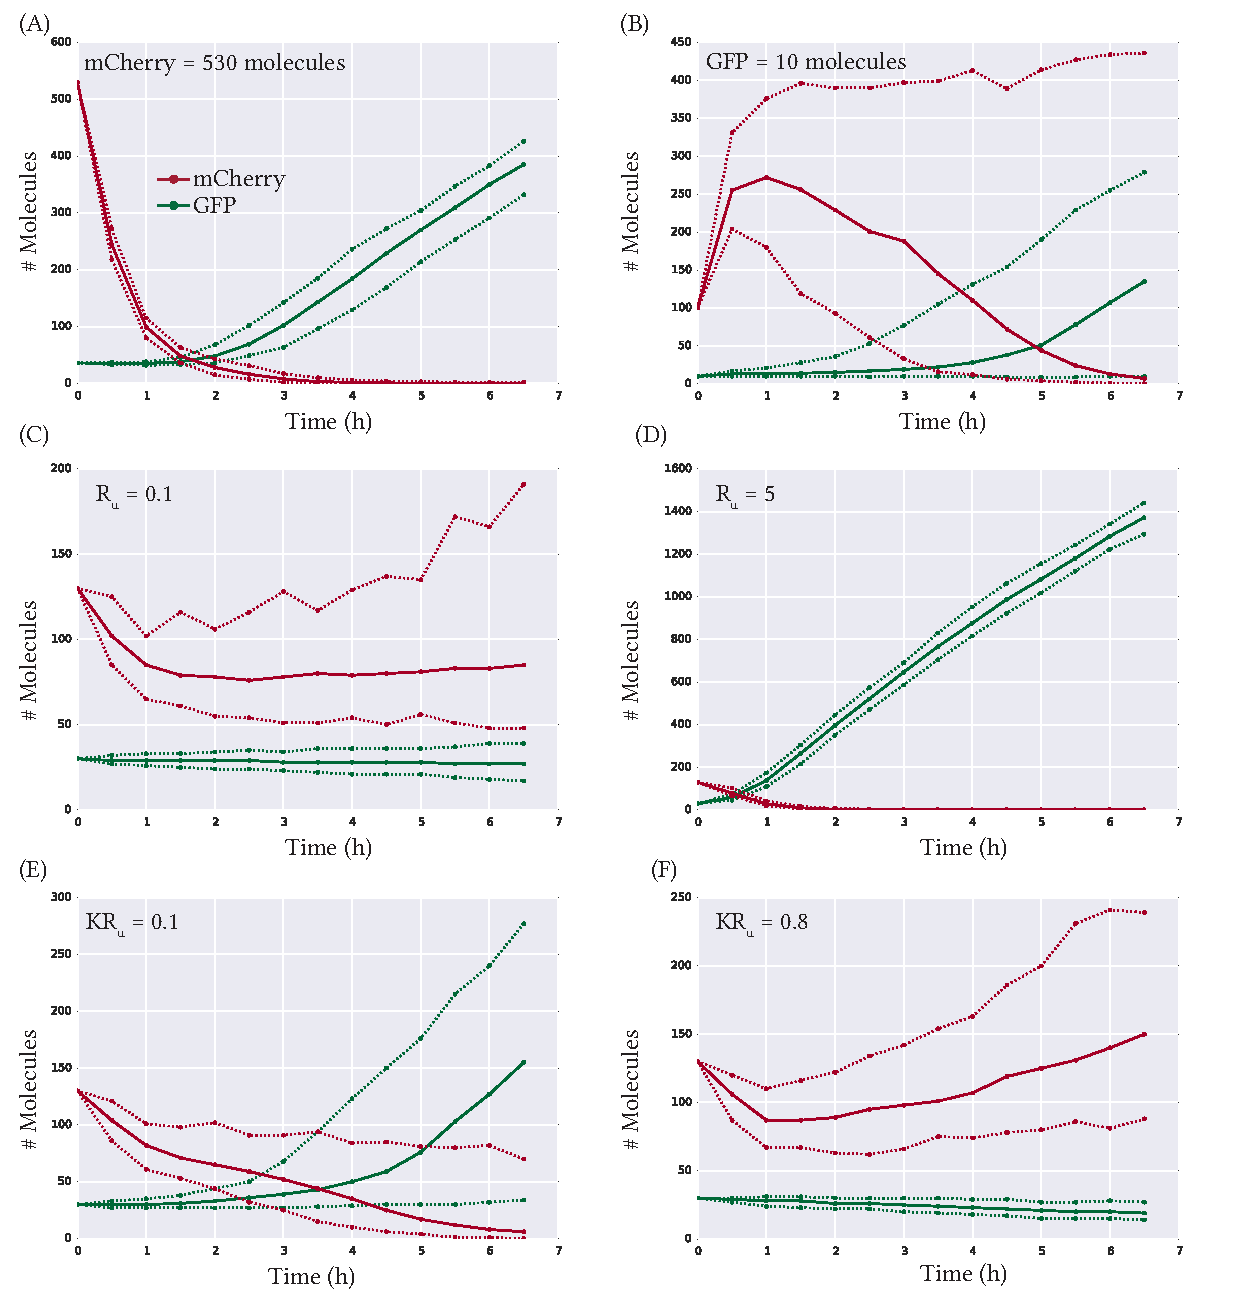
\includegraphics[width=\textwidth]{../../chapters/chapterABCFlow/images/promoter_strengths.pdf}
	\caption[Changing the parameter values affects the behaviour of the switch ]{\label{fig:prom_str} (A) Increasing the initial condition value of mCherry does not affect the state of the system. (B) Decreasing the initial condition value of GFP destabilises the switch. (C) Decreasing parameter R\textsubscript{u} to a value outside the 95\% credible region stops the model from behaving like a switch. (D) Increasing the value of R\textsubscript{u}, the rate representing the transcription factor of GFP, causes GFP to reach higher levels. (E) Increasing  the value of KR\textsubscript{u}, the parameter representing the mCherry-induced GFP repression rate causes the switch to happen at a later time point and not all stochastic trajectories switch state. (F) If the value of KR\textsubscript{u} is set to larger than the 95\% credible region, the system does not switch states. For all plots, a solid line depicts the median value of the trajectories and the dotted line depict 0.025 and 0.975 quartiles.}
\end{figure}



\clearpage
\subsection{Model fitting to the genetic toggle switch post IPTG induction}
ABC-Flow was further used to fit the experimental time course obtained from the toggle switch post-IPTG induction. The prior densities used are given in Table~\ref{tab:priors_model_real}, the hazard functions of the model as well as the flow cytometry data was provided to ABC-Flow. The resulting time course of the model fitted to the experimental flow cytometry data is shown in Figure~\ref{fig:1d-real-res-iptg} and the median and 95\% confidence intervals of the inferred parameters are shown in Table~\ref{tab:inf_params_iptg}.


\begin{figure}[htbp]
\centerfloat%
	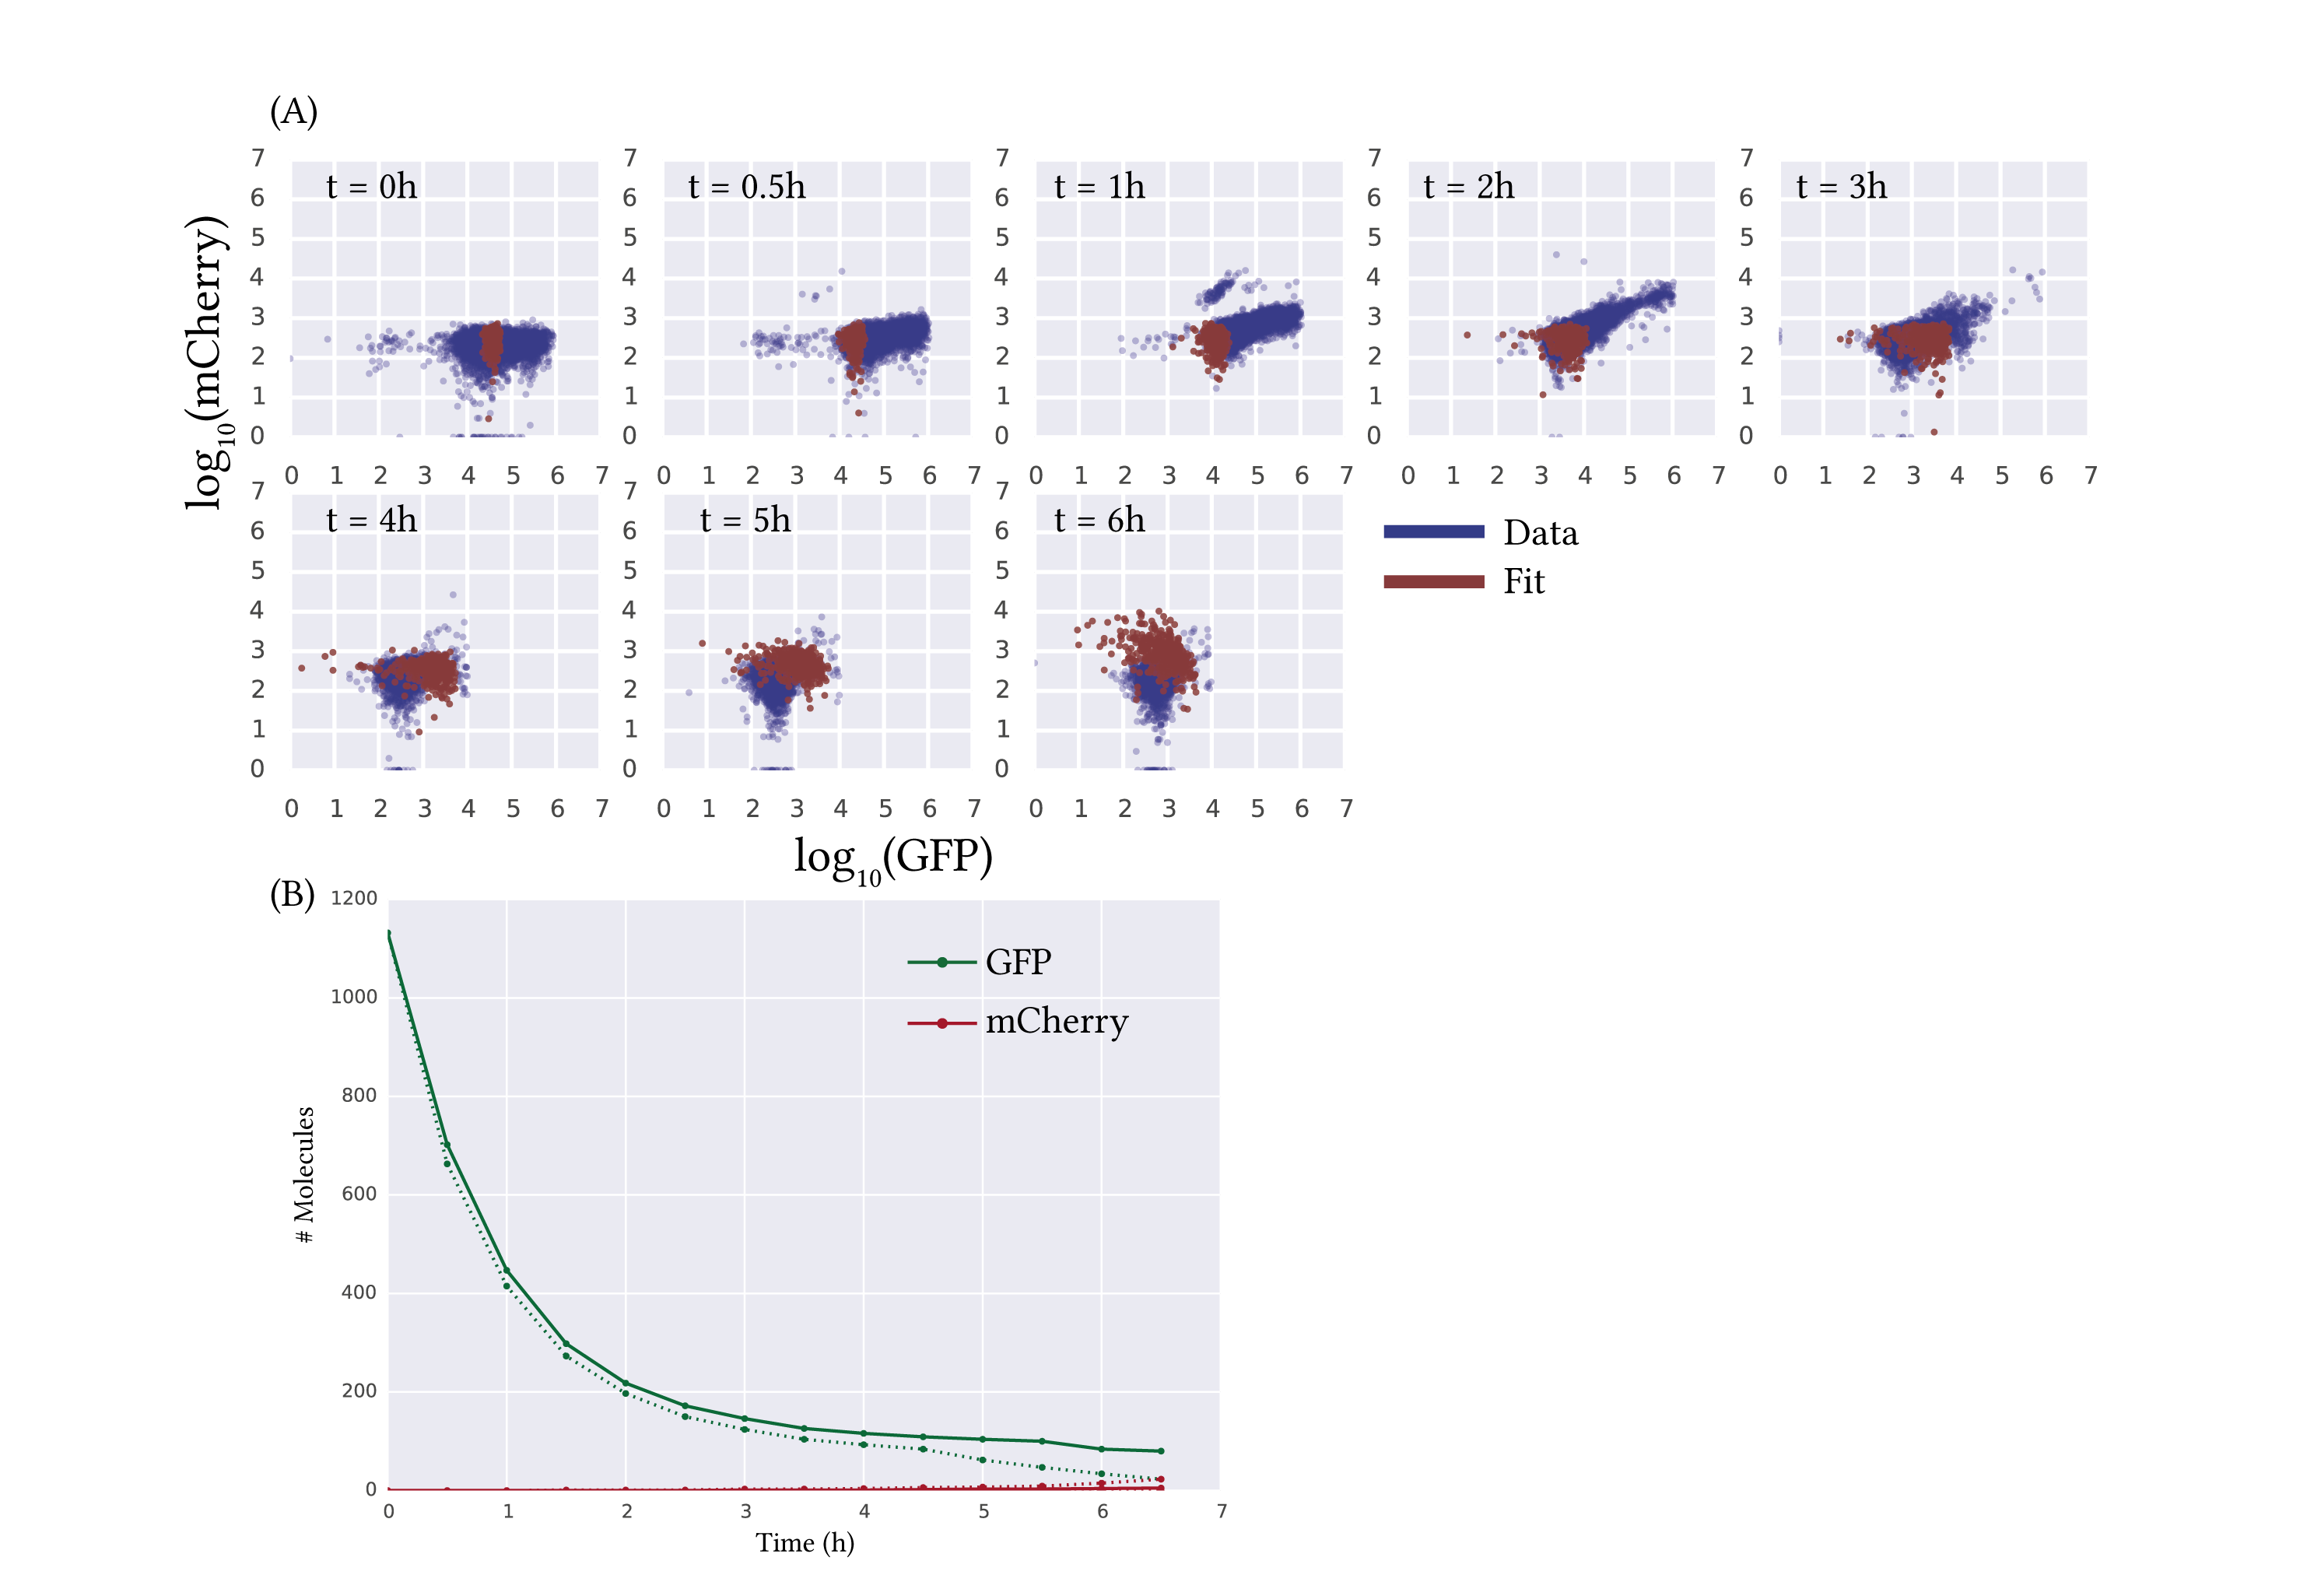
\includegraphics[width=1.2\textwidth]{../../chapters/chapterABCFlow/images/2D_real_res_IPTG.png}
	\caption[ABC-Flow fit to post-\acrshort{atc} time course data]{\label{fig:1d-real-res-iptg} (A) The time course data obtained of the post-IPTG induced toggle switch is shown in blue and the resulting fit from ABC-Flow is shown in red. (B) The model was simulated by using parameter sampled from the posterior distribution. The resulting model did not behave like a switch. (C) The particle acceptance rate from ABC-Flow (D) The progression of epsilon threshold values at each population.  }
\end{figure}

The median values of the marginal posterior distribution of each parameter were used to simulate the model without the conversion to fluorescent intensity in order to confirm that the model behaved like a switch. As can be seen in Figure~\ref{fig:1d-real-res-iptg}B, the model does not behave like a switch within the timeframe given from the experimental data (0 - 6 hours). We find a rapid decay of GFP without an increase in mCherry fluorescence as would be expected. This could be attributed to the experimental time course obtained. As shown in Figure~\ref{fig:1d-real-res-iptg}A, over a period of 6 hours post induction there is a decrease in GFP fluorescence. mCherry can be seen increasing after two hours post induction but then not maintaining that high level. Over the 6 hours, there is no overall increase in mCherry fluorescence. This time course is challenging to fit using the model used here as it does not behave like a switch as expected. The epsilon progression of the fit for the IPTG induction of the switch further confirms that the fit to the data is not as good as expected. Epsilon reduction levels off at a high epsilon value compared to the \acrshort{atc} induction, while the acceptance rate is very low. This indicates that continuing with the fit of the above model to the IPTG induction data will not produce a better fit.   


\begin{table}[tb]
\centering
\caption{The inferred parameter values of the toggle switch post-\acrshort{iptg} induction}
\label{tab:inf_params_iptg}
\begin{tabular}{@{}lllll@{}}
\toprule
Parameter & Units &0.025 & Median & 0.975 \\ \midrule
KI\textsubscript{u} &h\textsuperscript{-1}μM\textsuperscript{-1}& 11.767 & 33.094 & 59.814 \\
R\textsubscript{u} &molecules h\textsuperscript{-1}& 1.057 & 1.818 & 9.707 \\
KL\textsubscript{u} &h\textsuperscript{-1}& 1.161 & 4.986 & 28.258 \\
KD\textsubscript{u} &h\textsuperscript{-1}& 0.015 & 0.031 & 0.083 \\
KR\textsubscript{u} &molecules h\textsuperscript{-1}& 0.146 & 0.839 & 1.183 \\
R\textsubscript{v} &molecules h\textsuperscript{-1}& 1.119 & 3.223 & 21.715 \\
KL\textsubscript{v} &h\textsuperscript{-1}& 1.396 & 11.515 & 33.369 \\
KR\textsubscript{v} &molecules h\textsuperscript{-1}& 0.461 & 0.758 & 1.136 \\
KD\textsubscript{v} &h\textsuperscript{-1}& 0.009 & 0.061 & 0.091 \\
μ\textsubscript{GFP} &AU& 19.371 & 34.634 & 46.499 \\
μ\textsubscript{mCherry} &AU& 17.082 & 34.943 & 138.208\\
σ\textsubscript{GFP} &AU& 151.169 & 179.357 & 197.939 \\
σ\textsubscript{mCherry} &AU& 9.907 & 52.085 & 89.492 \\ \bottomrule
\end{tabular}
\end{table}


The posterior density obtained from by ABC-Flow is given in Figure~\ref{fig:1atc-post}. Parameter R\textsubscript{u}, representing GFP expression, was inferred to be (1.057, 9.707) molecules h\textsubscript{-1}, within the 95\% credible region of the posterior. This is in good agreement with the inferred values obtained for the post-\acrshort{atc} induction. The half-life values obtained for GFP and mCherry were found to be (8.35, 46.20) and (7.61, 77.016) respectively, which are in good agreement with reported literature values~\autocite{Shaner:2004vy, Andersen:1998tn}. 

\begin{figure}[htbp]
\centerfloat
	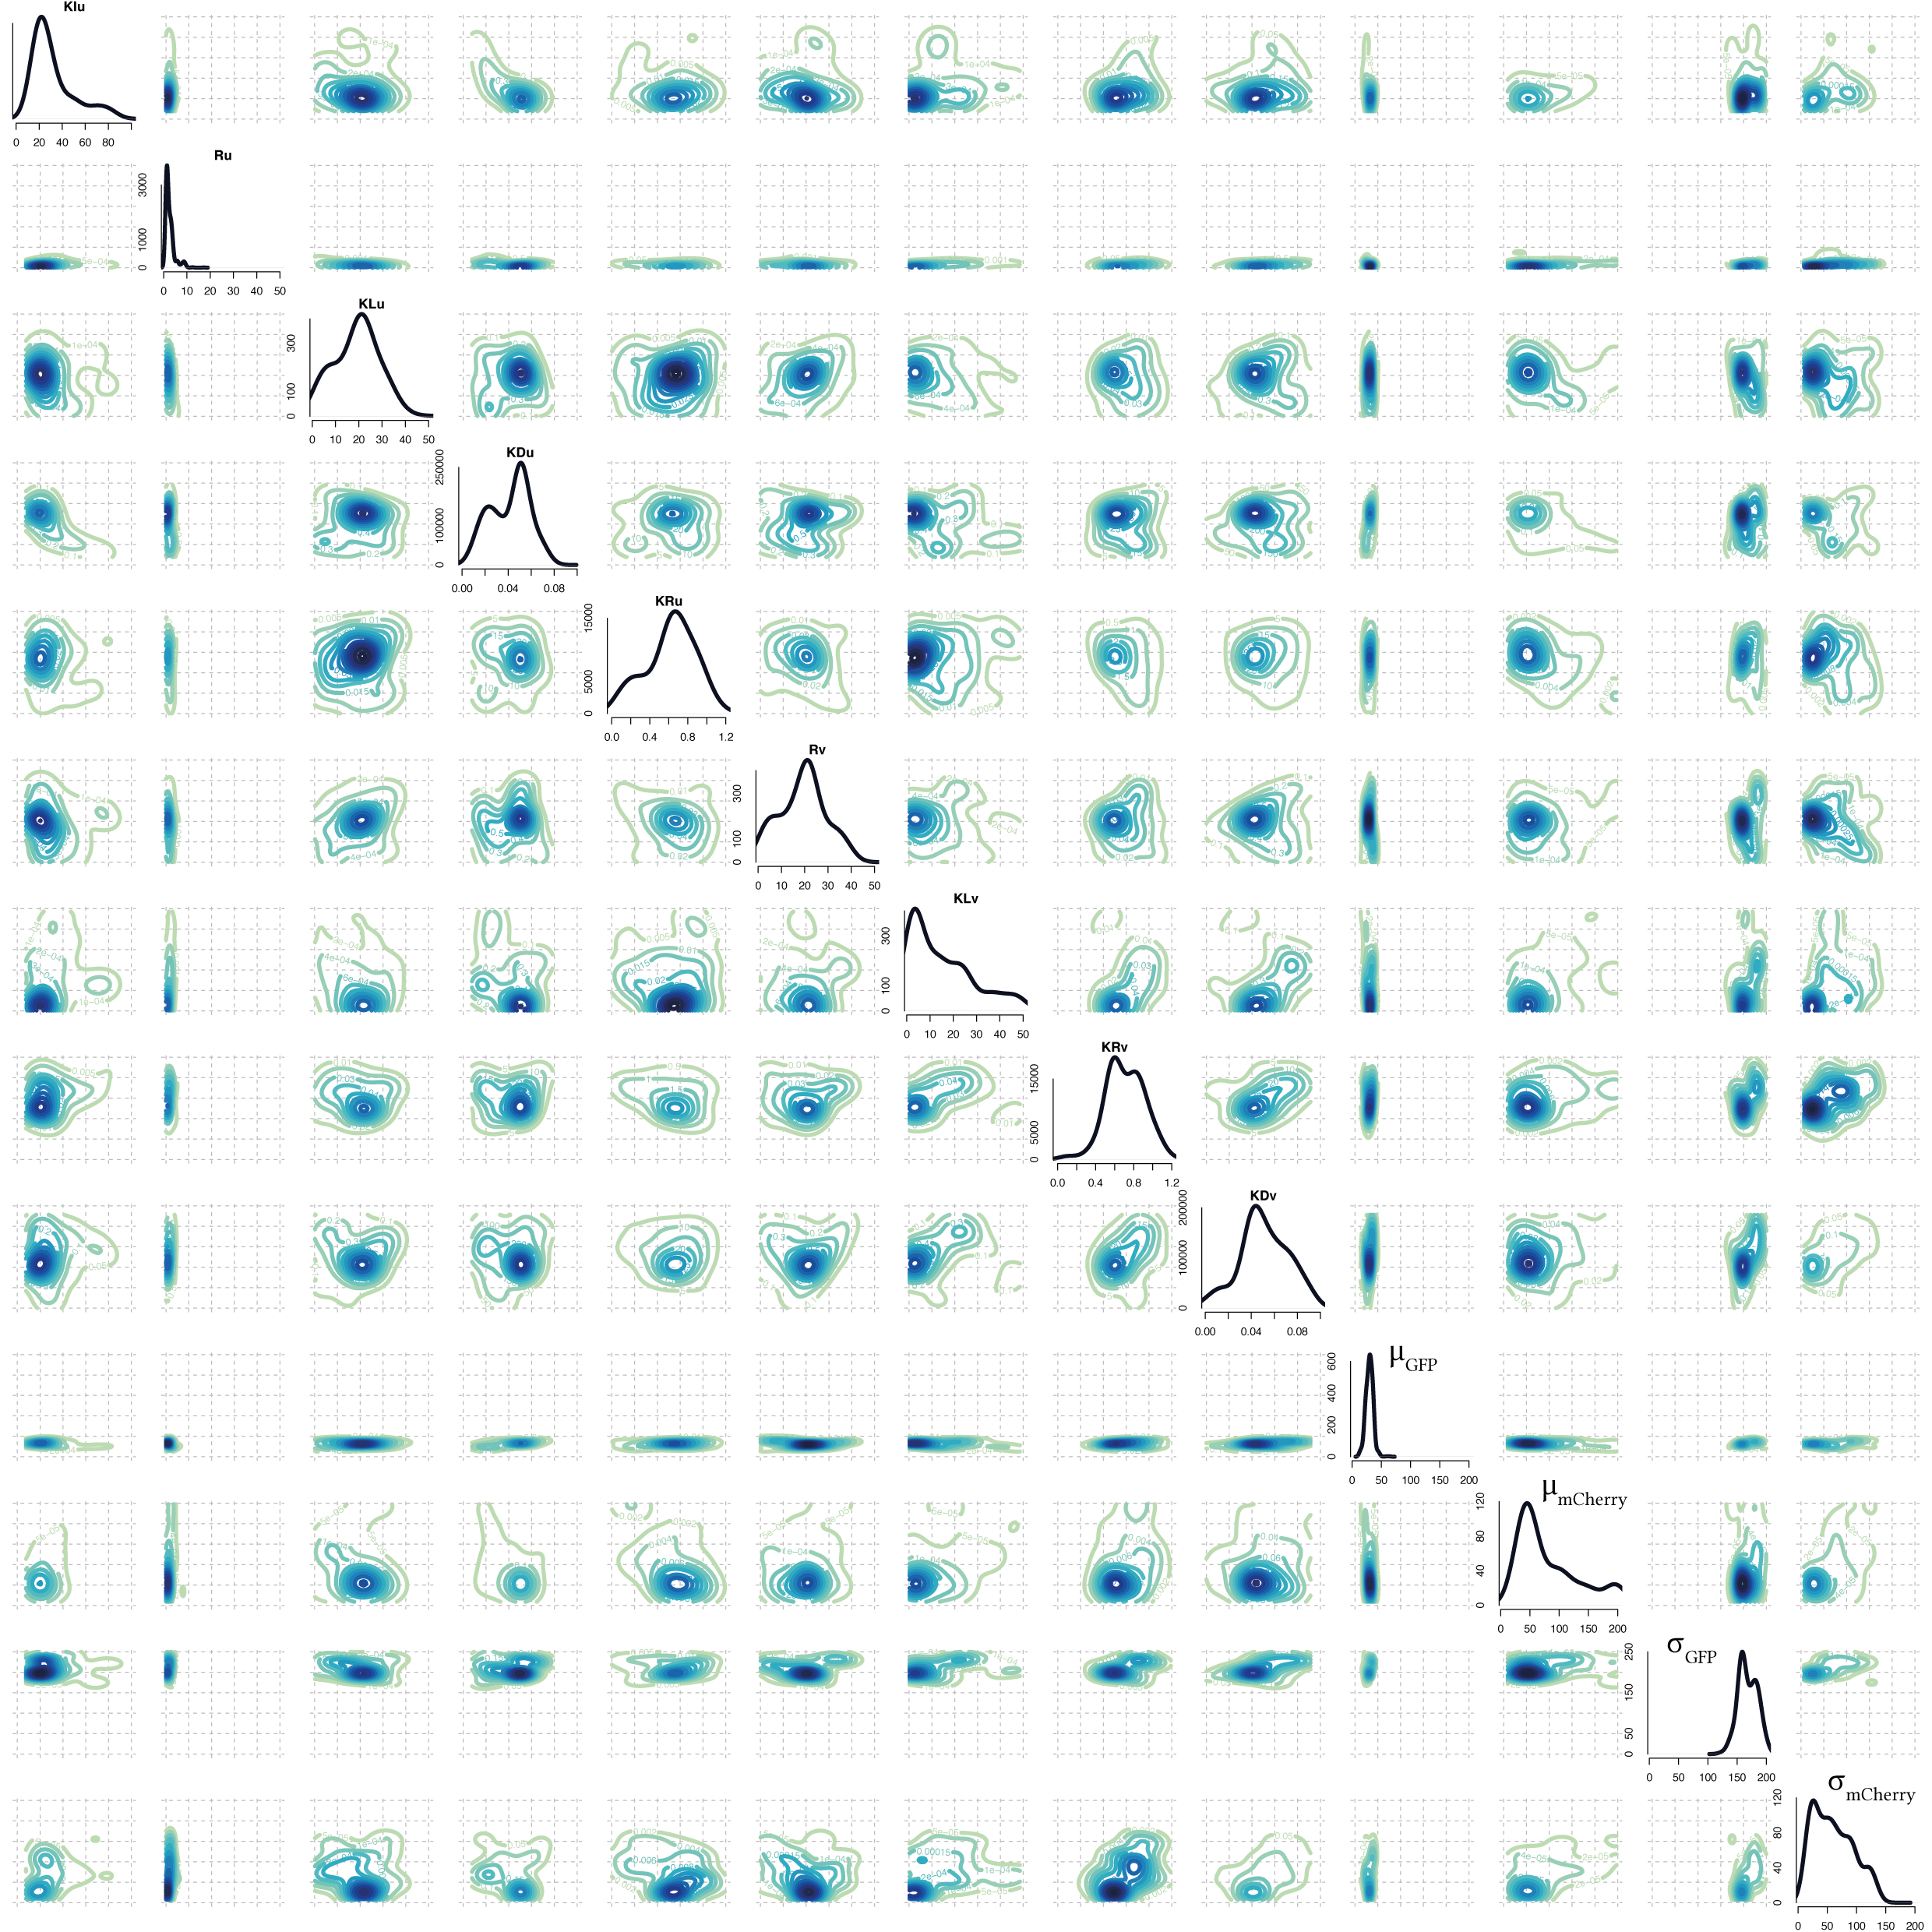
\includegraphics[width=1.1\textwidth]{../../chapters/chapterABCFlow/images/posterior_iptg.png}
	\caption[Posterior distribution of inferred parameters for post-IPTG induction of the toggle switch]{\label{fig:1atc-post} The posterior distribution obtained from ABC-Flow for the post-IPTG time course data. The parameter for GFP expression (R\textsubscript{u}) was found to be the most well inferred.}
\end{figure}

The two fits obtained from the post-\acrshort{atc} and post-IPTG induction represent the different sides of the switch from the same genetic system and should thus be considered together. Comparing the fits we find a good agreement for the inferred parameters R\textsubscript{u} and KD\textsubscript{u}. On the other hand we find that the inferred values for KR\textsubscript{u} and KD\textsubscript{v} do not agree. This could be caused by the fact that the switch is not perfectly symmetric on the two sides, as can be seen from the experimental data. The system responds to \acrshort{atc} faster than to IPTG. This difference in the data could lead to difference values inferred for the underlying parameters. In the future this could be incorporated in to ABC-Flow to improve the accuracy of the inference.



%\begin{figure}[tb]
%\centerfloat
%	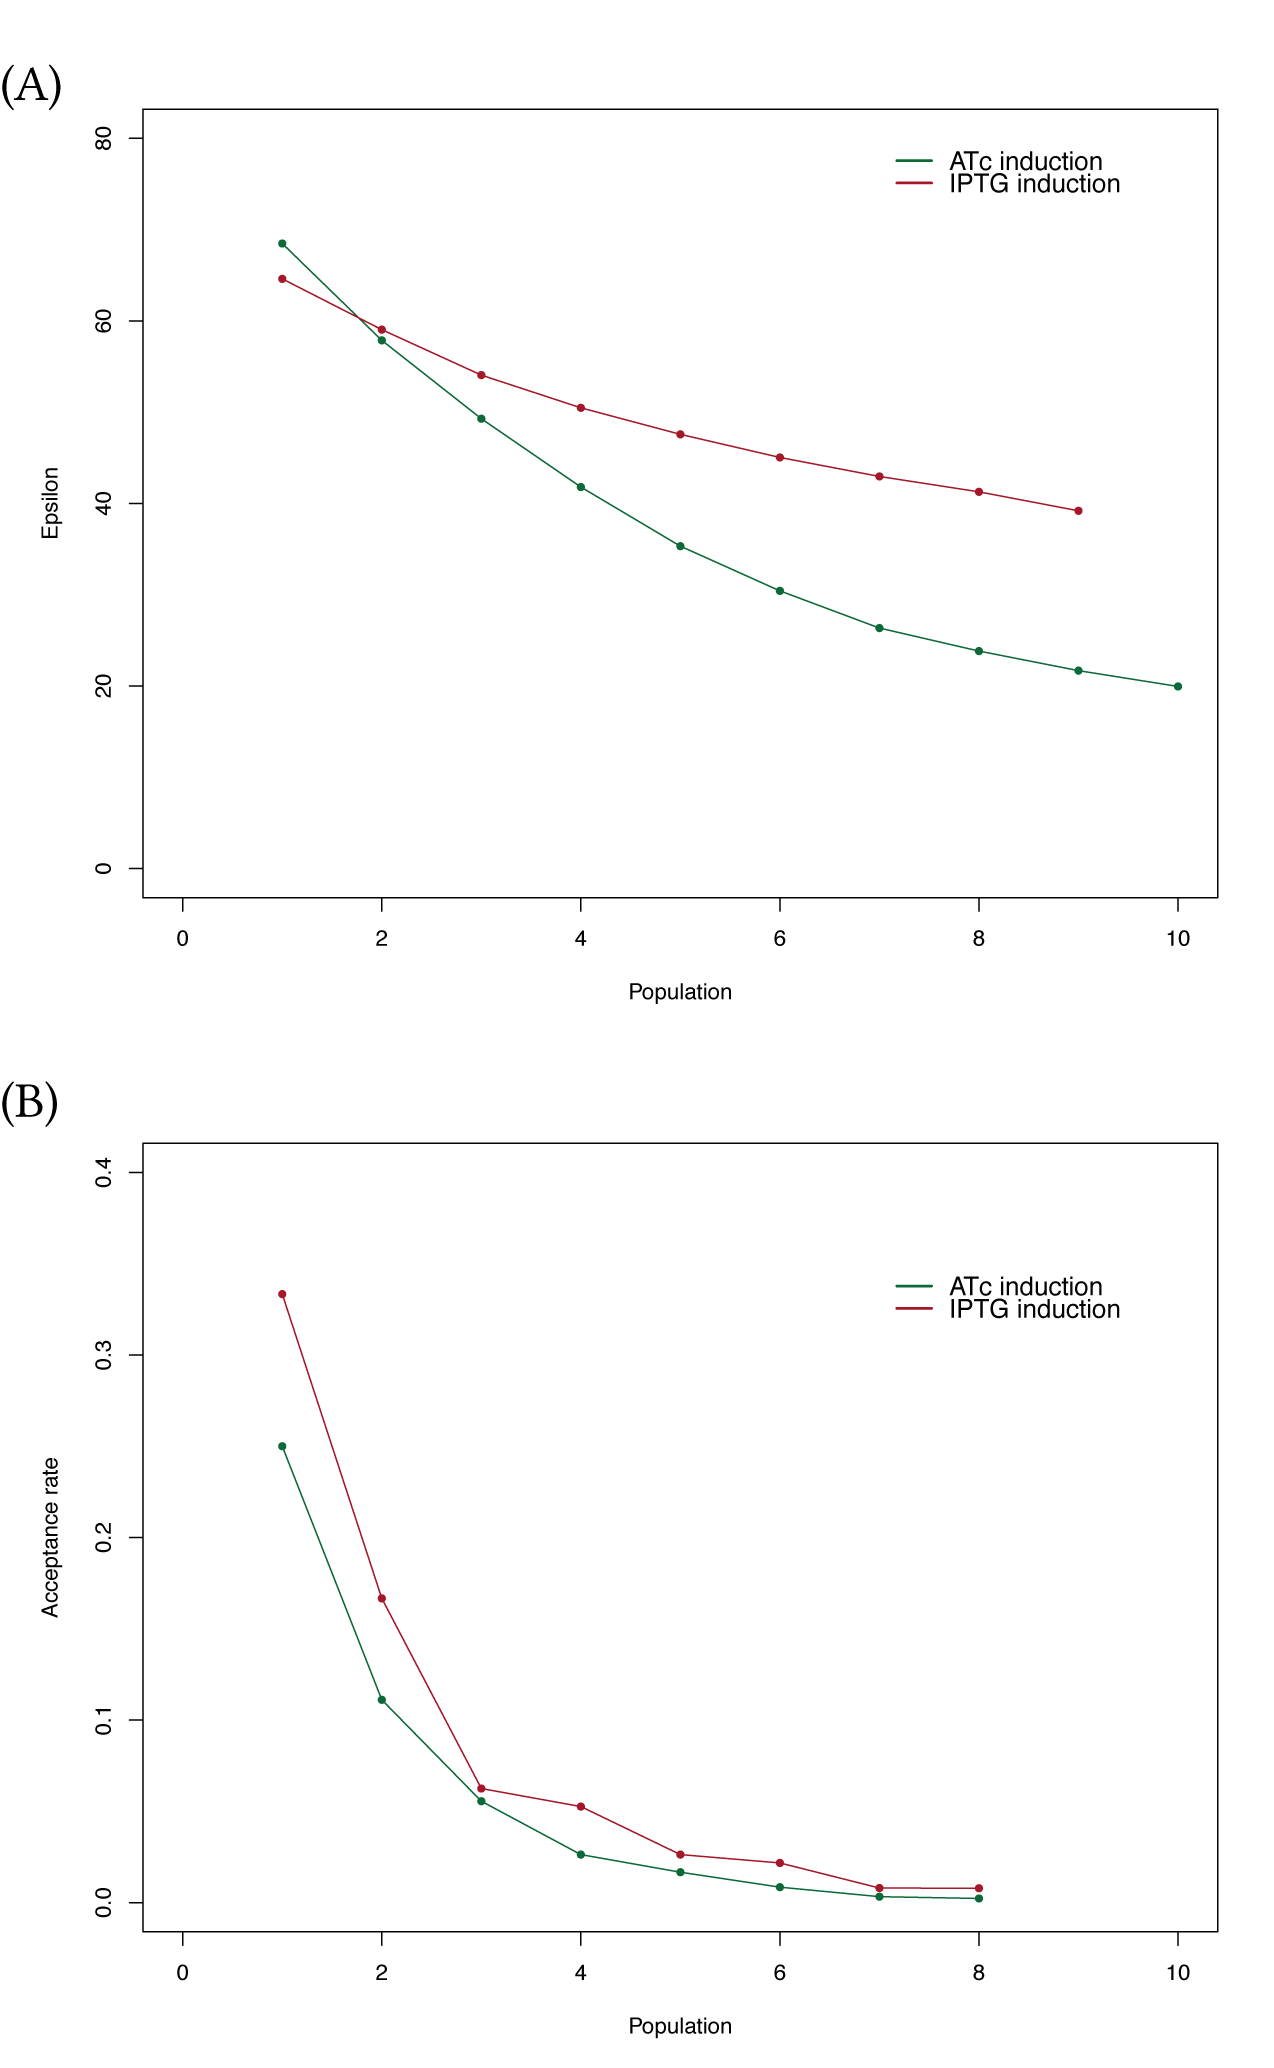
\includegraphics[scale=0.7]{../../chapters/chapterABCFlow/images/epsilon_acceptance.png}
%	\caption[Epsilon and acceptance rate of ABC-Flow inference]{\label{fig:epsilon_accept}(A) The progression of epsilons over the populations in ABC-Flow for ATc (green) and IPTG (red) induction. (B) The acceptance rate decreases rapidly with every population.}
%\end{figure}

In this section I used ABC-Flow to fit a toggle switch model to experimental flow cytometry data. Both sides of the switch were examined, \acrshort{atc} induction which flips the switch from mCherry high to GFP high and IPTG induction, which flips the switch from GFP high/mCherry low to GFP low/mCherry high. The model was successfully fit to the data set obtained from the ATc induction of the switch but less so to the data obtained from the IPTG induction of the switch. 
%\clearpage
\section{Discussion}

In this Chapter I characterised the genetic toggle switch experimentally. First I studied the effect of the two inducers \acrshort{atc} and \acrshort{iptg} on the growth rate of the selected chassis \textit{E. coli} K-12 MG1655. I find that there is no detrimental effect to the bacterium by the inducers. I further characterised the switch by determining the minimum inducer concentration necessary to change the state of the switch. I find that for \acrshort{atc} induction, a minimum of \SI{0.09}{\nano\gram\per\milli\liter} is required to cause the switch to go to a GFP high state. For \acrshort{iptg} induction I find that a minimum of \SI{0.001}{M} is required to flip the switch to an mCherry high state. This information is critical for using this switch in other applications. Both sides of the switch are very sensitive to inducer concentrations, as the concentrations required to observe a change in fluorescence are very small. Further, I found that the switch is instantaneous for both GFP and mCherry, with no intermediate fluorescence levels observed. 

Furthermore I found that this toggle switch, pKDL071, is faster to respond to a change in \acrshort{atc} concentration that to a change in \acrshort{iptg} concentration. For \acrshort{iptg} induction we observe a change in fluorescence after 3-4 hours of induction. For \acrshort{atc} induction we can see a difference within an hour of induction. This result is in agreement with~\textcite{Litcofsky:2012gr}. This difference in response times must be taken into account when using the pKDL071 switch for other applications. This difference could be attributed to maturation times of the fluorescent proteins. \textcite{Macdonald:2012el} found that mCherry half-maturation time is 150 mins, whereas the GFP variant used here, GFPmut3b has been especially mutated for fast action~\autocite{Cormack:1996gv}.~\textcite{Cormack:1996gv} found that whereas wild type GFP is detectable 1-2 hours after induction, GFPmut3b is detectable 8 minutes after induction. This difference could account for the different response times observed.

Here I also developed a Bayesian framework, ABC-Flow, that is used to fit stochastic models to flow cytometry data. Fitting computational models to flow cytometry data can be challenging; fluorescence intensity is measured in arbitrary units and there can be a big variability between experiments depending on instrument settings. This poses a challenge for model fitting as the fluorescence intensity emitted by each individual fluorophore molecule cannot be reliably estimated~\autocite{Kelwick:2014iy}. ABC-Flow converts the number of molecules obtained via simulations to fluorescence intensity in order to overcome current limitations in fitting computational models to flow cytometry data. The novelty of ABC-Flow is that it can be used on two-dimensional flow cytometry data. Unlike ~\textcite{Lillacci:2013hu}, it can be used to infer the parameter values of systems involving one or two fluorescent molecules. This makes it ideal to be used on the genetic toggle switch, whose behaviour is reflected by the levels of two fluorescent proteins, GFP and mCherry.

I have used ABC-Flow to fit the toggle switch model to simulated flow cytometry data in one and two dimensions. This demonstrated the effectiveness of ABC-Flow in parameter identifiability of intensity data. Further, I used ABC-Flow to fit a stochastic computational model to flow cytometry time course data obtained by inducing the genetic toggle switch to its two states. This was done using both sides of the switch, GFP high/mCherry low to GFP low/mCherry high using IPTG and vice versa using \acrshort{atc}. The model parameters were inferred from the data obtained via \acrshort{atc} induction, representing the flip from GFP low/mCherry high to GFP high/mCherry low. The inferred parameter values were used to make predictions on the behaviour of the toggle switch system under different initial conditions, promoter and repression strengths. The parameters were not inferred as well for the data obtained via IPTG induction. This could be attributed to the experimental data obtained. Post-IPTG induction we observed a decrease in GFP but the increase in mCherry was not as prominent. This result could be improved by a repetition of the time course experiment, which was not carried out due to time constraints.


The model fits to experimental data presented here could be improved by a number of ways in the future. Firstly, the toggle switch model used here was a simplified version of the system. The model consisted of two proteins, GFP and mCherry and used the Shea-Ackers formalism. A more flexible and detailed model, like one built using mass action kinetics and including LacI and TetR could lead to more accurate inference. It would also allow to test more aspects of the system via simulations using the inferred parameters. It must  be noted that the intensity model used here assumes a normal distribution without any correlation. It does not include the correlation between GFP and mCherry and the two intensity normals are inferred independently. This is not the case in the experimental data collected, where a correlation between the two is observed. In addition, the model fits would be improved if the flow cytometry data was further pre-processed by calibration using commercially available calibration beads. Computational methods like FlowCal, developed by~\textcite{Tabor:2009bz} can be used to convert fluorescence arbitrary units (a.u.) to MEFs (molecules of equivalent fluorophore). This can account for instrument gain settings as well as day to day instrument variability. Future improvements on ABC-Flow could also include the simultaneous fitting of the toggle switch model to both time courses, post-\acrshort{atc} and post-IPTG induction. Both of these time courses are obtained from the same genetic system, and the accurate characterisation of said system would have to include both functions. This would allow us to obtain parameter estimates for components that can respond to both inducers. ABC-Flow could be also be further developed to be able to fit computational models to more fluorophores simultaneously. This would enable the effective characterisation of more complex systems.



 %I also find that which state the switch is on has no effect on the growth rate of the bacteria. In order for this toggle switch to be used in a synthetic biology application, it is important that both sides of the switch have an equivalent burden onto the chassis. If one of the steady states creates a larger burden and slows down the growth of the bacteria, this can create an imbalance in the population. If the toggle switch-bearing bacterial population exists in an environment with competing bacteria, for example the gut microbiome, and one of the two states creates a larger burden, this would cause the switch-bearing population to become less competitive compared to the non switch-bearing population. It is therefore crucial that the state of the switch does not affect the competitiveness of the chassis.  

%%%%%%%%%%%%%%%%%%%%%%%%%%%%%%%%%%
%%%This bit include it but has to be linked between experiments and modeling 
%This difference is also observed in the fitted computational models of the system. The computational model used here to fit these time course data did not account for fluorophore maturation time, as a summary parameter of GFP production was used instead. A more detailed model could be used to further investigate this difference. Since ABC-Flow simulates the models in order to obtain the posterior density, the size of the model will not be an obstacle in parameter estimation.
%%%%%%%%%%%%%%%%%%%%%%%%%%%%%%%%%%

%The use of computational models is crucial to understand the complex processes underlying observed biological phenomena~\autocite{Lillacci:2013hu}. This has proved especially important in the advancement of synthetic biology, which strives to produce systems with well-defined functions~\autocite{Chin:2006fb} and reliable operation~\autocite{Lu:2009ez}. Being able to have a well-parameterised model of a synthetic gene network can aid in the reliable use of such system. It can also aid in the further design and improvement of the synthetic system. Further modifications to the synthetic gene network can be tested \textit{in silico}. 


The framework developed here can aid the advance of the understanding of genetic systems. ABC-Flow can be used to characterize a system under study, and infer the parameter values that give rise to the experimental flow cytometry data. This will allow the accurate parameterisation of computational models describing the system, a known bottleneck in quantitative model building~\autocite{LeNovere:2015dp}. A parameterised model can be used to further the understanding of the system and make testable predictions for its behaviour. It can be used to study how the fluxes and concentrations of the species are influenced by the parameter values~\autocite{Li:2010kt}, such as transcription or translation rate. This allows for the prediction of the response of the system under different stresses \textit{in silico}. The different parts of the system under study, working together to produce the response observed, can be disentangled, understood and studied separately without the need for numerous laborious and time consuming experiments. 


\section{Summary}


In this chapter I developed ABC-Flow, a Bayesian framework used to fit computational models to flow cytometry data. I tested the method using simulated data. I summarised the experiments carried out for the analysis of the genetic toggle switch. I used the pKDL071 plasmid and characterised its switching behaviour over various inducer concentrations and over time. I found the concentration of each inducer necessary to flip the switch as well as the time it takes for the change to be observed. The time course experiments were used as input to ABC-Flow in order to fit a computational model to the data and infer the parameter values. In the next Chapter I outline an experimental design to construct more robust genetic toggle switches.


 %Furthermore, I investigated the effect of the inducers on the growth rate of the chassis and found that they have no effect. In the next chapter I use the data collected in the chapter to fit to the more realistic toggle switch models used in Chapter (XXX). 





 
 